% TEMPLATE for Usenix papers, specifically to meet requirements of
%  USENIX '05
% originally a template for producing IEEE-format articles using LaTeX.
%   written by Matthew Ward, CS Department, Worcester Polytechnic Institute.
% adapted by David Beazley for his excellent SWIG paper in Proceedings,
%   Tcl 96
% turned into a smartass generic template by De Clarke, with thanks to
%   both the above pioneers
% use at your own risk.  Complaints to /dev/null.
% make it two column with no page numbering, default is 10 point

% Munged by Fred Douglis <douglis@research.att.com> 10/97 to separate
% the .sty file from the LaTeX source template, so that people can
% more easily include the .sty file into an existing document.  Also
% changed to more closely follow the style guidelines as represented
% by the Word sample file. 

% Note that since 2010, USENIX does not require endnotes. If you want
% foot of page notes, don't include the endnotes package in the 
% usepackage command, below.

% This version uses the latex2e styles, not the very ancient 2.09 stuff.

\documentclass[10pt]{usetex-v1-tight}
\usepackage{xcolor}
\usepackage{enumerate}
\usepackage{enumitem}
\usepackage{amssymb}
\usepackage{graphicx}
\usepackage{subfigure}
\usepackage{url}
\usepackage{xspace}
\usepackage{todonotes}
\usepackage[hyperfootnotes=false,breaklinks]{hyperref}
\hypersetup{
	colorlinks,
	citecolor=red,
	linkcolor=blue,
	urlcolor=blue
}

\usepackage[linesnumbered,ruled,vlined]{algorithm2e} 
\SetVlineSkip{0pt} 
%\usepackage{algorithmic}

\usepackage{cleveref}
\crefname{section}{\S}{\S\S}
\Crefname{section}{\S}{\S\S}

\newlength{\gapspace}
\newcommand{\gap}[1][0cm]{\setlength{\gapspace}{#1}\vspace{.5\gapspace}\textbf{\color{red}[...]}\vspace{.5\gapspace}\xspace}

\newcommand{\NZ}[1]{\noindent\textcolor{blue}{\bf $\blacksquare$ Nannan: #1}}
\newcommand{\VT}[1]{\noindent\textcolor{orange}{\bf $\blacksquare$ Vasily: #1}}
\newcommand{\HA}[1]{\noindent\textcolor{red}{\bf $\blacksquare$ Hadeel: #1}}
\newcommand{\LR}[1]{\noindent\textcolor{cyan}{\bf $\blacksquare$ Lukas: #1}}
\newcommand{\DIM}[1]{\noindent\textcolor{olive}{\bf $\blacksquare$ Dimitris: #1}}
\newcommand{\Ali}[1]{\noindent\textcolor{green}{\bf $\blacksquare$ Ali: #1}}

\newcommand{\abc}[1]{\noindent\textcolor{red}{\bf $\blacksquare$ AB: #1}}

\newcommand{\arb}[1]{\todo[inline,color=red]{\textcolor{white}{ARB: #1}}}

\newcommand{\ie}{i.e.\ }
\newcommand{\eg}{e.g.,\ }
\newcommand{\etal}{et al.~}
\newcommand{\vs}{vs.\ }
\newcommand{\cf}{cf.~}

\newcommand{\sysname}{Sift\xspace}

 % lukas: a more compact itemize/enumerate environment to save space and better looks
\newenvironment{compactitemize}{%
\begin{itemize}[leftmargin=1em, itemsep=0em, parsep=0em, topsep=.1em, partopsep=.1em]}
{\end{itemize}}
\newenvironment{compactenumerate}{%
\begin{enumerate}[leftmargin=1em, itemsep=0em, parsep=0em, topsep=.1em,partopsep=.1em]}
{\end{enumerate}}

\begin{document}

%don't want date printed
%\date{}

%make title bold and 14 pt font (Latex default is non-bold, 16 pt)
\title{
	%Registry Diet: Weight Loss Secrets for Docker Registry\\
%Weight Loss Secrets for Docker Registry\\
\sysname: Fast and Lightweight Docker Registries
%\\
%Applying Deduplication to Docker Registry\\
%Why and How to Apply Deduplication to Docker Registry
}


\author{
	{\rm Nannan Zhao$^{1}$,
		%Vasily Tarasov$^{2}$,
		Hadeel Albahar$^{1}$,
		Subil Abraham$^{1}$,
		Ali Anwar$^{2}$},
	%{\rm Lukas Rupprecht$^{2}$, 
	%	 Dimitrios Skourtis$^{2}$,}\\
	%{\rm Amit S. Warke$^{2}$,
	%	Mohamed Mohamed$^{2}$, 
	%	Dean Hildebrand$^{2}$\thanks{Now at Google.}
	and Ali R. Butt$^{1}$\\
	{{$^1$}{Virginia Tech}, {$^{2}$}{IBM Research---Almaden}}
}

\maketitle

% Use the following at camera-ready time to suppress page numbers.
% Comment it out when you first submit the paper for review.
\thispagestyle{empty}

\begin{abstract}

\vspace{-6pt}
%
The rapidly growing number of container images and the associated storage
performance and capacity requirements are the key obstacles to efficiently
scaling Docker registries.
%
Though the real-world images contain a tremendous amount of duplicate data,
modern registries cannot effectively eliminate the duplicates due to the
compressed format of the images.
%
In this paper, we propose a new Docker registry architecture, \emph{\sysname},
that integrates deduplication into the Docker registry.
%
\sysname supports several configurable deduplication modes that provide
different levels of storage efficiency, durability, and performance, as desired
by different use cases.
%
Further, to mitigate the negative impact of deduplication on the image download
and upload times, \sysname introduces a two-tier cache with a novel
user-access-history-based prefetch algorithm. 
%
Under real workloads, \sysname saves up to XXX\% of storage space while keeping
the latencies within the XXX\% of the original registry.

%The approach enables it to achieve a $96$\% hit ratio and save $56$\% more
%cache space.

%Based on our 

%sustaining and scaling container systems in the face of exponential growth is challenging. 
%%
%For example, Docker Hub~\cite{docker-hub}---a popular public container registry---stores more than~2 million public repositories. These repositories have grown at the rate of about $1$ million annually---requiring provisioning an additional 2.5~TB of storage per week on average---and the rate is expected to increase.
%%
%This puts intense pressure on Docker registry storage infrastructure, but the problem has so far remained largely unexplored.
%

\end{abstract}

%we predict  
%Overall,  
%to model the deduplication for estimating the deduplication effect on performance and storage savings, especially in terms of deduplication rate and deduplication overhead. We propose to use Markov decision process to find optimal solution that can maximize the storage saving and minimizing the cost in terms of performance degradation. Our solution will largely reduce the amount of redundant data in container storage systems and outperform the state-of-art deduplication techniques without any performance overhead.

%and evaluate
%the potential of file-level deduplication in the registry.
%
%Our analysis reveals that 
%
%We then present the design of \sysname---a Docker registry with file deduplication
%support---and conduct a simulation-based analysis of its performance implications.

\section{Introduction}
 
Containers have become a prominent solution for deploying modern applications because to their tight isolation, low overhead, and efficient packaging of the execution environment~\cite{docker}.
Containers are the running instances of \emph{images} which contain the complete runtime environment for an application.
An image comprises a set of shareable and content addressable \emph{layers}.
% and is stored in Docker \emph{registry}. 
Each layer is a set of files that are compressed in a single archive. 
Docker images/layers are stored in an online store called Docker registry~\cite{docker-hub} and accessed by clients as needed.
%As layers are the building blocks of images, they can be shared among multiple images. 
Since layers are uniquely identified by a collision-resistant hash of its content, 
no duplicate layers are stored in the registry.
Many container registries use remote cloud storage like S3~\cite{s3}, 
Microsoft Azure~\cite{azure}, and OpenStack Swift~\cite{swift} as their backend storage systems~(Figure~\ref{fig:without-dedup}).
%For example, Google container Registry~\cite{GoogleContainerRegistry} stores images on Google cloud storage while
%IBM container registry uses IBM cloud to manage image storage.

The amount of images stored in Docker registries is increasing dramatically.
%Docker registries store a large amount of images and with the increasing popularity of Docker, registries continue to grow. 
For example, Docker Hub~\cite{docker-hub}---a popular public registry---stores more than~2 million public repositories that host one or more images. 
We observed that the number of public repositories grows by around~1 million annually. 
We estimate that~1 million annual growth in the number of repositories 
amounts to about~130\,TB storage space required per year.
%Moreover, 
%just storing~130\,TB worth of Docker images on Google cloud will cost around~\$14,000 per month~\cite{GoogleCloudStoragePricing}.
This massive amount of image dataset presents great challenges for Docker registry storage infrastructure and so far has remained largely unexplored.
%Then, the 1 million annual growth in the number of repositories amounts to about 130\,TB, costing around~\$15,000 a month.

\paragraph{Deduplication}
Our analysis of around~47\,TB (167\,TB uncompressed) of Docker images downloaded from Docker Hub,
which in total contain over~5 billion files, reveals that
that only~3\% of the files are unique while others are redundant copies. 
%Since many Docker images share many underlying layers, 
This suggests that current layer sharing mechanism cannot efficiently remove data duplicates.
%current
% considerable file-level redundancy across different images is not mitigated by Docker's existing layer sharing mechanism.
Many cloud storage systems already implemented deduplication to effectively eliminate redundant data.
%\NZ{let use redundant data instead of redundancy}
For example,
Google cloud and AWS, 
perform in-line data deduplication transparently.\NZ{use a new example}
However, existing deduplication techniques cannot be directly applied to the image storage system 
because of unique dataset in the Docker registry: compressed layers. 
In contrast to uncompressed files, compressed files have a lower deduplication ratio. 
So layers should be decompressed before performing deduplication.

As shown in Figure~\ref{fig:with-dedup}, 
after decompression and simple file-level deduplication, the unique files may get scattered on
multiple servers. 
To restore a layer,
the layer's containing files should be first fetched from multiple servers, then compressed as a layer
and sent back to the client.
The extra network, I/O, and computation latency will slow down the response time for pulling an image.

%Without deduplication (Figure~\ref{fig:without-dedup}),
%the average latency for requesting a layer is around~2\,s for layers with size less than~50\,MB.
%The latency increases to~12\,s when deduplication is implemented in the backend storage system.
%Furthermore, Docker registry performance drops down dramatically for bigger layers.

%We observe that the average latency for requesting layers larger than~50\,MB and smaller than~1\,GB
%is around~128\,s. The latency worsens when dedupliation is implemented, with an average around~800\,s.
%incurs a considerable additional overhead on layer pull time and thus affecting the overall container startup time. 
%A solution would be to decompress the layers before applying deduplication on Docker registries.
 
%Therefore, in this paper, we propose a new Docker registry architecture,~\sysname,
%that integrates caching and deduplication with Docker registries to address the aforementioned obstacles.
%low restore latency %adaptive%
% deduplication framework for Docker registries. 

\paragraph{Caching}
Large container registry service providers like Google and IBM use regional private registries across the world to facilitate a fast and high-availability service~\cite{GoogleContainerRegistry,ibmregistry}.  
This geographical distribution allows users to store images near their compute instances and experience a fast response time. 
Deploying these registries as a cache, temporarily storing popular layers,
to improve pull latency may be intuitive.
%Although cache has been studied as web cache or proxy cache, 
However, there are unique challenges in integrating a cache with deduplication in Docker registry.
%%%%
%we can use registry as a web/proxy cache because registry already has been deployed regionally close to clients to speedup performance. although there are so many works on web/proxy cache but you cannot just use it with docker registry because of the following challenges. 
%%%%
First, we observe that layer sizes vary from a few MB to several GB and that majority of layers are around several MB.
A small main memory cache cannot accommodate many popular layers.
Second, 
Although layer pull requests are heavily skewed, we observed that the duration between two subsequent requests is too long. 
Meaning, if we cache a layer, we might need to wait hours to get a hit on that layer.

\paragraph{~\sysname}
In this paper, we propose a new Docker registry architecture,~\sysname,
that integrates caching and deduplication with Docker registries to address the aforementioned obstacles.
%To address these issues,
~\sysname~embodies a two-tier heterogeneous cache architecture 
comprising a layer buffer and a file cache to hold even more popular layers:
The layer buffer stores popular layers in main memory while the file cache stores 
the \emph{deduped} unique files for the victim layers that are evicted from the layer buffer on a 
flash-based storage system to improve cache space utilization.
Moreover, we proposed a user-based cache algorithm to improve the cache hit ratio 
because we observed that user active time is more predictable.

%Moreover, to improve layer pull performance, we design a user behavior based cache. 
%The cache adaptively stores a certain amount of active users' layers, in a layer buffer, to speed up active users' pull time. 
%The cache also selectively stores a few popular \textit{shared} and \textit{deduplicated} files, in a file cache, to accelerate the layer restoring process. 
%The rationale behind the user behavior based cache is that, instead of only focusing on layer-level access pattern, 
%we consider the user behavior for cache replacement because users' behavior is more predictable than layer access pattern. 
%Moreover, users are the ones who issue the layer/manifest pulls and pushes.  
%For this reason, our cache replacement policy is an adaptive heuristic, top-down decision making process driven by users' behavior.
%During cache eviction, we evict the least recently accessed layer from a set of candidate layers exclusively referenced by the least recently active users to make room for new users' layers. 
%After an inactive user's layer is evicted from the layer buffer, based on our algorithm, it can either be discarded or hosted in the file cache. For the latter, the layer will undergo offline decompression and file-level deduplication.
%For the incoming new users, we prefetch a number of their repositories along with their containing layers based on their access probabilities.

We evaluate our proposed design, \sysname. 
\sysname~acheives a hit ratio~20\% higher than that of traditional LRU. 
%by conducting a preliminary simulation-based study. Our study aims to explore the feasibility/benefits of deduplication and quantify the overhead it introduces.
\HA{plz add preliminary results}.  

\begin{figure}[t]
	\centering
		\begin{minipage}{0.225\textwidth}
			\centering
			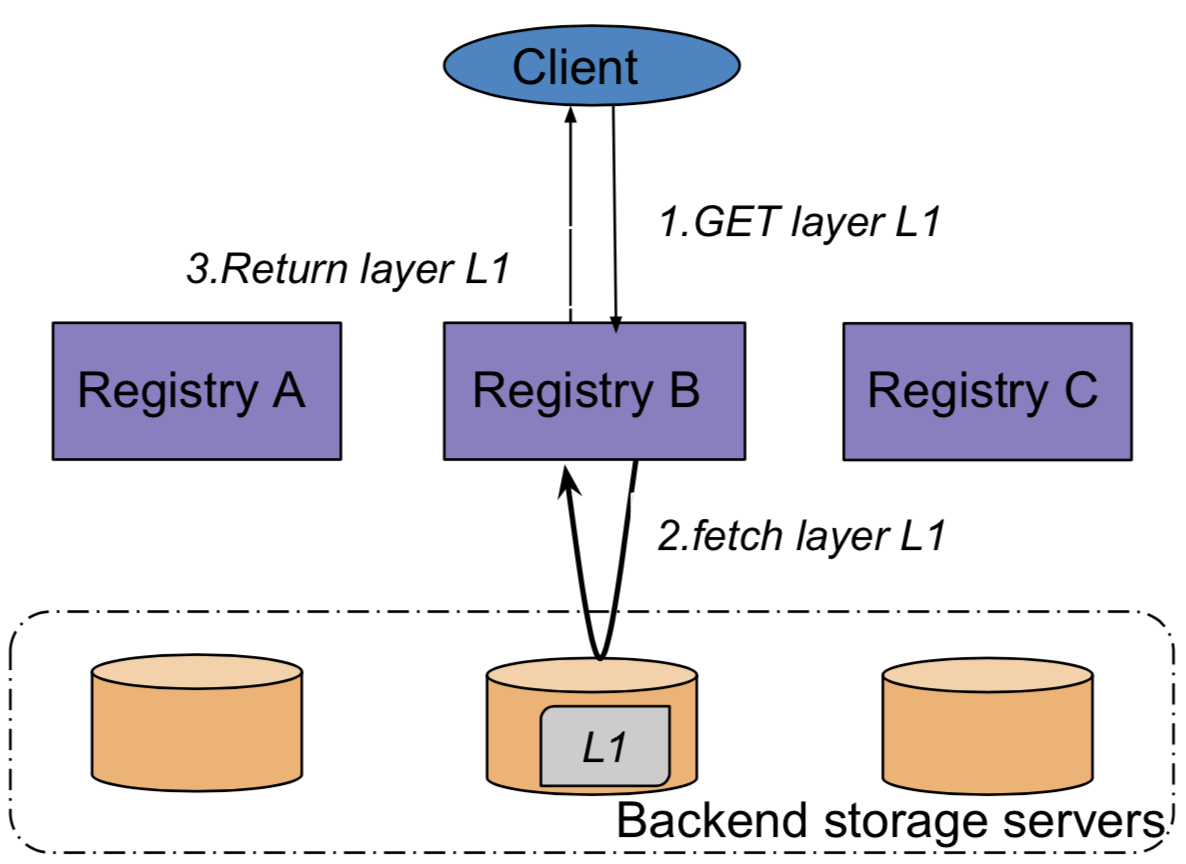
\includegraphics[width=1\textwidth]{graphs/nodedup.png}
			\caption{CDF of layer reference count.}
			\label{fig:ref_count}
		\end{minipage}
	\begin{minipage}{0.225\textwidth}
		\centering
		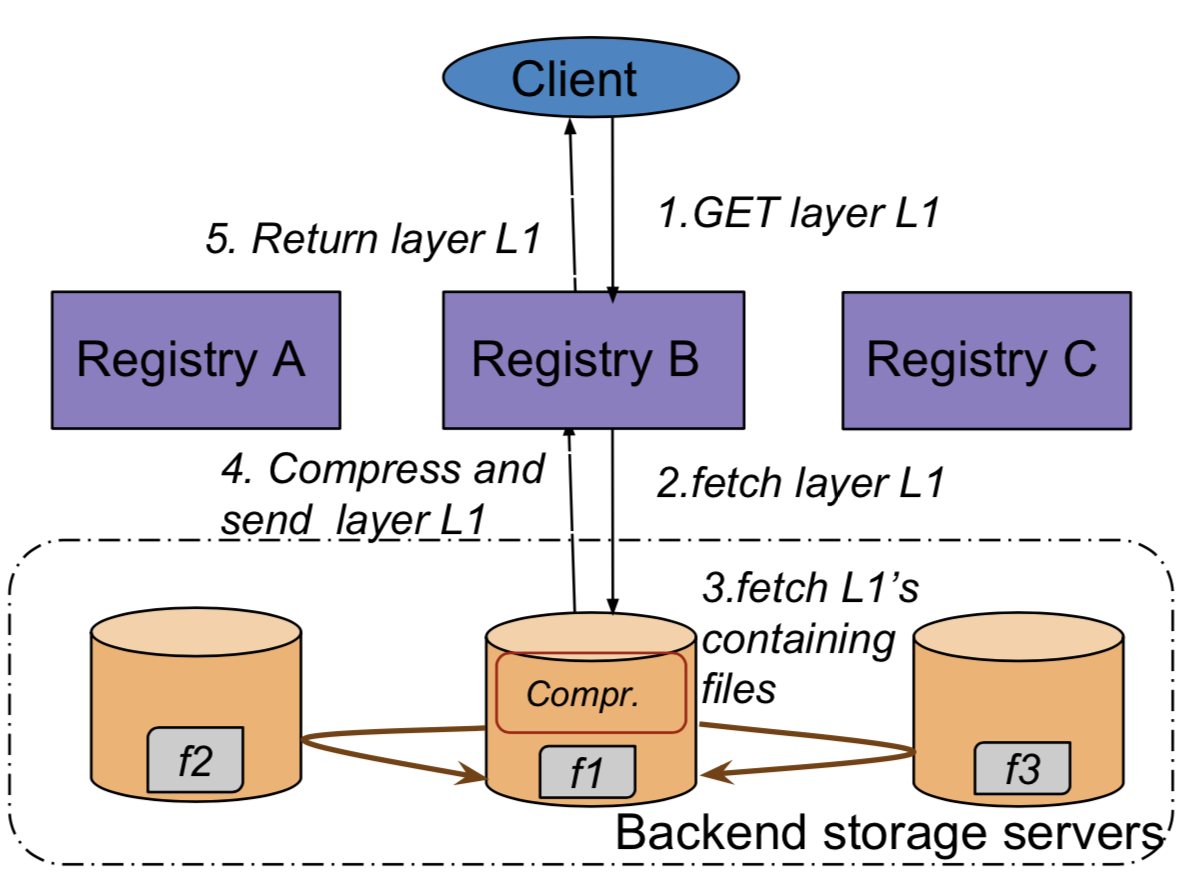
\includegraphics[width=1\textwidth]{graphs/dedup.png}
		\caption{CDF of compress. and uncompress. layer size.}
		\vspace{-3pt}
		\label{fig:nodedup-vs-dedup}
	\end{minipage}
\end{figure}

%\HA{need to mention Figure~\ref{fig:without-dedup} and Figure~\ref{fig:with-dedup}}

The organization of this paper as follows: 
We explain relevant Docker details along with observations and current deduplication practices in production registries in~\cref{sec:background}.
We present~\sysname~in~\cref{sec:\sysname} and ~\sysname's preliminary evaluation in~\cref{sec:Evaluation}. 
We discuss related work in~\cref{sec:related}.
Lastly, we conclude and discuss in~\cref{sec:conclusion} and~\cref{sec:discussion}.

%%%%%%%%%%%%%%%%%%%%%%%%%%%%%%%%%%%%%%%%%%%%%%%%%%%%%%%%%%%%%%%%%%%%%%%%%%%%%%
%                                                                            %
%                                OLD INTRO                                   %
%                                                                            %
%%%%%%%%%%%%%%%%%%%%%%%%%%%%%%%%%%%%%%%%%%%%%%%%%%%%%%%%%%%%%%%%%%%%%%%%%%%%%%

%\emph{Containers}~\cite{process-containers-linux} have recently gained
%significant traction due to their low overhead, fast deployment, and
%the rise of container management frameworks such as Docker~\cite{docker}.
%%
%Polls suggest that 87\% of enterprises are at various stages of adopting
%containers, and they are expected to constitute a \$2.7 billion
%market by 2020~\cite{container-grow-by2020}.
%
%Docker combines process containerization with efficient and effective packaging
%of complete runtime environments in so called {\em images}.
%%
%Images are composed of shareable and content addressable {\em layers}.
%%
%A layer is a set of files, which are compressed in a single archive.
%%
%Both images and layers are stored in a Docker \emph{registry} and accessed by
%clients as needed.
%%
%Since layers are uniquely identified by a collision-resistant hash of
%their content, no duplicate layers are stored in the registry.
%
%Registries are growing rapidly.
%%
%For example, Docker Hub~\cite{docker-hub}, the most widely used registry,
%stores more than 500,000 public image repositories comprising over 2 million
%layers and it keeps growing.
%%
%Over a period from June to September 2017, we observed a linear growth of the number
%of images in Docker Hub with an average creation rate of 1,241 repositories per day.
%%
%We expect this trend to continue as containers gain more popularity.
%%
%This massive image dataset presents challenges to the registry storage
%infrastructure and so far has remained largely unexplored.
%
%In this paper, we perform the first large-scale redundancy
%analysis of the images and layers stored in Docker Hub.
%%
%We downloaded 47\,TB (167\,TB uncompressed) worth of Docker Hub images,
%%
%which in total contain over 5 billion files.
%%
%Surprisingly, we found that only around 3\% of the files are unique
%while others are redundant copies. This suggests that current layer
%sharing cannot efficiently remove data duplicates.
%%
%We further analyzed the reasons for the high number of redundant files
%and found, for example, that different Docker images often
%contain the same source code from external public repositories
%(e.g., GitHub~\cite{github}).
%%
%%As there are no official images containing this source code, users manually add
%%it to their images, resulting in different layers which cannot be reused.
%
%Given our findings, we propose \sysname, a file-level content addressable storage
%model for the Docker registry.
%%
%\sysname\ unpacks layer tarballs into individual files and deduplicates them.
%%
%When a Docker client requests a layer, \sysname\ dynamically reconstructs the
%layer from its constituent files.
%%
%To assess the feasibility of our design, we conduct a simulation-based
%evaluation of \sysname. 
%%
%The simulation results show that \sysname\ improves the deduplication
%ratio from 1.8$\times$, provided by layer sharing, to 6.9$\times$.
%%provided by file-level deduplication.
%%
%While \sysname\ comes with some overhead 
%%when retrieving layers from the registry
%caused by the need to decompress and reconstruct layers, we found,
%for example, that for
%layers less than 10\,MB (around 60\% of all layers) the overhead of
%retrieving a layer is less than 1\,s.
%%
%For larger layers, we propose several optimizations to reduce overhead.
%\VT{Here we need to add 1-2 *most interesting* performance-related findings.}

%
%The simulation result show that 
%(1)~processing layers in
%parallel can largely improve throughput. For example, 80\% of file-level deduplication time is
%less than 9.09 s per layer and by processing 60 layers in parallel, our one-node
%prototype can process about 3 layers per second.
%
%\LR{That sounds like we actually ran the deduplication and not just simulated it?
%Did we perform more of an \emph{emulation}?}
%
%(2) Fast compression methods can mitigate pull overhead caused by re-compression
%because files are required to be re-compressed as a compressed layer archival file to serve
%the incoming pull requests.
%

%
%We make three major observations:
%
%\begin{compactitemize}
%
%\item Only 10\% of layers are referred to by more than one image, 
%meaning that layer-level content addressability is not enough to
%effectively reduce storage utilization in the registry.
%\DIM{Should we also provide the capacity \%?}
%
%\item A large amount of files are shared across layers and images,
%resulting in only 3\% of unique files.
%\DIM{Should we also provide the capacity \%?}
%
%\item Source code and scripts have a high deduplication ratio
%(\textbf{$31.25\times$} for source codes and \textbf{$50\times$} for scripts),
%which can result in executable and object file duplicates.
%
%\end{compactitemize}


%%%%%%%%%%%%%%%%%%%%%%%%%%%%%%%%%%%%%%%%%%%%%%%%%%%%%%%%%%%%%%%%%%%%%%%%%%%%%%
%                                                                            %
%                                OLD INTRO                                   %
%                                                                            %
%%%%%%%%%%%%%%%%%%%%%%%%%%%%%%%%%%%%%%%%%%%%%%%%%%%%%%%%%%%%%%%%%%%%%%%%%%%%%%

%Finally, we proposed and implemented Docker registry design that performs
%deduplication.
%%
%In our thorough redundant analysis and characterization of the xxxx images,
%with xxxx layers and xxxx files, we investigated the following four research
%questions (RQs):
%
%\begin{compactitemize}
%%
%\item How much redundant data stored in layers, images, and registry? Although
%layer-level address content addressable storage is adopted by Docker, we do not
%know whether  this coarse-grain layer-level content addressable storage (LLCAS)
%can efficiently reduce duplicates, and how much redundant data is stored in
%layer, image, and registry.
%%
%\item What are the redundant files and why there are so many redundant files?
%We aim to identify what are the redundant files that users mostly replicate.
%%
%Such information will provide Docker designer knowledge (user behavior) to
%better develop and optimize Docker container and Docker registry storage
%system.
%%
%\item What are the challenges faced by Docker registry and engine designer? By
%characterizing and analysis all the image metadata, we aim to identify the
%challenges' faced by registry designer and guide designers'optimization and
%users' development.
%%
%\item How to reduce the redundant files? We aim to propose a file-level content
%addressable model to reduce the redundant files by using file-level dedup while
%maintaining a good performance.
%%
%\end{compactitemize}
%
%The significance of this work are (1) our empirical evidence that large amount
%of redundant files exist in layers, images, and registry and layer-level
%content addressable storage is not efficient to remove redundant files;(2)
%findings about what are the redundant files and why there are so many redundant
%files exist;(3) first in-depth characterization on image dataset (union file
%systems)(4) a file-level content addressable model that can efficiently remove
%redundant copies while maintain a good performance.

%For years, virtual machines served as a cornerstone of computing resource
%virtualization both on premises and in the cloud~\cite{rosenblum2005virtual}.
%%
%Recently, however, \emph{container-based} virtualization started to gain
%significant traction~\cite{process-containers-linux}.
%%
%According to polls, over 87\% of enterprises are at various stages of adopting
%containers; analysts also predict that by 2020, containers will constitute a
%lucrative \$2.5 billion market~\cite{container-grow-by2020}.
%
%
%
%At its core, container is a set of processes which are isolated by the operating
%system kernel in terms of visibility and resources. This allows containers to share
%the same kernel without being aware of each other.
%%
%For example, Linux performs visibility isolation (for user identifiers, file systems,
%network, etc.) using namespaces~\cite{man-namespaces} and enforces resource
%utilization constraints with control groups~\cite{kernel-doc-cgroups}.
%%
%Compared to virtual machines, containers use less memory and storage, are much
%faster to start, and typically cause less execution
%overhead~\cite{felter2015updated, Disco, HypervisorsvsLightweight}.
%
%The rapid increase in use of container technology was largely made possible by
%container management frameworks, with Docker being one of the most popular
%solutions~\cite{docker}.
%%
%Docker combines process containerization with efficient and effective runtime
%environment packaging.
%%
%Software is packaged in container \emph{images}, each consisting of several
%read-only \emph{layers} and a manifest which describes container metadata, \eg
%what layers make up an image and which command to run at container startup.
%%
%Read-only layers can be shared between different images and encapsulate
%file-system trees for dockerized processes.
%
%%Docker is another technology whose popularity grew rapidly in the recent
%%years~\cite{docker}.
%%
%%When Docker starts a container, it combines read-only layers (and an additional
%%writable layer to store changes) into a single namespace and starts the process
%%declared in the manifest in the new namespace~\cite{docker-driver-eval}.
%
%
%
%Docker images are stored in a centralized \emph{registry} and are pushed to and
%pulled from the registry by clients as needed.
%%
%Docker Hub~\cite{docker-hub} is the most widely used Docker registry
%installation which, according to our estimates, stores more than 400,000
%\emph{public} image repositories comprising a total of 2 million layers.
%%
%This amount is steadily increasing and we observed a linear growth of the
%number of images over a period from June to September 2017.
%
%
%
%While this massive dataset presents challenges to the registry storage
%infrastructure, it also provides opportunities to better understand how
%containers are used in practice.
%%
%Currently, there is little known about the contents, use cases, and workloads
%of production containers.
%%
%In part, this is due to the privacy concerns that organizations and individuals
%have when sharing details of their computing environments.
%%
%However, this knowledge is imperative to design and evaluate novel approaches
%to improve the performance and reliability of containers.
%
%
%
%
%In particular, storage for containers has remained a largely unexplored
%area~\cite{login-container-storage-options}.
%%
%We believe one of the prime reasons is the limited understanding of what data
%is stored inside containers.
%%
%This knowledge can not only help to directly improve the registry and container
%storage infrastructure but also allows to infer container use cases and derive
%representative workloads from that.
%%
%While existing work as focused on various aspects of
%containerization~\cite{slacker, dockervulnerabile, dockerfinder, analysisdockergithub, dockerssd}, analyzing the
%contents of images and layers has not received much attention.
%
%
%
%
%%Though much research was focused on various aspects of
%%containerization~\cite{prev-work-1, prev-work-2, prev-work-3}, storage for containers
%%remains an unexplored territory~\cite{login-container-storage-options}.
%%
%%To start designing a novel storage solution for containers,
%%or to optimize and fairly evaluate existing ones,
%%it is imperative to understand containers' real-world
%%use cases and workloads in sufficient details.
%%
%%Unfortunately, little is known about how containers are used in the real world.
%%
%%In part, this is due to the privacy concerns that organizations and individuals
%%have when sharing details of their computing environments.
%
%
%%Docker images are stored at the centralized \emph{registry} and are pushed to
%%and pulled from the registry by clients as needed. 
%%
%%The most known Docker registry installation is Docker Hub which according to
%%our estimates stores at least 400,000 \emph{public} images that consist of at
%%least 2,000,000 layers.
%
%
%
%
%In this paper we perform the first, comprehensive, large-scale characterization of
%Docker registry contents.
%%
%We downloaded over 50TB of Docker images from Docker Hub and analyzed
%traditional storage properties---\eg, file sizes and types, data compression
%ratios, directory depths---as well as Docker-specific properties---e.g., the number
%of layers per image and the amount of layer sharing.
%%
%%Our insight in this study is that this massive dataset can be used to understand what
%%applications run in containers, how much data they store, and the properties of
%%the data.
%%
%We found, for example:
%\begin{compactenumerate}
%	\item 90\% of the repositories only have a very small pull count (less than 333), which suggests that Docker hub is a good fit for caching few popular repositories or images.
%	\item majority of the images and layers in Docker hub have a smaller size. 90\% of images can be compressed with less than 500 MB and 70\% of images are less than 500 MB even without compression. 90\% of layer can be compressed with less than 63 MB and 77\% of layers are less than 63 MB even without compression.
%	\item Docker images has a great potential for compression to save space.
%	\item 90\% of images have less than 18 layers. Half of images have less than 8 layers. 
%	\item 10\% of layers are referenced more than one image.
%	\item Around 90\% of layers' directory depth is less than 30. 50\% of layers' directory depth is less than ~3.
%	\item Around 30\% of files are ASCII text files. 
%	About 11\% files are gzip compressed files 
%	Interestingly, about 1\% of files are empty. 
%\end{compactenumerate}
%%
%\vcomment{Here we need to stick an example or two of interesting findings. \nancomment{addressed}}
%
%%From our findings, we infer a set of propositions to describe how Docker is
%%used in the real world:
%%\lrcomment{Can we summarize our findings in a few propositions to put here?}.
%%
%%We believe our findings will improve the understanding of containers' data and lay
%%a solid ground for future storage optimizations at clients and registries in
%%Docker and beyond.
%
%After introducing the Docker background~(\S\ref{sec:background}),
%this paper makes the following contributions:
%\begin{compactenumerate}
%  \item We describe a comprehensive methodology to retrieve the complete set of
%  	images stored in Docker Hub~(\S\ref{sec:methodology});
%  \item We perform the first in-depth analysis of container images stored in
%    Docker Hub~(\S\ref{sec:char}).
%%  \item based on our analysis, we formulate propositions on how Docker is currently
%%    used to help guide optimizations and benchmark
%%    workloads~(\S\ref{sec:propositions}).
%\end{compactenumerate}
%
%After discussing related work~(\S\ref{sec:related}),
%the paper concludes~(\S\ref{sec:conclusion}).
%
%%The rest of the paper is organized as follows. We explain
%%relevant Docker details in Section~\ref{sec:background} and our methodology in
%%Section~\ref{sec:methodology}. We present dataset characterization in
%%Section~\ref{sec:results}, describe related work in Section~\ref{sec:related},
%%and conclude in Section~\ref{sec:conclusion}.

% DO NOT NEST inputs ... put them in one flat place.. its a mess to review such tiered stuff
\section{Background}
\label{sec:background}

Docker~\cite{docker} is a popular virtualization technology
that extends traditional OS containers with higher level
functionalities.
%
It allows to efficiently package an application and its runtime dependencies
in a container image to simplify and automate application deployment~\cite{slacker}.
%
%It automates the deployment of software and allows to efficiently package an
%application with its runtime dependencies in a container image~\cite{slacker}.
%


\begin{figure}
	\centering
	% Requires \usepackage{graphicx}
	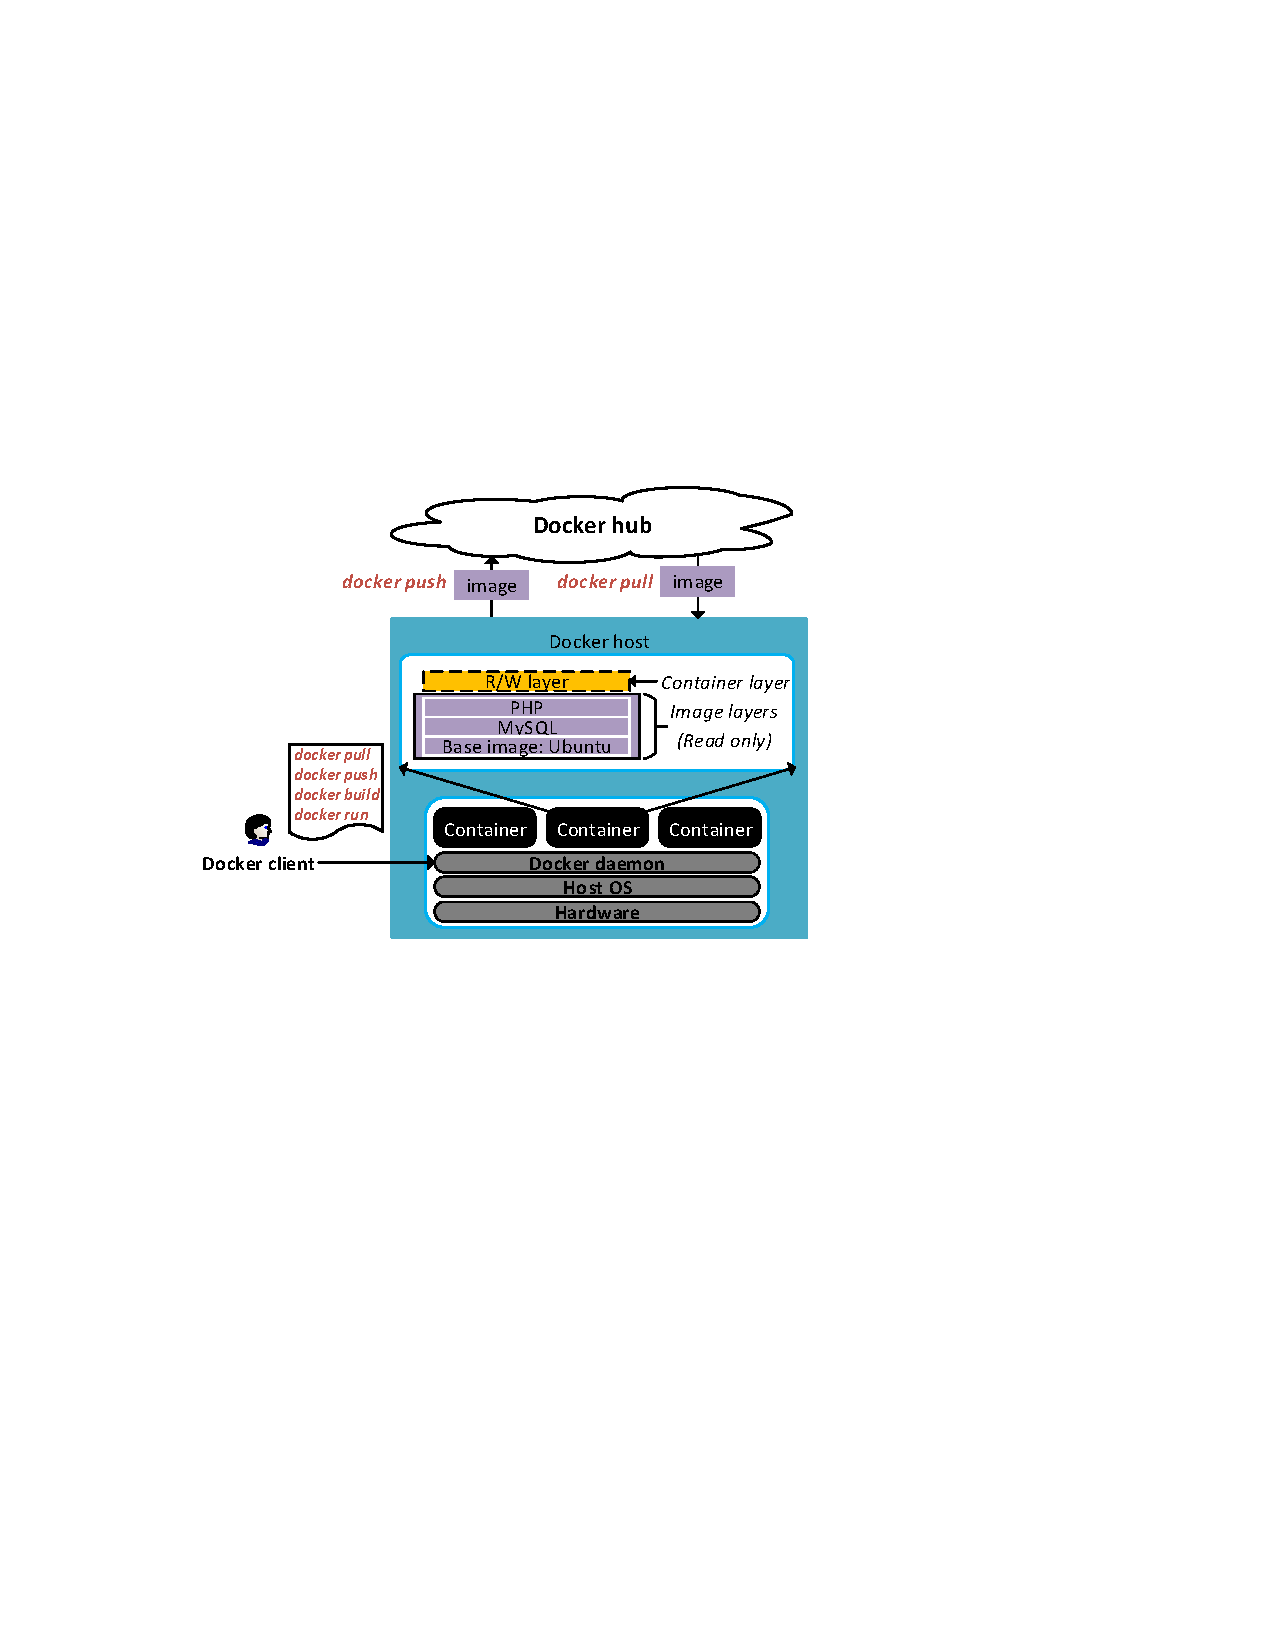
\includegraphics[width=0.5\textwidth]{graphs/fig-docker-architecture}
	\caption{Docker ecosystem
%	\lrcomment{We need to update the figure to capture
%	all the main interactions between the components and remove some unneeded
%	detail, \eg official and unofficial repositories\nancomment{addressed}}
	}
	\label{fig-docker-architecture}
\end{figure}
%
As shown in Figure~\ref{fig-docker-architecture}, a typical
Docker setup consists of three main components: 1)~\emph{client},
2)~\emph{host}, and 3)~\emph{registry}.
%
Users interact with Docker using the Docker client which, in turn,
sends commands to the Docker host.
%
Both client and host can run on the same machine.
%
Docker host runs a daemon process that implements the core logic of Docker and
is responsible for \emph{running} containers from locally available
images.
%
If a user tries to launch a container from an image that is not available
locally, the daemon \emph{pull}s the required image from the Docker registry.
%
Additionally, the daemon supports \emph{building} new images and \emph{pushing}
them to the registry.

\paragraph{Images and layers}
%
At the center of Docker is the concept of container images for packaging,
distributing, and running applications.
%
A Docker image consists of an ordered series of \emph{layers}.
%
Each Docker layer contains a subset of the files in the image and often represents a
specific component/dependency of the image, \eg a shared library.
%
Layers can be shared between two or more images if
the images depend on the same component.

Image layers are read-only.
%
When users start a container, Docker creates a new
\emph{writable layer} on top of the underlying read-only layers
(Figure~\ref{fig-docker-architecture}).
%
Any changes made to files in the image will be reflected inside the writable
layer via a copy-on-write mechanism~\cite{docker-driver-eval}.
%
This leaves layers unmodified throughout the lifetime of a container and
enables layer sharing between multiple containers spawned from the same or
different images.
%
%Docker supports multiple \emph{storage drivers} such as Aufs or Btrfs, which
%efficiently combine read-only and writable layers in a single
%namespace~\cite{docker-driver-eval}.
%
%The writable layers are deleted when the container is deleted.

%Image is represented by a \emph{manifest} which describes the various
%constituents of a Docker image, such as the target hardware platform and
%environment settings.
%%
%Moreover, the manifest contains a list of layer digests for all layers required
%by the image.


\paragraph{Registry}
%
The Docker registry is a platform for storing and sharing container images.
%
It stores images in \emph{repositories}, each containing different versions of
the same image. 
%
For each image Docker registry stores a \emph{manifest} that describes,
among other things, which layers constitute the image.
%
%The manifest is a JSON file, which contains the runtime configuration for a
%container image (\eg target platform and environment variables) and the list
%of layers which make up the image.
%
Layers are identified via a digest that is computed as a hash (SHA-256)
over the layers' uncompressed content and stored as compressed archival files.
%
%Image layers are stored as compressed archival files and image
%manifests as JSON files.
%
%\VT{What is image manifest? Need to introduce}
%
%
%Docker Hub is one of the most popular public registries, supporting both
%public and private repositories, via which users can upload, search, and
%download images~\cite{docker-hub}.
%
%In Docker Hub, the user repositories are namespaced by user name, i.e.,
%``$\langle username\rangle/\langle repository name \rangle$", while the
%official repositories, which are directly provided by Docker Inc. and partners
%are called ``$\langle repository name \rangle$".

%Modern Docker registry identifies and addresses a layer with a digest that is
%computed based on the uncompressed layer's content (e.g., SHA-256).
%
Identifying layers by their content allows the registry to store only one instance
of a layer even if it is referenced by multiple images.
%
\LR{Is that actually done across the entire registry or only within a single
user/repository? \NZ{entire registry}}
%multiple users accidentally built identical layers.
%
However, if at least one file differs in two otherwise identical layers,
the two layers are treated as different and stored separately.

\subsection{Observations and Motivation} % just find the problem and benefit
\label{sec:observationandmotivation}

%\subsection{Need for Deduplication}

%The proliferation of Containers and Container platforms has resulted in an explosion of the number of Docker images.
%In order to understand the extent of storage requirements and performance demands from a Docker registry, 
%we observe the amount of public repositories hosted by Docker Hub registry. 
%We chose the Docker Hub registry~\cite{docker-hub} as our source of images due to its popularity 
%and its significant number of public repositories. 
%%
%Docker Hub does not provide an API to retrieve all repository names.
%Hence, we crawled the registry's website to obtain a list of all available
%repositories, and then downloaded the \emph{latest} version of an image and its
%corresponding layers for each repository.
% over a period of 30 days.
%
%We plan to extend our analysis to other image tags in the future.
%
%We downloaded 355,319 images, resulting in 1,792,609 compressed layers
%and 5,278,465,130 files, with a total compressed dataset size of 47\,TB.
%
%
%To store and analyze the data, we deployed an 8-node Spark~\cite{spark}
%cluster with HDFS~\cite{hdfs} as the backend storage.
%%

\paragraph{Deduplication for Docker registries?}

%\subsection{Deduplication on cloud storage systems}

%Modern Docker registry identifies and addresses a layer with a digest that is computed based on the uncompressed layer's content (e.g., SHA-256).
%Identifying layers by their content allows the registry to store only one instance of a layer even if it is referenced by multiple images. 
%However, if at least one file differs in two otherwise identical layers, the two layers are treated as different and stored separately.
%\paragraph{Images and layers}

We observe that the number of public repositories in Docker Hub is constantly increasing with a growth that amounts 
to around 1 million repositories annually. Based on our estimation, this will cause at least~130\,TB of annual growth in storage needs.

On-cloud global deduplication software is widely adopted by cloud enterprises for reducing cloud storage consumption and overall storage cost. 
For example, StorReduce~\cite{storReduce}, the deduplication software choice of Google cloud and AWS, 
performs in-line data deduplication transparently and resides between the client's application and the hosting cloud storage.
%A number of deduplication methods focus on client-side data deduplication to ensure that only unique files are uploaded, 
%to save network bandwidth, by having the client send a duplicate check request~\cite{xxx}~\cite{xxx}. 
%For example, xxxx\NZ{Hadeel, can you add one example and few relatedwork citation?}. 
Intuitively, such deduplication technique can be leveraged to eliminate redundant data from the Docker image storage system.  
Except, the Docker image dataset is different from the common data stream. 
Docker images are \emph{compressed archival files}.
%Intuitively, registries can be deployed as a proxy cache to host frequently requested layers to speedup image pulls and improve performance 
%while the backend cloud storage can leverage deduplication to save storage space.
%However, there are several unique problems concerning the integration of caching and deduplication to the unique Docker registries workload: \textbf{compressed layers}. 
%We investigate the potential for data reduction in the Docker registry by estimating the efficacy of layer sharing and file-level deduplication.
%We noticed that the number of public repositories is constantly increasing with a growth that amounts 
%to around 1 million repositories annually. 
%This corresponds to~130\,TB of annual growth in storage needs 
%\HA{but it is actually less because of shared layers, right?}, 
%costing around~\$15,000 a month if Google Cloud Storage is used~\cite{GoogleCloudStoragePricing}.
%This growth implies significant benefits to data deduplication. 

We performed an in-depth and empirical analysis of file-level deduplication on container images. 
We analyzed around 47\,TB of compressed Docker images (167\,TB after decompression) collected from Docker Hub. 
%In order to provide insights in terms of the redundancy measure in the image dataset and the benefits of deduplication,
%we have to first decompress the layers included in the images. 
%The decompressed layer comprises a set of files. 
%The total number of files we observed amount to over 5 billion files.
Surprisingly, only around 3\% of the those files are unique while the rest are redundant copies. 
We can save around half of the storage space after removing the duplicate files.

To eliminate these redundant files from the compressed layer files, 
changes must be made to the deduplication method. 
Such changes should recognize the compression formats, perform decompression before feeding the data to a block-level or file-level deduplication process. 
Otherwise, the deduplication ratio would be very low since compressed files have a very low deduplication ratio~\cite{meister2012study}. %"GZip-compressed files deduplication ratio is only 5.7%"
Moreover for restoring a layer, the layer's
containing files should all be fetched from wherever they reside, as they are likely to be scattered across multiple servers, 
and then compressed together, which causes a considerable overhead on pull layer requests performance.

To quantify how much performance overhead caused by using deduplication on Docker registry,
we setup five registry with local file system as their backend storage system,
and implemented the above file-level deduplication with decompression and compression operations.
We replayed IBM registry workload \texttt{dal}~\cite{dockerworkload} 
by sending requests randomly to our five registries and presented average latency 
as shown in Figure~\ref{fig:avg_latency_dedup_nodedup}.
Note that since IBM registry workload \texttt{dal} does not contain real layers, so
we extract layer digest from each request and match it with a layer randomly selected from our dataset.

Without deduplication,
the average latency for requesting a layer is around~2\,s for layers with size less than~50\,MB.
The latency increases to~12\,s when the above deduplication is implemented in the backend storage system.
Furthermore, Docker registry performance drops down dramatically for bigger layers.
We observe that the average latency for requesting layers larger than~50\,MB and smaller than~1\,GB
is around~128\,s. The latency worsens when dedupliation is implemented, with an average around~800\,s.

%\HA{running five registries, replaying dal trace using trace replayer-cite, and since the replayer doesn't use real layers we randomly match the request to our dataset downloaded from docker hub. describe how we got these numbers. for dedup, we simply implemented a decompress/compress + file-level deduplication on backend storage systems, we use a CHT based distributed storage system. Figure~\ref{fig:avg_latency_dedup_nodedup}}
\begin{figure}[t]
	\centering
	%\scriptsize
	\begin{minipage}{0.225\textwidth}
		\centering
		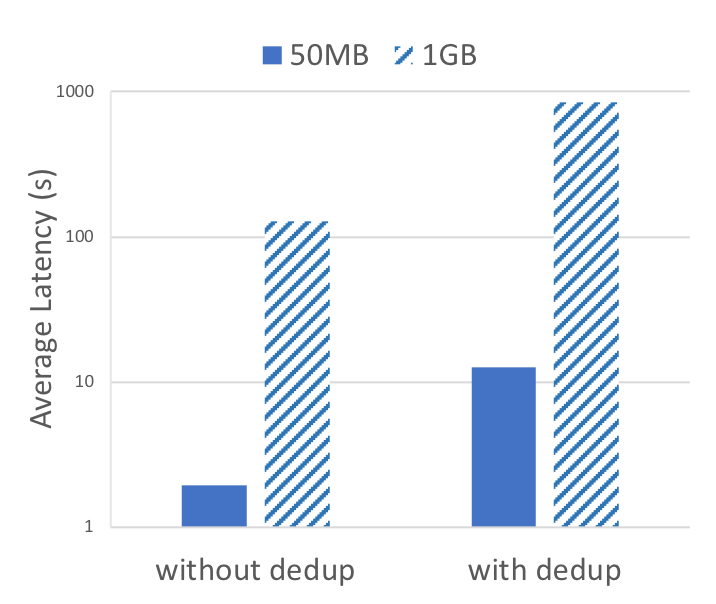
\includegraphics[width=1\textwidth]{graphs/avglatency_dedup_nodedup.png}
		\caption{Average latency.}
		\label{fig:avg_latency_dedup_nodedup}
	\end{minipage}
	\begin{minipage}{0.225\textwidth}
		\centering
		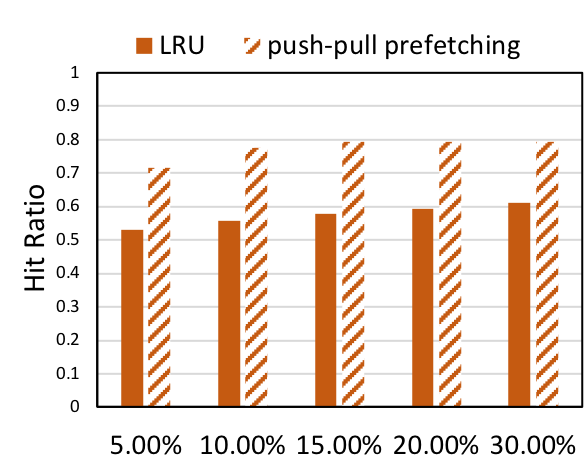
\includegraphics[width=1\textwidth]{graphs/lru_prefetch_hits.png}
		\caption{Hit ratio.}
		\vspace{-3pt}
		\label{fig:lru_prefetching_hits}
	\end{minipage}
\end{figure}
% for LRU and push-pull prefetching under different cache sizes (\% of total accessed layers).

\paragraph{Use registry as a web/proxy cache?}
Traditionally, caches are placed as close to the requesting client as possible, 
such caches are known as proxy caches, or web/HTTP caches for the temporary storage of 
frequently requested data to reduce the remote server lag. 
For example, Varnish~\cite{varnish} and Squid~\cite{squid} are high-performance web/HTTP caches that accelerate web applications and improve response times by caching frequently requested web content.
%Examples of open-source web (HTTP) proxy caches include Nginx~\cite{?}, Squid~\cite{?}, and Varnish~\cite{?}. 
%They are typically implemented in an regional ISP or within a corporate network.
%Deduplication methods are implemented on remote backend storage servers, and
%transparently remove duplicates from the incoming data stream and restore the data for read requests. 
Docker registry is a web server that serves docker \texttt{pull} and docker \texttt{push} requests.
Intuitively, registries can be deployed as a proxy caches, \ie a pull-through cache~\cite{registryascache}, to host frequently requested layers to speedup image pulls and improve performance. 

However, the layer access pattern is largely different from traditional request streams.
Usually, traditional LRU will put recently requested data into cache 
because they will have a big chance to be requested again.
However, it's opposite to layer access pattern: if a layer is pulled by a user,
then this layer mostly will not be pulled in the future by the user 
since this layer is locally available to the user.
Ali Anwar et al. proposed a push-pull prefetch to improve the cache hit ratio~\cite{dockerworkload}.
Based on our following observations, we found the duration between two subsequent layer requests is very long,
if we cache a layer, we might need to wait for hours to get a hit on that layer.

\begin{figure}[t]
	\centering
		\begin{minipage}{0.225\textwidth}
			\centering
			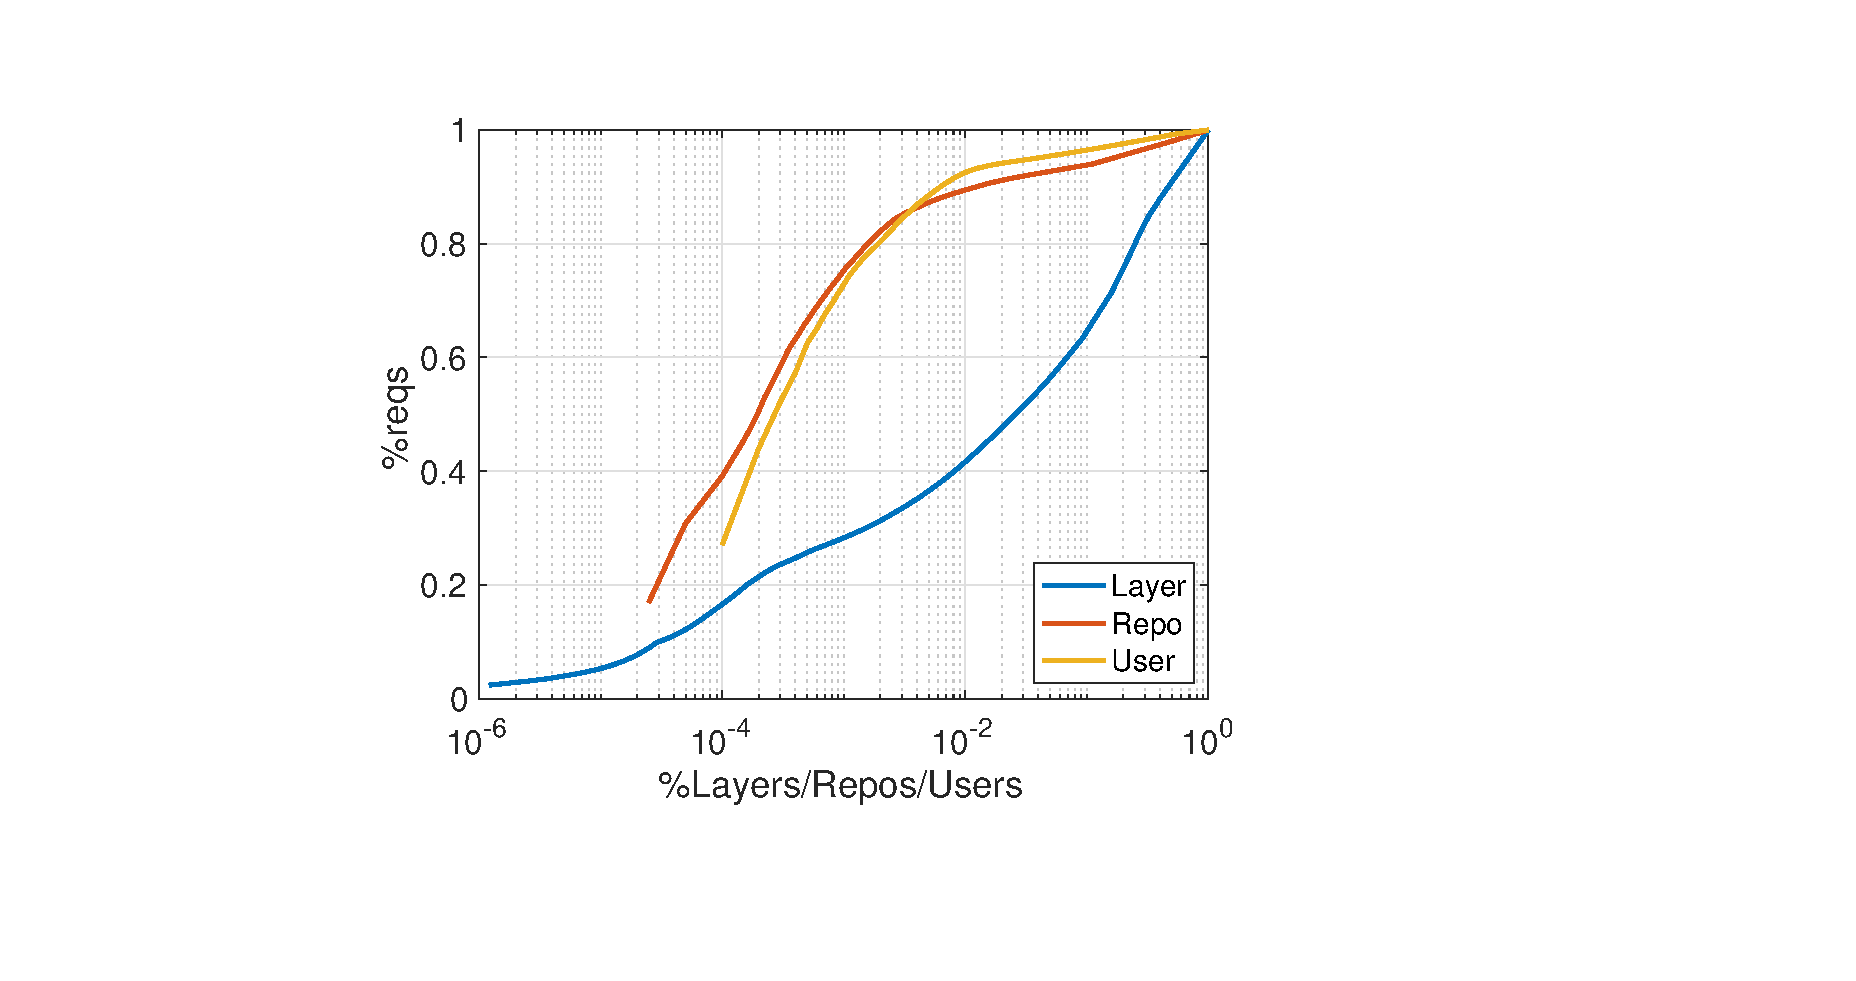
\includegraphics[width=1\textwidth]{graphs/skewness_cdf.eps}
			\caption{Popularity of layers, repos, and users.}
			\label{fig:sknewss}
		\end{minipage}
	\begin{minipage}{0.225\textwidth}
		\centering
		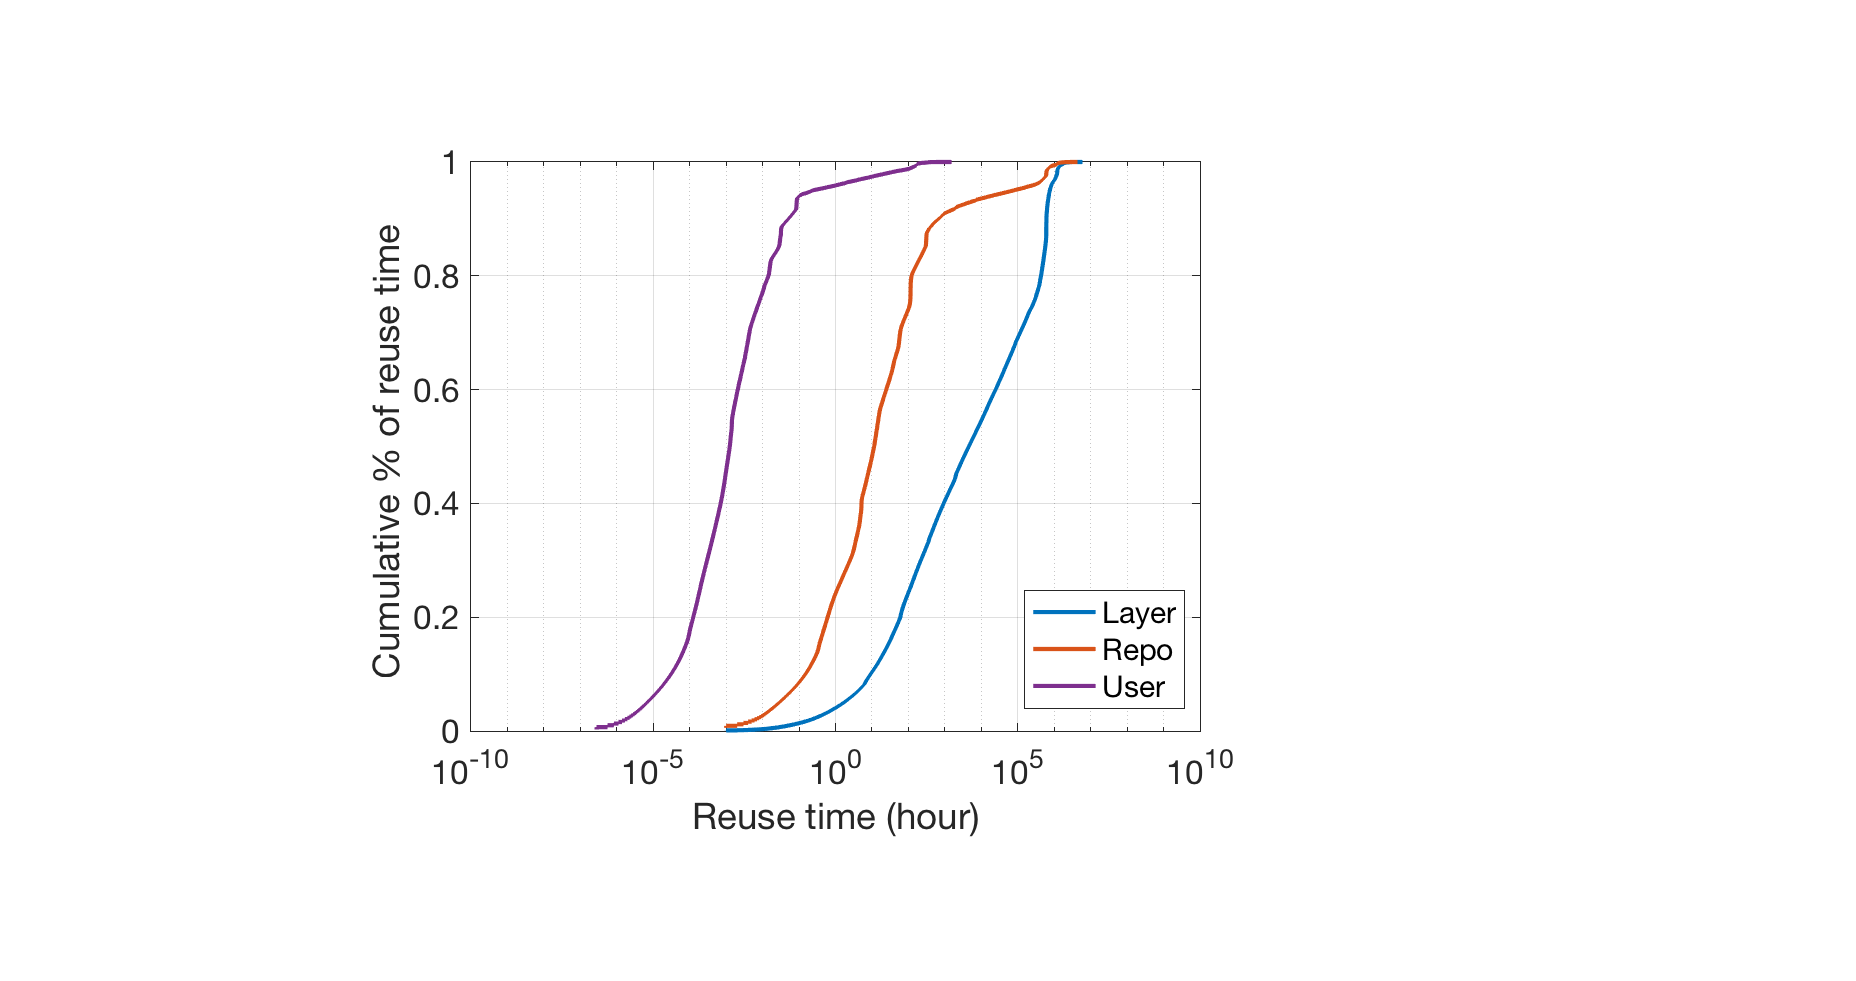
\includegraphics[width=1\textwidth]{graphs/reuse_time.eps}
		\caption{CDF of reuse time for layers, repos, and users.}
		\vspace{-3pt}
		\label{fig:reusetime}
	\end{minipage}
\end{figure}

%\subsection{Observations and motivation} % just find the proble and benefit
%\label{sec:background}
%
%\subsection{Need of Deduplication}
%
%In order to understand the extent of storage requirements and performance demands from a Docker registry. 
%We observe the amount of public repositories hosted by Docker Hub registries. 
%The number of public repositories is constantly increasing with a growth that amounts 
%to around one million repositories annually. 
%This corresponds to~130\,TB of annual growth in storage requirements (but it is acually less because of shared layers, right?), 
%costing around~\$15,000 a month if Google Cloud Storage is used~\cite{GoogleCloudStoragePricing}.
%This growth implies significant benefits to storage deduplication. 
%
%Deduplication option, block level, file level ...?
%
%
%
%\paragraph{Deduplication statistics} % the potiential of deduplication 
%
%how dedup will help
%
%
%layer ref count 
%
%\paragraph{Deduplication ratio growth} % benefit

\subsection{Need for User Behavior based Cache Management}
%\subsection{Need for User behavior based cache management}

%\paragraph{Access skewness}
%According to ~\cite{dockerworkload}, 
%\paragraph{Reuse time distribution}
%\subsubsection{Observations}

%\paragraph{Layers that belong to the same repo have different popularity}
\begin{figure}[t]
	\centering
		\begin{minipage}{0.225\textwidth}
			\centering
			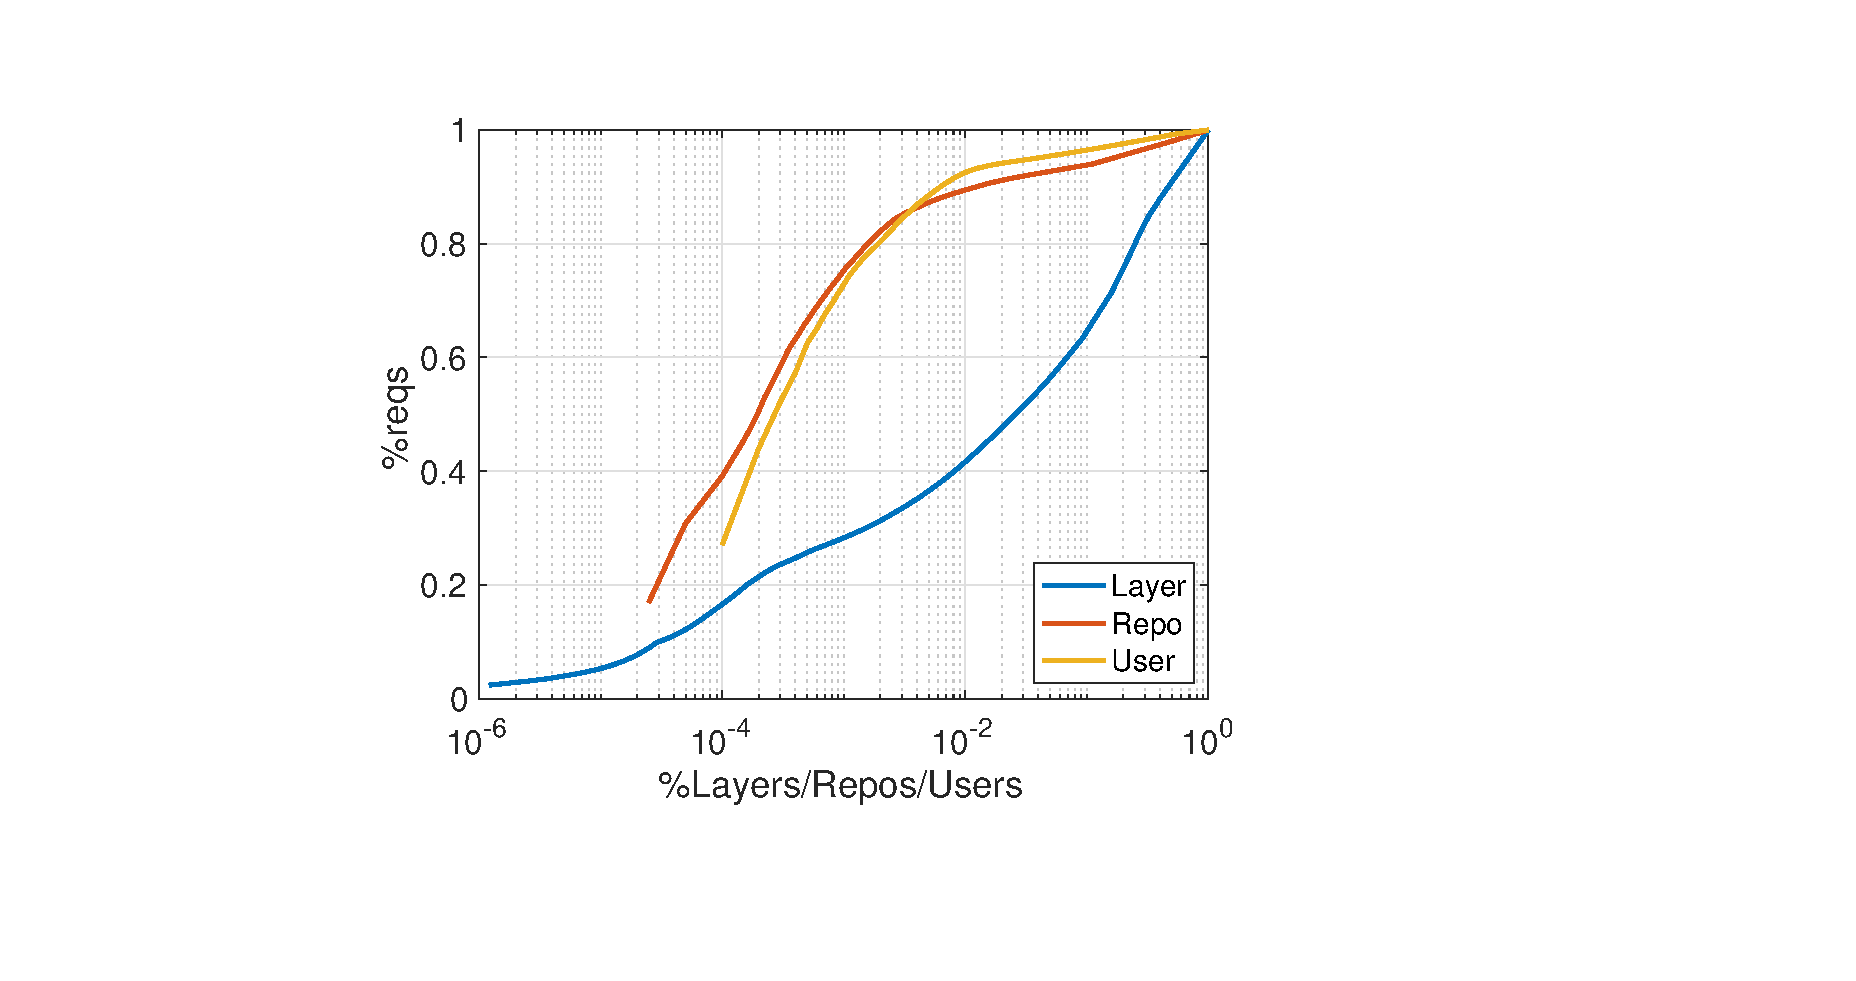
\includegraphics[width=1\textwidth]{graphs/skewness_cdf.eps}
			\caption{Popularity of layers, repos, and users.}
			\label{fig:sknewss}
		\end{minipage}
	\begin{minipage}{0.225\textwidth}
		\centering
		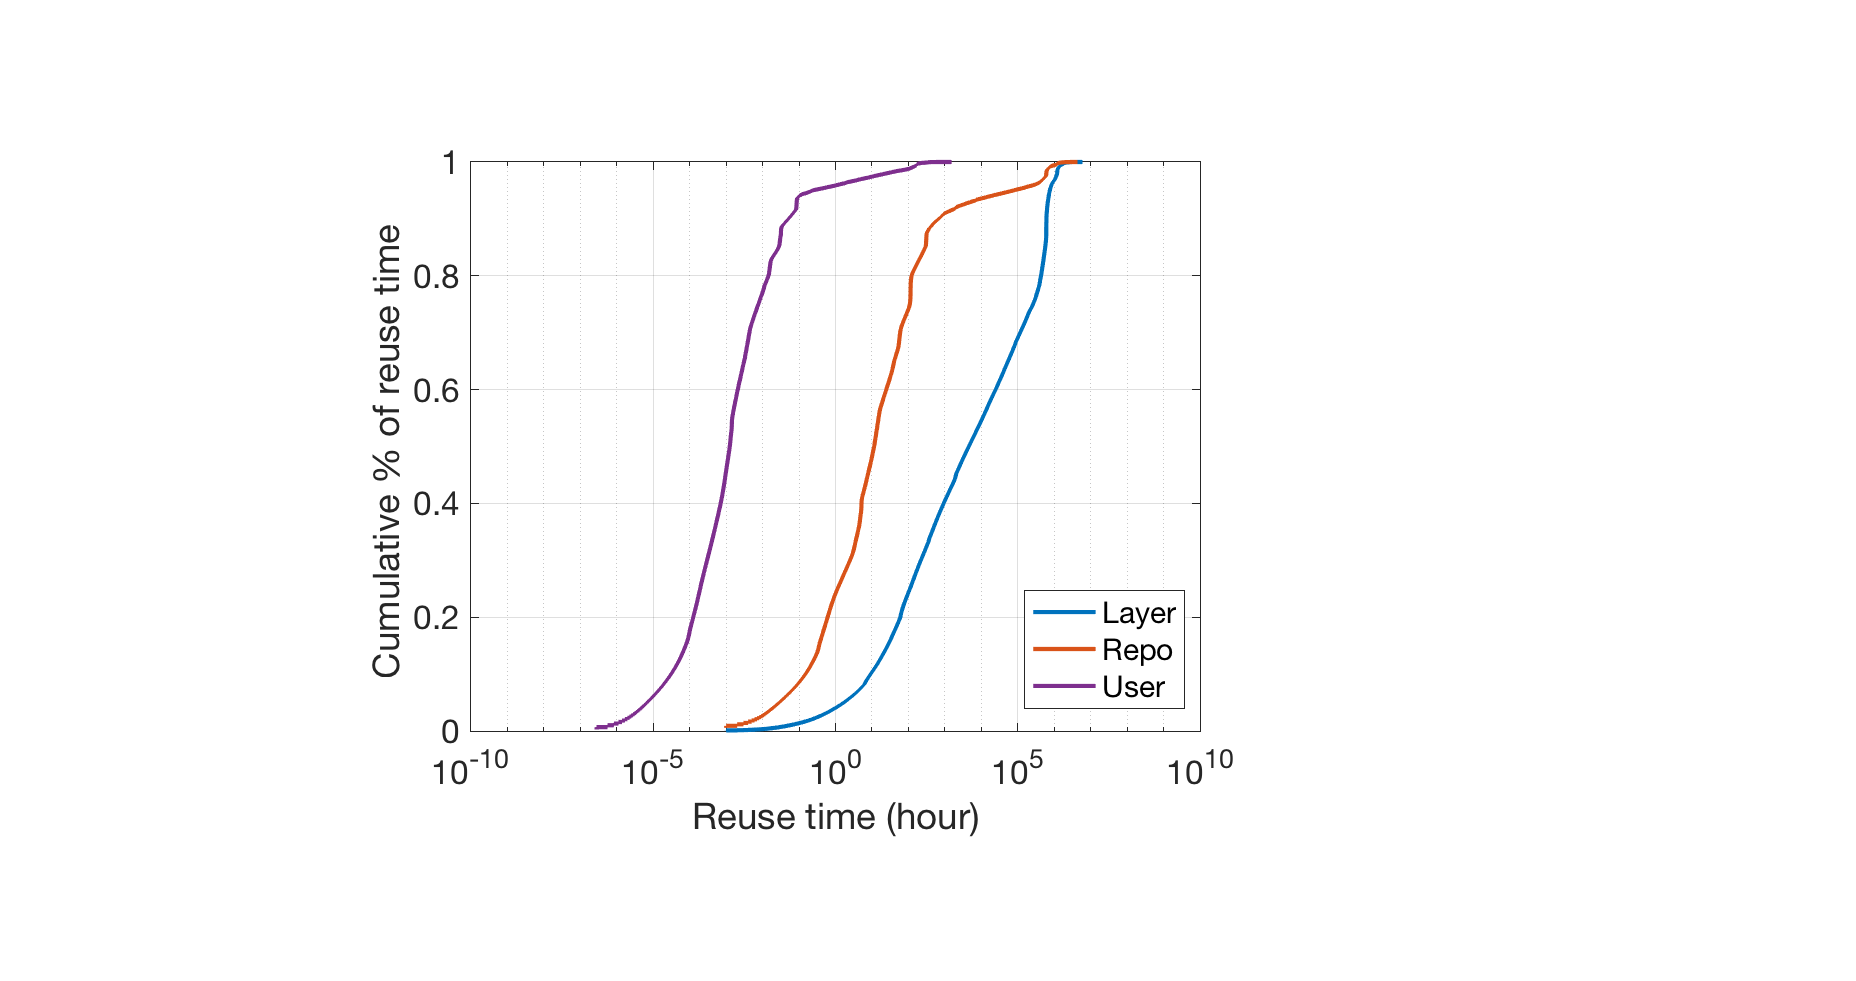
\includegraphics[width=1\textwidth]{graphs/reuse_time.eps}
		\caption{CDF of reuse time for layers, repos, and users.}
		\vspace{-3pt}
		\label{fig:reusetime}
	\end{minipage}
\end{figure}

The following observations are obtained by analyzing the Dallas(\texttt{dal}) registry workload collected from IBM Container Registry over the course of 75 days~\cite{dockerworkload}. 
\paragraph{Requests to layers are heavily skewed but layer reuse time is very long}

Figure~\ref{fig:sknewss} shows the registry accesses to layers and repositories, and accesses by users. 
Layer accesses are heavily skewed. For example, 25\% of popular layers account for 80\% of all requests. 
For repository accesses and accesses by users, the skew is more significant than it is for layers. %10\% most frequently accessed repositories account for 94\% of all requests
94\% of all requests are accessing only 10\% of the most frequently accessed repositories and only 9\% of users, most active ones, issued 97\% of all requests. 
This means that only a few extremely active users create their repositories in the \texttt{dal} registry and issue the majority of requests to the registry.

Figure~\ref{fig:reusetime} shows the reuse time of layers and repositories, and reuse time by users.
Reuse time is the duration between two subsequent requests to access the same layer or repository while 
the reuse time by user is defined as duration between two subsequent requests issued by the same user. 
The layer reuse time is long.
The median reuse time of a layer is 1.3 hours. 80\% of repositories experience the highest request frequency, with a reuse time of around 2 minutes. 
90\% of users remain active for at least 0.06 seconds.
%So for a registry, most of its stored layers are not accessed frequently given a very short time period while
%users can maintain active for a longer time. 
%This is because users can access multiple layers and manifests.
In other words, most of the layers stored in the
registry are not frequently requested in a very short
time period while users remain active for a longer time.
This is because users request different layers or manifests.

\paragraph{User active time is predictable} 
Based on the above observations, we believe that the user's active time is predictable. 
By just maintaining a LRU list of users, we achieved 99\% accuracy for predicting user active time.
For this reason, we utilize this predictability in our cache algorithm.


%We analyzed IBM registry workload and made the two following obervations:
%Caching is a technique widely leveraged to reduce bandwidth and load off of highly loaded bottleneck backends by temporarily storing frequently requested data~\cite{xxx}. 
%Caching can be introduced at the client, in between clients and servers as a proxy, or at the server side. 
%Proxy caches are efficient in reducing traffic from bottleneck backends by cooperatively serving previously requested and saved data without it going all they way to the backend~\cite{xxxx}. 
%Usually, caches are placed as close to the requesting client as possible, 
%such caches are known as proxy caches, or web/HTTP caches for the short-lived storage of 
%frequently requested/accessed data to reduce the server's lag. 

%The client therefore, experiences improved response times.
%The Docker client inherently caches layers at the client. This way, the Docker daemon only pulls layers that are not available on the host machine. 

%Other software used for caching include Memcached~\cite{?}, an open-source distributed in-memory key-value store that works as a caching system and Redis~\cite{?} which is an open-source key-value store that works as an in-memory store and as a cache
%\subsection{Apply traditional deduplication approaches to registries?}
%\subsection{Use-cases of \sysname}
%This suggests that the current layer sharing strategy that Docker already employs is not efficient in eliminating duplicate data. 
%Further investigations on the causes for the high number of redundant files exposed a few findings. 
%For example, different Docker images often contain the same 
%source code from external public repositories like GitHub~\cite{github}.
%This is because no official images contain this source code, 
%so users manually add it to their images, 
%resulting in different layers which cannot be reused.
%\paragraph{Deduplication statistics} % the potential of deduplication 

%%%%layer ref count 
%
%A remarkable observation that emerges from the data analysis is that only around 3\%\HA{3\% or 7\% ?} of the layers' constituent files are unique while the rest are redundant copies. 
%This suggests that the current layer sharing strategy that Docker already employs is not efficient in eliminating duplicate data. 
%We further analyzed the repeat count for every file and plotted the distributions as shown in Figure~\ref{fig:file-repeat-cnt}.
%We found that over 99.4\% of files have more than one copy.
%Around 50\% of files have exactly 4 copies and 90\% of files have 10 or less copies. 
%This indicates the high potential for file-level deduplication in the Docker registry.
%
%%\begin{figure} \centering
%	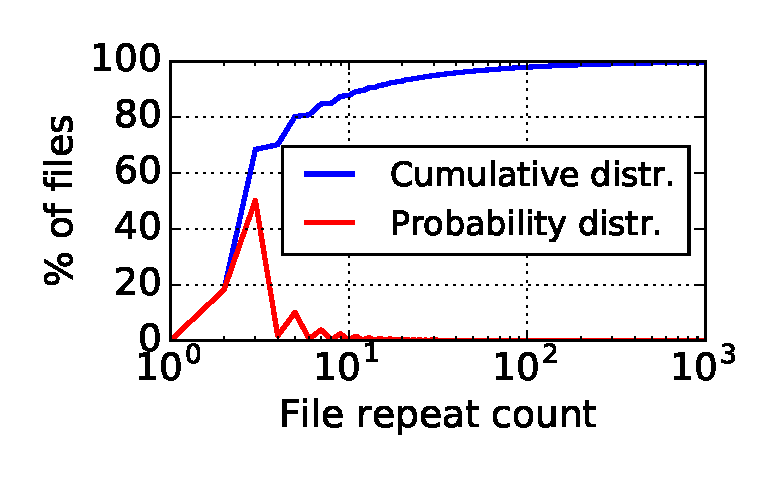
\includegraphics[width=0.45\textwidth]{graphs/File_repeat_count.eps}
%	\caption{File repeat count distribution.
%	%
%	\VT{No need for Y2}
%	%
%	\VT{Still need to use \% on the axis}\NZ{addressed both}
%	%
%	} \label{fig:file-repeat-cnt}
%\end{figure}

\begin{figure}[t]
	\centering
	\begin{minipage}{0.35\textwidth}
		\centering
		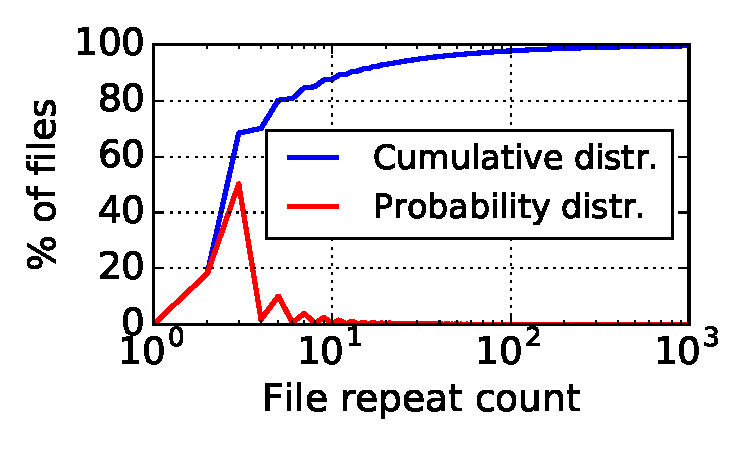
\includegraphics[width=1\textwidth]{graphs/File_repeat_count-eps.pdf}
		\caption{File repeat count distribution.
		}
		%\vspace{15pt}
		\label{fig:file-repeat-cnt}
	\end{minipage}
	\begin{minipage}{0.35\textwidth}
		\centering
		%\vspace{-10pt}
		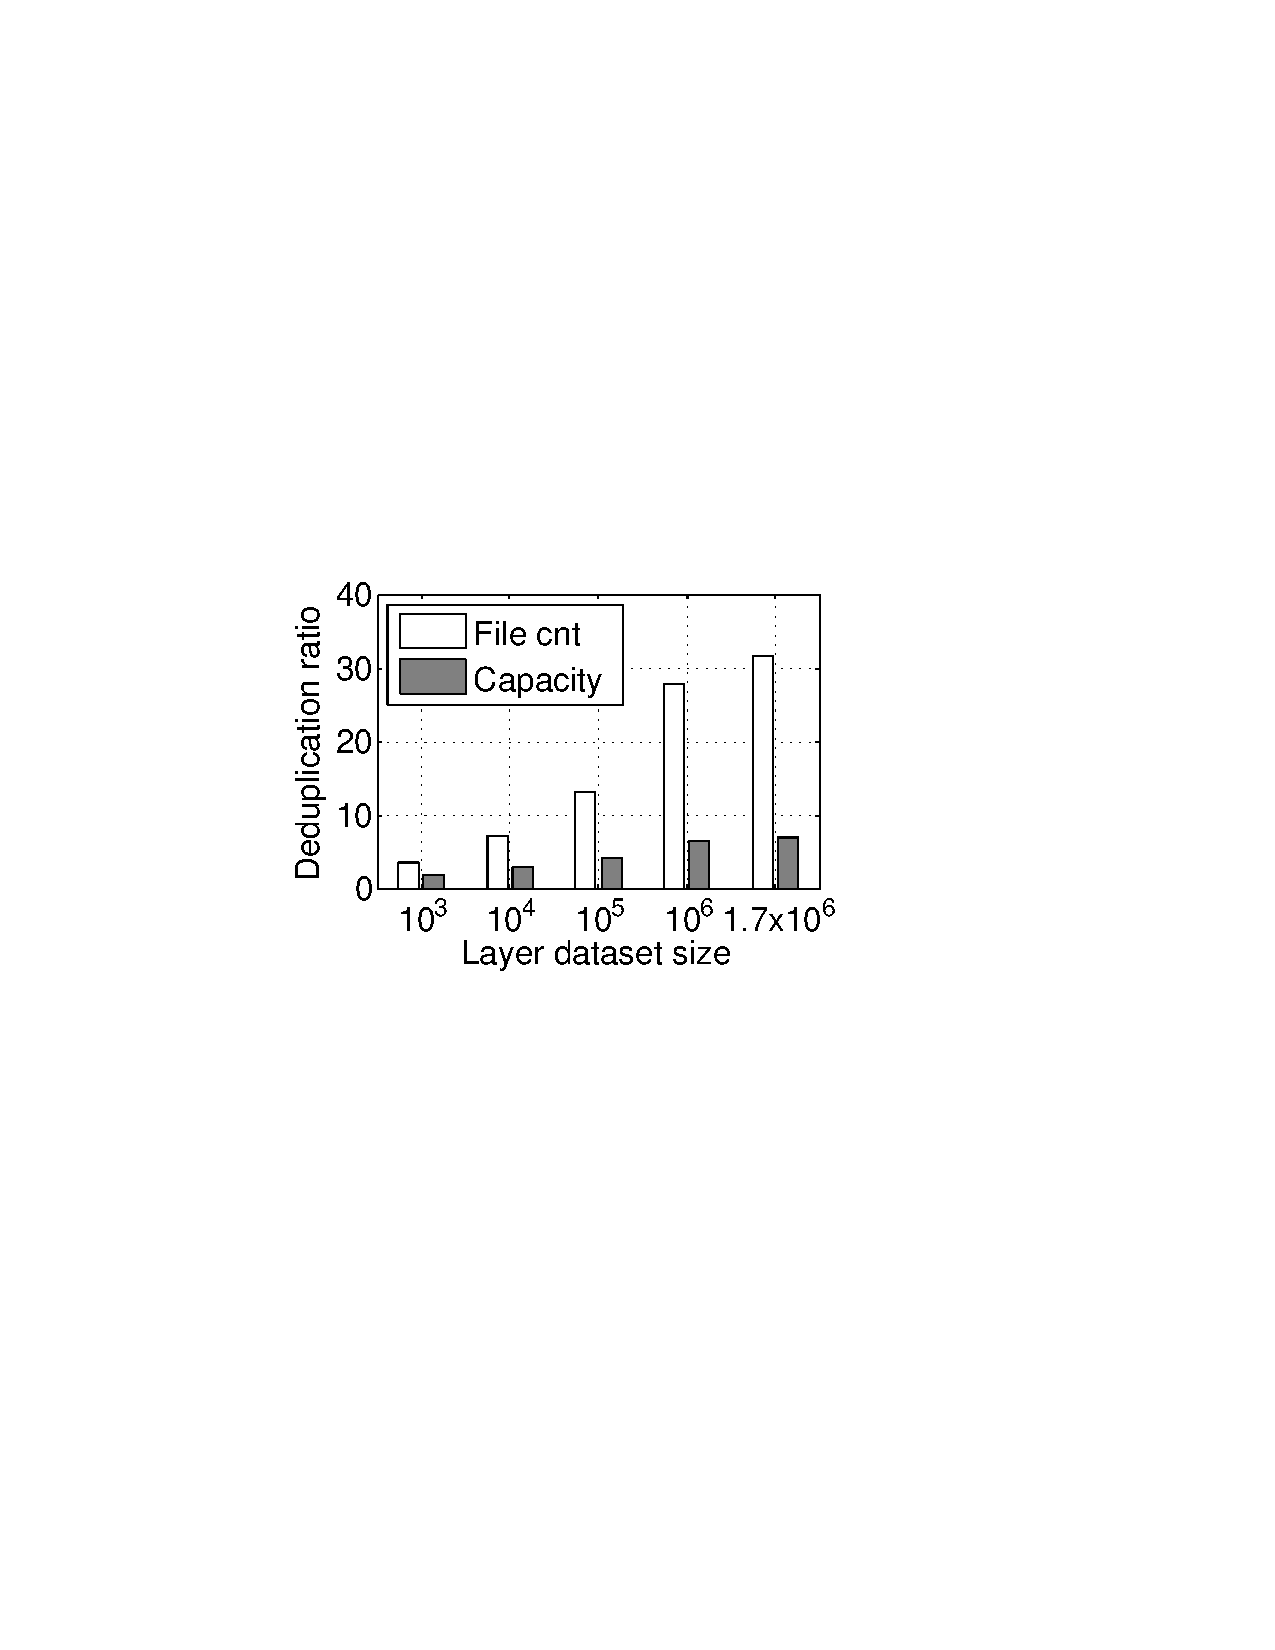
\includegraphics[width=1\textwidth]{graphs/dedup-ratio-grow} 
		\caption{Deduplication ratio growth.
		} 
		\vspace{-2pt}
		\label{fig:dedup-ratio-growth}
	\end{minipage}
\end{figure}

%\begin{figure} 
%	\centering
%	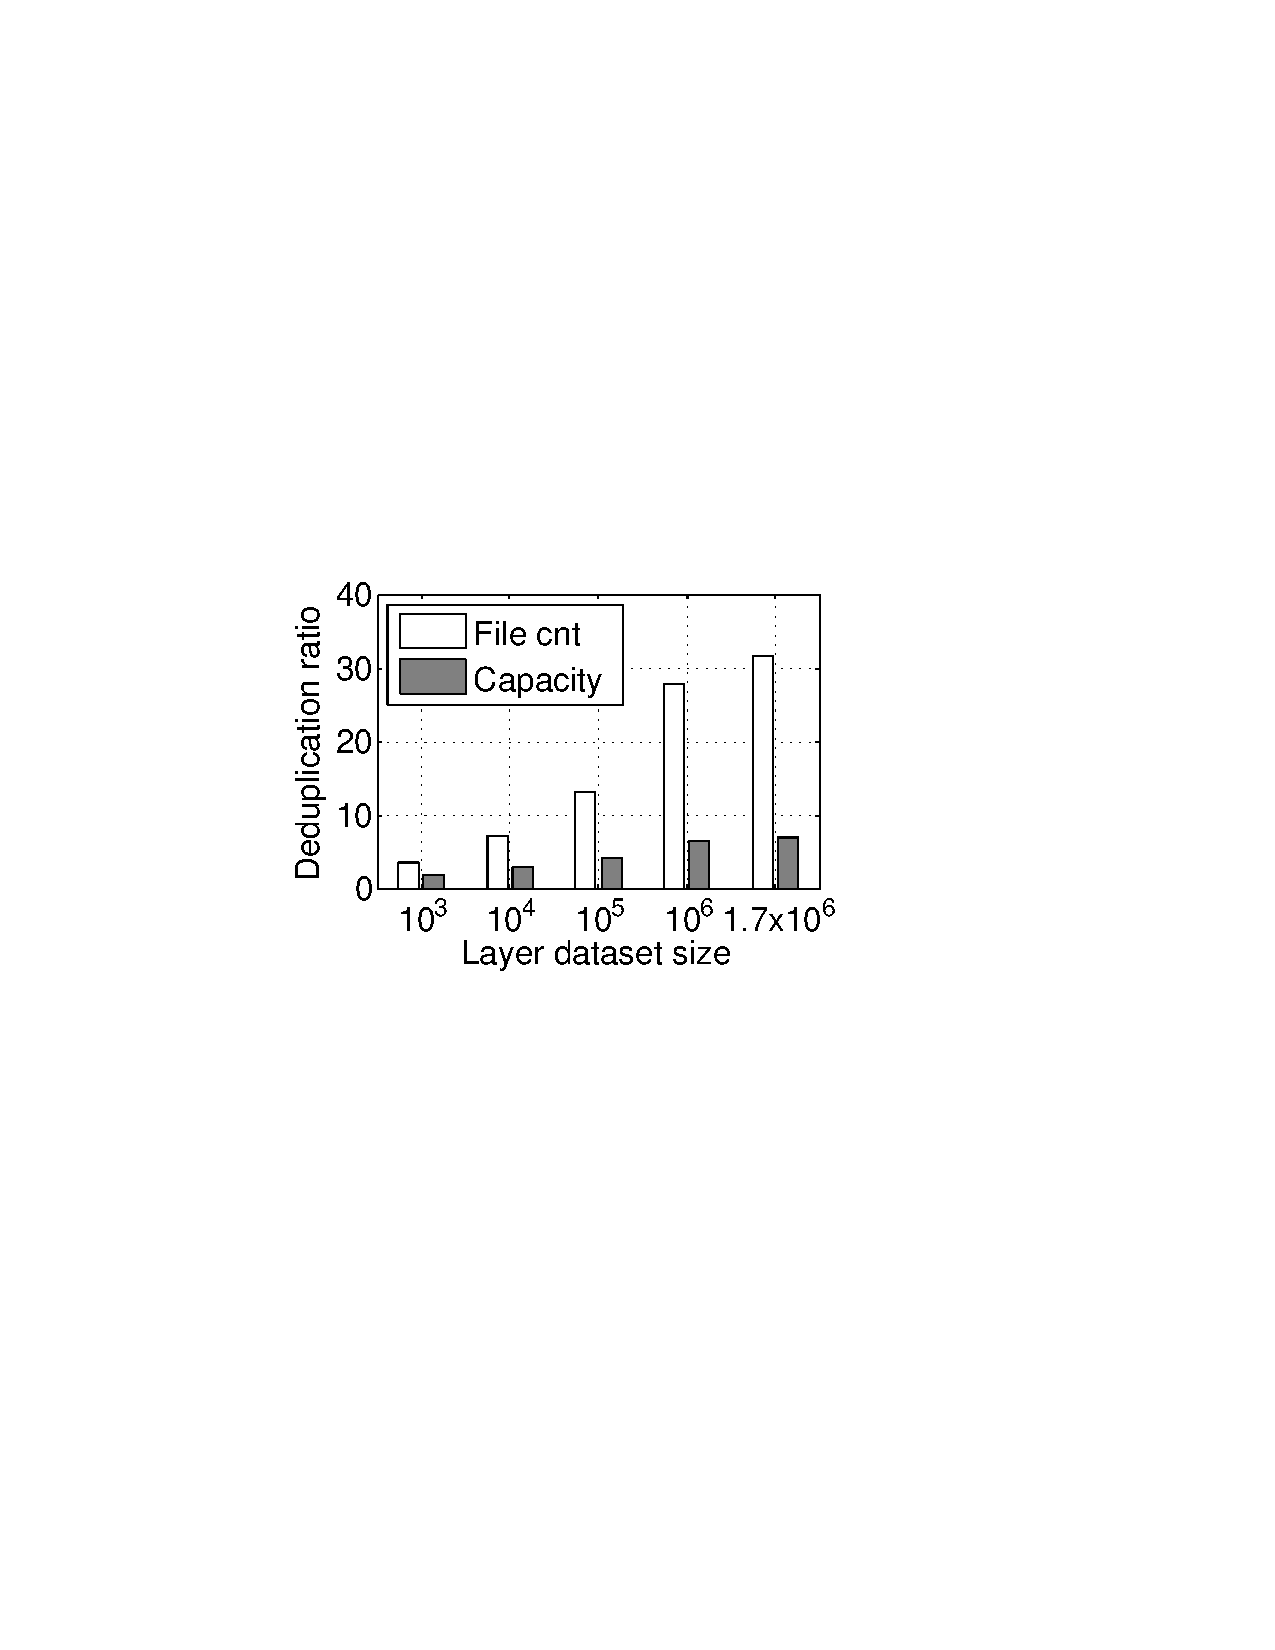
\includegraphics[width=0.25\textwidth]{graphs/dedup-ratio-grow} 
%	\caption{The growth of deduplication ratio.
%	} 
%	\label{fig:dedup-ratio-growth} 
%\end{figure}

%
%
%\paragraph{Deduplication ratio growth} % benefit
%%
%Further investigations on the potential of file-level deduplication involved analyzing the deduplication ratio. 
%As shown in Figure~\ref{fig:dedup-ratio-growth}, we analyzed the deduplication 
%ratio and its growth for an increasing number of files stored in the registry.   
%%(see Figure~\ref{fig:dedup-ratio-growth}).
%%
%%Figure~\ref{fig:dedup-ratio-growth} shows the deduplication ratio growth over the layer dataset size. 
%%
%The x-axis values correspond to the sizes of 4 random samples drawn from the whole dataset and the size of the
%whole dataset.
%
%We see that the deduplication ratio increases almost linearly with the layer dataset size.
%This implies that the benefits of file-level deduplication strengthens as the number of public repositories and images grow.
%
%As the number of images stored in the Docker registry increases dramatically,
%file-level deduplication can provide significant storage space savings.

%Intuitively, registries can be deployed as a proxy cache to host frequently requested layers to speedup image pulls and improve performance 
%while the backend cloud storage can leverage deduplication to save storage space.
%However, there are several unique problems concerning the integration of caching and deduplication to the unique Docker registries workload: \textbf{compressed layers}. 

%\subsection{Need for Usr-oriented cache management}
%
%\paragraph{Access skewness}
%
%\paragraph{Reuse time distribution}
%
%\paragraph{Hit ratios}
%
%\paragraph{Hit ratios with prefetching}
%
%%\subsection{} % what are the cost for a naive file-level deduplication
%
%\paragraph{Restoring performance breakdown}
%\subsection{Observations and motivation} % just find the proble and benefit
%\label{sec:background}
%
%\subsection{Need of Deduplication}
%
%In order to understand the extent of storage requirements and performance demands from a Docker registry. 
%We observe the amount of public repositories hosted by Docker Hub registries. 
%The number of public repositories is constantly increasing with a growth that amounts 
%to around one million repositories annually. 
%This corresponds to~130\,TB of annual growth in storage requirements (but it is acually less because of shared layers, right?), 
%costing around~\$15,000 a month if Google Cloud Storage is used~\cite{GoogleCloudStoragePricing}.
%This growth implies significant benefits to storage deduplication. 
%
%Deduplication option, block level, file level ...?
%
%
%
%\paragraph{Deduplication statistics} % the potiential of deduplication 
%
%how dedup will help
%
%
%layer ref count 
%
%\paragraph{Deduplication ratio growth} % benefit

\subsection{Need for User Behavior based Cache Management}
%\subsection{Need for User behavior based cache management}

%\paragraph{Access skewness}
%According to ~\cite{dockerworkload}, 
%\paragraph{Reuse time distribution}
%\subsubsection{Observations}

%\paragraph{Layers that belong to the same repo have different popularity}
\begin{figure}[t]
	\centering
		\begin{minipage}{0.225\textwidth}
			\centering
			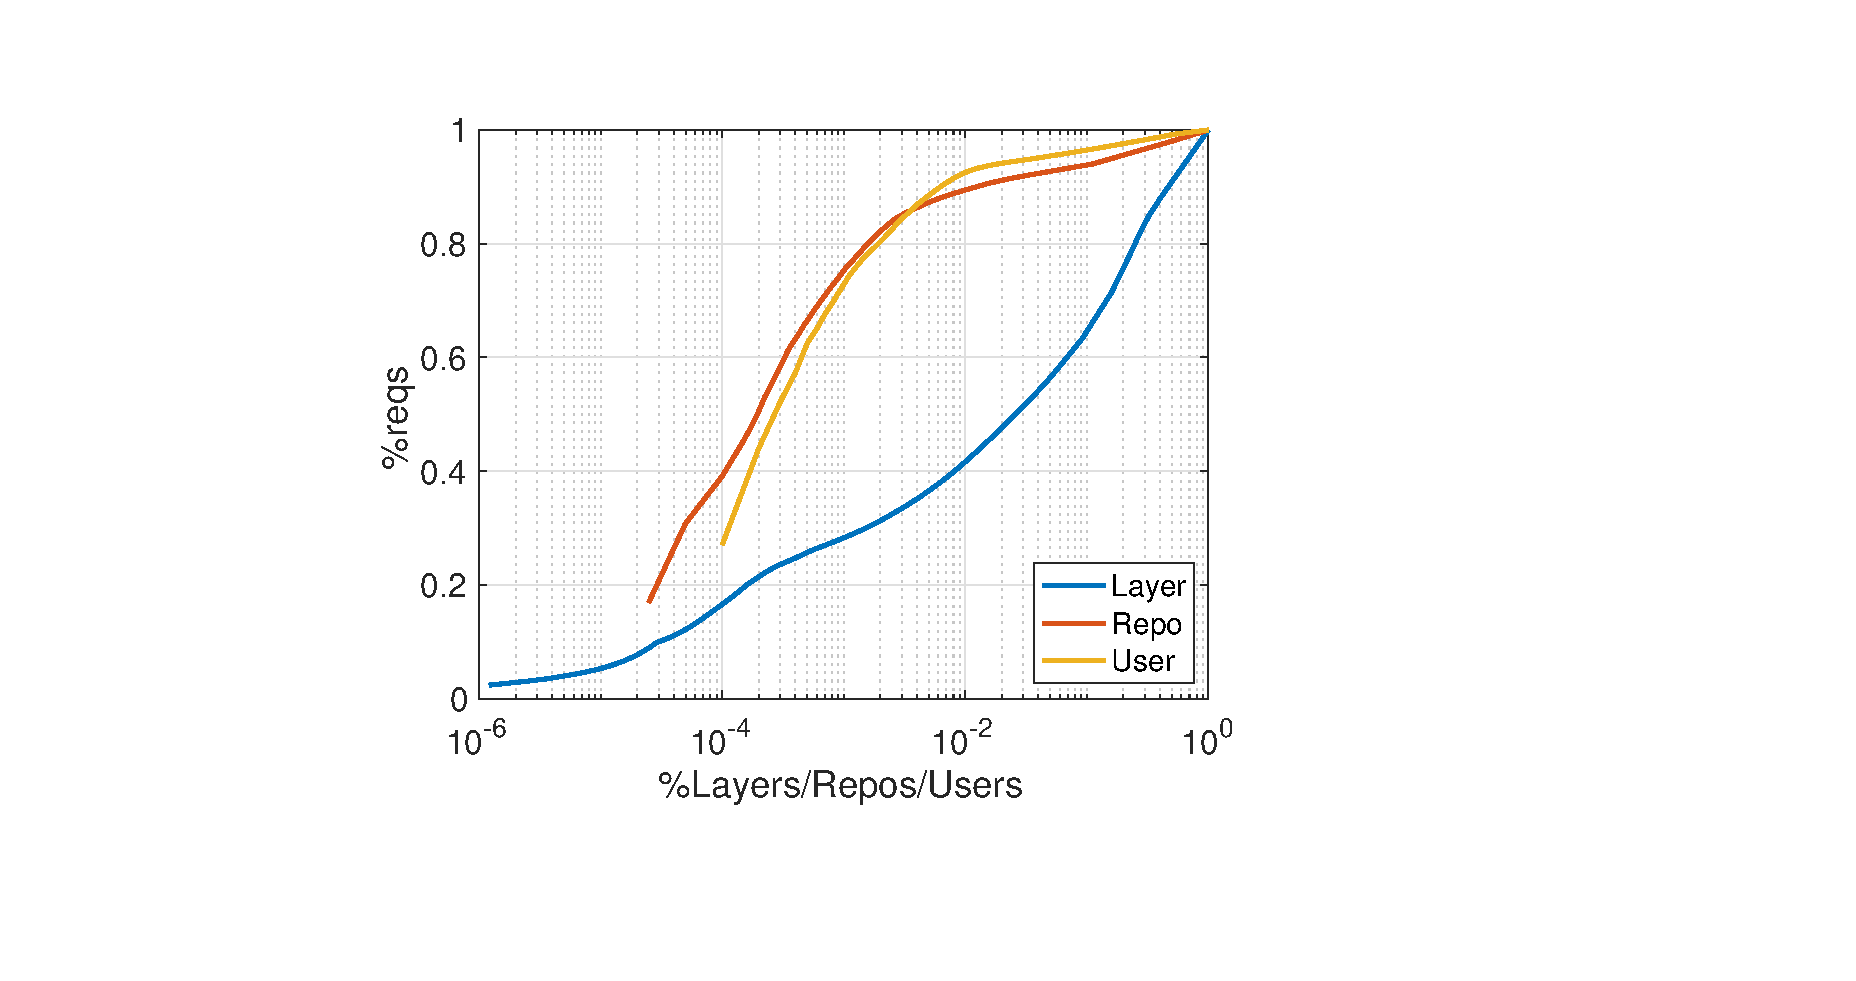
\includegraphics[width=1\textwidth]{graphs/skewness_cdf.eps}
			\caption{Popularity of layers, repos, and users.}
			\label{fig:sknewss}
		\end{minipage}
	\begin{minipage}{0.225\textwidth}
		\centering
		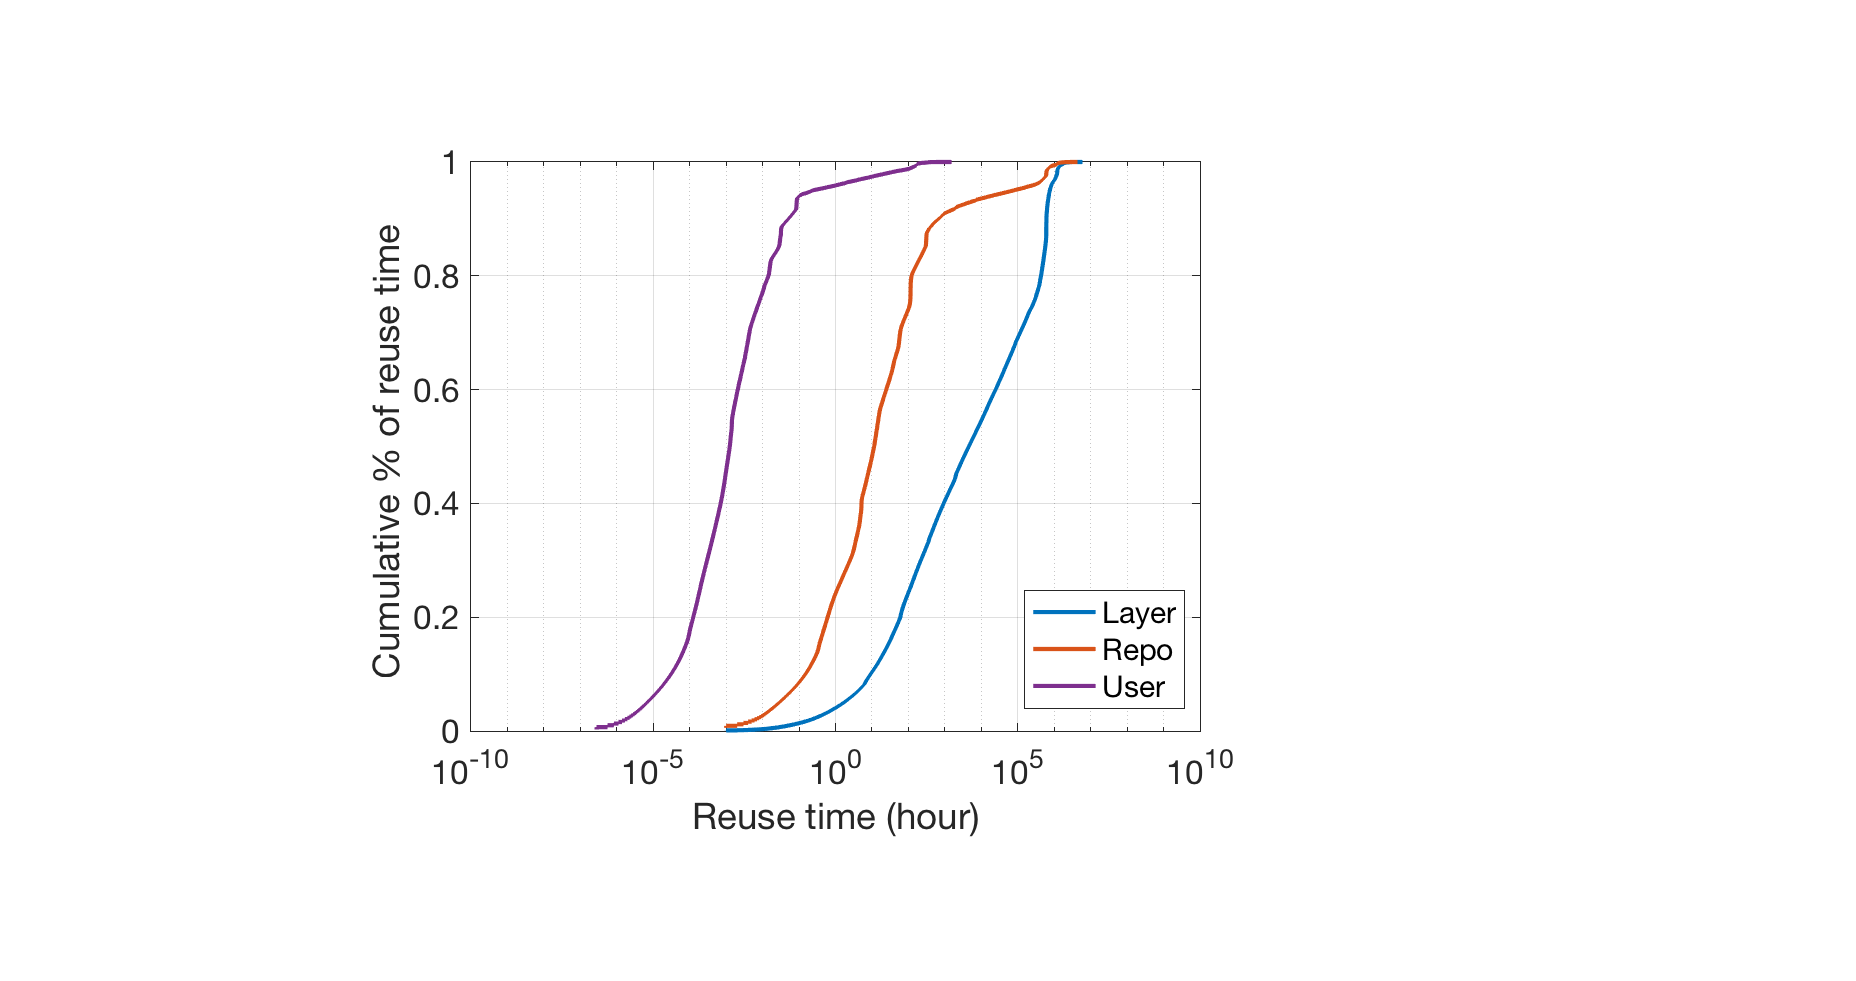
\includegraphics[width=1\textwidth]{graphs/reuse_time.eps}
		\caption{CDF of reuse time for layers, repos, and users.}
		\vspace{-3pt}
		\label{fig:reusetime}
	\end{minipage}
\end{figure}

The following observations are obtained by analyzing the Dallas(\texttt{dal}) registry workload collected from IBM Container Registry over the course of 75 days~\cite{dockerworkload}. 
\paragraph{Requests to layers are heavily skewed but layer reuse time is very long}

Figure~\ref{fig:sknewss} shows the registry accesses to layers and repositories, and accesses by users. 
Layer accesses are heavily skewed. For example, 25\% of popular layers account for 80\% of all requests. 
For repository accesses and accesses by users, the skew is more significant than it is for layers. %10\% most frequently accessed repositories account for 94\% of all requests
94\% of all requests are accessing only 10\% of the most frequently accessed repositories and only 9\% of users, most active ones, issued 97\% of all requests. 
This means that only a few extremely active users create their repositories in the \texttt{dal} registry and issue the majority of requests to the registry.

Figure~\ref{fig:reusetime} shows the reuse time of layers and repositories, and reuse time by users.
Reuse time is the duration between two subsequent requests to access the same layer or repository while 
the reuse time by user is defined as duration between two subsequent requests issued by the same user. 
The layer reuse time is long.
The median reuse time of a layer is 1.3 hours. 80\% of repositories experience the highest request frequency, with a reuse time of around 2 minutes. 
90\% of users remain active for at least 0.06 seconds.
%So for a registry, most of its stored layers are not accessed frequently given a very short time period while
%users can maintain active for a longer time. 
%This is because users can access multiple layers and manifests.
In other words, most of the layers stored in the
registry are not frequently requested in a very short
time period while users remain active for a longer time.
This is because users request different layers or manifests.

\paragraph{User active time is predictable} 
Based on the above observations, we believe that the user's active time is predictable. 
By just maintaining a LRU list of users, we achieved 99\% accuracy for predicting user active time.
For this reason, we utilize this predictability in our cache algorithm.



%\section{Image, layer, and file characterization}
\label{sec:char}

In this section we carry out our analysis of the Docker Hub dataset by characterizing
layers and images based on
the presented metrics. While overall we are interested in its general structure,
we also analyze specific properties that allow us to draw conclusions regarding the
caching, compression, and resource provisioning.

%In this section, we present comprehensive characterization of Docker images and
%layers.  We analyze and present the highlights of dataset stored by Docker Hub
%registry.  We also provide useful insights (parameters or metrics)
%for the developers to better
%understand the file systems used by Docker container.  

\subsection{Layers}
\label{sec:layers}

%\nancomment{could remove archival size from all sections}
We start by analyzing layers in terms of size and compressibility, and file and directory
counts and directory depths.

%%%%%%%%%%%%%%%%%%%%%%%%%%%%%%%%%%%%%%%%%%%%%%%%%%%%%%%%%%%%%%%%%%%%%

\begin{figure}[!t]
	\centering
	\subfigure[CDF of layer sizes]{\label{fig_layer_size_cdf}
		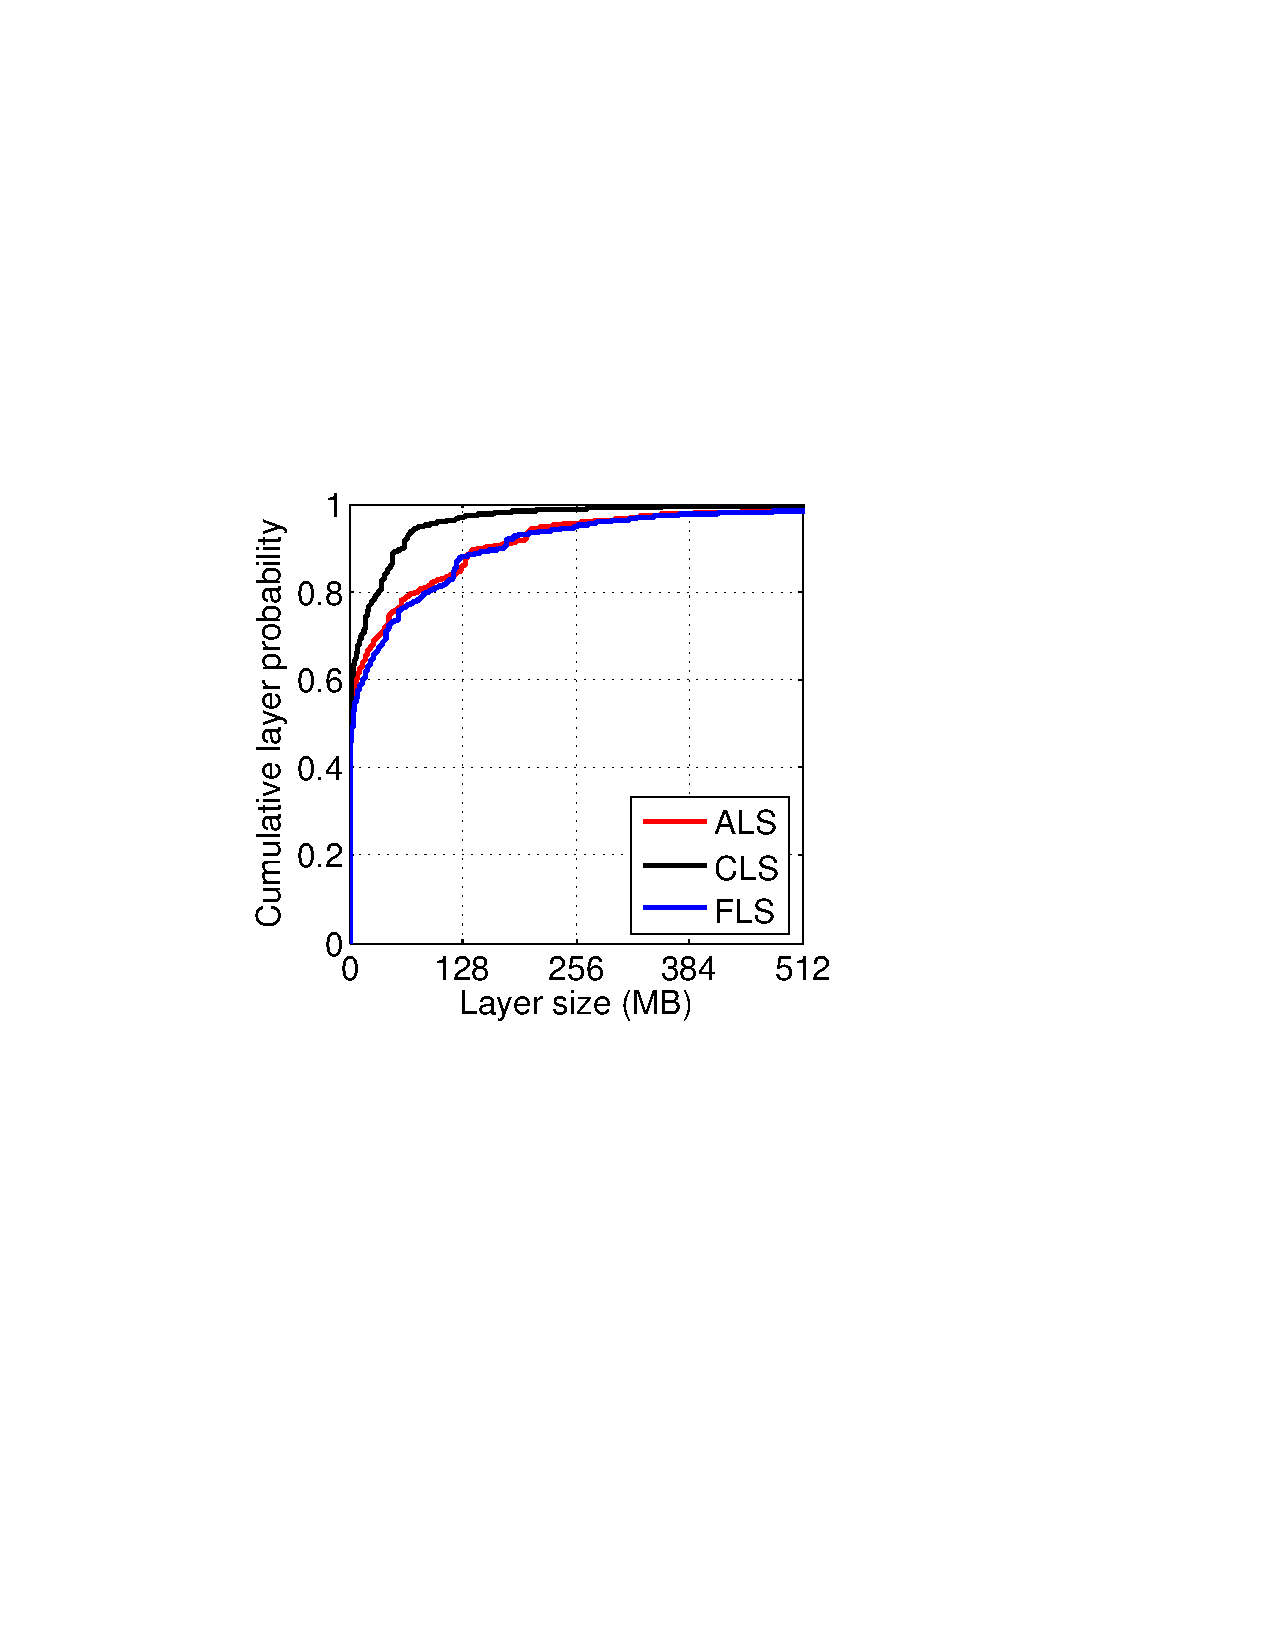
\includegraphics[width=0.234\textwidth]{graphs/layer_size_mb.pdf}
	}
	\subfigure[Histogram of layer sizes]{\label{fig_hist_layer_size}
		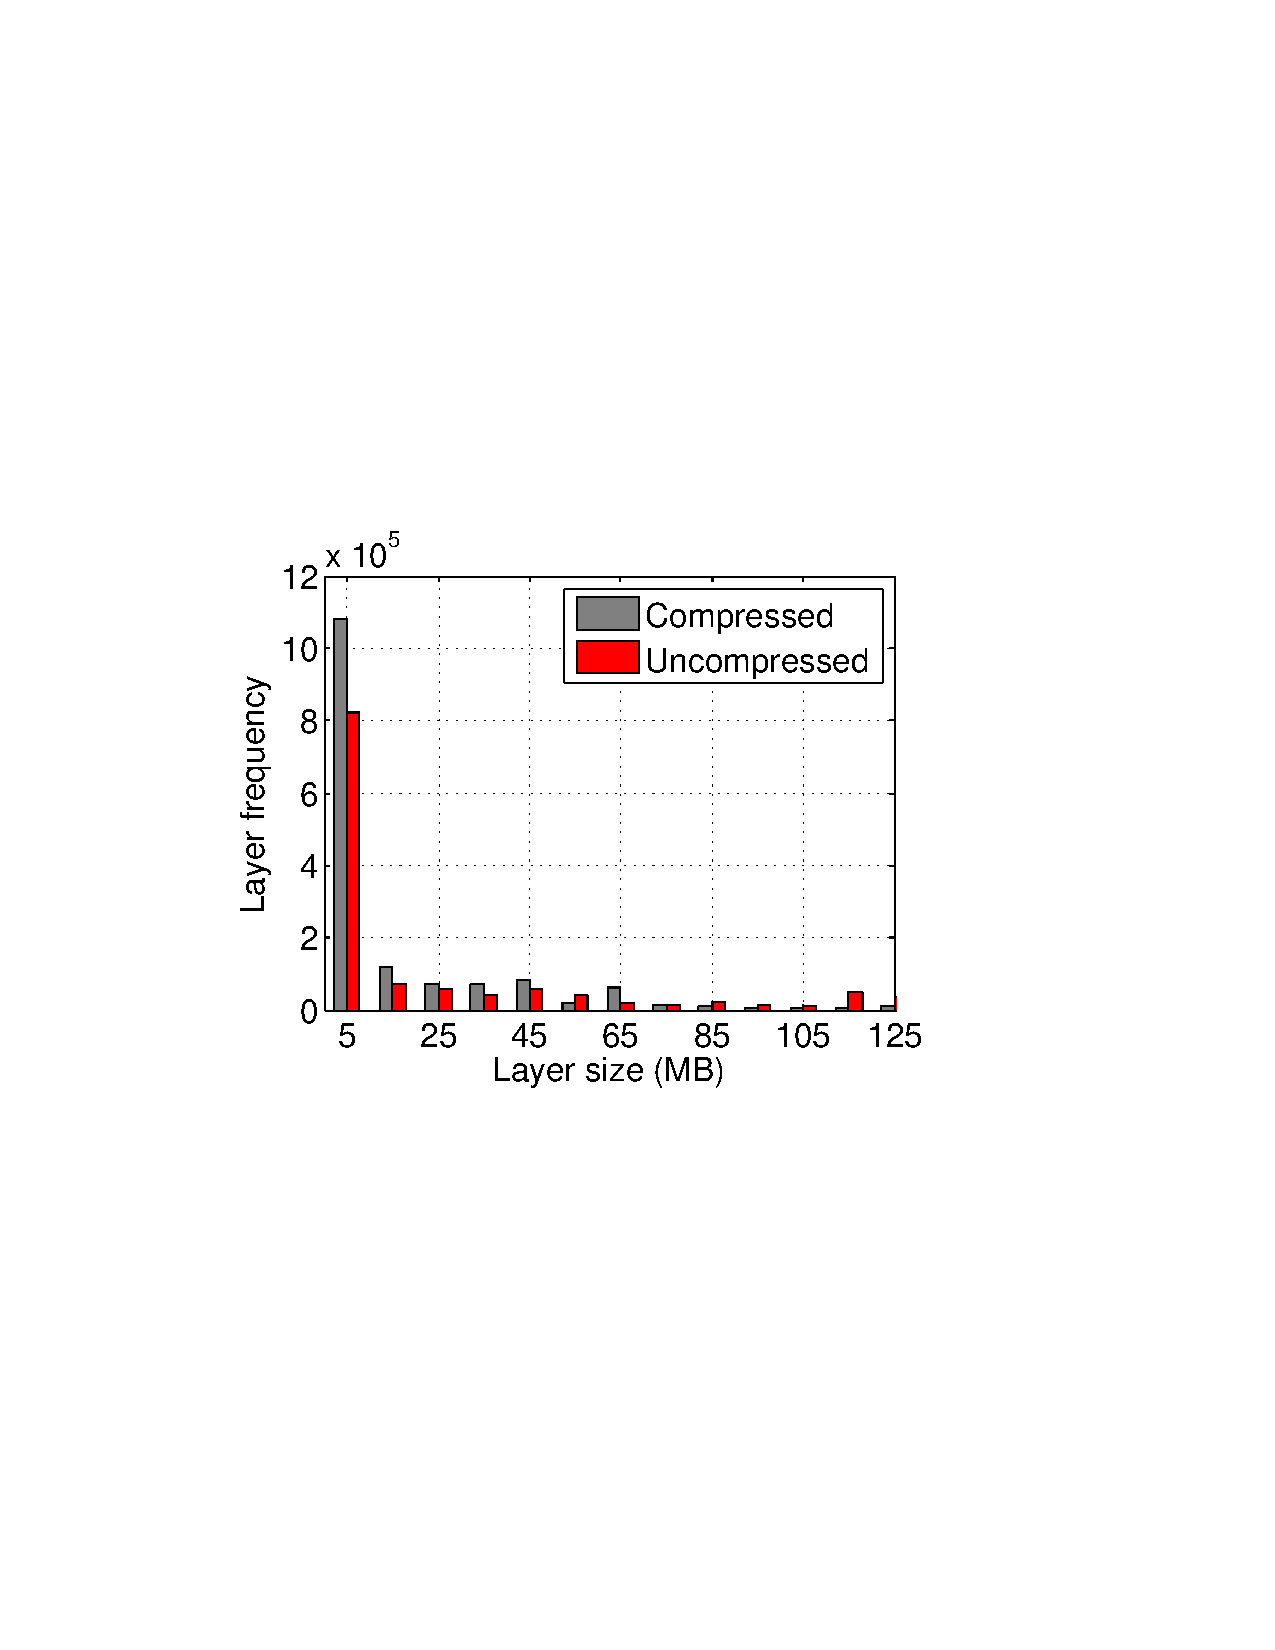
\includegraphics[width=0.213\textwidth]{graphs/hist_layer_size.pdf}
	}
	\caption{Layer size distribution
	\vcomment{Let's use CLS, ALS, and FLS abreviations\nancomment{addressed}}.
	\vcomment{CLS size should go first}.
	\vcomment{We need to use different types of lines (solid, dotted, etc.)
		or markers (round, triangular)}.
	\vcomment{In figure B it is not clear to which bar group corresponds
		  to which layer size. I suggest to try to rotate the graph
		  by 90 grads to fit all layer size labels.\nancomment{aligned label with bar}}
	}
	\label{fig-layer-size}
\end{figure}


\paragraph{Layer sizes}
%
We characterize layer sizes using two different different metrics:
%
1)~Compressed Layer Size (CLS)---the format a layer is stored in the registry or
transferred to a client;
%
%2)~Archived Layer Size (ALS)---layer in decompressed but archived format;
%
and 2)~Files in Layer Size (FLS)---the sum of the size of the uncompressed files contained
in the layer.
%
Figure~\ref{fig_layer_size_cdf} shows the CDF of the two metrics.


%The ALS and FLS curves are, expectedly, close to each other (within 5\% for
%any given layer size) while compressed layers are typically smaller.
%j
We see that 90\% of the layers are smaller than 177~MB in uncompressed 
format and smaller than 63~MB in compressed format.
%
Interestingly, about half of the layers are smaller than 4~MB, independent
of the format. That means that the registry stores a large number of
small layers which cannot benefit from compression.
%
\nancomment{I removed the following lines because we analyzed all layers.}
%As we described earlier in \S~\ref{sec:methodology}, we only
%analyzed layers smaller than 2~GB in compressed format. This
%resulted in the largest analyzed uncompressed layer being
%of \gap~GB large.
%
%\vcomment{need to adjust Methodology to reflect this.}

To analyze the actual numbers, we zoom into the 0--128~MB range
(see Figure~\ref{fig_hist_layer_size}).
%
More than 1 million and 800,000 layers are smaller than 5~MB
in compressed and uncompressed format, respectively. After that,
the frequency drops rapidly and we only see around 100,000 layers
between 5~MB and 15~MB.

\begin{figure}[!t]
	\centering
	\subfigure[CDF of compression ratio]{\label{fig_cdf_compression_ratio}
		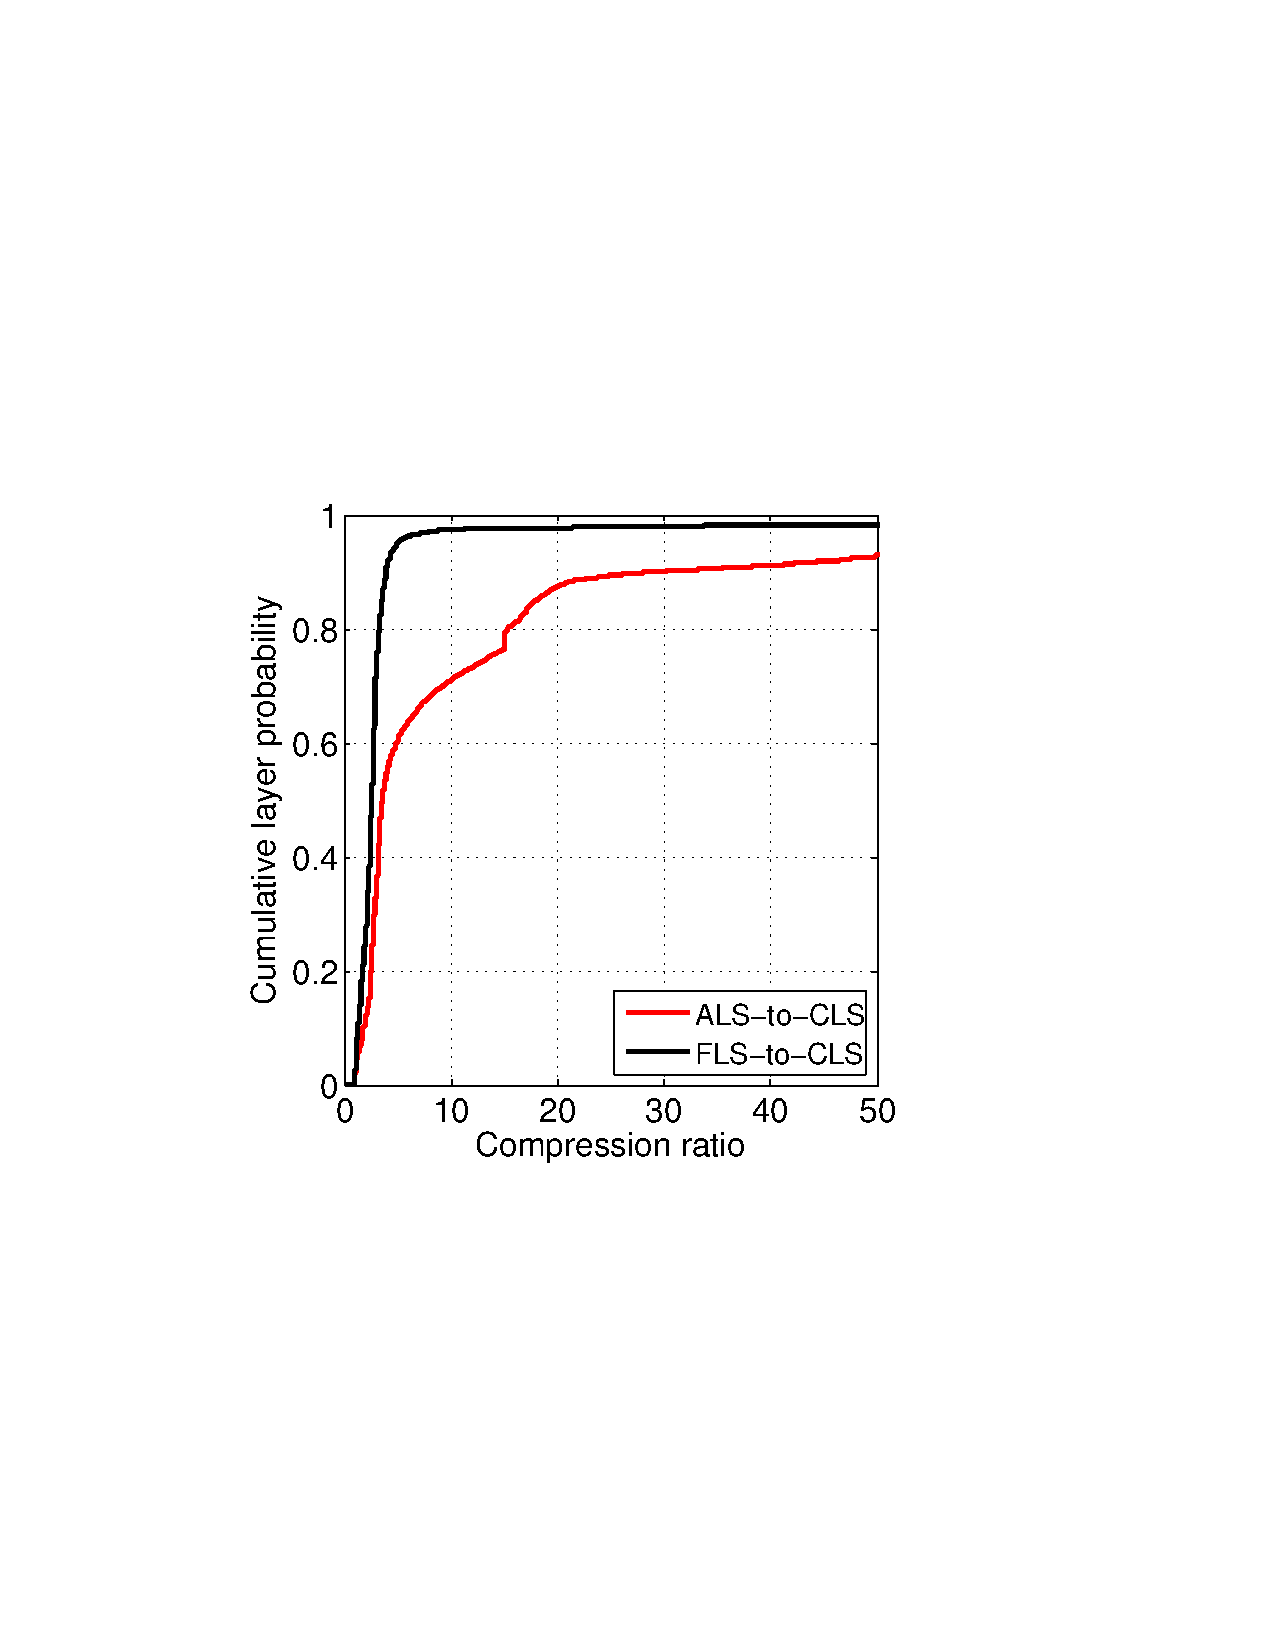
\includegraphics[width=0.23\textwidth]{graphs/cdf_compression_ratio.pdf}
	}
	\subfigure[Histogram of comp. ratios]{\label{fig_his_compression_ratio}
		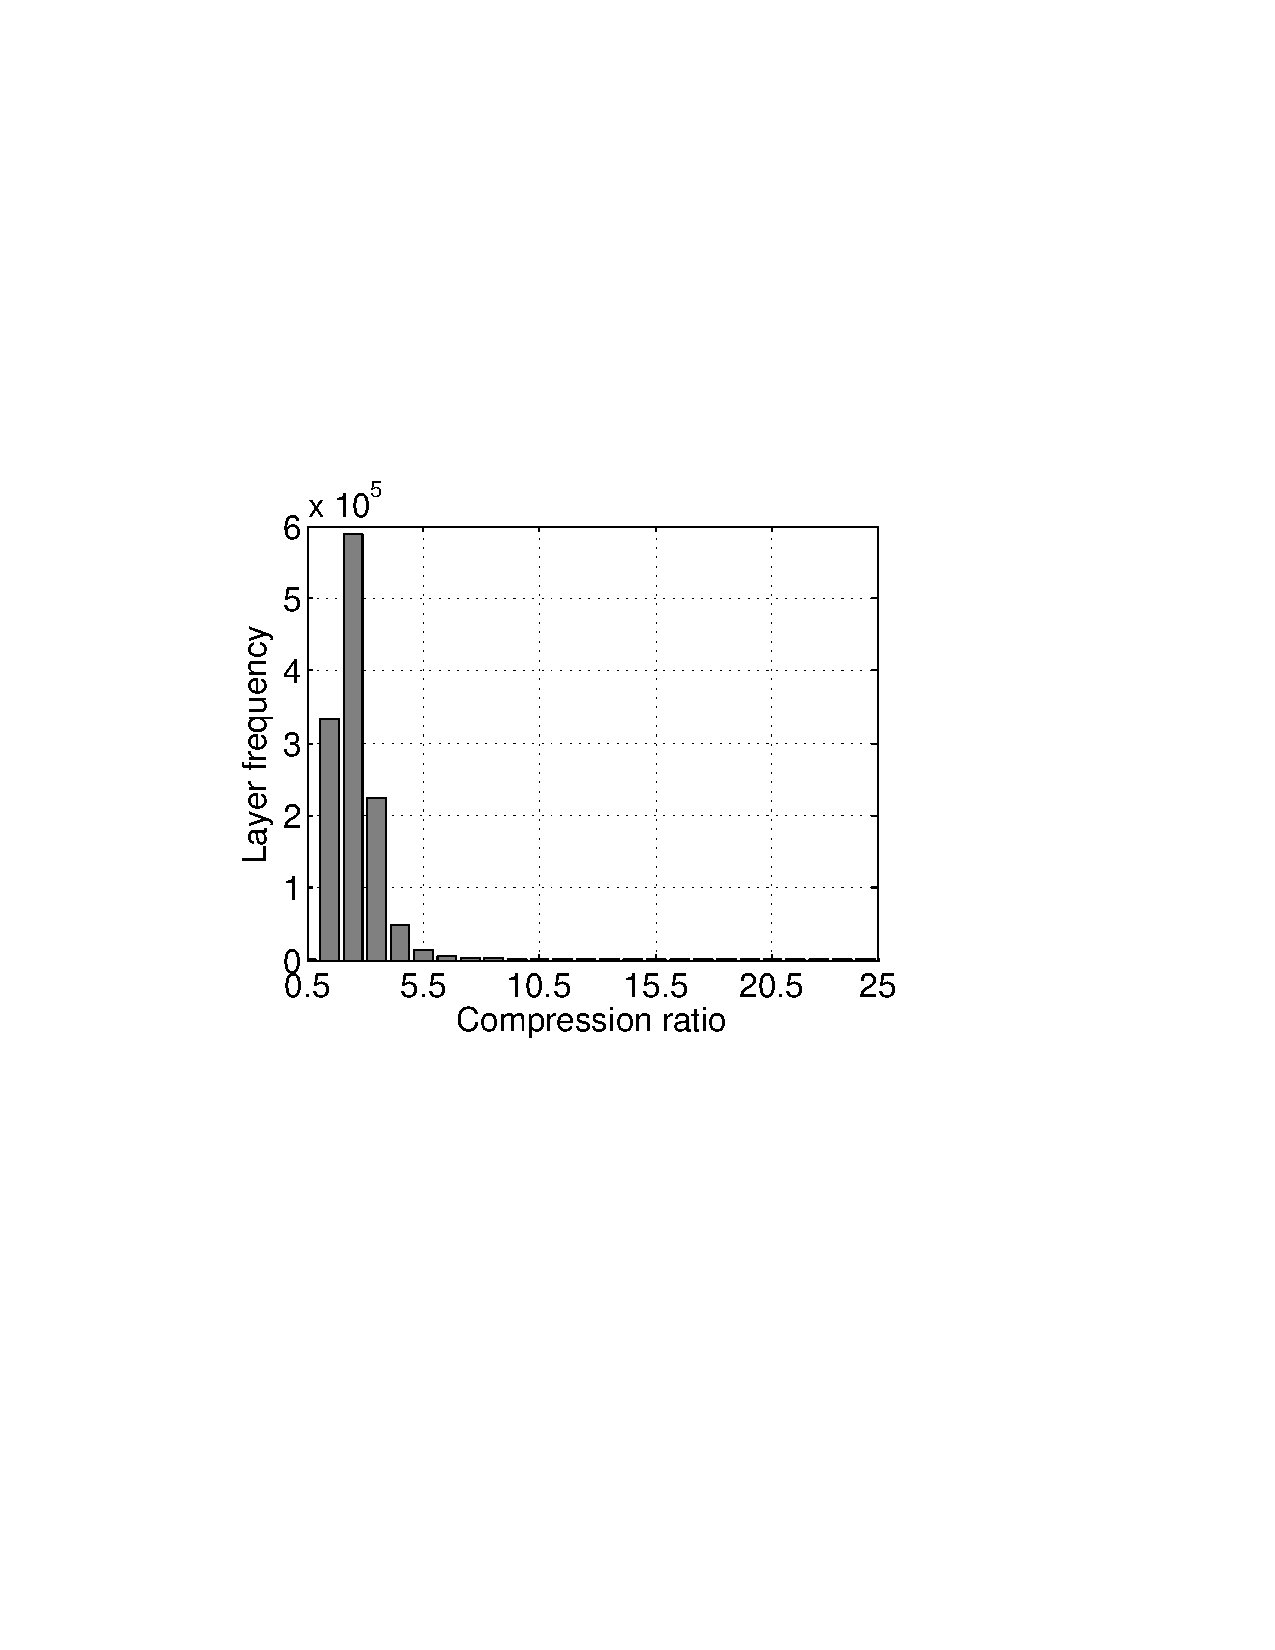
\includegraphics[width=0.223\textwidth]{graphs/his_compression_ratio.pdf}
	}
	\caption{Layer compression ratio distribution
	%\vcomment{Different colors are used in figure (a) and (b) FLS/CLS\nancomment{will address later}}
	}
	\label{fig-compression-ratio}
\end{figure}


%\paragraph{Layer compression ratios}

To further study the sizes and the impact of compression, we calculate
the FLS-to-CLS compression ratios (see Figure~\ref{fig_cdf_compression_ratio}).
%
%The ALS-to-CLS ratio is generally greater than the FLS-to-CLS ratio
%because small files in layers get larger when combined in a tar archive.
%
90\% of layers have a  CLS-to-FLS ratio less than 4 and the median
compression ratio is 2.6. The largest compression ratio is 1026.
%
%Half of the layers have a compression ratio (both ALS-to-CLS and
%FLS-to-CLS) around 3.
%
%
%The maximum FLS-to-CLS is 512,930 and maximum ALS-to-CLS is 1026.
%
Looking at the histogram (see Figure~\ref{fig_his_compression_ratio}), we see
that around 600,000 layers have a compression ratio of between 1.5 and 2.5\nancomment{it is between 2 and 3} while more than
300,000 between 0.5 and 1.5\nancomment{it is between 1 and 2}.
%
%Two peaks in the graph correspond to 587,000 layers that have the FLS-to-CLS ratio of 3
%and 331,000 layers that have the ALS-to-CLS ratio of 3.

Our size analysis reveals an interesting trade-off. Compression is computationally
expensive and is one of the major sources of latency when pulling an image from Docker Hub.
As the majority of layers is small and has low compression ratios, it can
be beneficial to store small layers uncompressed in the registry to reduce pull latencies.

%%%%%%%%%%%%%%%%%%%%%%%%%%%%%%%%%%%%%%%%%%%%%%%%%%%%%%%%%%%%%%%%%%%%%

\begin{figure}
	\centering
	\begin{minipage}{0.23\textwidth}
		\centering
		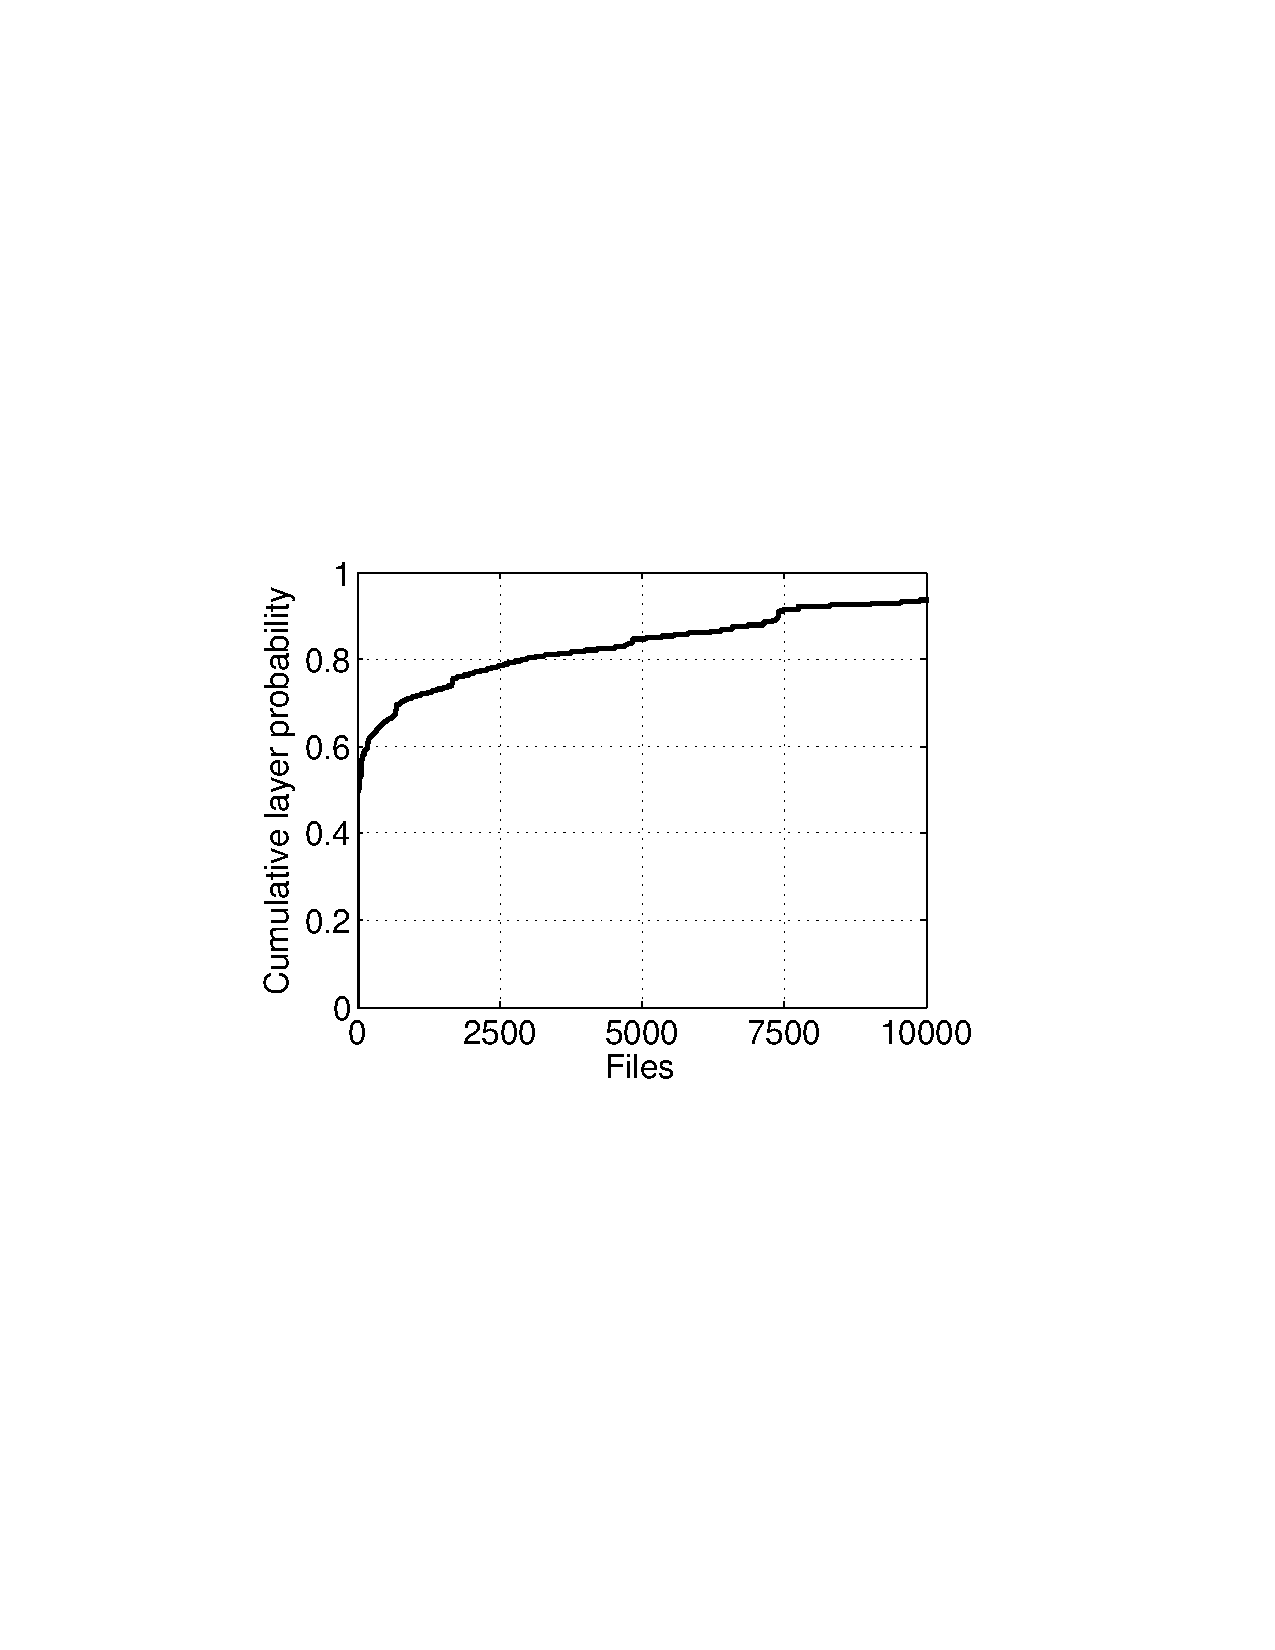
\includegraphics[width=1\textwidth]{graphs/file_cnt.pdf}
		\caption{File count distr.}
		\label{fig_file_cnt}
	\end{minipage}
	\begin{minipage}{0.23\textwidth}
		\centering
		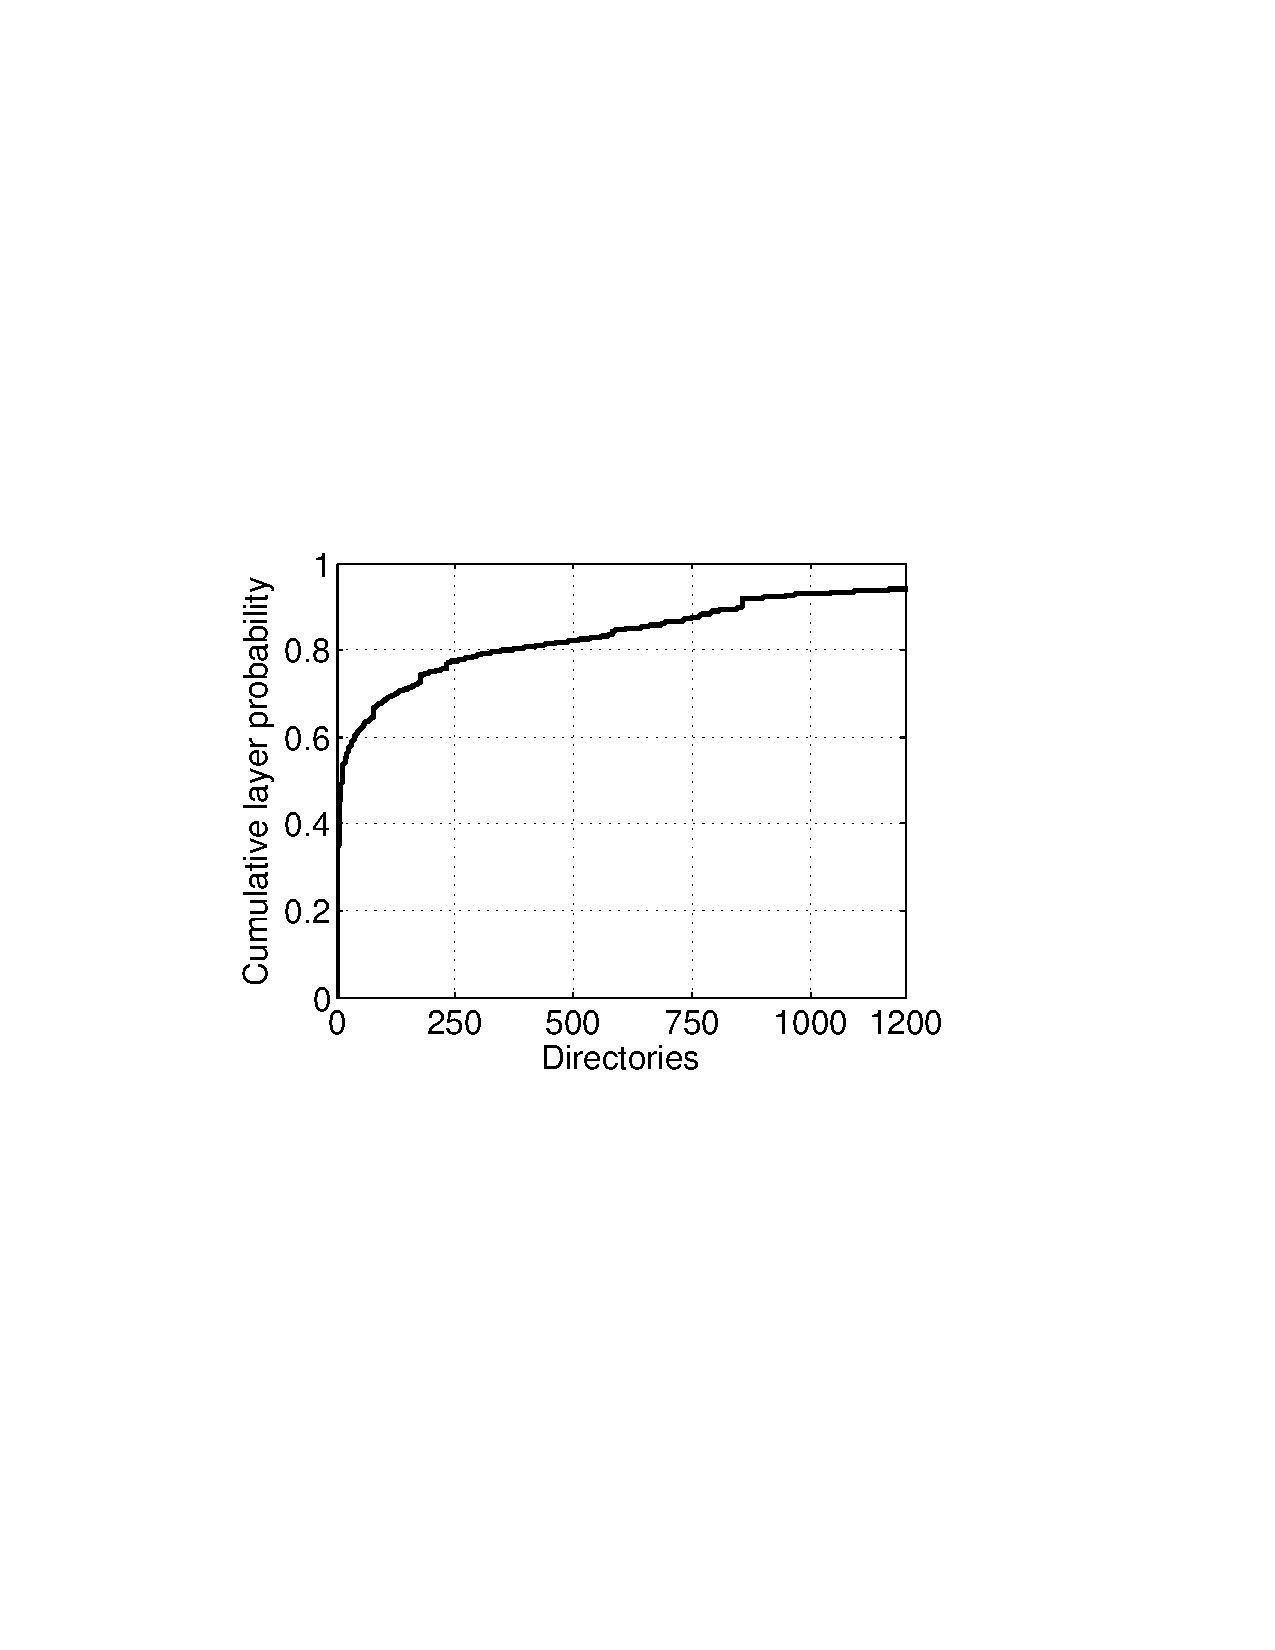
\includegraphics[width=1\textwidth]{graphs/dir_cnt.pdf}
		\caption{Dir. count distr.
		%\vcomment{Let's make thise figure subfigures.}
		}
		\label{fig_dir_cnt}
	\end{minipage}%
\end{figure}
%

\paragraph{File and directory counts}

Next, we look at file and directory metrics in layers.
Figure~\ref{fig_file_cnt} and~\ref{fig_dir_cnt} show the CDFs of file
and directory counts in all layers, respectively.
%
The results show that 90\% of layers contain less than 7,410 files while half
of the layers have less than 30 files.
%
We also found that 27\% of the layers only have a single file while 7\% even showed
no files at all. We currently do not know the exact reason for the empty layers but
plan to investigate their corresponding images in the future\nancomment{The layers are not empty since it could have directories}. On the other hand,
the largest layer contains 826,196 files which was part of a Debian image.
%
%The average is 2,200.
%
For directories, 90\% of the layers have less than 826 directories and half of the layers consist
of less than 11 directories. We again observe a wide range with a minimum of a single directory
and a maximum of 111,940. The layer with the most directories was part of
the \textit{conjurinc/developer-quiz} image.

%\paragraph{Directory depths}

%After extracting and unpacking gzip compressed layer archival files,
Besides the count, we also calculate the maximum directory depth for every layer
(see Figure~\ref{fig_layer_depth}).
%
Around 90\% of all layers have a directory depth less than 10
while for 50\%  of the layers, the directory depth is less than 4. 
%
The most frequent directory depth is 3 with 313,000 layers showing
this depth value (see Figure~\ref{fig_hist_layer_depth}.
%
%About 313,000 layers' layer directory depth is 3, which is the peak value in
%the figure.
%
%The maximum repeat count is 444 while the median is 4. The average is ~5.

This analysis shows that the majority of layers consists only of a small number
of files and does not contain deeply nested directory hierarchies. Hence, except
a few outliers, layers do not require a large amount of metadata from the storage
system.

\begin{figure}[!t]
	\centering
	\subfigure[CDF of layers by layer directory depth]{\label{fig_layer_depth}
		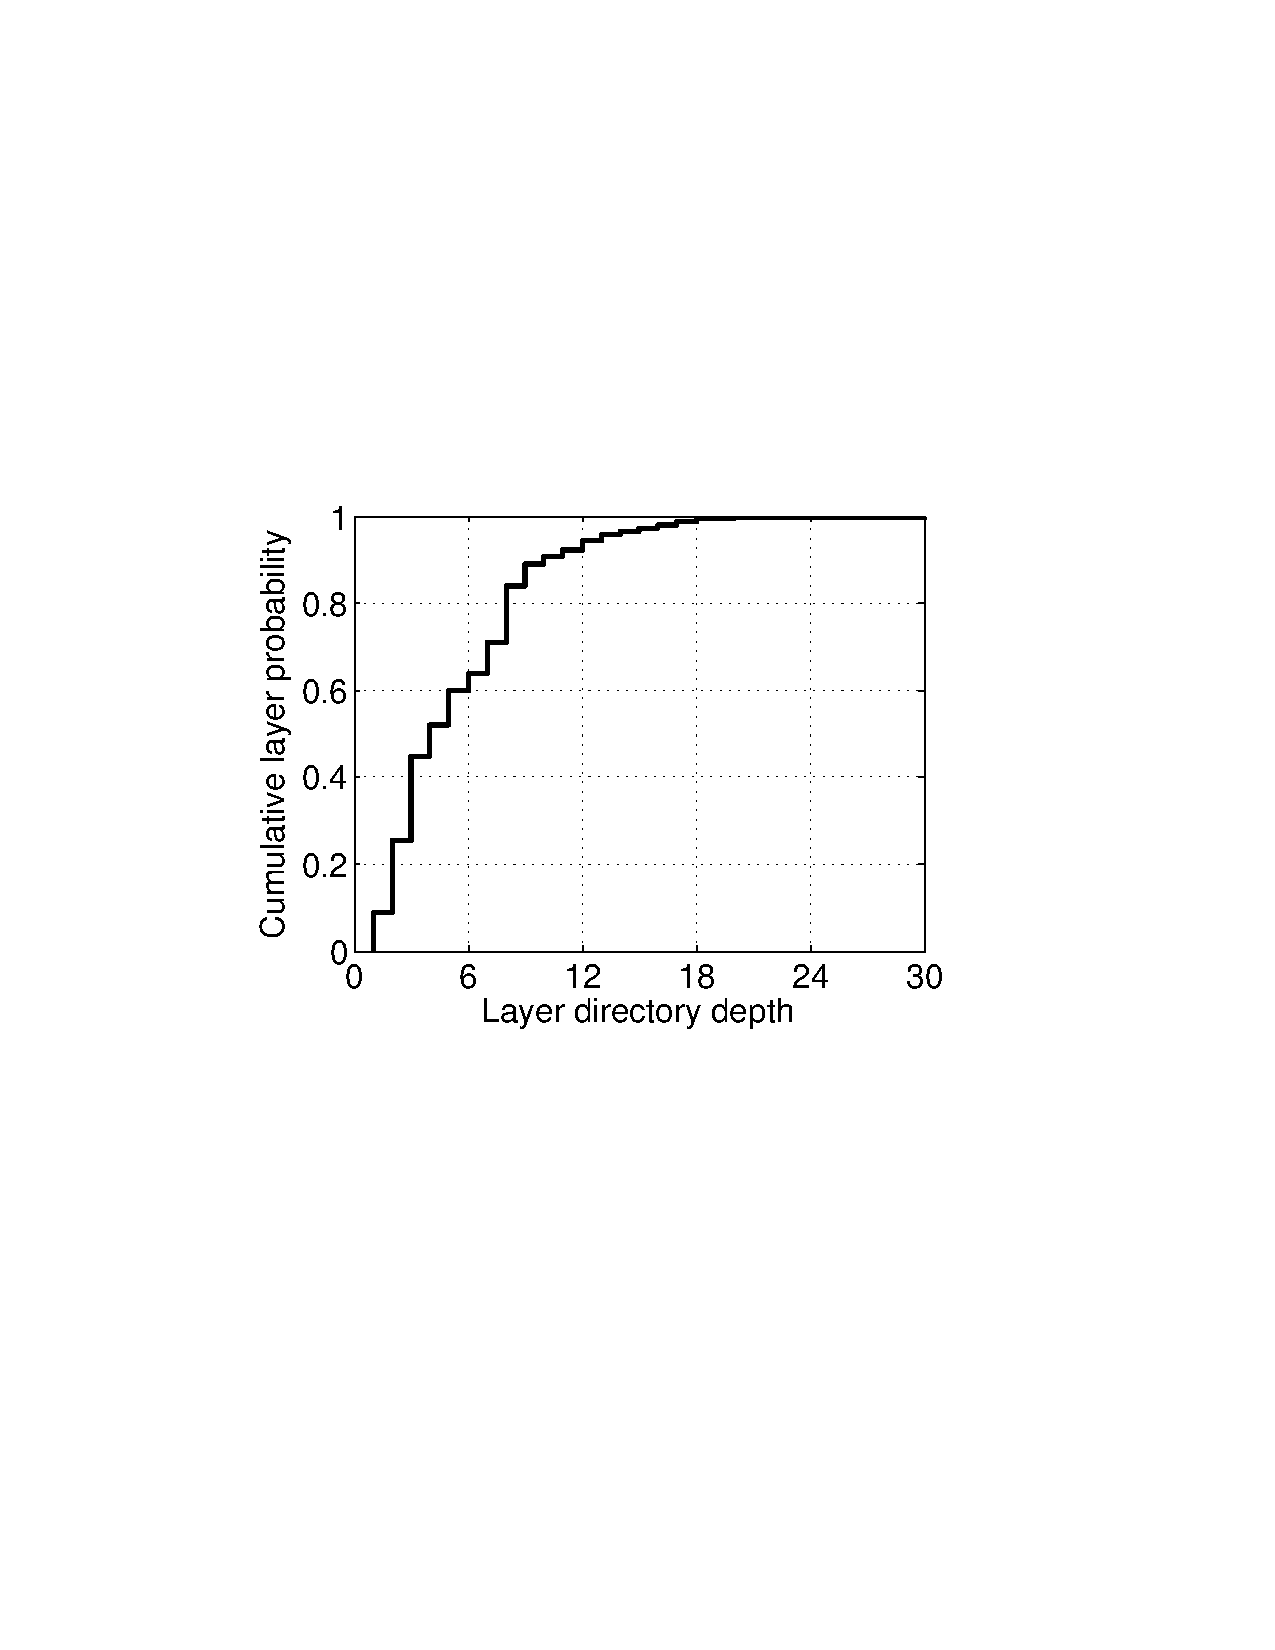
\includegraphics[width=0.23\textwidth]{graphs/layer_depth.pdf}
	}
	\subfigure[Histogram of layers by layer directory depth]{\label{fig_hist_layer_depth}
		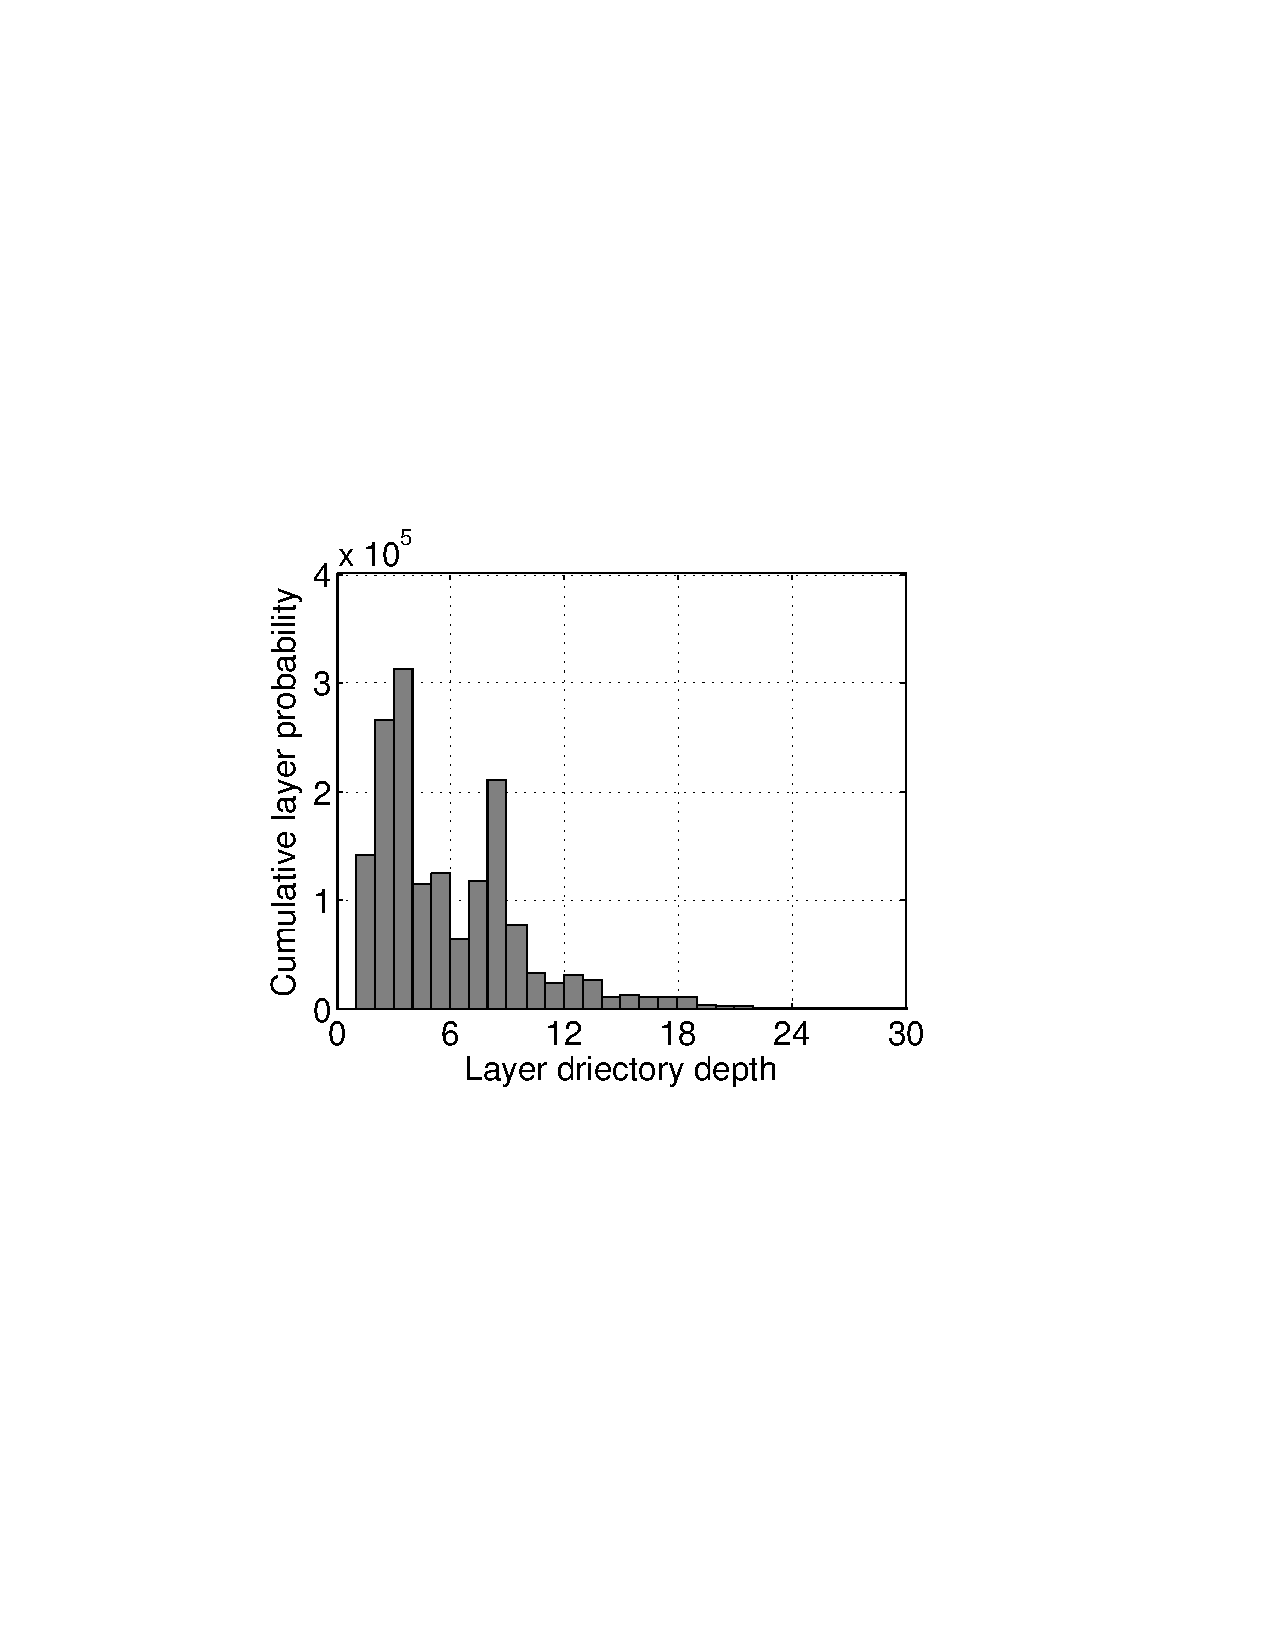
\includegraphics[width=0.22\textwidth]{graphs/hist_layer_depth.pdf}
	}
	\caption{Layer directory depth distribution}
	\label{fig-layer-dir}
\end{figure}

\subsection{Images}
\label{sec:images}

We continue analyzing images and present the following useful metric distributions: image size and compressibility, layer reference count, file and directory
counts. 

\paragraph{Image size}%{Layer and image size}

%80\% of images are less than 794 MB in uncompressed format
%80\% of images are less than 312 MB in compressed format
%
%50\% 406
%50\% 157

%\nancomment{add pdf if can}
%\acomment{Where is layers analysis when you say similarly? I wrote above
%para.. see for consistency.}
%Conatiner image size determines the runtime of container if it is not already
%cached locally. 
Similar to layers, we measured compressed and uncompressed image size. 
Figure~\ref{fig:image-size-cdf} show the image size distributions. 
%and a finer resolution only covering images smaller than 1.5 GB.
%\acomment{Could not locate the figures you are talking about. I see two figures
%layers size and image size.}
We find that 80\% of the images have an uncompressed size less than
794 MB and compressed size of 312 MB.
%while compressed images are less than 0.48 GB. 
In the median, this decreases to 406 MB and 157 MB, respectively. The largest
uncompressed image is 498 GB which is a Ubuntu-based image.  

\emph{Figure~\ref{fig:image-size-cdf} shows that the majority of uncompressed images in
Docker Hub are small which aligns with the Docker philosophy to package
software and distribute software in containers but include only its necessary
dependencies.}

\paragraph{Compression ratio}
%\begin{figure}
%	\centering
%	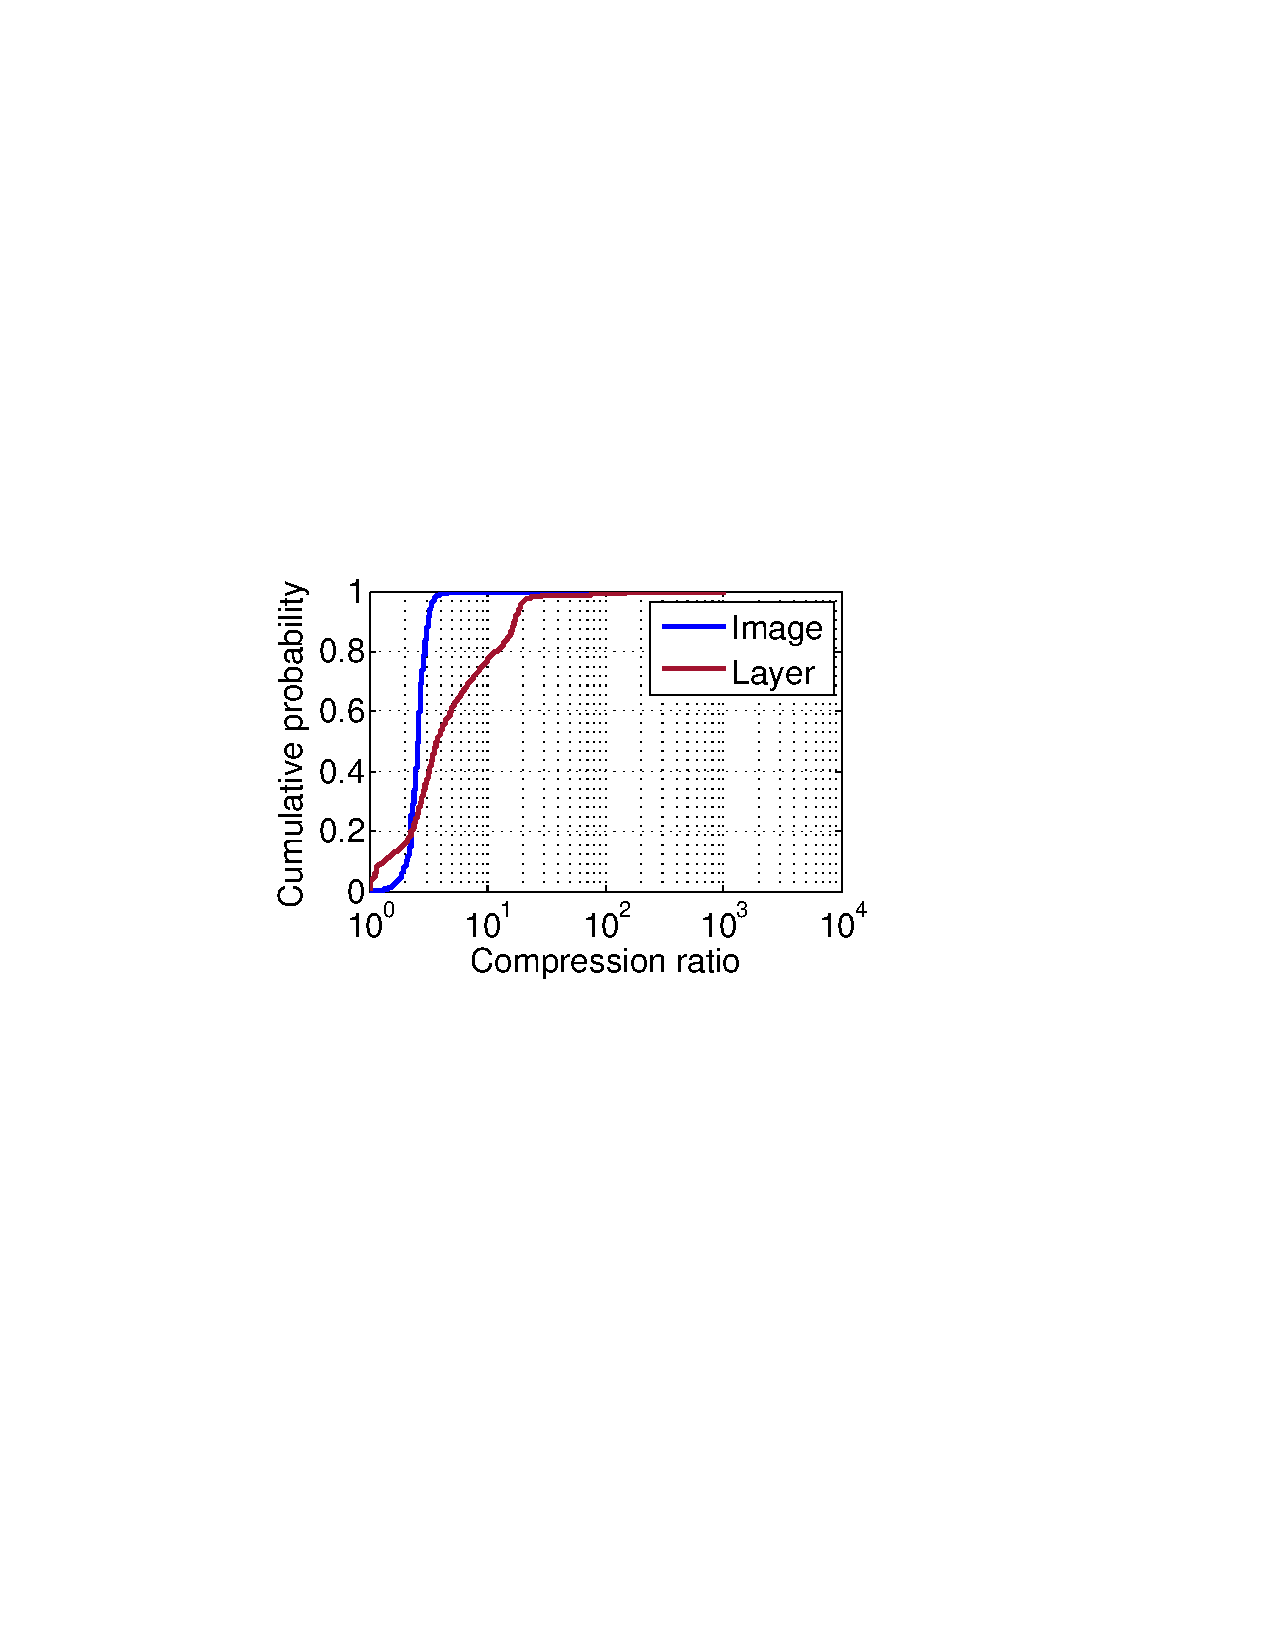
\includegraphics[width=0.4\textwidth]{graphs/compress-ratio-cdf.pdf}
%	\caption{CDF of compression ratio.
%	}
%	\label{fig:compress-ratio}
%\end{figure}

%\begin{figure}[!t]
%	\centering
%	\subfigure[Image compression ratio]{\label{fig_hist_image}
%		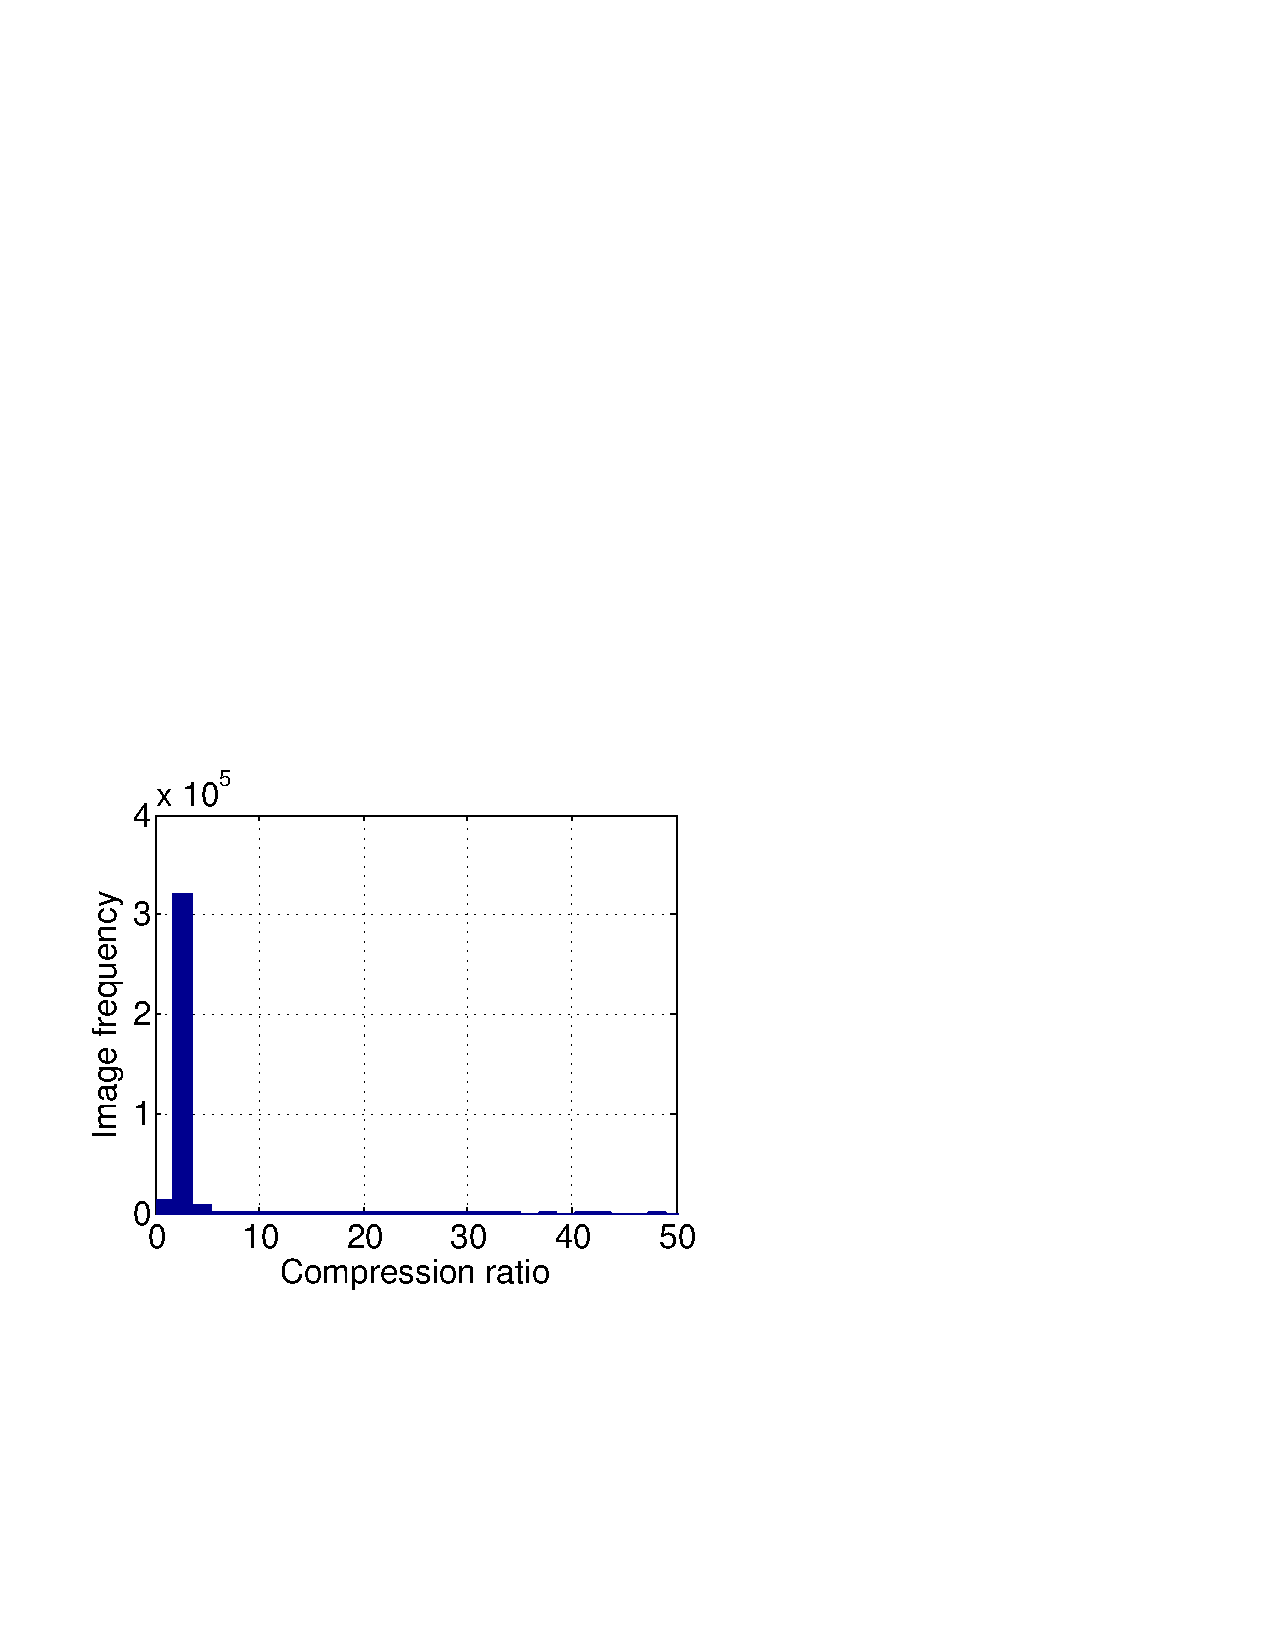
\includegraphics[width=0.215\textwidth]{graphs/image-compress-ratio-pdf.pdf}%
%	}
%	\subfigure[Layer compression ratio]{\label{fig_hist_layer}
%		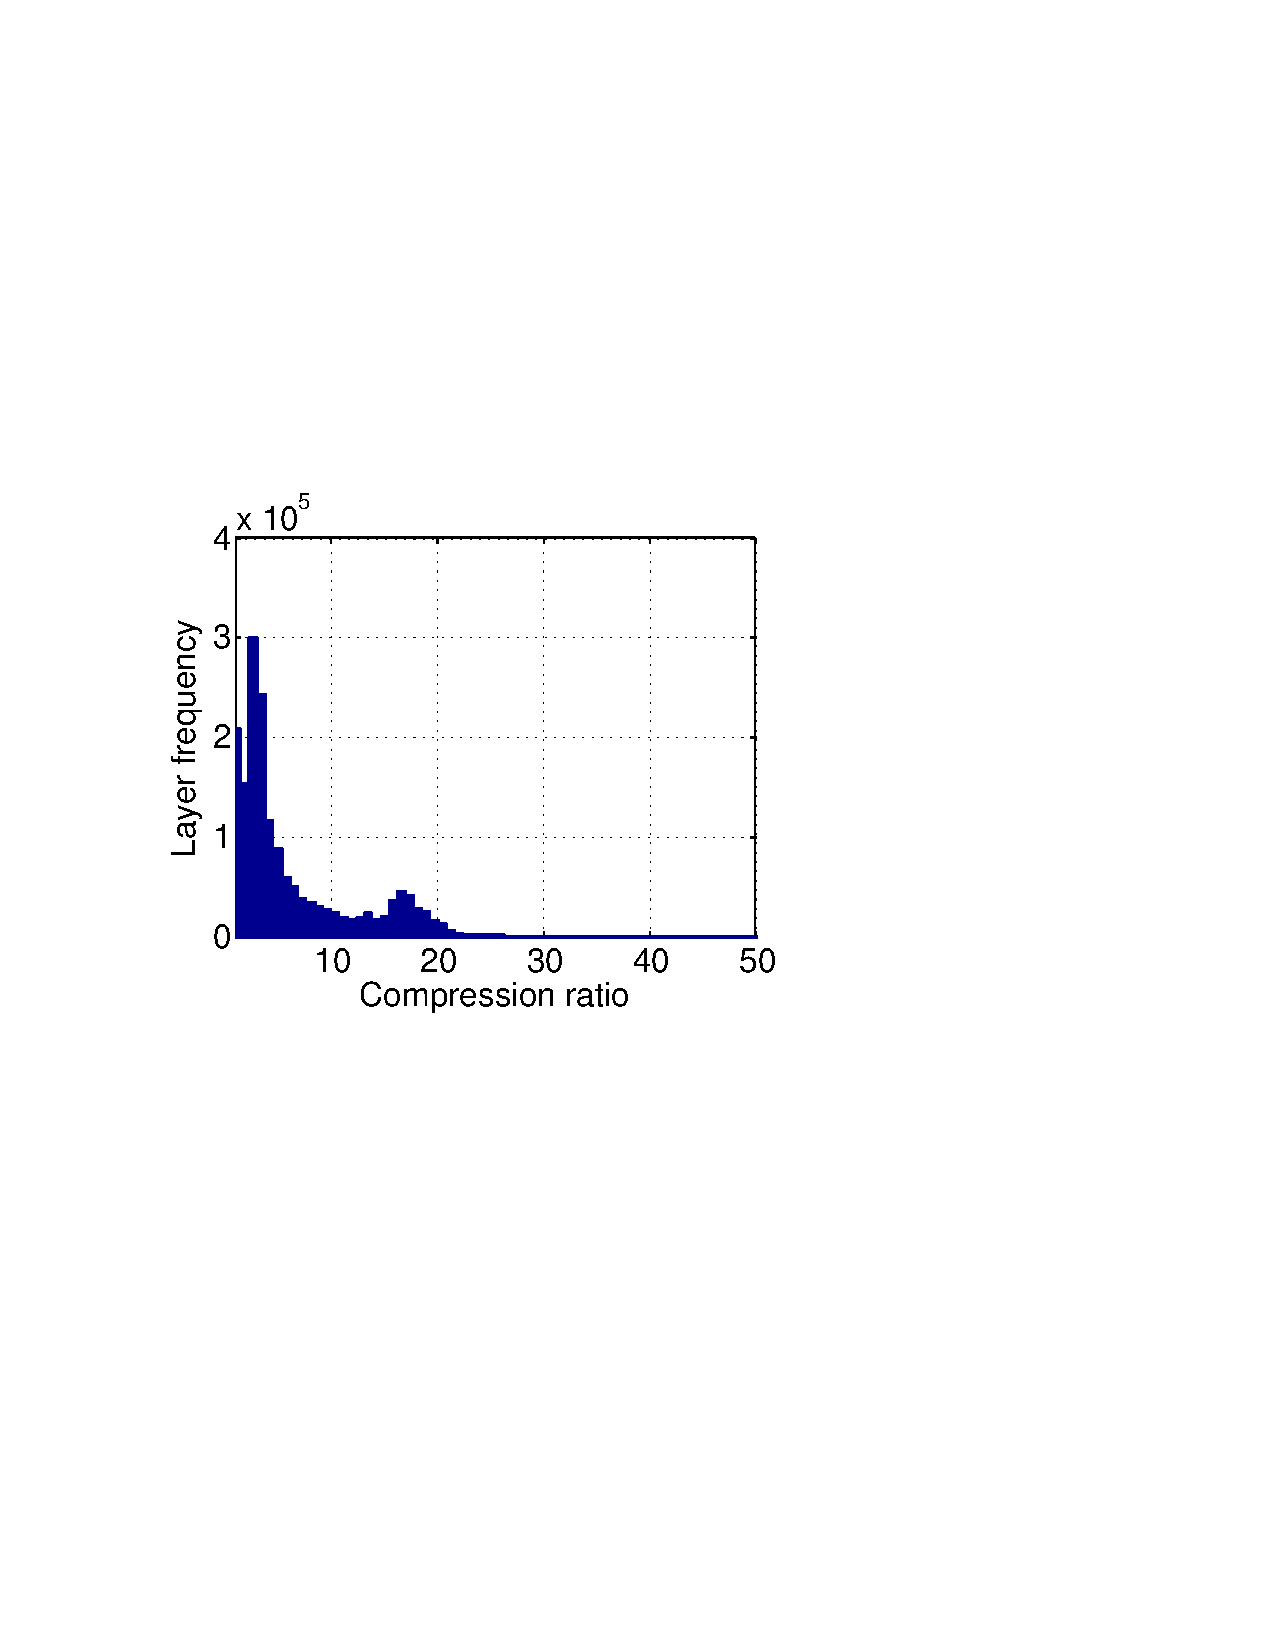
\includegraphics[width=0.22\textwidth]{graphs/layer-compress-ratio-pdf.pdf}
%	}
%	\caption{Histogram of image and layer compression ratio.}
%	\label{fig:reference-cnt}
%\end{figure}

%Figure~\ref{fig:compress-ratio} shows the compression ratio of the container
%images.    %\nancomment{there is redundancy and avg compression ratio}}

To further study the sizes and the impact of compression, we calculate the
compression ratios for images (see Figure~\ref{fig:compress-ratio}).
80\% of images have compression ratio less than 2.9 while the median is 2.6. 
\textit{We see that majority of images have a compression ratio within 2-3.}
Compare with compression ratio for layers, we see that images have a much smaller
compression ratio. 
\textit{This means that images contains both layers with high compression ratio and low compression ratio.}
%, which means images contains different layers and high . 

%\acomment{Found following para in directory count subsection..}
%
%The ALS-to-CLS ratio is generally greater than the FLS-to-CLS ratio because
%small files in layers get larger when combined in a tar archive.
%
%90\% of layers have a  compression ratio less than 4 and the median compression
%ratio is 2.6. The largest compression ratio is 1026.
%%
%Half of the layers have a compression ratio around 3.
%
%
%The maximum FLS-to-CLS is 512,930 and maximum ALS-to-CLS is 1026.
%
%Looking at the histogram (see Figure~\ref{}), we see
%that around 600,000 layers have a compression ratio of between 2 and 3 while
%more than 300,000 between 1 and 2.
%
%Two peaks in the graph correspond to 587,000 layers that have the FLS-to-CLS
%ratio of 3 and 331,000 layers that have the ALS-to-CLS ratio of 3.

\paragraph{Layer count per image}
%\nancomment{more layer more matedata? overhead for union fs}

\begin{figure}[!t]
	\centering
	\subfigure[CDF of layer count]{\label{fig:layer_count}
		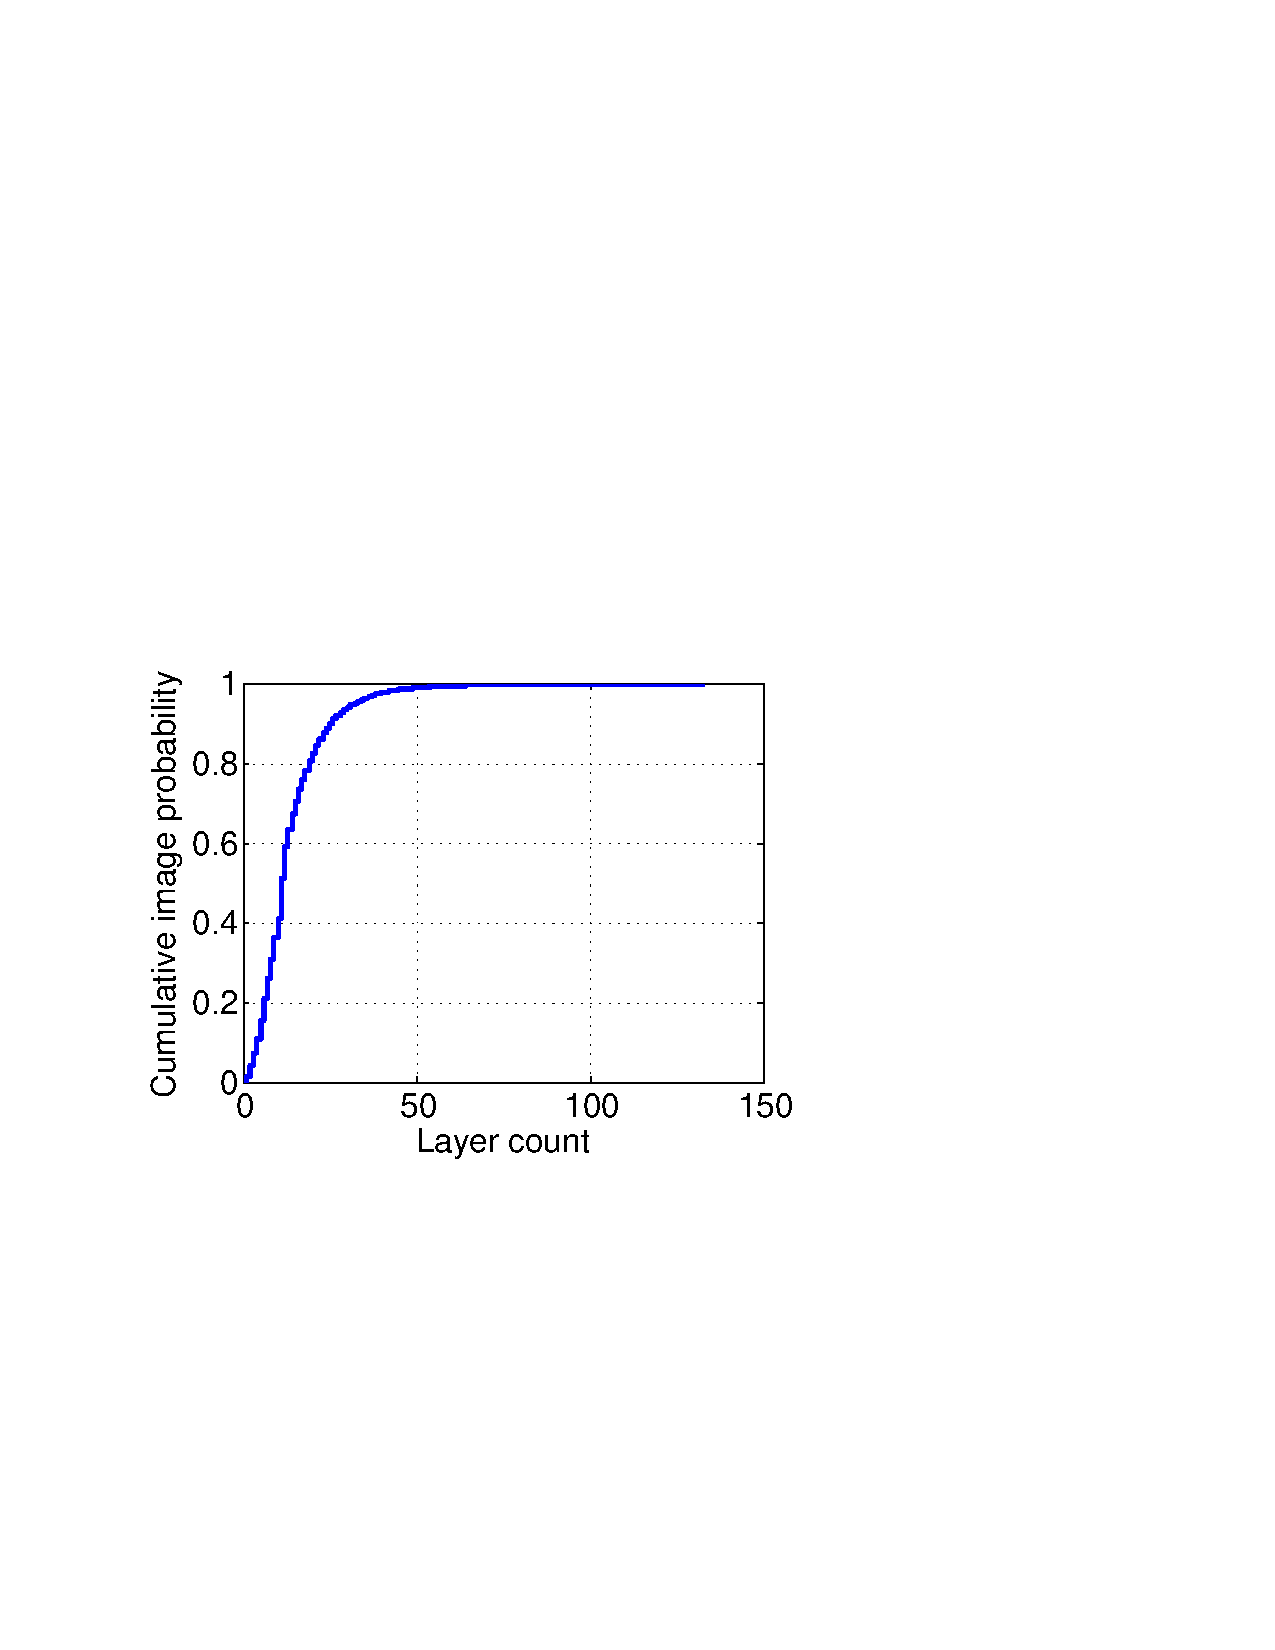
\includegraphics[width=0.215\textwidth]{graphs/image-layer-cnt}%
	}
	\subfigure[Histogram of layer count]{\label{fig:hist_layer_count}
		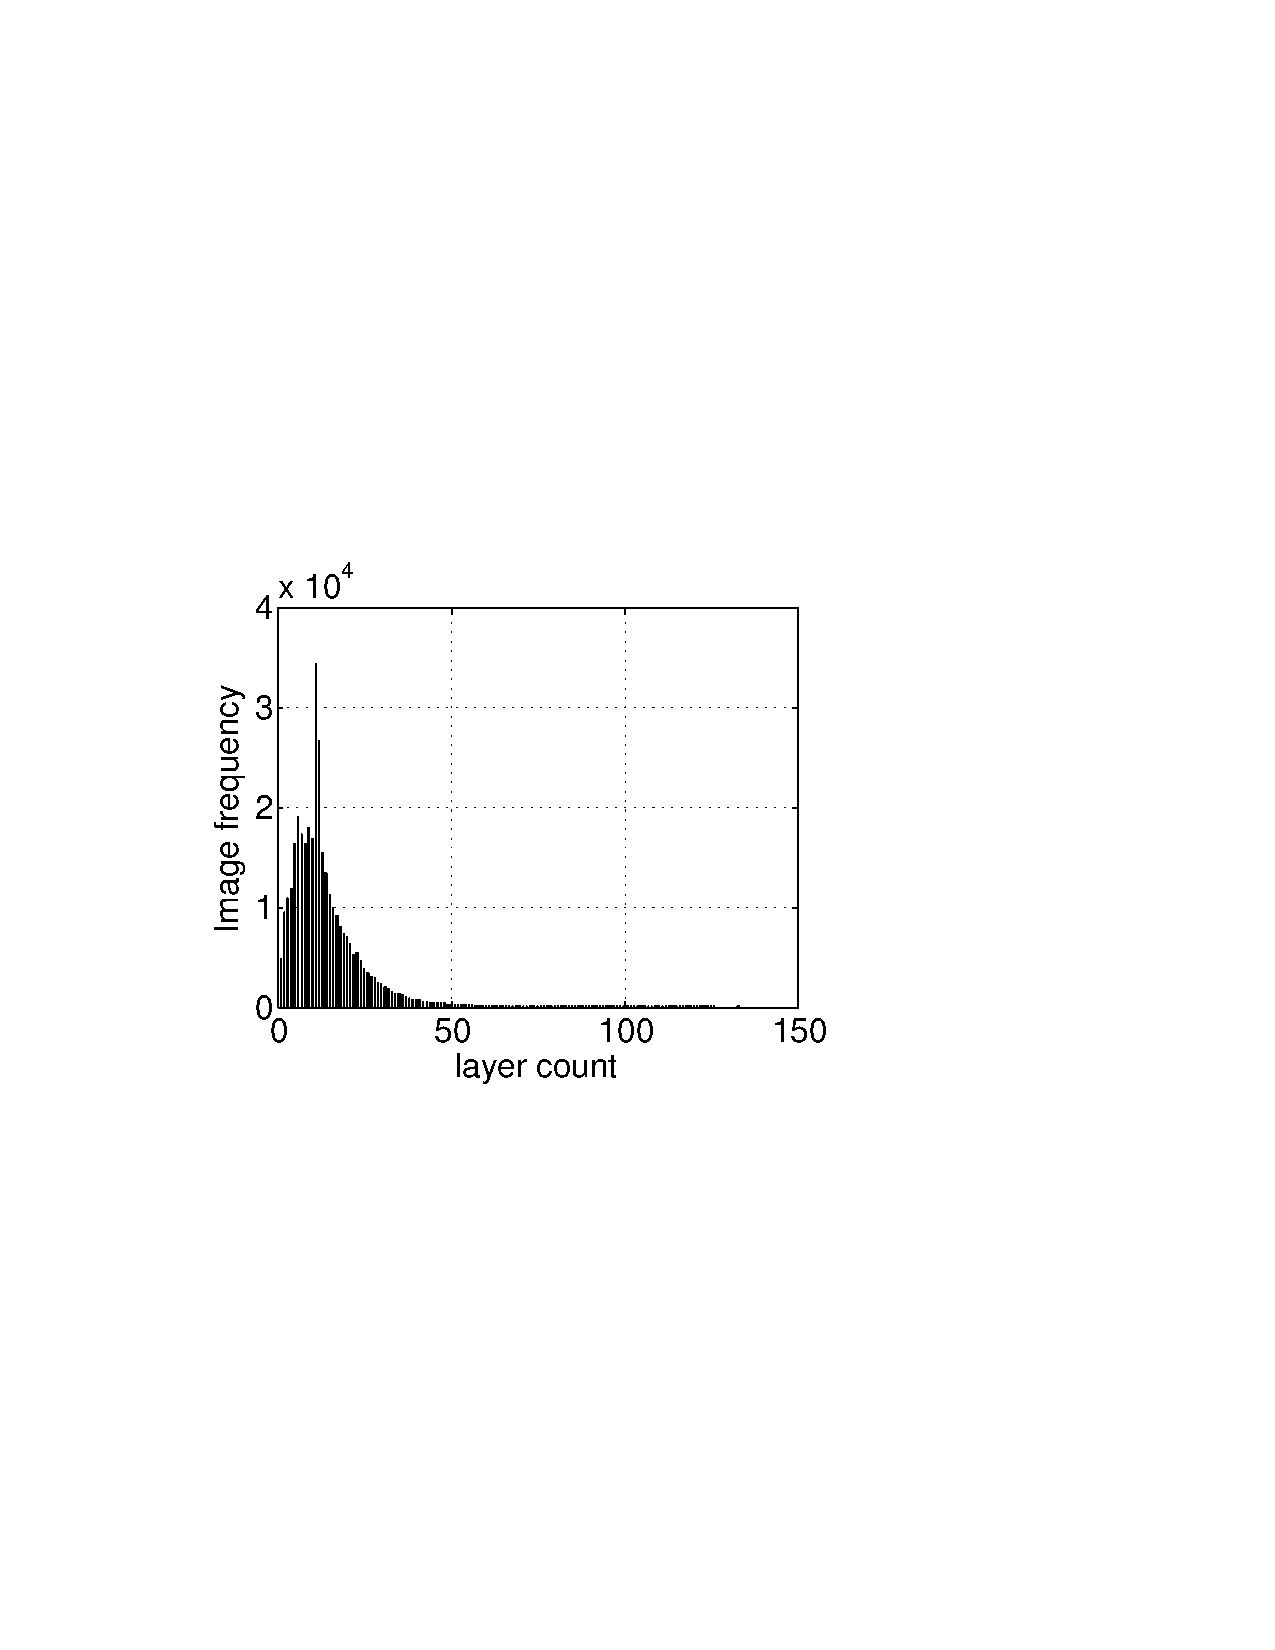
\includegraphics[width=0.21\textwidth]{graphs/image-layer-cnt-pdf.pdf}
	}
	\caption{CDF and histogram of Layer count per image.}
	\label{fig:image-size}
\end{figure}

As discussed in~\ref{sec:layers}, images consist of a set of layers.
It is important to understand the layer count of the images as previous
work found that the number of layers can impact the performance of
I/O operations~\cite{slacker}. Therefore, we count the number of layers
per image and plot the CDF (see Figure~\ref{fig:layer_count})
and layer count frequencies (see Figure~\ref{fig:hist_layer_count})for all
Docker Hub images.

The results show that 90\% of the images have less than 26 layers while
half of the images have less than 10 layers. 11 layers is also the most
frequent layer value with 34,420 images consisting of exactly 11 layers.
The maximum layer count is 120 in the \textit{cfgarden/120-layer-image}.
We also find that there are 4,792 images which only consist of a single layer.

\emph{As a rule of thumb, less number of layers is better for the union file
	system as it then needs to handle less metadata. However, as a tradeoff,
	reducing the number of layers significantly effects the data sharing among images.
	%As a result, we see less number of layers shared among different images.
	For an example, if a image consists of only single layer its data can not be shared
	with other images.}
%\begin{figure}[!t]
	\centering
	\subfigure[CDF of layer reference count]{\label{fig_repeate_layer}
		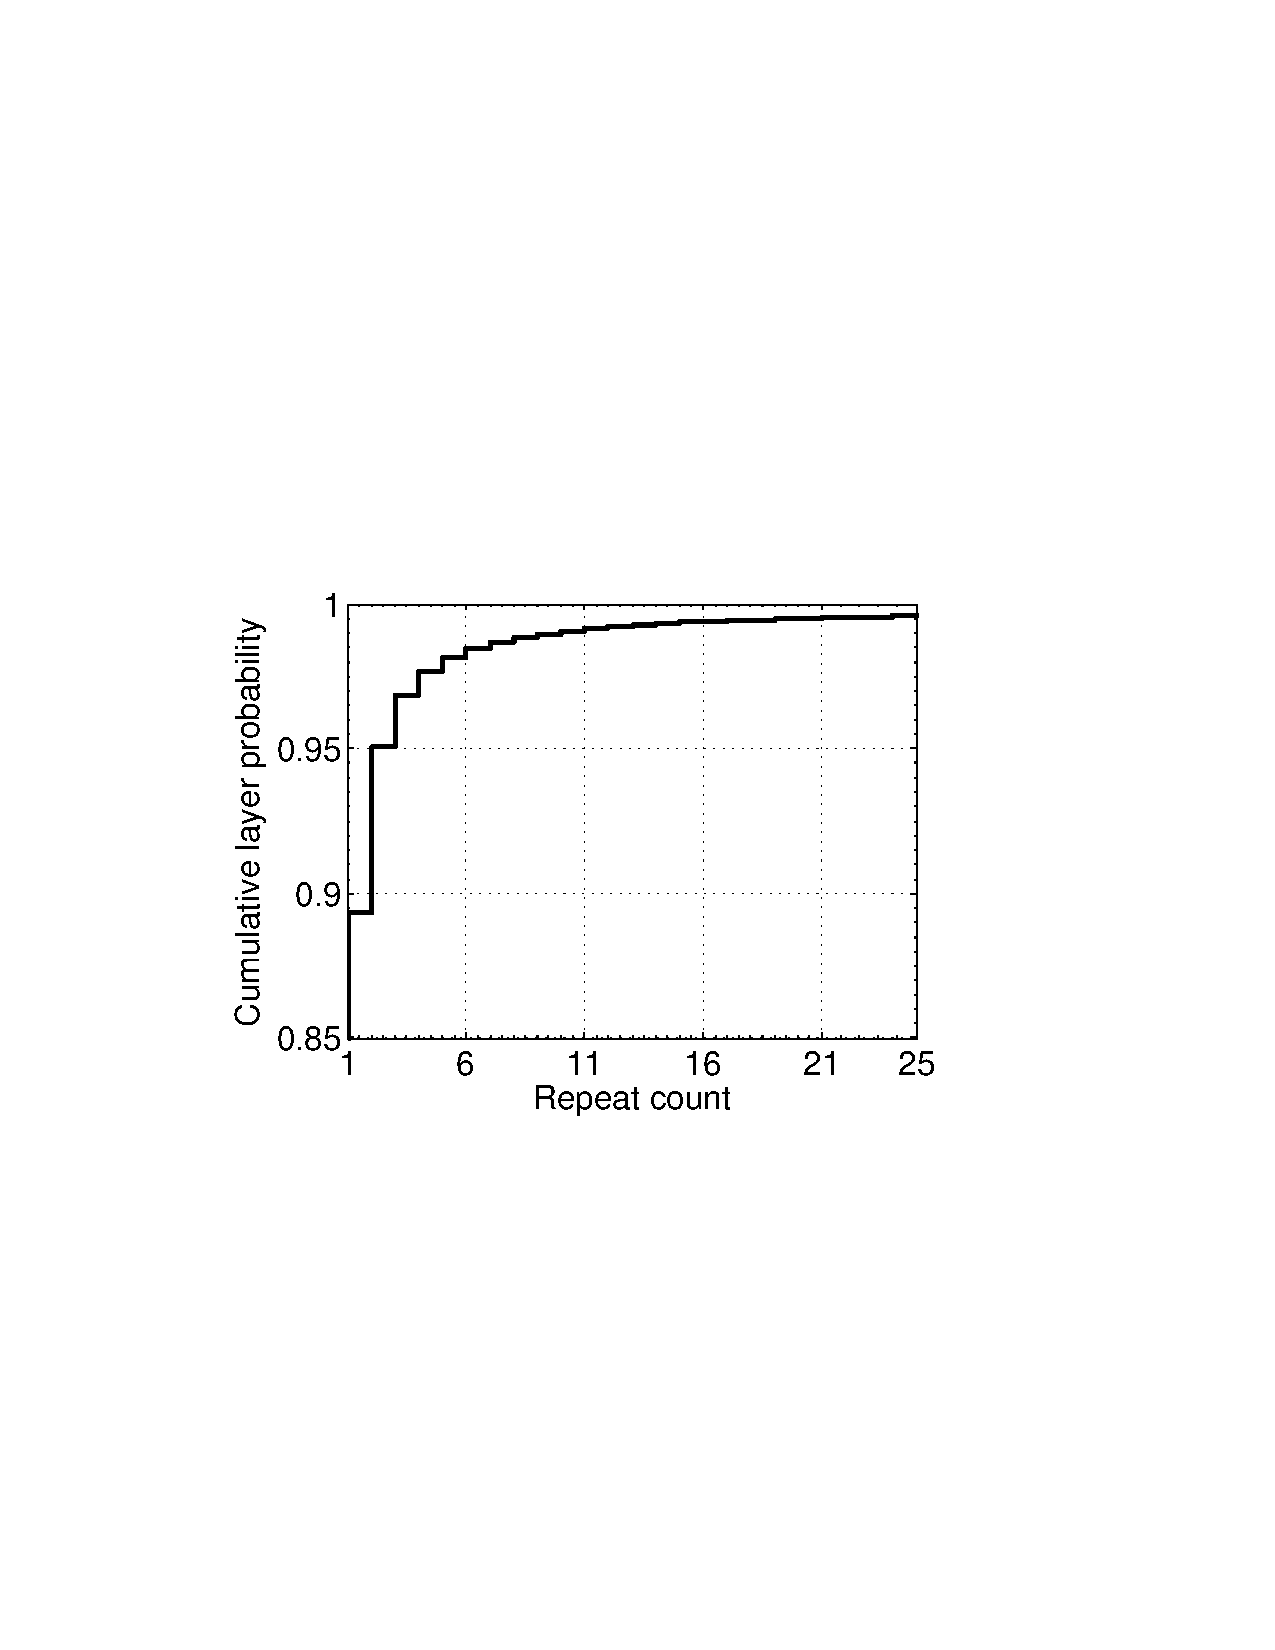
\includegraphics[width=0.23\textwidth]{graphs/repeate_layer.pdf}
	}
	\subfigure[Histogram of layer reference count]{\label{fig_hist_repeate_layer}
		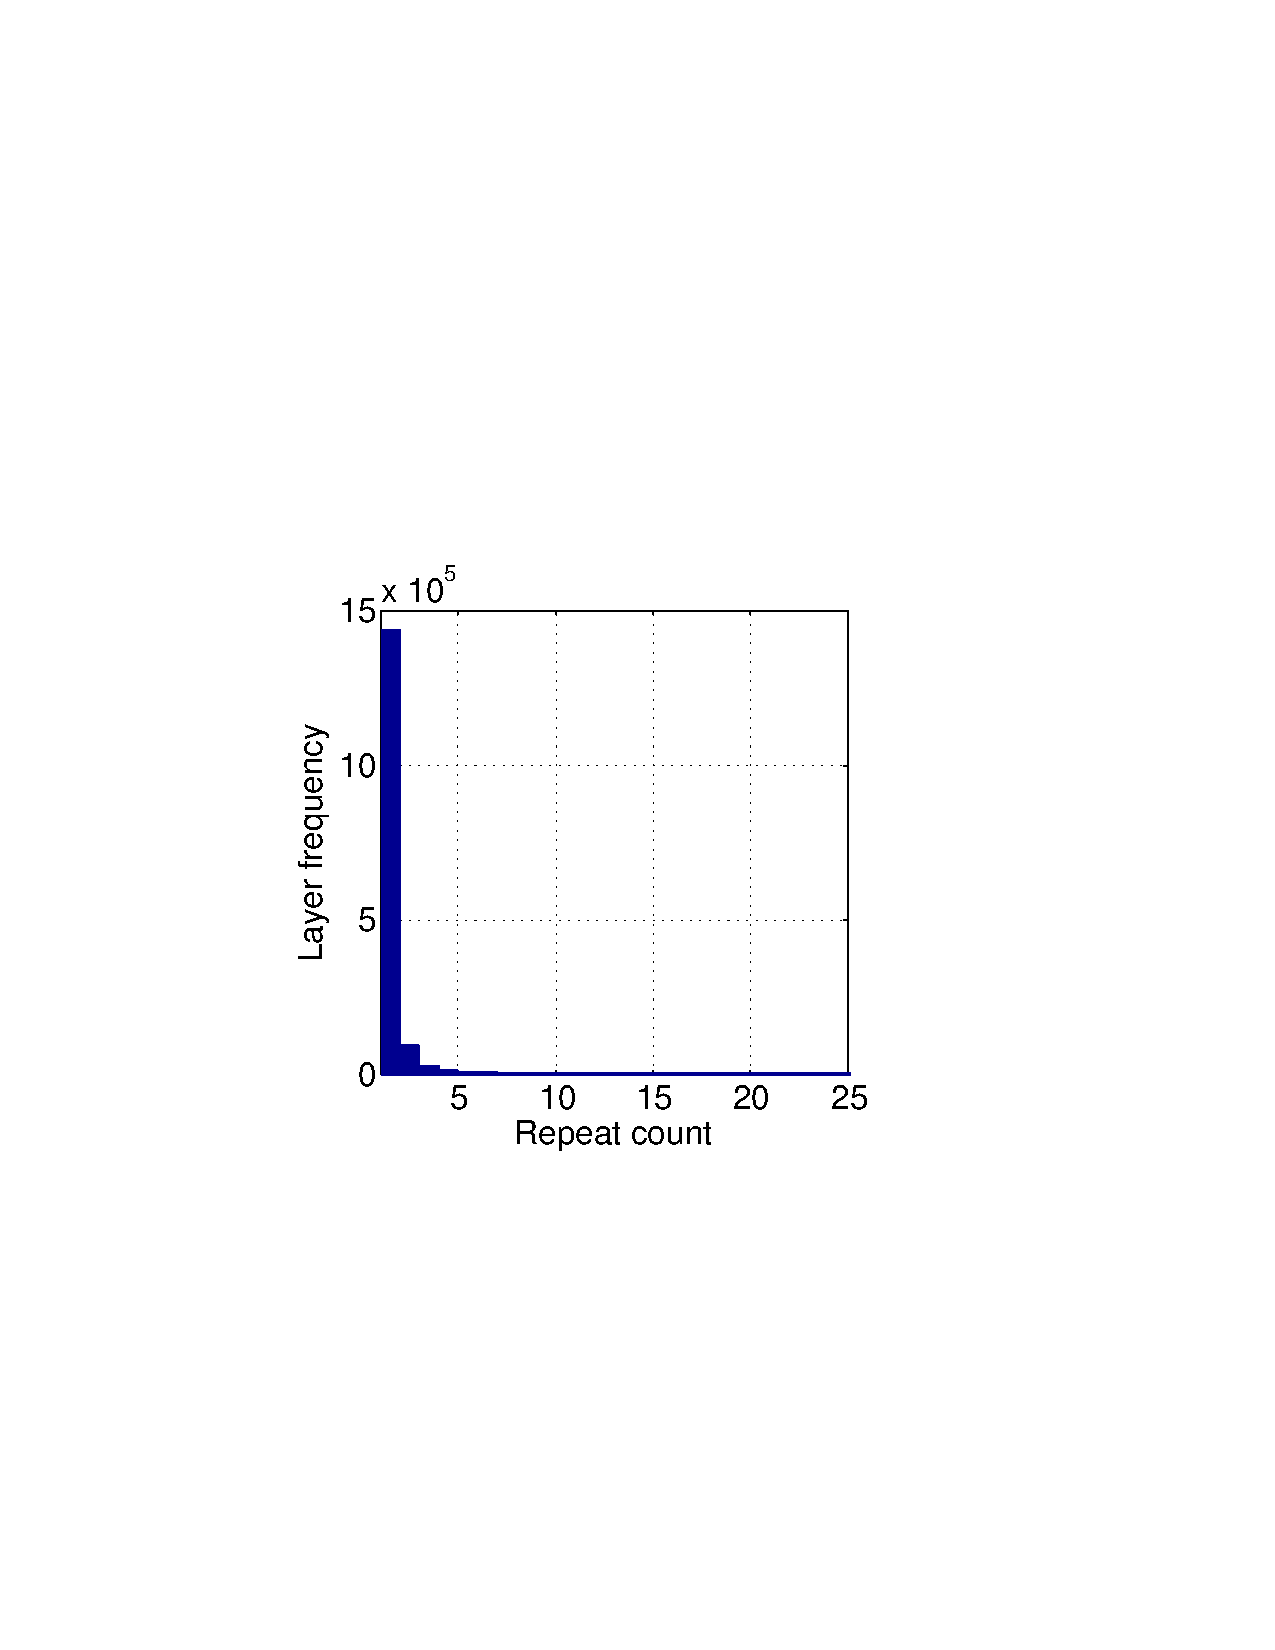
\includegraphics[width=0.223\textwidth]{graphs/hist_repeate_layer.pdf}
	}
	\caption{Layer reference counts across all images}
	\label{fig-repeat-layer-cnt}
\end{figure}

%\paragraph{Repeat layer count distribution}
\paragraph{Layer reference count}
%\nancomment{should create more shared layers to remove duplicates}

\begin{figure}
	\centering
	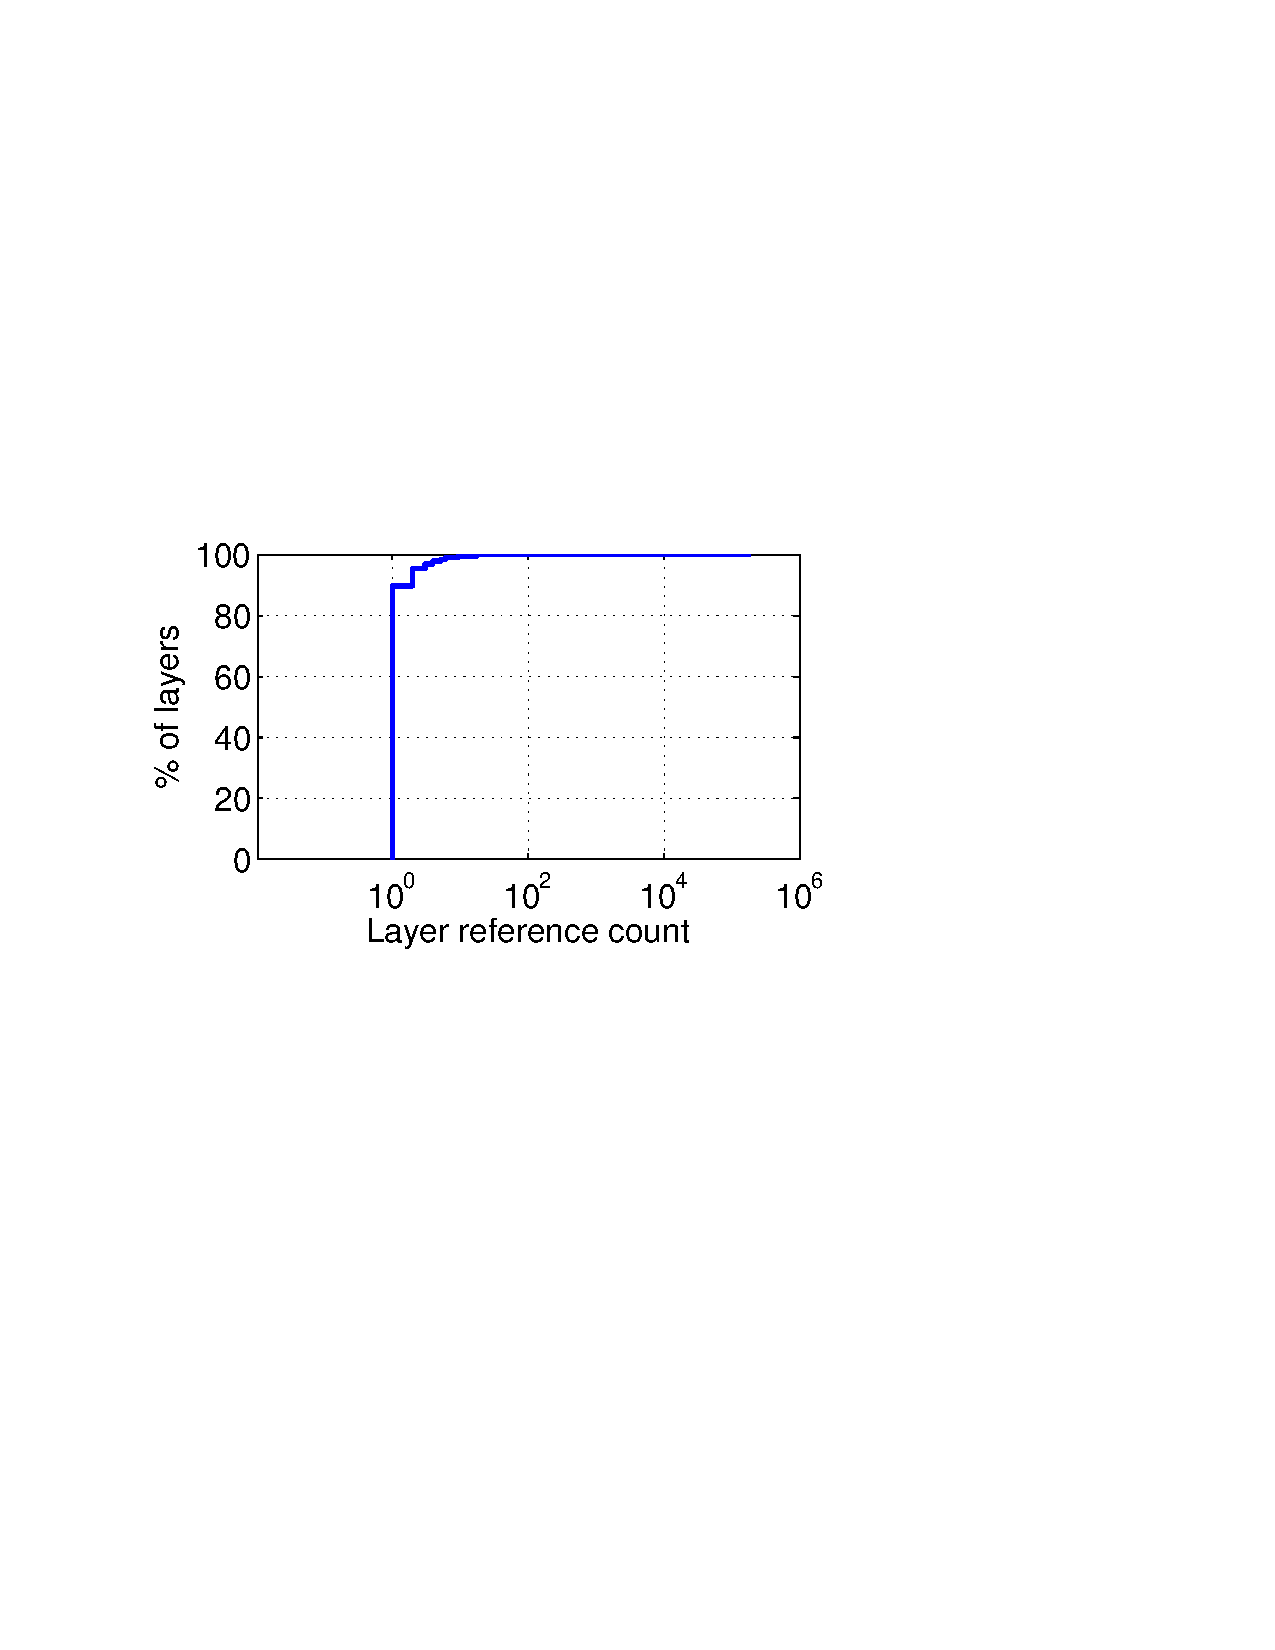
\includegraphics[width=0.21\textwidth]{graphs/shared-cnt-cdf.pdf}
	\caption{CDF of layer reference count.
	}
	\label{fig:ref_count}
\end{figure}

An interesting question is what is the sharing rate of layers across images.
We analyze all image manifests and count for each layer, how many times it is
referenced by an image. Figure~\ref{fig:ref_count} shows that around 90\% of
layers are only reference by a single image while 95\% are reference by not
more than 2 images. Similarly, 99\% of layers are shared among less than 25
images. 
%Figure~\ref{} shows the absolute values, revealing that
%almost 1.5 million images are only referenced once.  \acomment{Figure is
%	missing} While there is again a large spectrum of reference counts, the maximum
%is 33,428, the vast majority of layers is not shared. 
This hints that the
layer-based approach to improve storage efficiency is barely utilized and there
is room for improvement in how to construct more sharable layers.

\emph{These findings reveal that layer level CAS has not been very successful
	and most of the layers that exists in Docker Hub are not shared among images.
	Hence, there is a dire need of a better redundancy management.}

%89\% of 1
%95.1\% 2

\paragraph{Directory count and File count}

Next, we look at the directory (Figure~\ref{fig:dir-cnt-cdf}) and file count
(Figure~\ref{fig:file-cnt-cdf}) in images to determine if deploying images requires
handling of large amounts of metadata. 
Looking at directories, we see that 50\% of images have less than 3,326 directories and 90\% of images have less than
9,692 directories. %70\% of images have more than 2,500 directories. 
For
files, 50\% of images have less than 27,194 files and 90\% of images have less than 74,266 files.

This is consistent with our analysis of layer-based file and directory counts
and the number of layers per image. Again, \textit{we conclude that most images do not
require an extensive amount of metadata when being deployed as file and
directory counts are low except for few outliers.}

%This is consistent with our analysis of layer-based file and directory counts
%and the number of layers per image. Again, we conclude that most images do not
%require an extensive amount of metadata when being deployed as file and
%directory counts are low except for few outliers.

%\begin{figure}[!t]
	\centering
	\subfigure[CDF of compression ratio]{\label{fig_cdf_compression_ratio}
		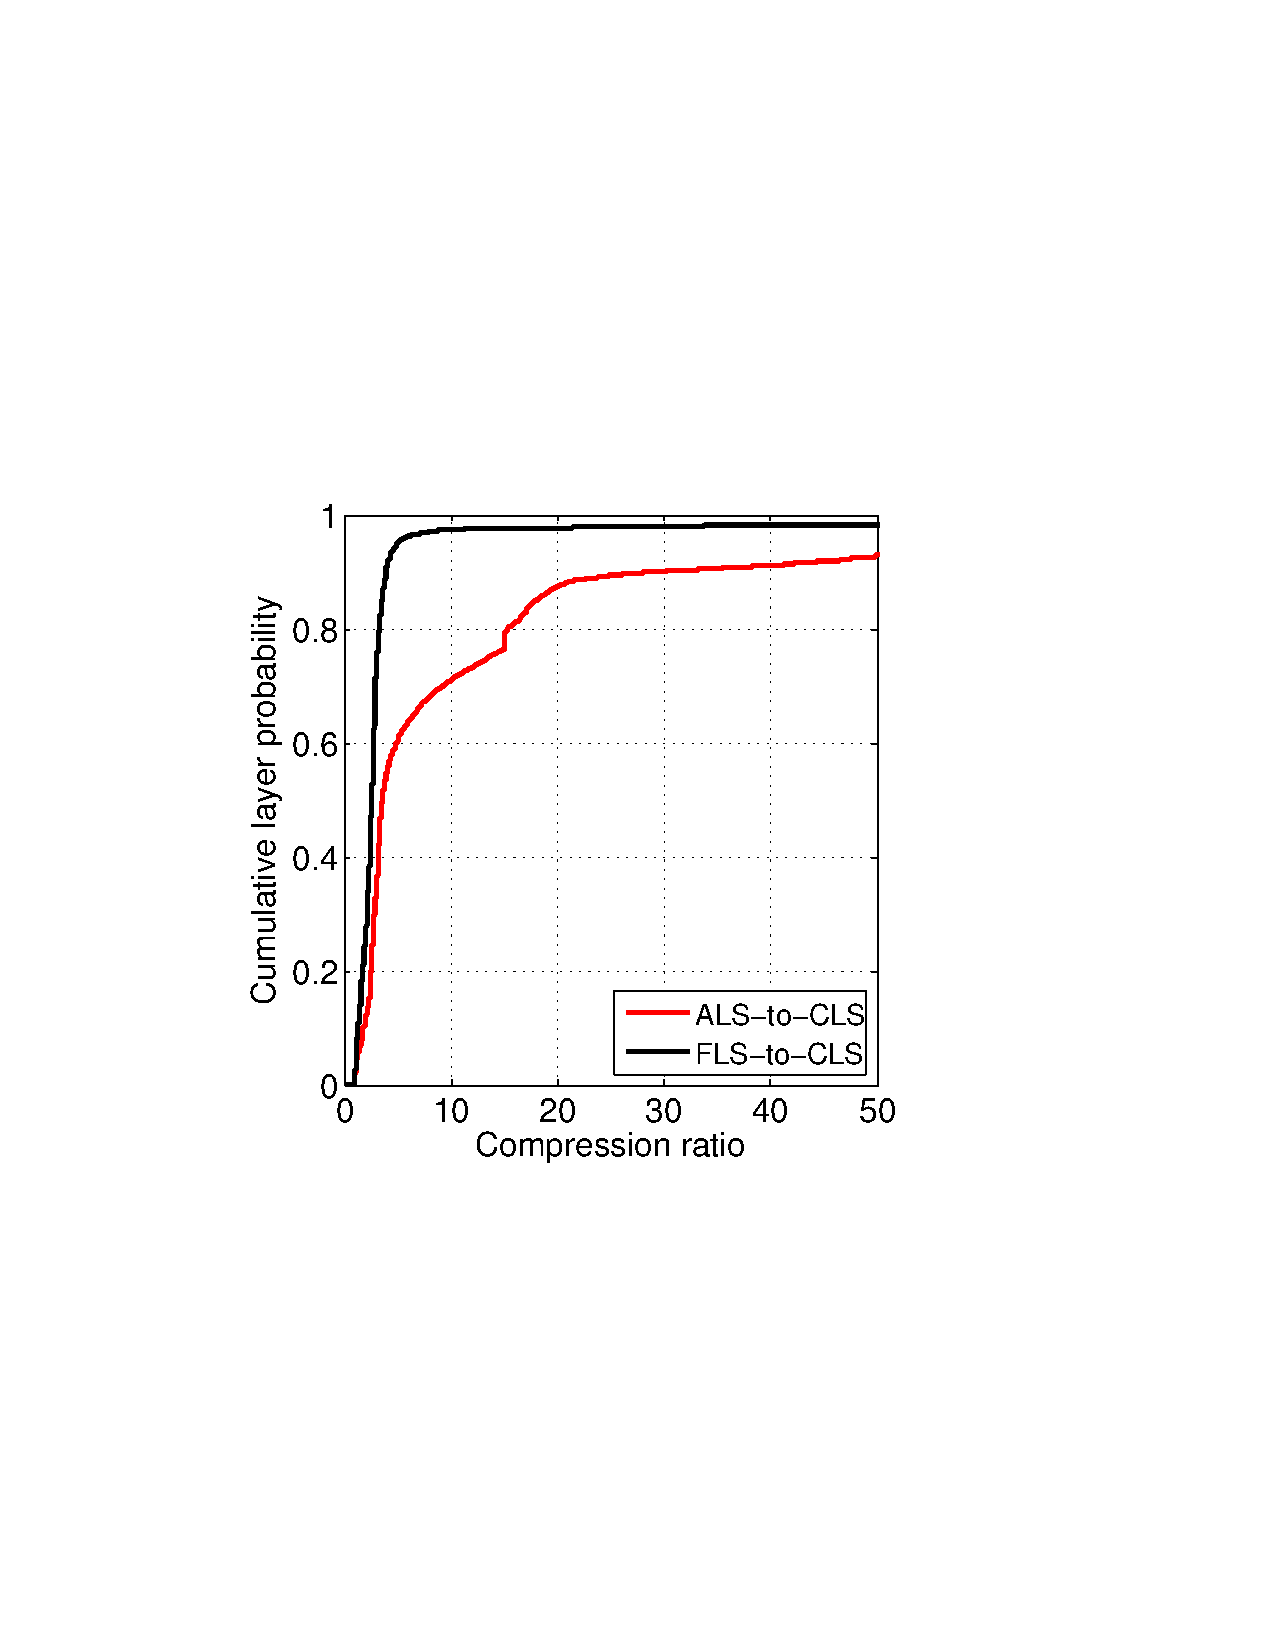
\includegraphics[width=0.23\textwidth]{graphs/cdf_compression_ratio.pdf}
	}
	\subfigure[Histogram of comp. ratios]{\label{fig_his_compression_ratio}
		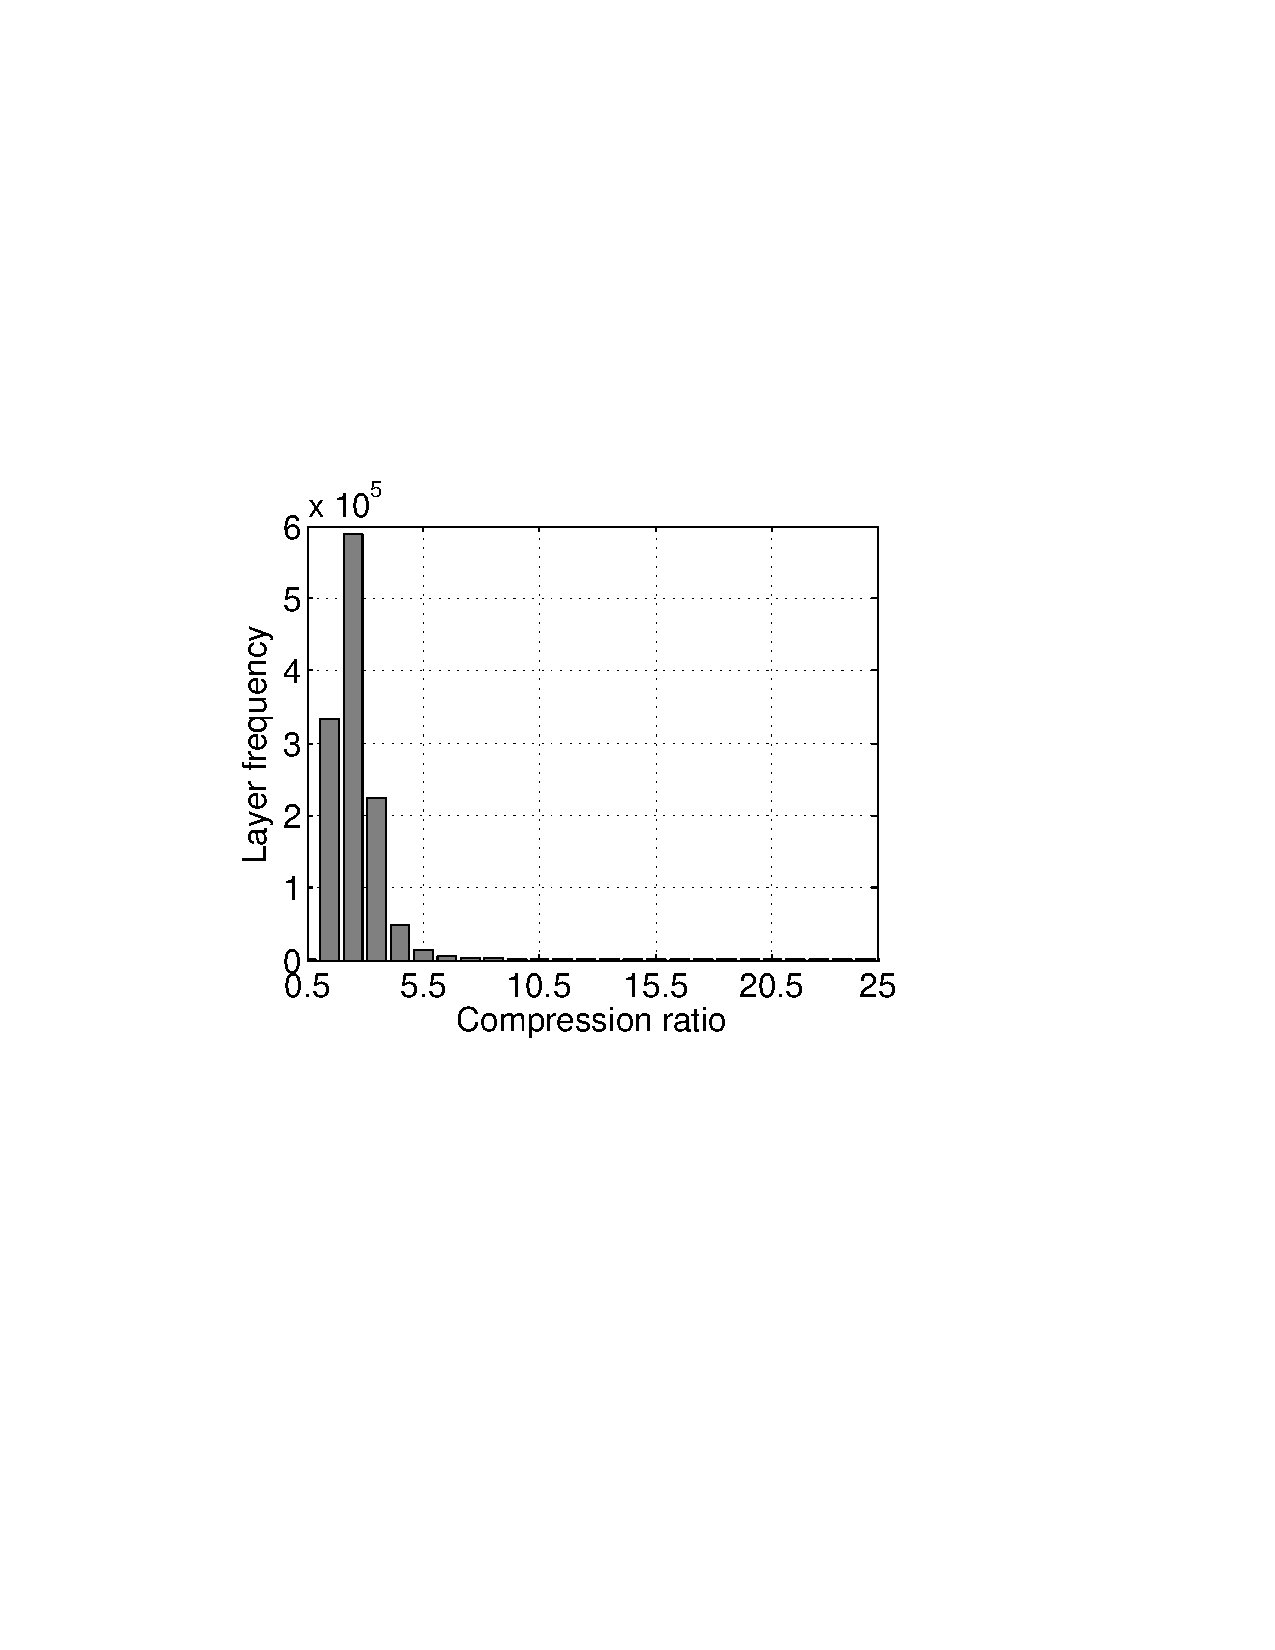
\includegraphics[width=0.223\textwidth]{graphs/his_compression_ratio.pdf}
	}
	\caption{Layer compression ratio distribution
	%\vcomment{Different colors are used in figure (a) and (b) FLS/CLS\nancomment{will address later}}
	}
	\label{fig-compression-ratio}
\end{figure}


%\paragraph{Layer compression ratios}

\subsection{File characterization}

After analyzing layers and images, we conducted a deeper analysis on the files that are stored in containers.% by compressing and upacking the layer 
Specifically, we characterize files in terms of size and type.   
%present file size distribution and clustering file types.
%In this section, we present our redundant file characterization on file repeat count 
Based on this characterization, we create three-level classification hierarchy as shown in Figure~\ref{fig:file-type-hierarchy}.
At the highest level, we created two categories: \textit{Common used file types and non-common used file types} based on the total file size for each type. 
Totally, we got around 1,500 types after analyzing our whole dataset. 
We found that only 133 file types's total redundant file sizes are greater than 5 GB, which take up to 98.4\% files with 166.8 TB totally. We put these 133 file types into high redundant file type group and the remaining files into low redundant file types. Our further classification expands on the 98.4\% common redundant file types. 
%
%are common file types that consists of a largest number of redundant files with large storage space consumed, such as xxx and xxx. 
%Only xxxx\% files are non-common file types that only contains a small number of redundant files with less storage space, such as xxxx and xxxx. 

At the second level of the hierarchy, we clustered high redundant file types based on the \textit{major file format, usage or platform} involved by each file type. We identified redundant files' types relevant to \textit{EOF (executable, object code, and libraries), source code, scripts, documents, archival, images, databases, and others}.

At the third level, we present the specific redundant file types which take a large percentage of redundant files or storage space.

\subsection{File type}

\begin{figure*}
	\centering
	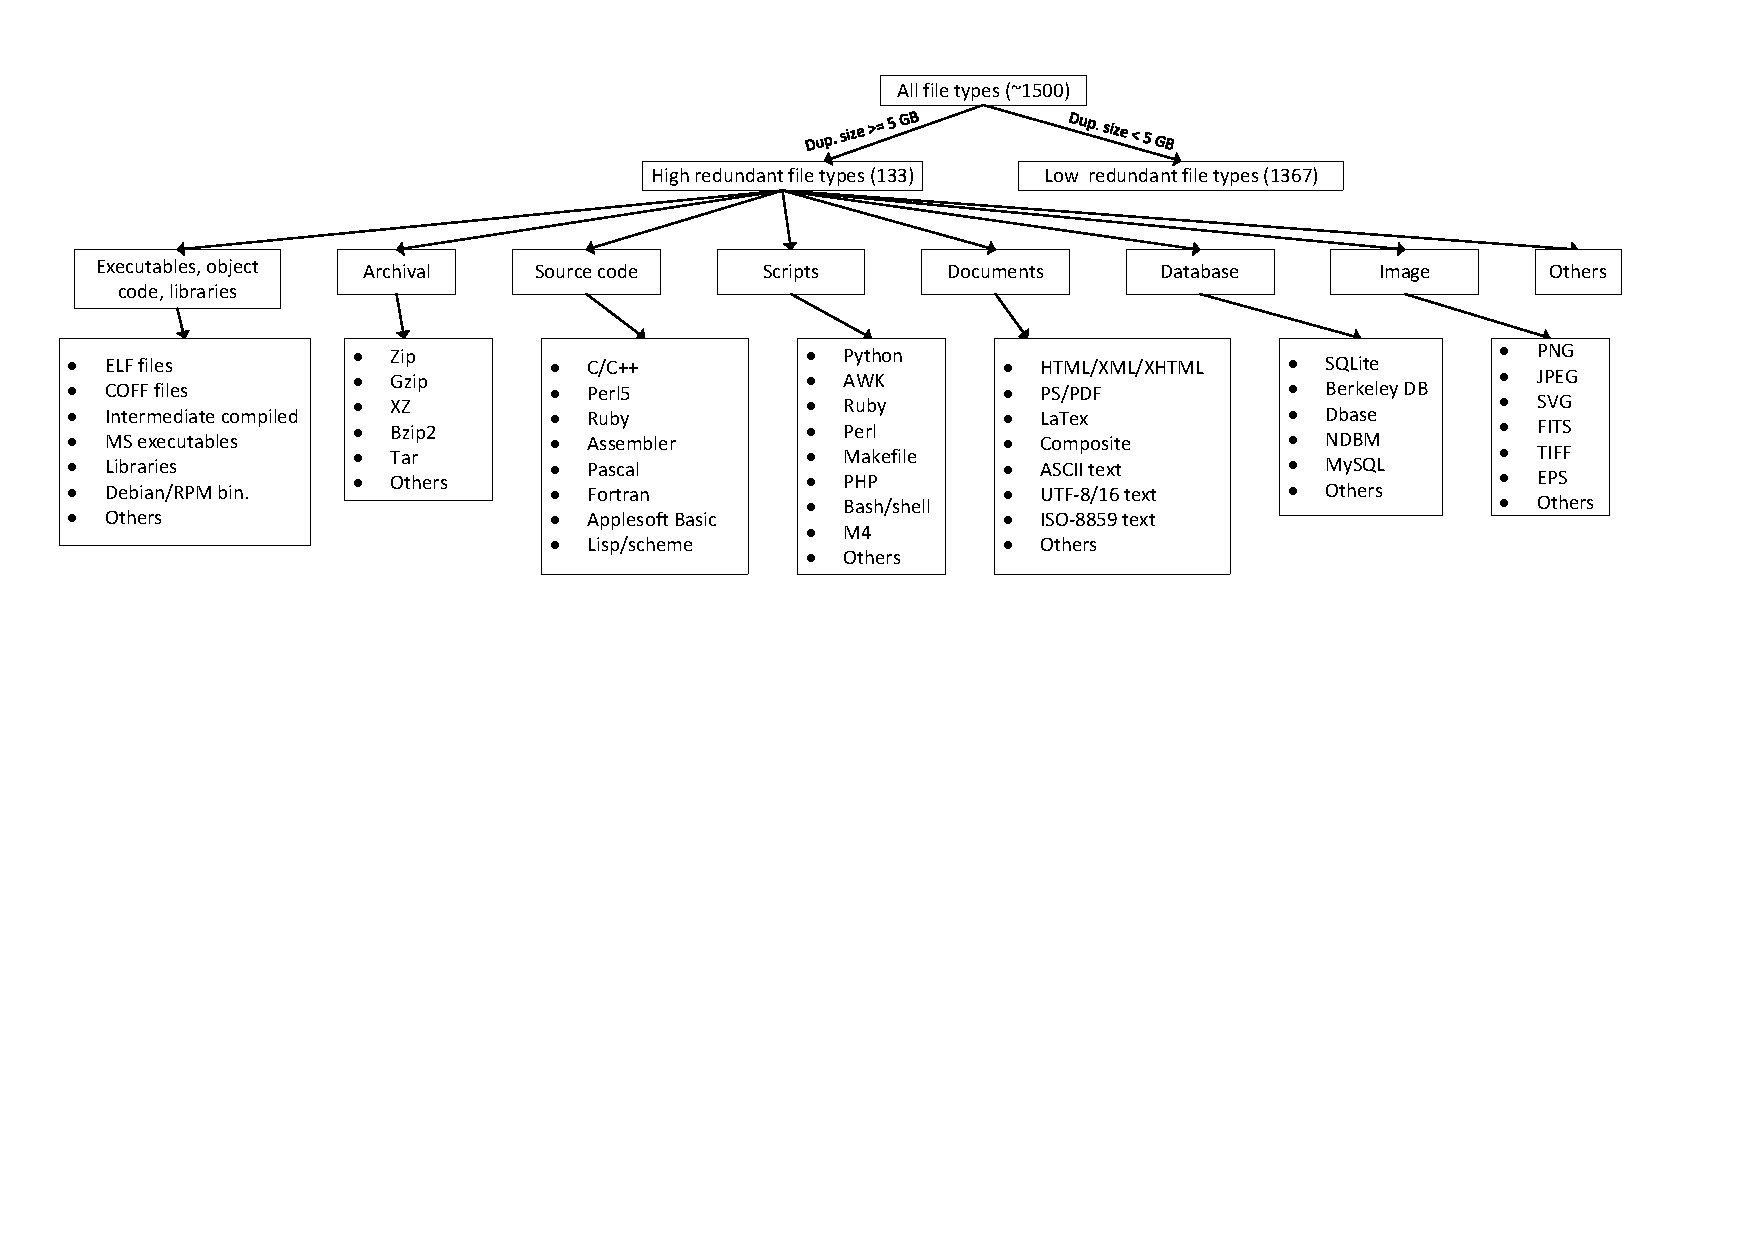
\includegraphics[width=1\textwidth]{graphs/graph-types-hierarchy}
	\caption{Taxonomy of file types.
	}
	\label{fig:file-type-hierarchy}
\end{figure*}


% or further classify the redundant files based on involved by each file type. 
%We selected the file types which take largest storage space.

\paragraph{File size}

\begin{figure}
	\centering
	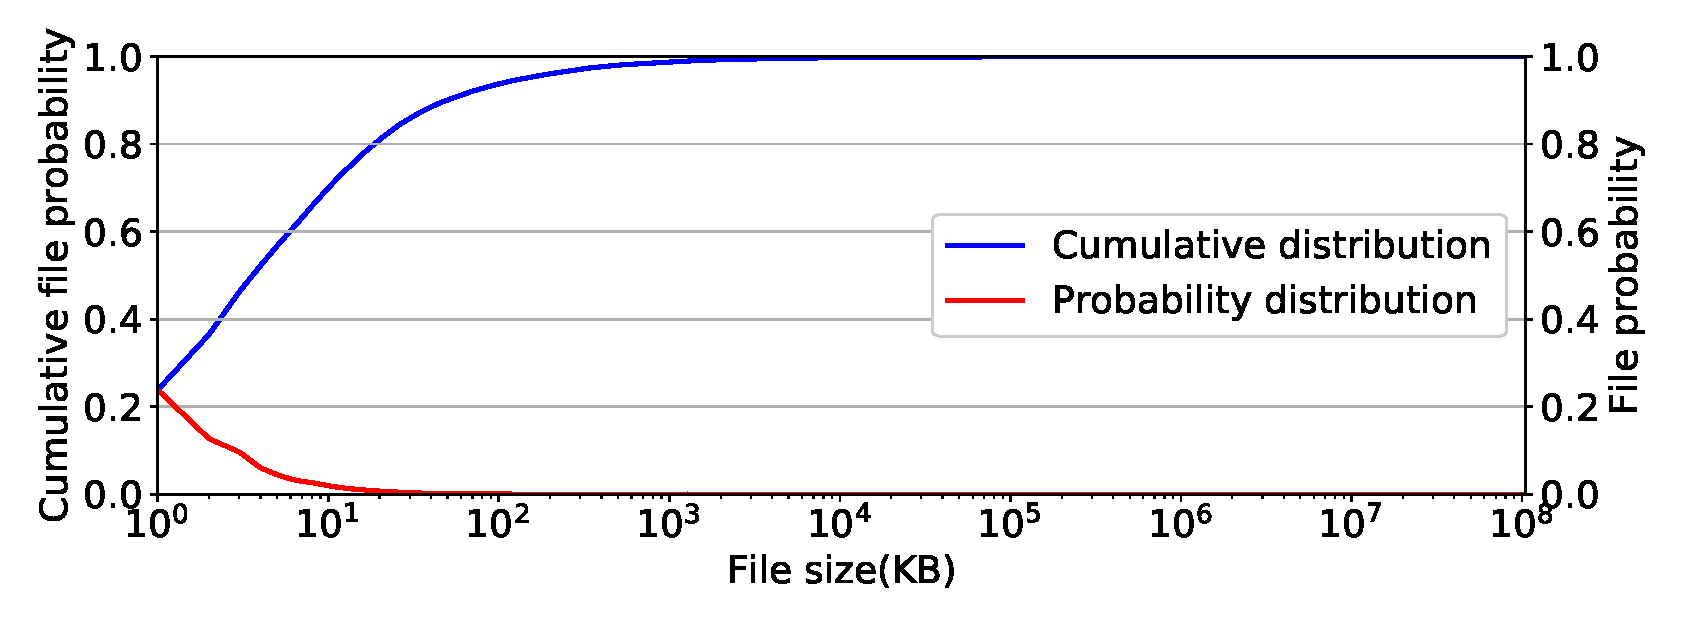
\includegraphics[width=0.5\textwidth]{graphs/File_size-KB.eps}
	\caption{File size distribution.
	}
	\label{fig:file-size}
\end{figure}

Figure~\ref{fig:file-size} shows cumulative and probability distribution of file size.
%of unique dataset after we remove the redundant files.
\textit{Most files are smaller files.} For example, 91\% files are equal or less than 100 KB. 
Around 22\% of files are less than 1 KB. 
\textit{This is consistent with our finding that the layer size and image size are small both in compressed and uncompressed format.}  


%\subsection{File repeat count}
%\subsection{File size}


%As shown in Table~\ref{fig_image_growth}, the number of repositories increased
%linearly during our observation period from May 30th to September 20th,
%2017. Note that the graph shows a gap of 15 days due to Docker Hub changing the way it
%indexes repositories. The total number of repositories
%grew from 633,915 to 687,292, resulting in an average creation rate of 1,241
%repositories per day.
%This rapid growth of repositories suggests that storage optimizations will
%be crucial for registries in the neear future.
%Notice also,
%that each repository contains multiple tagged images and, therefore, we 
%significantly underestimatet the size of Docker Hub's content.



%\section{Deduplication analysis}
\label{sec:redundant_files}
%\NZ{I would like to add some general analysis before dedup analysis.}
In this section, we investigate the potential for data deduplication in the
Docker registry.
%
We first analyze the benefits of data reduction
techniques that Docker already implements---layer sharing and local
compression.
%
\LR{We should introduce the term layer-level deduplication in the previous
section.}
%
\VT{Lukas, I rephrased and changed to layer sharing, which was introduced in
prev. section. c if it reads better now.}
\NZ{changed to layer-sharing.}
%
%Docker, in its current state, already performs rudimentary deduplication by
%sharing identical layers between images.
%
%We start our analysis from quantifying how much benefits does this existing
%approach provides.
%
%However, we believe that there is significantly more potential in
%deduplicating individual files in the layers.
%
We then use the same dataset to estimate the efficacy of file-level
deduplication and analyze the root causes of the high file redundancy found
across container images.
%

\section{Methodology}
\label{sec:methodology}


%%%%%%%%%%%%%%%%%%%%%%%%%%%%%%%%%%%%%%%%%%%stats for old dataset%%%%%%%%%%%%%%%%%%%%%%%%%%%%%%%%%%%%%%%%%%%
\begin{table*}
	\centering
	\caption{Dataset summary} \label{tab-dataset-summary}
	\begin{tabular}{c|c|c|c|c|c|c}%p{0.14\textwidth}
		\hline
		% after \\: \hline or \cline{col1-col2} \cline{col3-col4} ...
		Num. of images crawled & Num. of unique images    & Num. of images downloaded  & Num. of layers downloaded \\
		\hline
		634,412                 & 457,627                 & 346,243                    & 1,763,354  \\
		\hline
		Num. of images analyzed & Num. of layers analyzed & Compressed dataset size              &  Num. of files totally \\
		\hline
		319,620                     & 1,607,533                     & 51TB                        & 117,665,791  \\
		\hline
	\end{tabular}
\end{table*}

%%%%%%%%%%%%%%%%%%%%%%%%%%%%%%%%%%%%%%%%%%%stats for new dataset%%%%%%%%%%%%%%%%%%%%%%%%%%%%%%%%%%%%%%%%%%%
%\begin{table*}
%	\centering
%	\caption{Dataset summary} \label{tab-dataset-summary}
%	\begin{tabular}{c|c|c|c|c|c|c}%p{0.14\textwidth}
%		\hline
%		% after \\: \hline or \cline{col1-col2} \cline{col3-col4} ...
%		Num. of images crawled & Num. of unique images    & Num. of images downloaded  & Num. of layers downloaded \\
%		\hline
%		634,412                 & 457,627                 & 346,243                    & 1,763,354  \\
%		\hline
%		Num. of images analyzed & Num. of layers analyzed & Compressed dataset size              &  Uncompressed dataset size \\
%		\hline
%		344,056                     & 1,748,089                     & 51TB                        & xxx  \\
%		\hline
%	\end{tabular}
%\end{table*}

In this section we describe our methodology for:
%
(1)~obtaining a representative Docker image dataset, and
%
(2)~analyzing basic and deduplication properties of the dataset.

%
\begin{figure}
	\centering
	% Requires \usepackage{graphicx}
	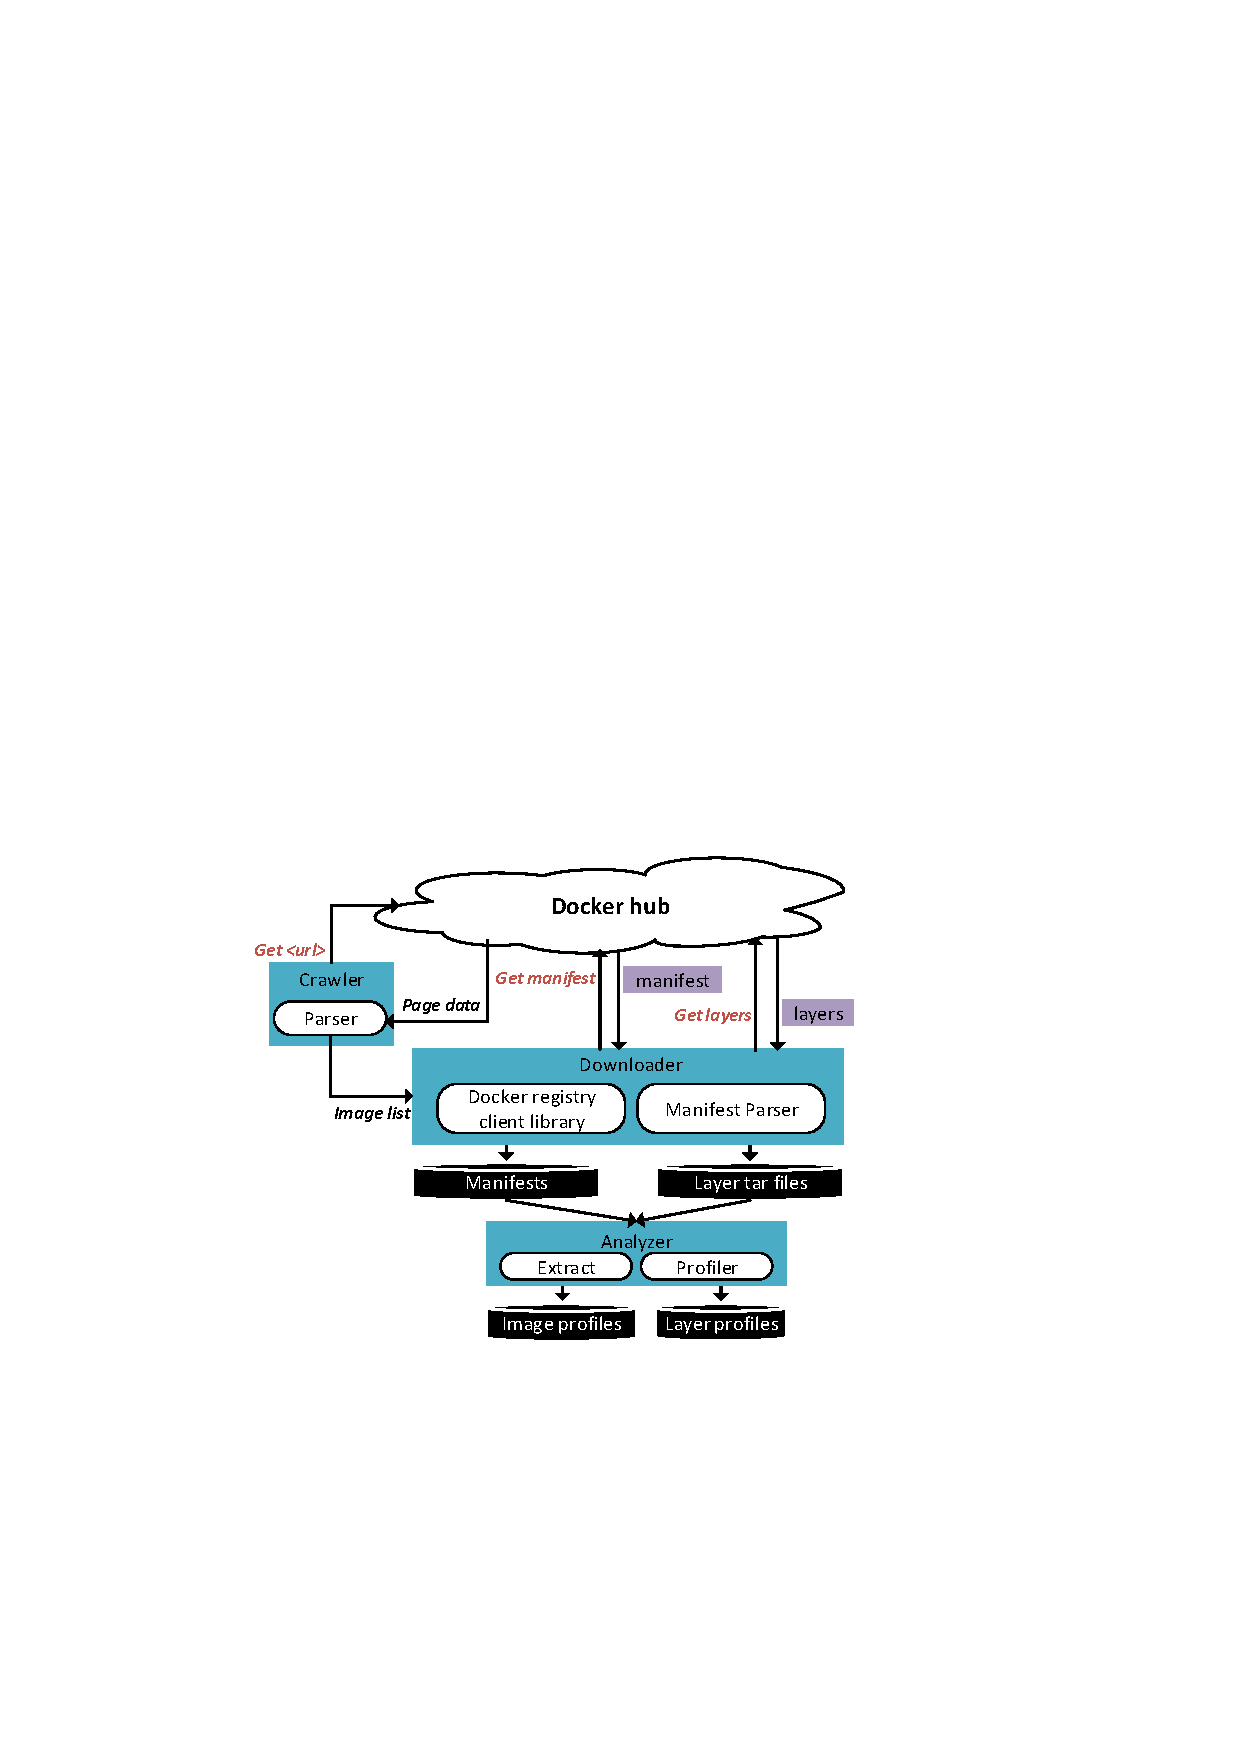
\includegraphics[width=0.5\textwidth]{graphs/fig-downloader-analyzer.pdf}\\
	\caption{Crawler, Downloader, and Analyzer
		%\vcomment{Can we add colors to this figure? Also, increase the font a bit.}
	}
	\label{fig-downloader-analyzer}
\end{figure}

\subsection{Dataset acquisition}
\label{sec:crawler}

We chose Docker Hub~\cite{docker-hub} to download a representative dataset
because (1) Docker Hub is a popular Docker registry for developers to store and
distribute Docker images, and (2) Docker Hub contains a large amount of
\emph{public} Docker images that are available for developers to download for
free.
%
We believe Docker Hub dataset is representative of other registry deployments.

To download a representative dataset from Docker Hub, web crawling is needed
because Docker Hub does not provide an API to retrieve all repository names.
%
Specifically, there are two steps: i)~crawl Docker Hub web pages to list all
repositories; ii)~download the \textit{latest} image (and referenced layers)
from each repository based on the crawler results.
%
Here, we chose latest image from each repository because (1)~the ``latest''
version is usually the newest, stable, and commonly pulled by developers;
(2)~downloading only the ``latest'' version can shorten our downloading process
since the latest images already took about 30 days to download.
%
We plan to extend our analysis to other, non-``latest'', images in the future.

\paragraph{Web crawler}

Public repositories in Docker Hub are divided into official
repositories---served by the Docker Hub partners---and non-official
repositories---provided by regular users and third-party organizations.
%
The number official repositories is less than 200, while, the majority of
repositories in Docker Hub are non-official (over 400 thousand).
%
To list non-official repositories, our crawler utilizes the Docker Hub
web-based search engine to find all available repositories.
%
As the name of non-official repositories is comprised of the user name and the
repository name separated by a ``/'', we can search for ``/'' and obtain a list
of all non-official repositories.
%
The Crawler downloads all pages from the search results and parses the web
content to build a list of all non-official repositories.
%
We ran the crawler on May 30th, 2017 and it produced a list of 634,412
repositories.
%
After removing duplicate entries (introduced by Docker Hub indexing logic), the
final repository list consists of 457,627 distinct repositories.

\paragraph{Downloader}

Instead of using the Docker client to download images, we implement our own
downloader, which calls the Docker registry API
directly~\cite{dockerregistryclient} to download manifests and image layers in
parallel.
%
Our downloader runs significantly faster than a \texttt{docker pull}-based
downloader because the latter one performs other operations besides downloading
the image, such as unpacking the layers and creating the corresponding
read-only snapshots.
%
Our downloader can download multiple images simultaneously and fetch the
individual layers of an image in parallel.
%
Layers are transferred as gzip compressed tar archives.
%
Overall, we downloaded 51~TB of data in 355,319 image manifests with 1,792,609
compressed layers. A total of 111,384 images could not be downloaded mainly because they did not have the \texttt{latest} tag. 
%
\vcomment{Say just one sentence why we did not download some images.}\nancomment{Addressed}
%
Table~\ref{tab-dataset-summary} summarizes the properties of the downloaded
dataset.

%We released both the software that we designed
%to download the images and all profiles we generated
%publicly at {\small{\url{https://elided.for.review}}}.

\subsection{Dataset analysis}

To characterize the dataset perform its redundancy analysis, we first created a
profile for each layer and image, then we performed an in-depth analysis by
using Spark~\vcomment{cite}.

\paragraph{Profiler}

For each image and each layer, profiler creates a profile in JSON format.
%
An image profile contains layer IDs, compressed size, archival size, and
compression ratio of image or layer\vcomment{what?}\nancomment{addressed}.
%
To generate a layer profile, profiler first unpacks layer tarball.
%
A layer profile consists of: (1)~layer metadata, such as layer id, compressed
size, archival size, compression ratio, directory count and file count.
%
(2)~for every file in a layer---file name, file content digest, file type, and
file size.\nancomment{add digest algori, type migic library}
%
Totally, we 1,762,639 layer profiles and 355,196 image profiles. A total of 11,130 images cannot be analyzed because their layers reported reported errors during
extraction and could not be analyzed.
%
\vcomment{Explain briefly why we did not analyze all downloaded images and
layers.}\nancomment{addressed}

\paragraph{Spark-based analyzer}

To quickly perform analysis on hundreds of thousands of profiles, we built an
8-nodes HDFS~\vcomment{cite} and Spark~\vcomment{cite} cluster.
%
We stored all the layer and image profiles in HDFS as parquet
files~\vcommnet{cite}.
%
We then performed basic and redundancy analysis using Spark SQL
module~\vcomment{cite}.
%
For example, for deduplication analysis, we first query unique file content
digests and redundant file content digests along with their repeat counts and
sizes from the layer and image parquet tables.
%
We then calculate corresponding deduplication ratios, as detailed in
Section~\vcomment{ref}.

%and investigated the following questions (RQs):  

%\paragraph{RQ1: What are the redundant ratio of layers and images?}
%
%
%\paragraph{RQ2: What are the redundant files \& why there are so many redundant files?}
%%\nancomment{how to get file type?}
%
%\paragraph{RQ3: How to reduce the redundant files?}
%\nancomment{how to prototype?}

%%%%%%%%%%%%%%%%%%%%%%%%%%%%%%%%%%%%%%%%%%%%%%%%%%%%%%%%%%%%%%%%%%%%%%%%%%%%%%
%                                                                            %
%                                OLD METHO                                   %
%                                                                            %
%%%%%%%%%%%%%%%%%%%%%%%%%%%%%%%%%%%%%%%%%%%%%%%%%%%%%%%%%%%%%%%%%%%%%%%%%%%%%%
%%\nancomment{
%%	TODO: \\
%%	1. Complete fig and table\\
%%}
%
%\lrcomment{ I think in general it would be good if we emphasize in this section, what
%was challenging about downloading all this data and how the presented approach
%overcame these challenges. \nancomment{challenges include: 1. obtaining a list of all the repositories in docker hub; 2. effectively downloading all the images. 3. indept analysis}}
%
%Our methodology consists of three steps~(Figure~\ref{fig-downloader-analyzer}):
%1)~crawl Docker Hub to list all official and nonofficial repositories;
%2)~download the latest image (and referenced layers) from each repository based
%on the crawler results; 3) unpack and analyze images and layers.
%
%%
%%
%%The first step is to massively download the Docker images from Docker registry.
%%
%%When the images are downloaded, we analyze them and calculate statistics distribution for
%%different metrics.
%%
%%The details of each step are covered in the following sections.
%%
%%\vcomment{I suggest to restructure this section simirarly to background to
%%revolve around the figure. Once you add the diagram describing our methodology
%%(like we put on the whiteboard ones), start describing components on it in the
%%order they are used: crawler, downloader, analyzer. Having two subsection:
%%``downloader'' and ``downloading images'' is confusing.
%%
%%We might want to have less deep structure also:
%%
%%3. Methodology
%%  (Figure)
%%3.1 Crawler
%%3.2 Downloader
%%3.3 Analyzer
%%}
%%
%%\nancomment{addressed}
%
%%\nancomment{
%%	figures are stored in google drive, the link is pinned in slacker;
%%	%https://drive.google.com/open?id=0B4jePsYXW6SSTTRLb0FHVXVjNUk
%%	figures/fig-docker-architecture.pdf}\\
%
%
\begin{figure}
	\centering
	% Requires \usepackage{graphicx}
	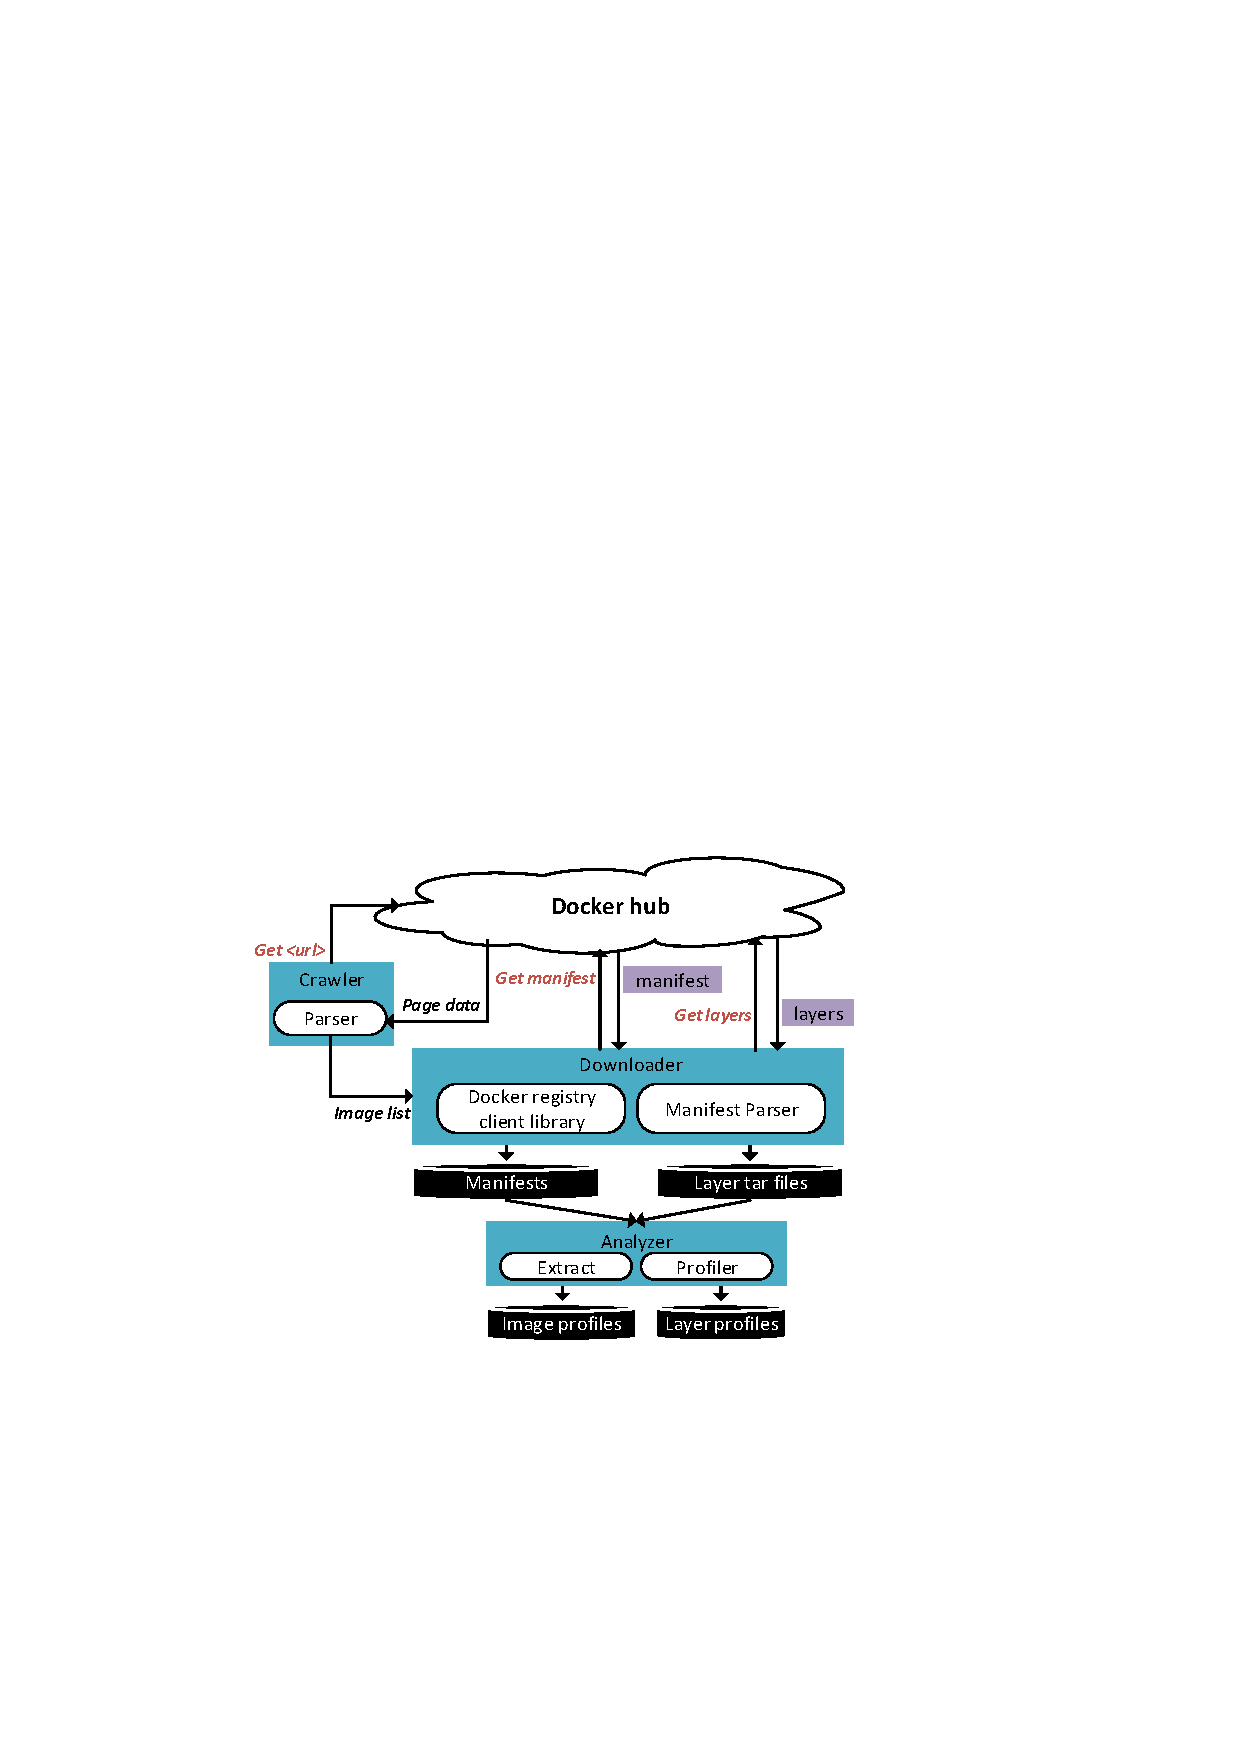
\includegraphics[width=0.5\textwidth]{graphs/fig-downloader-analyzer.pdf}\\
	\caption{Crawler, Downloader, and Analyzer
		%\vcomment{Can we add colors to this figure? Also, increase the font a bit.}
	}
	\label{fig-downloader-analyzer}
\end{figure}
%
%%how container deameon.
%%
%\subsection{Crawler}
%\label{sec:crawler}
%
%%
%To download a particular image, %or set of images (i.e., a repository)
%the name of the repository name which the image belongs to should be provided.
%The crawler is responsible
%for generating a list of repositories for the downloader.
%%as mentioned in Section~\ref{sec:docker-registry}. 
%%
%%
%%
%%\vcomment{Here and in the whole text we need to be very carefull distinguishing names 
%%of repository and image. Also discussion on image tags is missing, should be in
%%background section.}
%%\nancomment{addressed.}
%%
%Public repositories in Docker registry are divided into official
%repositories---served by the Docker Hub's partners---and non-official
%repositories---provided
%by regular users and third-party organizations.
%%, where For example, official repository Ubuntu Here is an example of the shared 
%%repository official repository Ubuntu and one of its tags. 
%%
%%A repository is a set of Docker images. A repository can be shared by pushing it to a
%%registry server. 
%%Public repositories in Docker registry can be divided into official images and non-official 
%%images.
%%
%The number official repositories is less than 200,
%% The list of official repositories
%%can be retrieved via \lrcomment{add how to list official repos}
%while, the majority
%of repositories in Docker Hub (about 400 thousands)
%are non-official.
%% (around \lrcomment{add number}).
%Listing non-official repositories requires web crawling because
%%to the best of our knowledge,
%Docker Hub does not provide an API to retrieve all repository names.
%
%Therefore, we implemented a Crawler to crawl Docker Hub and list all non-official
%repositories.
%%
%Docker Hub provides a search engine which indexes public repositories and allows
%users to search for a repository according to
%some search string. 
%%
%As the name of non-official repositories is comprised
%of the user name and the repository name separated by a ``/'',
%we can search for ``/'' and obtain a list of all non-official
%repositories.
%%``$\langle namespace\rangle/\langle repository name \rangle $", where~\textit{namespace}
%%is the user name. 
%%
%%In this case, we search for `/' and obtain a list of repositories which contains '/'.
%%
%%In other words, this method lists all the non-official public repositories in Docker Hub.
%%
%The Crawler downloads all pages from the search result.
%%
%Once web pages are downloaded, it parses the web content to build a list of
%all non-official repositories.
%
%%\lrcomment{It may be good to discuss how accurate this method is. Can we miss anything?
%%Can we get wrong results?}
%
%
%
%We ran the crawler on May 30th, 2017 and it delivered a list of 634,412 repositories.
%%
%However, the obtained list contained duplicate entries because 
%the crawling process is not atomic and some repositories have ``/'' in their description.
%%
%After removing all duplicates, the final repository list consists of 457,627
%distinct repositories. 
%%
%
%
%%
%%\vcomment{Explain why, state that it is future work.} 
%%\nancomment{addressed}
%%
%%\vcomment{I'd comment out discussion on '*'---it has low importance.}
%%\nancomment{addressed. let's comment it now and see how to deal with this issue}
%%Note that the namespace of official images is `\textit{library}'.
%%
%
%\subsection{Downloader}
%\label{sec:downloader}
%
%Docker repository is a set of images labeled with \emph{version tags}.
%%The different images in the repository are labeled with tags.
%%
%For example, \texttt{ubuntu:17.10} refers to image version \texttt{17.10} in the
%\texttt{ubuntu} repository.
%%
%If user does not provide a tag when pulling an image, 
%Docker daemon uses the \texttt{:latest} tag by default.
%For example, \texttt{docker pull ubuntu} command pulls the
%\texttt{ubuntu:latest} image.
%%
%In this work we only download images with the \texttt{:latest} tag to
%make the analysis more feasible.  We believe that the latest
%images versions represent most up-to-date state of  Docker images
%%
%and plan to analyze images with other tags in the future.
%
%
%
%%The downloader takes the list from the crawler as an input and retrieves
%%all the listed images from Docker Hub (see Figure~\ref{fig-downloader-analyzer}).
%%
%Instead of using Docker CLI to download images,
%%via the Docker Engine,
%we wrote our own downloader that calls Docker registry API directly.
%We used Docker registry client~\vcomment{insert the name, \nancomment{it is called Docker registry client}} library~\cite{dockerregistryclient} to simultaneously
%download \emph{original} manifests and image layers. \lrcomment{What does
%`original' mean here? \nancomment{without any modification}}
%%
%%\vcomment{Should we mention and cite the library that we used here?}
%%
%%\nancomment{addressed (cited in the following para)}
%%
%%
%%We decided to implement a separate downloader due to several reasons:
%%
%Our downloader runs significantly
%faster than \texttt{docker pull}-based downloader
%because the latter one performs
%operations other than downloading the
%image.
%%such as extracting
%%tar archive files and converting manifest version. 
%%
%For example, it automatically extracts each layer's tar archive file
%and creates corresponding read-only snapshot with  configured Docker storage driver.
%%and converts the manifests that are schema version 1 to schema version 2
%%(starting from Docker engine version 1.10).
%This
%not only takes considerable amount of time but also leads
%to overly high storage space utilization.
%%
%% affects
%%our results about manifest version statistics;
%%
%Furthermore, the local storage format of Docker client makes it difficult
%to analyze the contents of each layer separately.
%%Second, layer content directories are not visible for some Docker storage
%%drivers, e.g., devicemapper, which is not feasible to analyze the layer
%%content. 
%%
%%\vcomment{I think most importantly it is faster because we do not need to
%%perform extra steps that Docker client performs.}
%%\nancomment{addressed}
%%
%
%Our downloader can download multiple images simultaneously and fetch
%the individual layers of an image in parallel.
%%within each image downloading process, layers are downloaded in parallel.
%%
%%To download the original manifests and layers from Docker Hub, downloader
%%embeds a library called Docker registry client API citeXXX which only encapsulates
%%manifest and layer downloading functions in Docker engine without extracting layer
%%tarball and converting manifest version. 
%%
%%
%%\subsubsection{Downloading images}
%%
%%\vcomment{definitely need to merge this subsection with Downloader subsection.
%%See my comment for the whole section.}
%%\nancomment{addressed}
%%
%%As shown in Figure~\ref{fig-downloader-analyzer}, downloader first obtains a 
%%list of public images through crawling Docker Hub.
%%
%%Then, it starts downloading process.
%%
%%It mainly downloads two components: manifest and individual layer files. 
%The process consists of two steps.
%%
%First, fetching the manifest by sending a \texttt{GET} request to
%$/v2/\langle name \rangle/manifests/\langle reference \rangle$,
%where~\textit{name} refers to
%$\langle namespace\rangle/\langle repository name \rangle$
%and \textit{reference} is typically a version $\langle tag \rangle$.
%%
%%
%%\lrcomment{Are the following 4 sentences needed?}
%%Note that the~\textit{namespace} of official is~\textit{library}.
%%
%%The reference can include a tag or digest.
%%
%%Note that currently we only downloaded the images with~\textit{latest} tag to shorten
%%the downloading process. In the future, we will download all the images with different tags.
%%
%%As discussed in Section~\ref{xxx}, manifest consist of multiple layer digests.
%%
%%Note that Schema 2 versioned manifest also contains a config file digest.
%%\vcomment{I believe we never explained what is config file. We need to discuss in
%%in background section.}
%%\lrcomment{Do we use config files in the analysis? If they contain the command
%%to run in the container, I think that could give us some interesting insights into
%%how people use containers.}
%%
%Second, once the manifest is downloaded, the downloader uses the layer digests to
%download individual layers
%%(including the config file for Schema 2 versioned manifest)
%by sending $GET$ request to $/v2/\langle name \rangle/blobs/\langle digest \rangle$.
%\textit{Name}, as for manifests,
%refers to $\langle namespace\rangle/\langle repository name \rangle$
%while~\textit{digest} refers to the layer digest.
%%or config file digest.
%Layers are transferred as gzip compressed tar archives.
%%\vcomment{What compression is used?}
%%\nancomment{addressed}
%
%%
%%\vcomment{I believe different parts of this section belong to different
%%	earlier parts: some to crawler, some to downloader.}
%%\nancomment{addressed}
%%
%
%
%The whole downloading process took around 30 days.
%%
%Overall, we downloaded 51~TB of data in 355,319 image manifests with 1,792,609
%compressed layers.
%%
%A total of 111,384 images could not be downloaded due to three reasons.
%%
%First, 5\% of the images required authentication and
%second, 87\% of the images did not have the \texttt{latest} tag.
%Third, 8\% of the images contains layers that cannot be downloaded.
%% 0.05189255189	0.8666056166 0.0815018315
%%As we discussed in Section~\ref{sec:crawler}, we only downloaded the \texttt{latest}
%%version of an image to shorten the downloading process.
%Table~\ref{tab-dataset-summary} summarizes the properties of downloaded
%dataset.
%
%%\nancomment{2. TODO: add a table discribe:\\
%%	how many images, duplicate ratio\\
%%	how many cannot download, (removed, no latest)\\
%%	how many layers, config, manifest\\
%%	dataset}
%
%%\subsubsection{Docker image dataset statistics}
%
%
%
%%The reason probably is that Docker Hub adjusted websites'order or modified the
%%websites because of the increasing of Docker images during our crawling process.
%%Our crawler has a unavoidable delay between each HTTP requst and HTTP response. 
%%So it couldn't reflect the websites'order or website content changes. Another
%%reason is that search engine lists duplicated images 
%
%%Overall, we downloaded XXX image with XXX layers. Table~\ref{XXX} summaries
%%the statistics of Docker image dataset we downloaded. Then, we profiled the
%%layers, config files, and manifests we downloaded and calculated the statistic
%%distribution for different metrics. 
%
%%Some embedded literal typset code might 
%%look like the following :
%%
%%{\tt \small
%%\begin{verbatim}
%%int wrap_fact(ClientData clientData,
%%              Tcl_Interp *interp,
%%              int argc, char *argv[]) {
%%    int result;
%%    int arg0;
%%    if (argc != 2) {
%%        interp->result = "wrong # args";
%%        return TCL_ERROR;
%%    }
%%    arg0 = atoi(argv[1]);
%%    result = fact(arg0);
%%    sprintf(interp->result,"%d",result);
%%    return TCL_OK;
%%}
%%\end{verbatim}
%%}
%%
%%Now we're going to cite somebody.  Watch for the cite tag.
%%Here it comes~\cite{Chaum1981,Diffie1976}.  The tilde character (\~{})
%%in the source means a non-breaking space.  This way, your reference will
%%always be attached to the word that preceded it, instead of going to the
%%next line.
%
%\begin{table*}
%	\centering
%	\caption{Dataset summary} \label{tab-dataset-summary}
%	\begin{tabular}{c|c|c|c|c|c|c}%p{0.14\textwidth}
%		\hline
%		% after \\: \hline or \cline{col1-col2} \cline{col3-col4} ...
%		Num. of images crawled & Num. of unique images    & Num. of images downloaded  & Num. of layers downloaded \\
%		\hline
%		634,412                 & 457,627                 & 346,243                    & 1,763,354  \\
%		\hline
%		Num. of images analyzed & Num. of layers analyzed & Compressed dataset size              &  Uncompressed dataset size \\
%		\hline
%		344,056                     & 1,748,089                     & 51TB                        & xxx  \\
%		\hline
%	\end{tabular}
%\end{table*}
%
%\subsection{Analyzer}
%\label{sec:analyzer}
%
%The analyzer analyzes extracts downloaded layers
%and analyzes them along with image manifests.
%It creates two types of profiles for each image:
%an image profile and individual layer profiles.
%Each profile contains different metrics for the whole image and
%its individual layers, respectively.
%Profiles are stored in JSON format.
%
%
%%
%%\vcomment{I think we do not need to discuss any metrics above, as you
%%discuss them below in corresponding subsections.}
%%\nancomment{addressed}
%%
%
%\paragraph{Layer profile.}
%
%Layers are downloaded as compressed tar archive files.
%%
%To produce the layer profile, the analyzer first decompresses and extracts each
%layer tarball to a layer directory.
%%
%Then, it recursively traverses each subdirectory and obtains
%the metadata information for each subdirectory.
%
%The layer profile contains metadata about the layer, its directories,
%and files: 
%
%\{
%layer digest; 
%Archived layer size (ALS); 
%Sum of containing file sizes (FLS); 
%Compressed layer size (CLS); 
%ALS-to-CLS (compression ratio);
%FSL-to-CLS (compression ratio);
%Directory count;
%File count;
%Layer directory depth;
%\}
%
%\{
%Directory name;
%Directory depth;
%File count;
%Directory size;
%\}
%
%\{
%File name;
%File digest;
%File type;
%File size;
%\}
%
%\begin{compactitemize}
%	\item XXX
%	\item XXX
%	\item XXX
%	\item XXX
%\end{compactitemize}
%
%%file count while directory metadata covers directory depth and size
%%and file metadata includes size and type. The full set of metrics
%%covered by the layer profile is shown in Table~\ref{xxx}.
%
%
%%Each layer profile contains
%%layer metadata information, such as layer size and file count; and
%%directory metadata information for each subdirectory, such as directory
%%depth and directory size; and file metadata information for each file,
%%such as file size and file type.
%%
%%\vcomment{I'm not sure what figure we want here. I think a table might suffice.}
%%\nancomment{addressed}
%%\nancomment{3. TODO: 
%%	add a fig: discribe all layer metadata, config metadata, and manifest metadata structure} 
%%
%%\nancomment{4. TODO: 
%%	add a table\\
%%	layer tarball format statistics, tar, compressed, non compressed\\
%%	config statistics, txt, json\\
%%	manifest statistics, txt, json}
%\vcomment{Instead of the table, let's us the itemized list above for now, \nancomment{already add table 1. and we dont need to list metrics here since we present them in results}}
%
%
%\paragraph{Image profile.}
%
%To create the image profile, the analyzer parses the manifest
%and obtains the configuration information such as OS and architecture.
%Further, once individual layers are analyzed, the analyzer can build the whole image
%profile by including pointers to its layer profiles. In total, image profile includes
%the following information:
%\{
%Image name; 
%Archived Image size (AIS); 
%Sum of containing file sizes (FIS); 
%Compressed image size (CIS); 
%ALS-to-CLS (compression ratio);
%FSL-to-CLS (compression ratio);
%Directory count;
%File count;
%\}
%
%\begin{compactitemize}
%	\item XXX
%	\item XXX
%	\item XXX
%	\item XXX
%\end{compactitemize}
%
%% image metadata information,
%%such as image pull count and layer count, and image configuration
%%information, such as OS version and architecture. All metrics
%%in the image profile are shown in Table~\ref{xxx}.
%
%%Note that schema version 2 manifests store configuration information in a
%%config file as discussed in Section~\ref{sec-image-layers}.
%%\lrcomment{I think we removed the part about different manifest versions from
%%the background, should add it back.}
%%
%%As shown in table~\ref{xxx}, \gap of manifests are Schema version 2 while the
%%rest are Schema version 1. 
%
%%
%%
%%While layer profile
%%contains layer metadata information, such as layer size and file count;
%%and directory metadata information for each subdirectory, such as directory
%%depth and directory size; and file metadata information for each file, such
%%as file size and file type.
%%
%%Table~\ref{xxx} summaries the layer archive file, config file, and manifest
%%statistics.
%
%
%%\vcomment{This section (and some other places) contain a lot of ``etc.''. The
%%general rul of thumb never to ue etc. in a scientific paper. Instead,
%%say: "e.g.,", or "for example," or "for instance"}
%%\nancomment{addressed}
%%\subsubsection{Config profile}
%

\subsection{Deduplication ratio} 
\label{sec:dedup_ratio}

%In Docker registry, layers are shared among different images to eliminate
%duplicates.  
%
%In this section, we investigate if layer-level content addressable
%is enough for Docker registry to mitigate redundancy.  
%
%Specifically, we look in
%$to the sharing rate of layers across images to calculate how much space is
%aved by using layer-level content addressable storage.  
%
%We also investigate
%that how much redundant data exists across images.

\paragraph{Layer sharing}

\begin{figure}
	\centering
	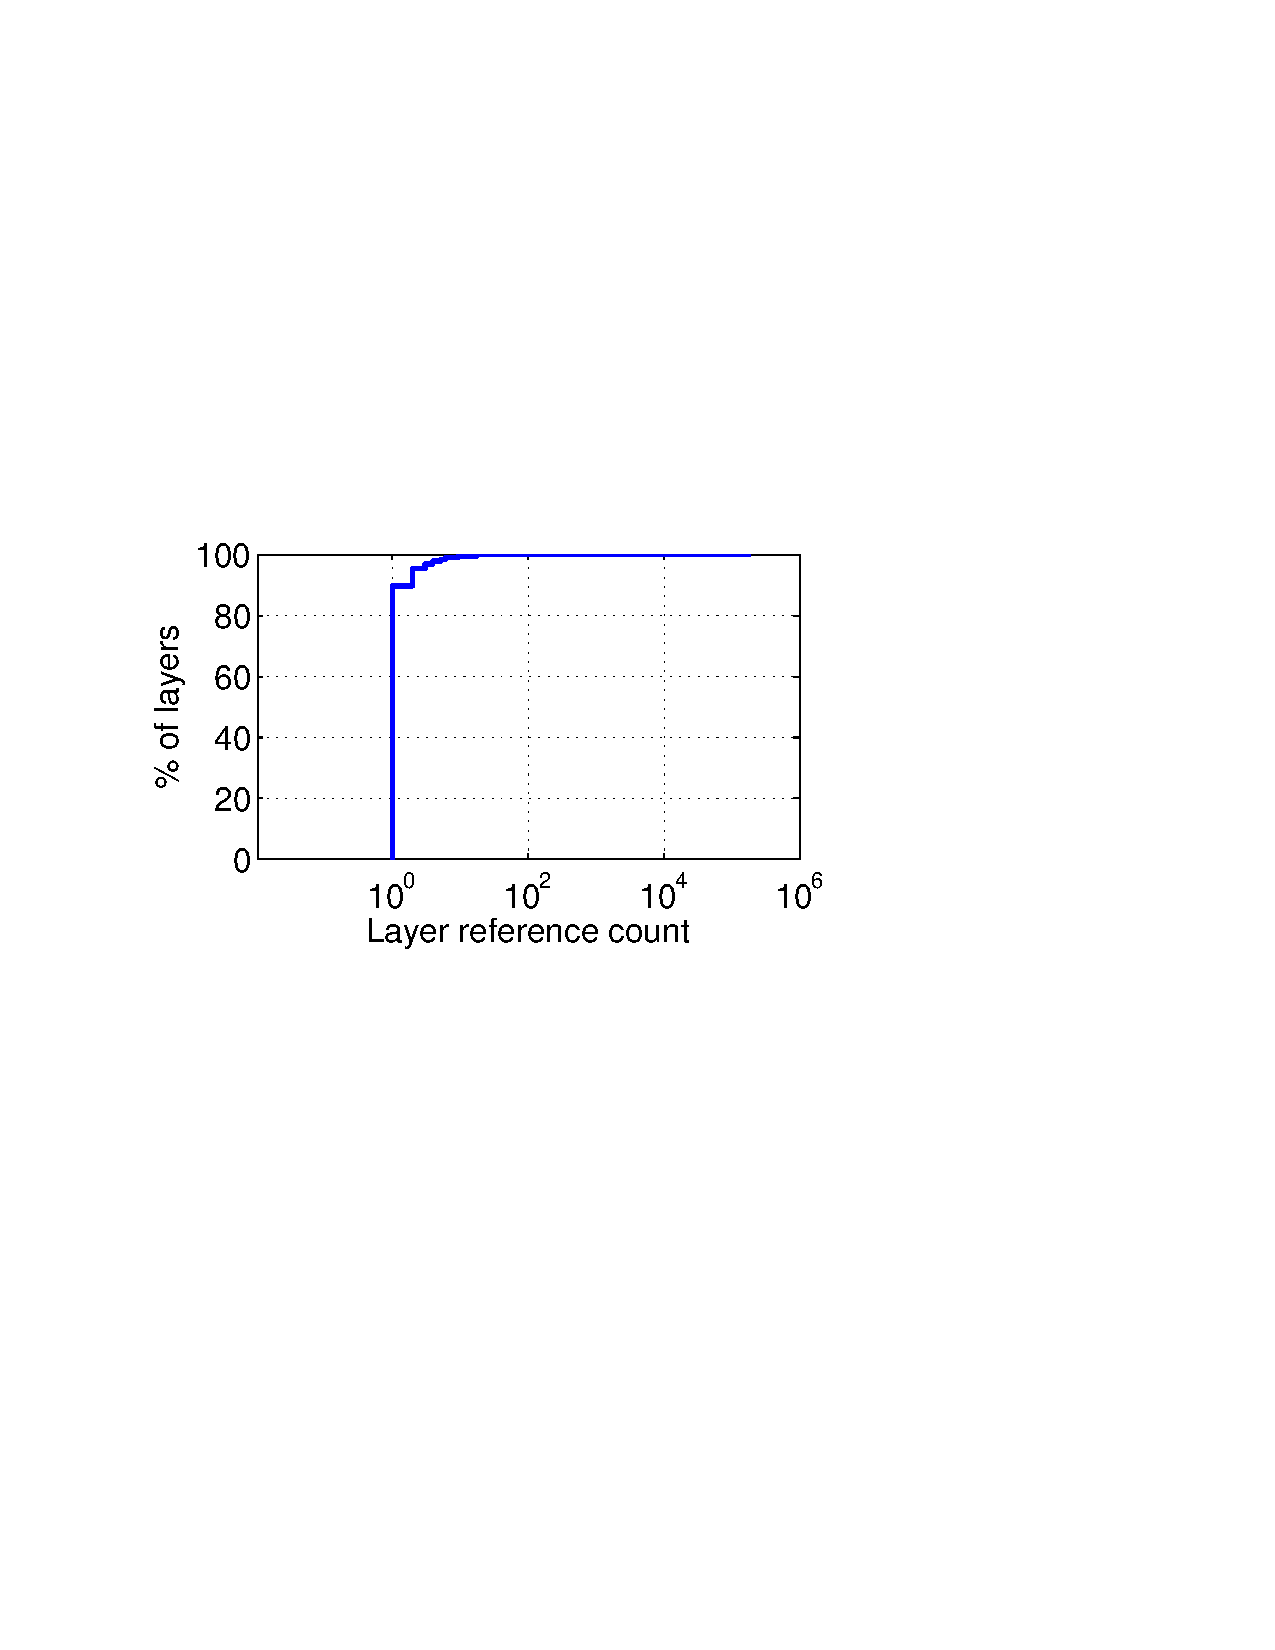
\includegraphics[width=0.21\textwidth]{graphs/shared-cnt-cdf.pdf}
	\caption{CDF of layer reference count.
	}
	\label{fig:ref_count}
\end{figure}


In its simplest implementation Docker would not support layer sharing.
%
Instead, every image would be a single flat archive.
%
In fact, some existing containerization frameworks \VT{cite singularity and
openvz} use flat images.
%
Our estimates show that without layer sharing our dataset would grow from 47TB
to 85TB, resulting in \textbf{1.8$\times$} deduplication ratio.
% 
We further computed for each layer, how many times it is referenced by images.
%
Figure~\ref{fig:ref_count} shows that around 90\% of layers are referenced by
only a single image, additional 5\% are referenced by 2 images, and less than
1\% of the layers are shared by more than 25 images.
%
%Accordingly, we calculated the total storage space consumed before layer-level
%content addressability was adopted, which was 84.75 TB.  Thus the redundant
%ratio achieved by layer-level content addressability is around 1.8.
%
%Figure~\ref{} shows the absolute values, revealing that almost 1.5 million
%images are only referenced once.  \acomment{Figure is missing} While there is
%again a large spectrum of reference counts, the maximum is 33,428, the vast
%majority of layers is not shared. 
%
%This hints that the layer-based approach to improve storage efficiency is
%barely utilized and there is room for improvement in how to construct more
%sharable layers.
%
%\emph{These findings reveal that layer level content addressable store has not
%been very successful and most of the layers that exists in Docker Hub are not
%shared among images.
%
%Hence, there is a dire need of a better redundancy management.}
%
%
Interestingly, there were xxx\% layers that were referenced about 1 million
times.
%
Our investigation showed  that these layers are~\VT{Verify this
sentence and extend with analysis.}

\VT{Use \% instead of probability in all Figures (both # and labels).}

\paragraph{Compressibility}



\paragraph{File-level deduplication}
%As discussed in compression ratio analysis, we see that there is redundant
%data in both layers and images.  We conducted simple form of deduplication to
%Interestingly,
Next, we calculate deduplication ratio in terms of file count and capacity for
the complete uncompressed dataset. %(Table~\ref{tbl:overall-redundant_ratio}).
%the redundant file overhead of the uncompressed dataset 
%
We find that majority of the files have more than one copy (99.42\%), which
take up over 89\% of capacity.
%
\VT{not clear what exactly takes 89\% of capacity}
%
After elimination of file duplicates, the percentage of such files decreases
from 99.42\% to 2.59\%.  
%
\VT{huh? Shouldn't the percentage of duplicate files go to 0?}
%
Overall, only 3.17\% (23.92 TB) of files are unique files while 96.83\% of
files (143.28 TB) are redundant copies. 
%
Correspondingly, the deduplication ratio is 96.83\% and 85.69\% in terms of
file count and capacity, respectively.
%
\VT{let's use $\times$ for dedup ratio, it's conventional}.
%
% Table~\ref{tbl:overall-redundant_ratio} summaries the overall redundant file
% overhead in terms of file count and capacity.
%
\textit{Finding 1: Majority of files in Docker registry are duplicates which
occupy most of capacity, indicating that Docker Hub has severe redundancy
problem.}

%\begin{table} 
	\centering 
	\scriptsize  
	%\begin{minipage}{.5\linewidth}
	\caption{Redundant ratio in terms of file count and capacity}
	\label{tbl:overall-redundant_ratio} 
	\begin{tabular}{|l|l|l|}%p{0.14\textwidth}
		\hline  
		& File count & Capacity \\ 
		\hline 
		Repeat cnt = 1 & 0.58\% & 10.87\%\\
		\hline 
		Repeat cnt $>$ 1 after dedup. & 2.59\% & 3.44\%\\ 
		\hline 
		Repeat cnt $>$ 1 before dedup.  & 99.42\%  & 89.13\%\\ 
		\hline 
		Unique dataset (Uncompressed) & 3.17\% (167,251,437)  &  14.31\% (23.92 TB) \\ 
		\hline 
		Total dataset (Uncompressed) & 5,278,465,130 & 167.20 TB \\ \hline 	
			%\hline 
	\end{tabular} 
\end{table} 


\VT{Move all figures to separate fig- files and tables to tab- files.}

\begin{figure} \centering
	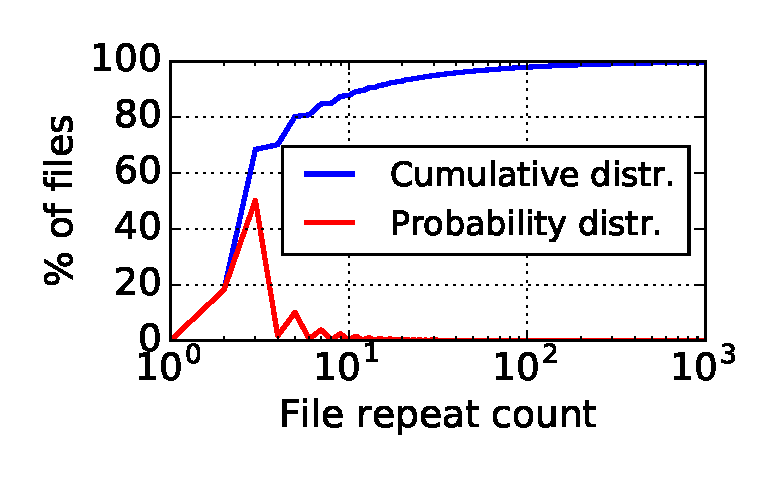
\includegraphics[width=0.45\textwidth]{graphs/File_repeat_count.eps}
	\caption{File repeat count distribution.  } \label{fig:file-repeat-cnt}
\end{figure}

We further analyzed the repeat count for for various files.
%
Figure~\ref{fig:file-repeat-cnt} shows the cumulative and probability
distribution of file repeat count.  
%
We see that over 99.42\% of files have more than one copy.
%
Around 50\% of files have 4 copies and 90\% of files have less or equal than 10
copies. 
%
The file that has the maximum repeat count---\VT{SPECIFY}---is an empty file.
%
\VT{Do we know anything about those empty files}.

\subsection{Deduplication by file types}

\begin{figure} 
	\centering
	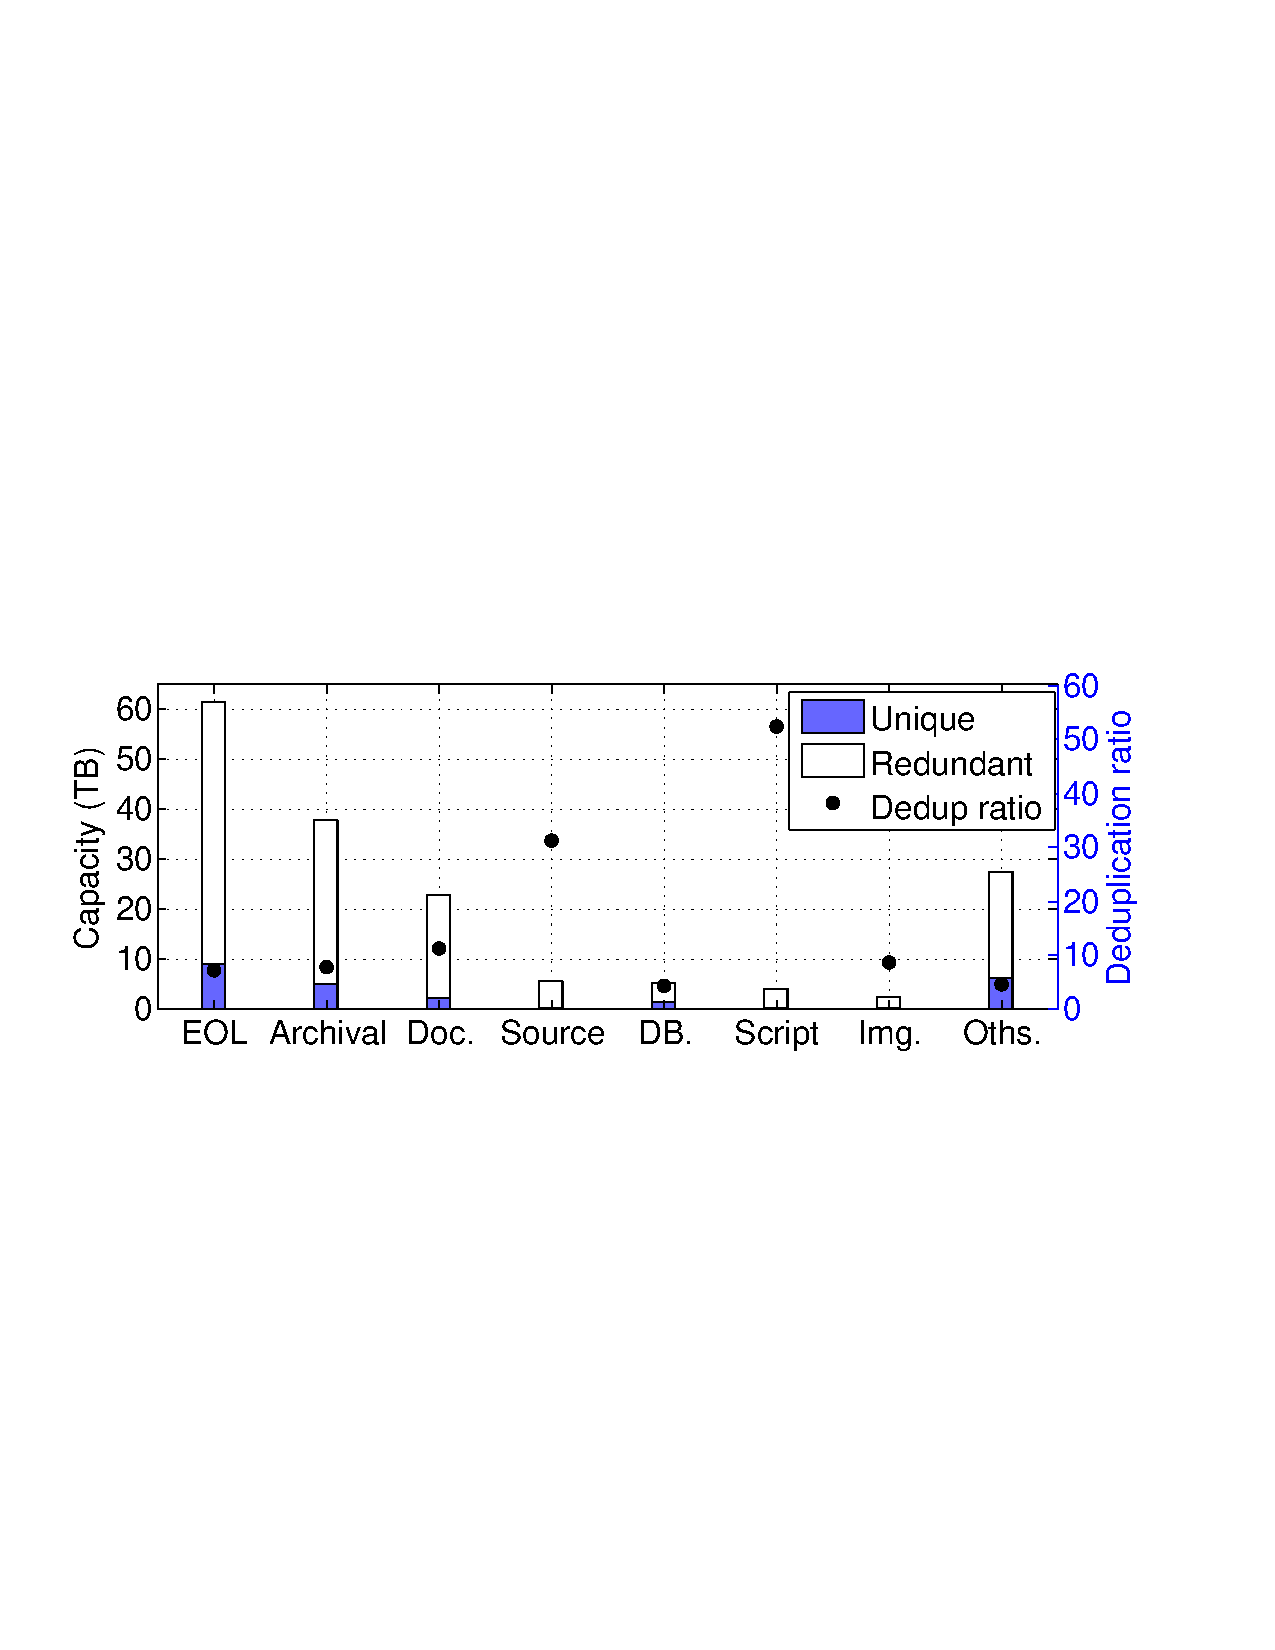
\includegraphics[width=0.45\textwidth]{graphs/dedup-overall} 
	\caption{Deduplication ratio for seven file classes---EOL, archival, documents, source code, database, scripts, images---and other files.
	Light bars indicate the original storage utilization while dark bars represent the capacity after removing redundant files.
	Dots shows the corresponding deduplication ratio.
%
%\VT{Can we stretch X axis to column width to have more space for X-axis labels?}\NZ{addressed}
%%
%\VT{Explain what blue and red bars mean here, as well as dots. Explain
%if dedup ratio is in terms of capacity or file counts.}\NZ{addressed}
%
} 
	\label{fig:dedup-overall} 
\end{figure}




To understand the sources of high data redundancy among Docker images, we
investigate deduplication for common file types.
%
We identify \VT{XXX - how many?} file types (e.g., JPG, C/C++ code, Java files)
using the file type library~\VT{\cite{XXX}} and then group file types into 7
classes by their usage scenarious:
%
1)~executables, libraries, and object files (EOL)
%
\VT{Maybe call them ``Exec.`` instead on the graph and everywhere?}
%
2)~archival,
%
2)~documents,
%
4)~source-code,
%
5)~scripts,
%
6)~images,
%
7)~database files. 
%
\VT{I'd add extensions example in parenthesis for every class. E.g., document is not intuitive.}
These classes consitute 98.4\% of the whole dataset.
%
\VT{Weird, ``Oths'' is ~30TB in the graph, so much more than 1.6\%. What's
going on?}


Figure~\ref{fig:dedup-overall} illustrates the deduplication results for these
classes.
%
The overall deduplication ratio is \textbf{6.99$\times$} and most type classes
have a comparable ratio (see dots in Figure~\ref{fig:dedup-overall}.
%
E.g., the deduplication ratio for EOL files is \textbf{7.14$\times$}.
%
However, source code, scripts, and documents exhibit significantly higher
deduplication ratio--- \textbf{31.25$\times$} for source code,
\textbf{50$\times$} for scripts, and \textbf{12.5$\times$} for documents.
%
This indicates that Docker image builders are prone to frequently replicate
source code, scripts, and documents.
%
%Moreover, the source code and script duplicates generate additional executables
%and object files that are identical.

We found that redundant C/C++ source code takes up over 77\% of the capacity
occupied by source code.
%
Looking closer we found, for example, that Google Test~\cite{googletest}---a
cross-platform C++ test framework available on GitHub~\cite{github}---is
frequently replicated.
%
\DIM{Okay - but could we say something more precise, e.g., what \% of 77\% is
taken by gtest?}
%
Interestingly, we found there are multiple Docker repositories \DIM{Docker
repositories?}\NZ{yes} related to Google Test while there is no official
repository for Google Test.
%
We suspect that many developers replicate open source code from external public
repositories, such as GitHub, and store them in containers.
%
This would also explain the shared source code across different images.
%
\VT{give few more example in addition ot Google Test}


Docker Hub allows developers to automatically build images from
source code in external public repositories and automatically push the built
image to their Docker repositories, we believe that more open source code
may be replicated into different images stored in Docker Hub registry.
%
\VT{I don't understand the last sentence. ``more'' than what?.. And who can 
replicate? don't use passive voice to make it clear.}
%
\textit{To eliminate redundant open source codes in Docker registry in the
future, we suggest that Docker Hub creates offical images for popular
open source codebases so developers can directly pull the image as a
read-only layer}.

Next, we see that EOL files, archival, and images have a similar deduplication
(around \textbf{6.99$\times$}). 
%
Compared with other type classes, the redundant EOL files and archival files
occupy over half of the capacity (51.4\%). 
%
\VT{can we same something where the duplicate archive files come from?.. (Similarly to
Google Test example)}
%
%This is mainly because EOL and archival file sizes are bigger than other type
%group.
% 
Database related files have the lowest deduplication ratio (\textbf{4.2$\times$}),
which contributes little to the overall savings.

All common file types have a high deduplication ratio.  Especially, EOL and
archival files contribute a lot to the overall savings.
%
Also, developers are likely to reuse code rather than create their own.
%
\DIM{Ffrom the data we see there is high source code dedup, but this might be
too much of a generic statement based on this data.}

%We see that 43.15\% of redundant files are documents, 
%%
%Documents have the
%largest number of redundant files (), indicating that users replicate more
%documents than other clusters. While the redundant document files only consume
%14.54\% (20.87 TB) of storage space, indicating that the size of redundant
%document files are small (10.2 KB on average). In comparison, 13.38\% and
%10.23\% of files are EOL files and source codes, which take up over 3.66\%
%(5.3 TB) and 36.85\% (52.9 TB) of redundant storage space, indicating that
%users replicate source codes and create big identical EOF files (108.6 KB on
%average).
%
%Archival files and scripts have almost similarly number of redundant files,
%8.53\% for archival and 8.69\% for scripts. However, archival cluster consumes
%more storage space than that of scripts (32.9 TB for archival and 3.9 TB for
%scripts) since archival file size (81 KB on avg.) is inherently higher than
%script size (9.4 KB on avg.).
%
%We found that 4.15\% of redundant files are image files and 0.09\% of
%redundant files are relevant to database, which takes 2.1 TB and 3.9 GB
%storage space respectively. There are 10.17\% (21.2 TB) of redundant files in
%\textit{Other} cluster which mainly contains binary data (9.76), GNU message
%catalog (3.37 TB), font related type (3.02 TB), git pack files (1.9 TB), etc. 
%
%\textit{ Finding 1: 13.38\% and 10.23\% of redundant files are source codes
%and EOL files, which take up over 3.66\% (5.3 TB) and 36.85\% (52.9 TB) of
%redundant storage space, indicating that users are more prone to replicate
%source codes and create identical big EOF files, while 43.15\% and 8.53\% of
%redundant files are documents and archival files, which account for 14.54\%
%(20.87 TB) and 22.93\% (32.9 TB) of redundant storage space, indicating users
%replicates more documents and archival files compare to other clusters.}


%
%\begin{figure} 
%	\centering
%	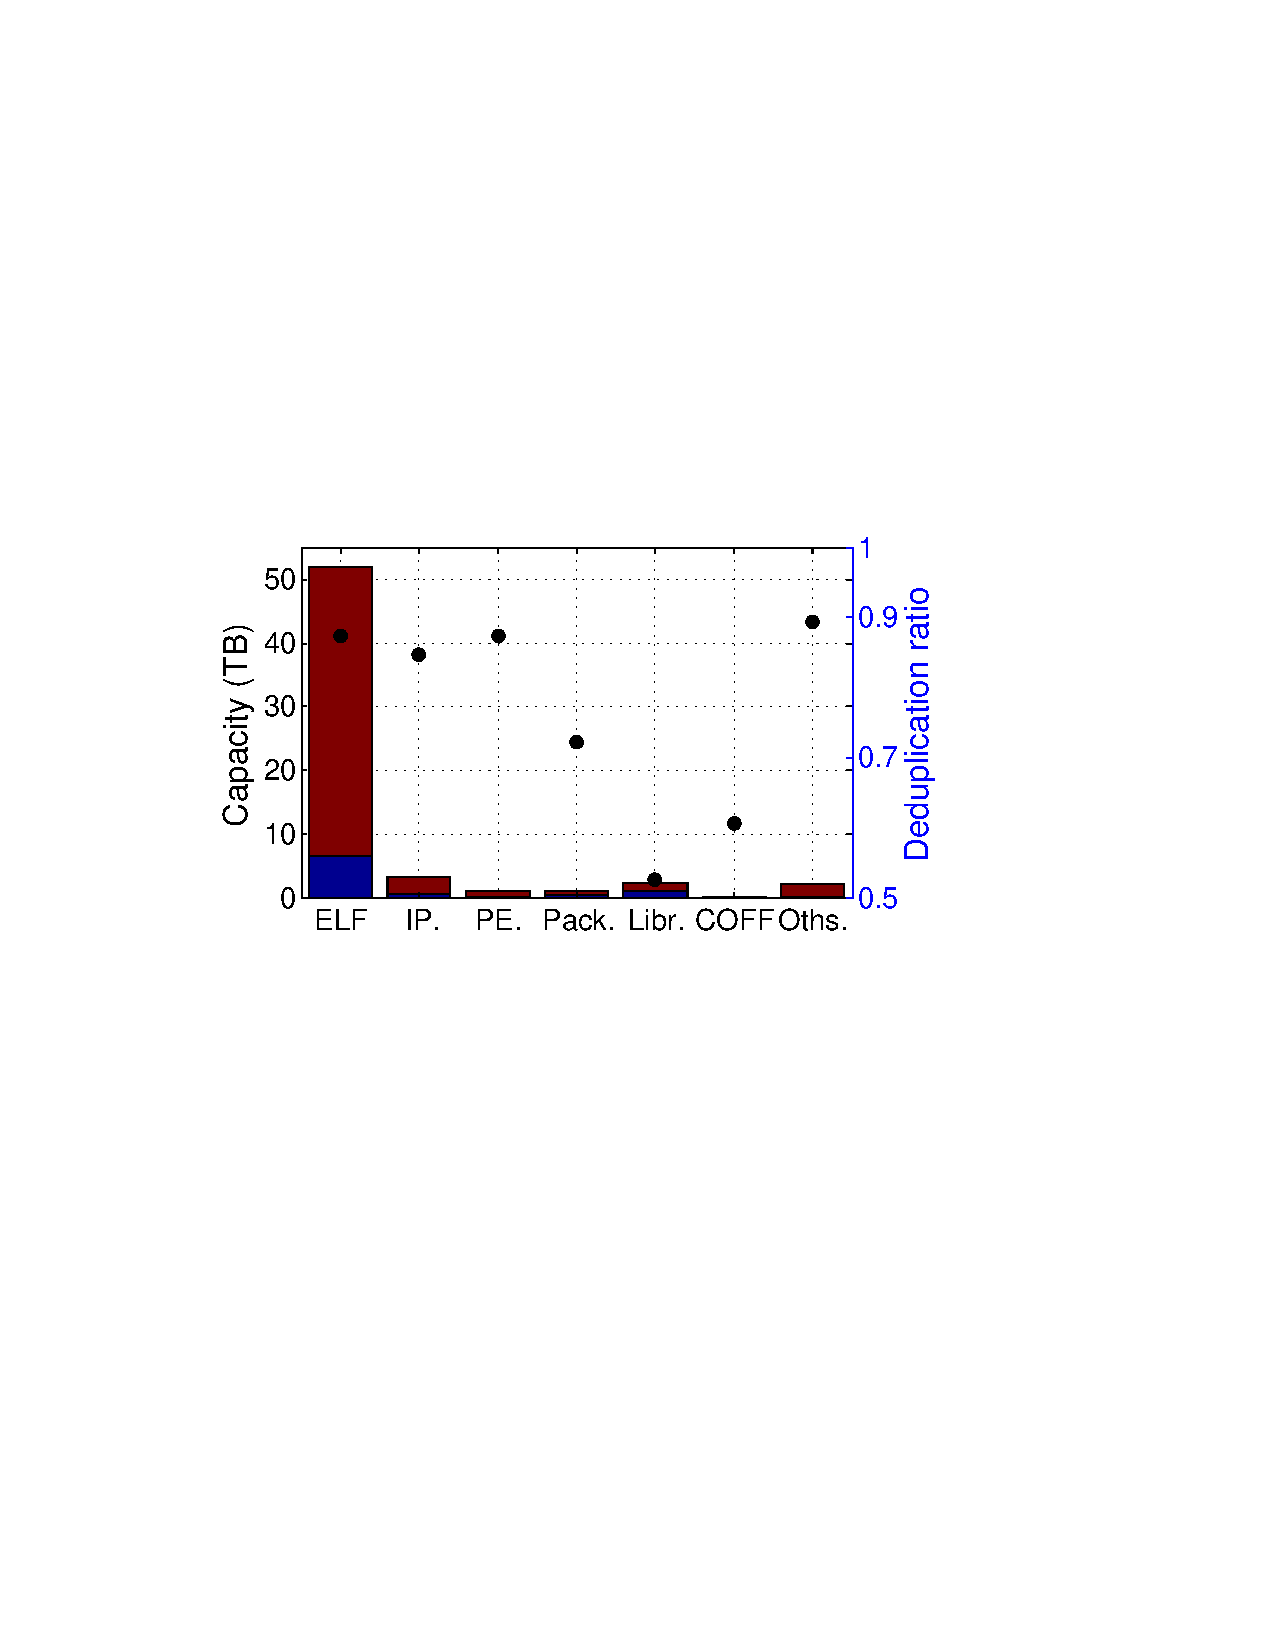
\includegraphics[width=0.35\textwidth]{graphs/dedup-eol} 
%	\caption{Deduplication results for EOL files: ELF, intermediate representation, PE32/PE32+ files, Debian/RPM binary packages, 	Libraries, COFF files.} 
%	\label{fig:dedup-eol}
%\end{figure}
%
%\paragraph{Executable, object code, and libraries (EOL)} We further calculated
%the deduplication ratio for specific file types in each common type group. 
%%
%We
%started from EOL group since it occupies the most capacity and contributes a
%lot to the overall savings after deduplication. 
%%
%Figure~\ref{fig:dedup-eol} shows the deduplication results for EOL files.  
%%
%We
%see that ELF files, intermediate representations, and PE files have the highest
%deduplication ratio (around 87\%). 
%%
%Especially, the redundant ELF files occupy
%the most capacity (73.4\%). 
%%\nancomment{replace MS exec with PE files}
%Libraries and COFF files have the lowest deduplication ratio of 53.5\% and 61\%
%respectively.
%
%We also calculated the deduplication ratio for each intermediate representation
%and libraries. 
%%
%We found that all the intermediate representations have a very
%higher deduplication ratio (greater than 77\%). 
%%
%Especially, the redundant
%Python byte-compiled codes take up to 67\% of capacity occupied by intermediate
%representations. 
%%
%Although overall library's deduplication is lower, we found
%that GUN C/C++ library and Palm OS dynamic library have a higher deduplication
%ratio over 90\%.
%
%\textit{Finding 4: ELF files have the highest deduplication ratio among all EOL
%files and contribute most to the overall savings. Python byte-compiled codes
%have the highest deduplication ratio and also achieve a better capacity savings
%after dedupliation compared with other intermediate representations. Most
%libraries have the lowest deduplication ratio among all EOL files.}
%%
%%%As shown in , intermediate compiled files have the largest number of
%%redundant copies (333,261,220, 63.7\%), which only take up to 5.3\% (2.8TB) of
%%EOL redundant storage space, indicating that users creates more small
%%redundant intermediate compiled files. Among all the intermediate compiled
%%files, python byte-compiled files have the largest number of redundant copies
%%(64.1\%, 213,753,591), which account for 79.4\% (2.2TB) of EOL redundant
%%storage space as shown in Figure~\ref{fig:type-compiled}.  % %We found that
%%there are various redundant intermediate compiled files in layers in addition
%%to Python byte-compiled, such as Erlang beam files, Xemacs/emacs compiled
%%files, compiled Java class, Mach-o fat files, Guile object bytecode, and llvm
%%bitcode files. We see that 21.6\% (71,830,155) and 10.12\% (33,740,399) of
%%redundant intermediate compiled files are terminfo compiled and compiled java
%%class files, which consume 76.4 GB and 104.4 GB storage space.   
%%
%%%ELF files have the largest redundant capacity %A large executable group is
%%ELF file type, which consists of ELF 64/32-bit LSB relocatable, shared object,
%%executable, core file, processor-specific for x86-64, MIPS, %ARM, Intel 80386,
%%etc. architectures.  %Another executable group contains VAX COFF executable,
%%PE32/PE32+ executable for Windows, and 386 pure executable, VMS Alpha, etc.
%%%\% of files are script executable, which contains python, shell, etc.  %\% of
%%files are RPM, Debian bin
%%
%%%\begin{figure} %	\centering %
%%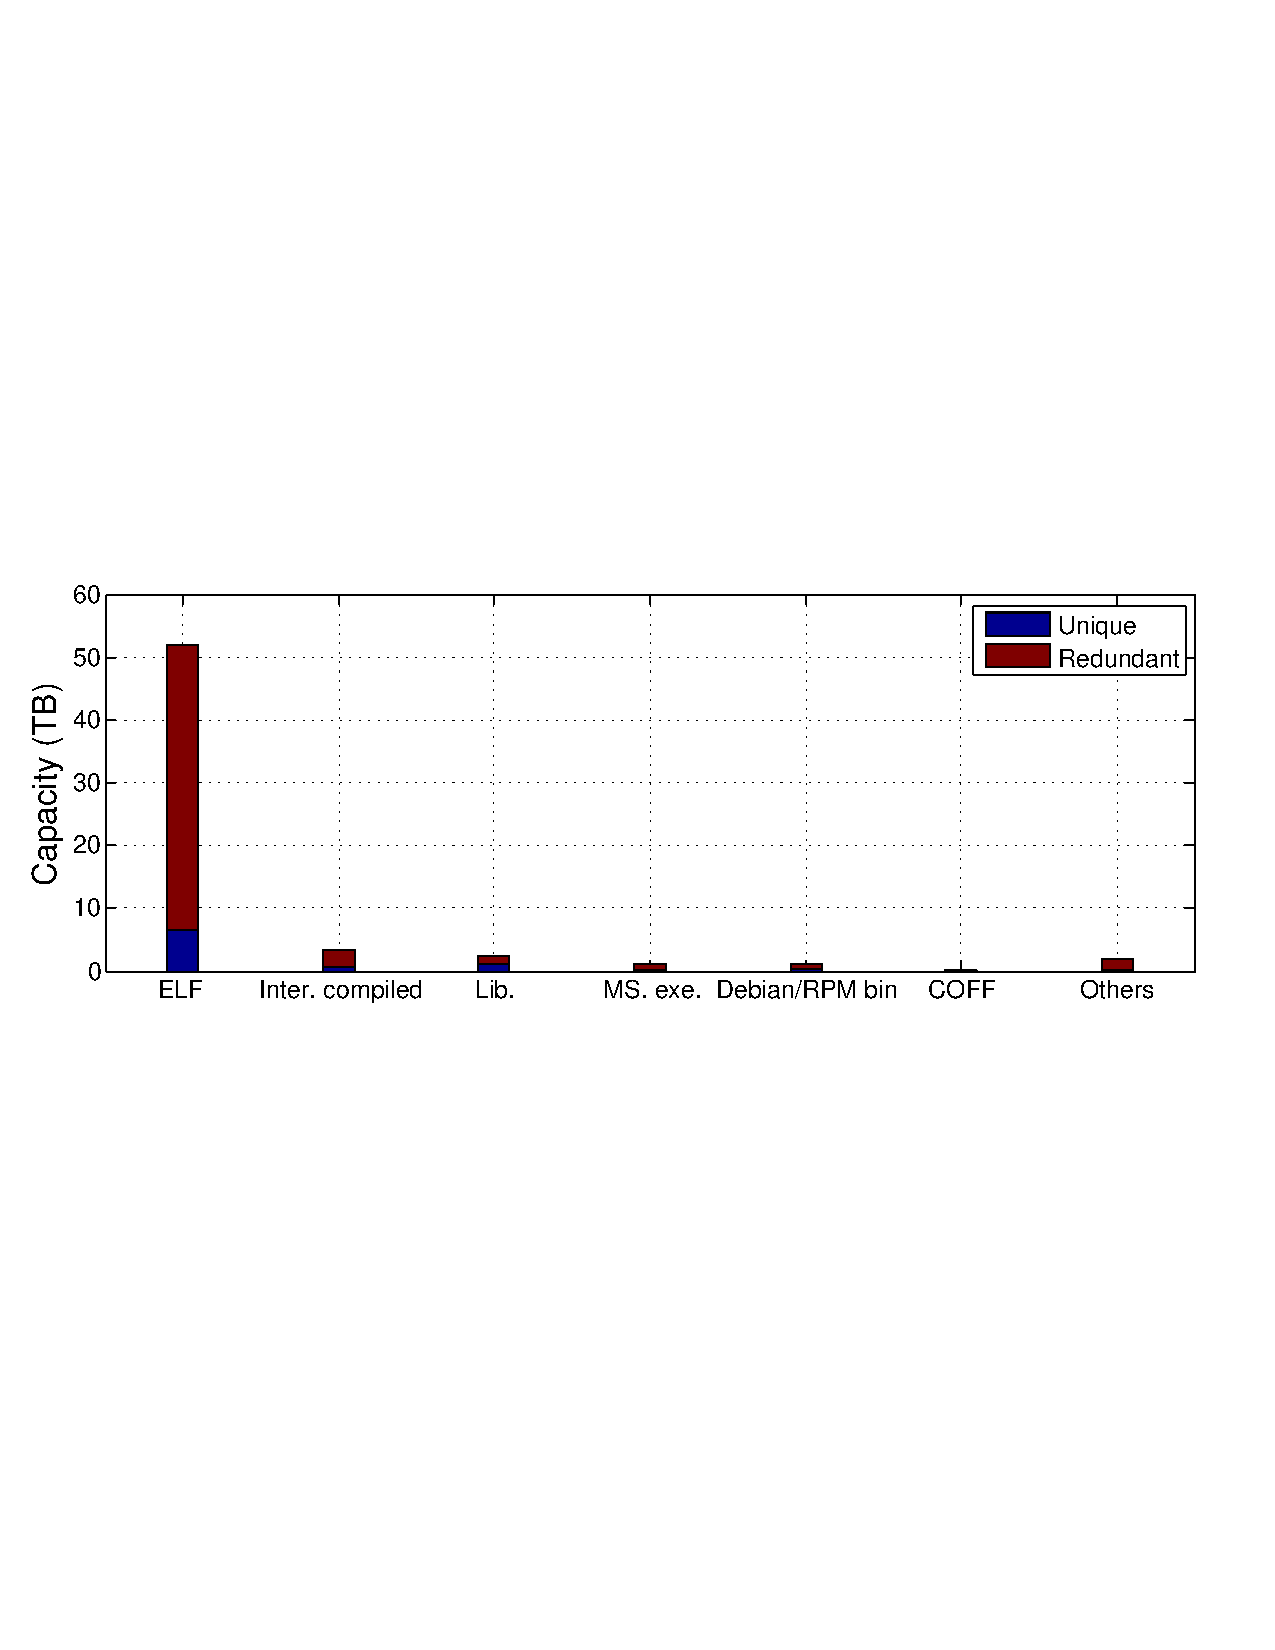
\includegraphics[width=0.5\textwidth]{graphs/type-exec-cap} %
%%\caption{\nancomment{Deduplication results for EOL files}.  %	} %
%%\label{fig:type-eol} %\end{figure}
%%
%%%Finding 2: 31.4\% (164,059,690) and 63.7\% (333,261,220) of EOL files are ELF
%%files and intermediate compiled files, which take up over 85.7\% (45.3TB) and
%%5.3\% (2.8TB) of redundant storage capacity, indicating that users replicate
%%or create more identical ELF files and intermediate compiled files. 64.1\%
%%(213,753,591) of intermediate compiled files are Python byte-compiled files,
%%which take up to 79.4\% (2.2TB) of redundant storage space, indicating that
%%users compiled more Python scripts (similar to Finding 2.)
%%
%\paragraph{Source code (SC.)}
%%
%%%Finding 3: 80.2\% (548,507,865) of source codes are C/C++ source, which take
%%up to 79.7\% (4.2TB) of redundant storage space, indicating that users are
%%more prone to duplicate C/C++ codes, which results in more ELF file replicas.
%%%The last group contains
%%
%\begin{figure} 
%	\centering
%	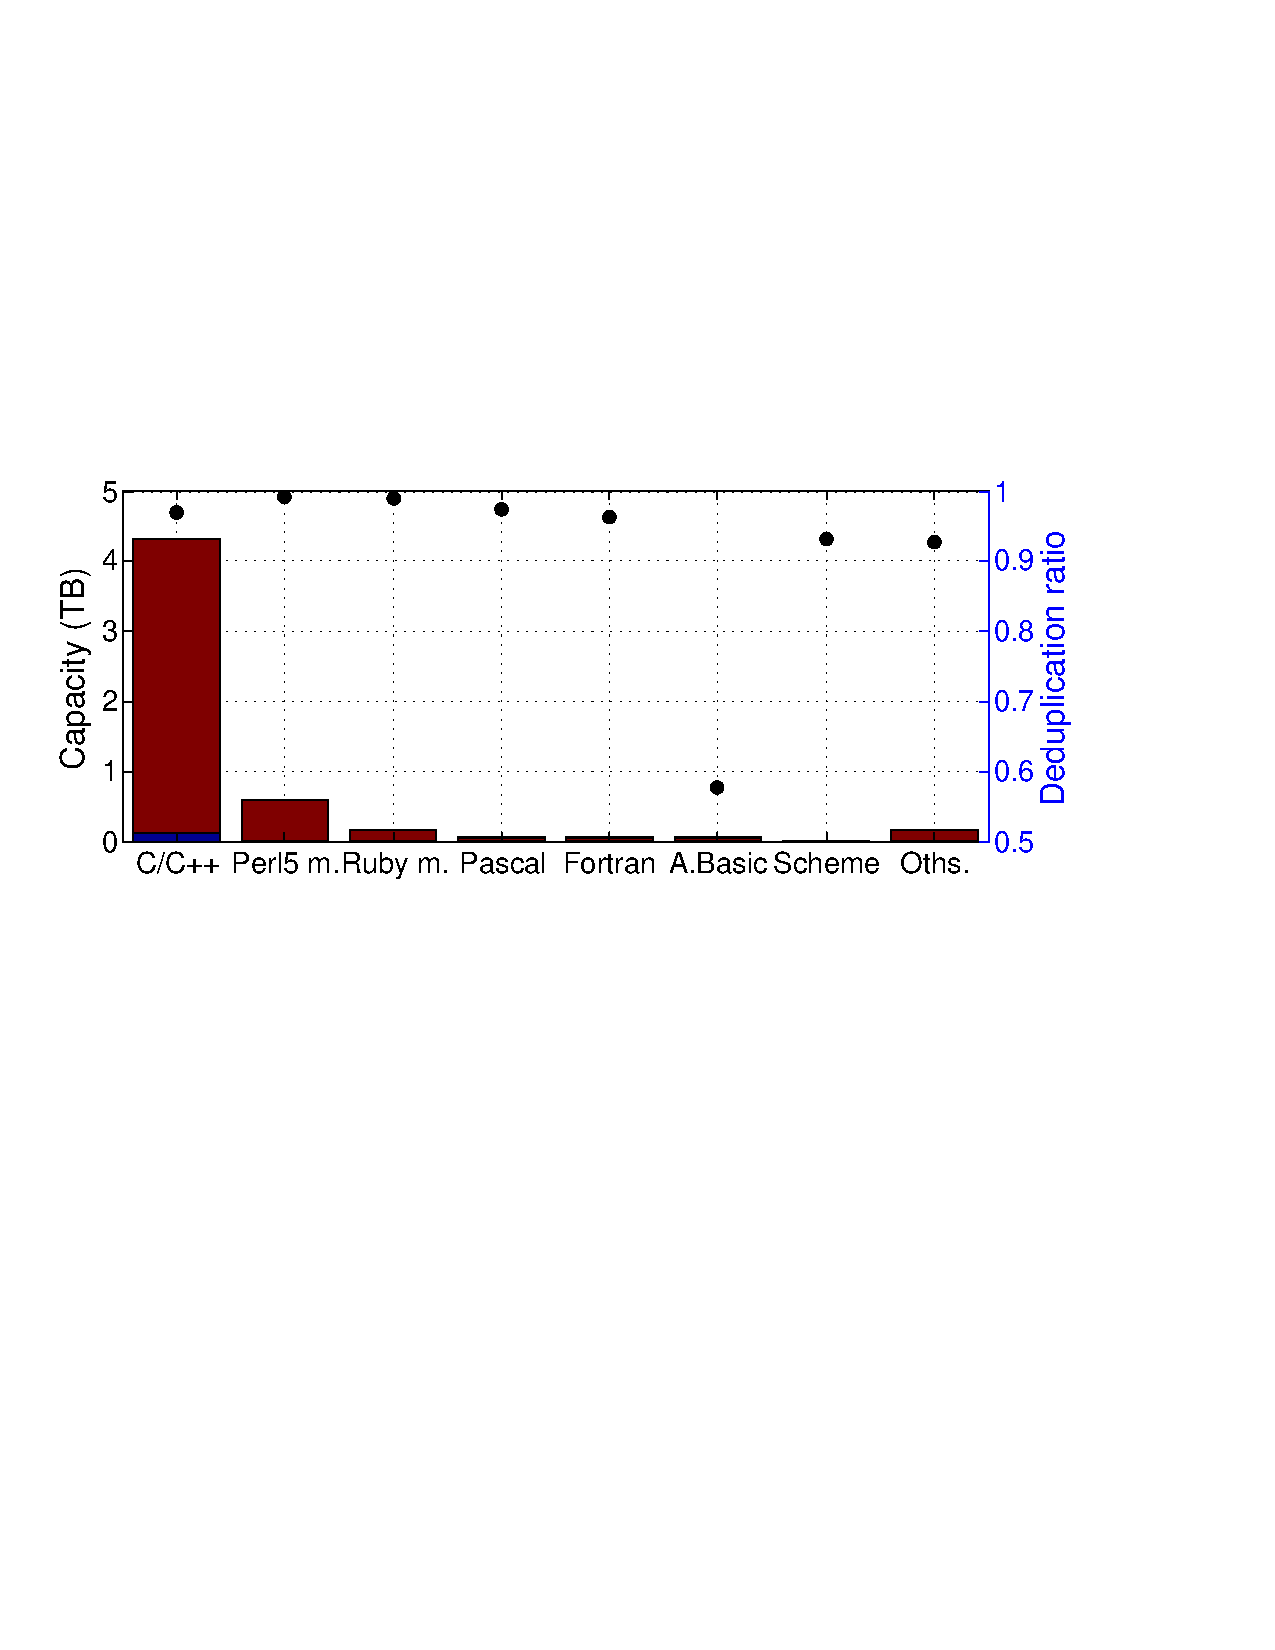
\includegraphics[width=0.35\textwidth]{graphs/dedup-sc} 
%	\caption{Deduplication results for source codes: C/C++ source, Perl5 module source, ruby module
%		source, pascal program, fortran program, Applesoft Basic program, Lisp/scheme
%		program, and other source codes.  } 
%	\label{fig:dedup-sc} 
%\end{figure}
%
%As discussed, Docker developers are more prone to replicate codes. 
%%
%To find out
%which kind of source codes are replicated frequently, we conducted
%deduplication on 7 common source codes as shown in Figure~\ref{fig:dedup-sc}.
%
%We see that all the source codes have a high deduplication ratio over 90\%
%except Lisp/scheme program. 
%%
%Especially, the redundant C/C++ source codes take
%up over 77\% of capacity occupied by source codes. 
%%
%To find out why there are so
%many C/C++ source codes, we inspect the C/C++ source codes and find a
%frequently replicated C/C++ source code called Google Test~\cite{googletest}, which is
%a cross-platform C++ test framework and available in GitHub~\cite{github}.
%%
%Interestingly, we found there are plenty of repositories related to Google Test
%while there is no official repository for Google Test. 
%%
%We suspect that many
%developers replicate open source code from external public repositories, such
%as GitHub, and store them in containers. 
%%
%This would also explain why there are
%so many shared source codes across different images. 
%%
%Docker Hub
%allows developer to automatically build images from source code in external
%public repositories and automatically push the built image to their Docker
%repositories. Thus we believe that more open source code would be replicated into
%different images stored in Docker Hub registry. 
%%
%\textit{To eliminate redundant
%open source codes in Docker registry in the future, we suggest that Docker Hub
%can create more offical images for popular open source codes so that developers
%can directly pull the image as a read-only layer. }
%
%\textit{Finding 5: C/C++ source codes have a high redundant ratio and
%contribute a lot to the overall savings. Many redundant source codes shared
%cross images are replicated or automatically build from external public
%repositories. To eliminate redundant source codes in Docker registry, we
%suggest to create more official images for these open source codes and convince
%developers to pull them from registry.}
%%
%%%\nancomment{found some libc++ source code here, did not put them into
%%libraries.} % shows the redundant file count and storage capacity distribution
%%for source code. C/C++ source codes have the largest number of redundant
%%files. 80.2\% (548,507,865) of source codes are C/C++ source, which take up to
%%79.7\% (4.2TB) of redundant storage space, indicating that users are more
%%prone to duplicate C/C++ codes, which results in more ELF file replicas.
%%
%%%We also found other source codes, such as Perl5 module source code (9.5\%),
%%ruby module source code (7.6\%), assembler source code (1.1\%), pascal source
%%(0.7\%), fortran program code (0.01\%), applesoft basic source code, and
%%Lisp/scheme source code (0.17\%).
%%
%%%\begin{figure} %	\centering %
%%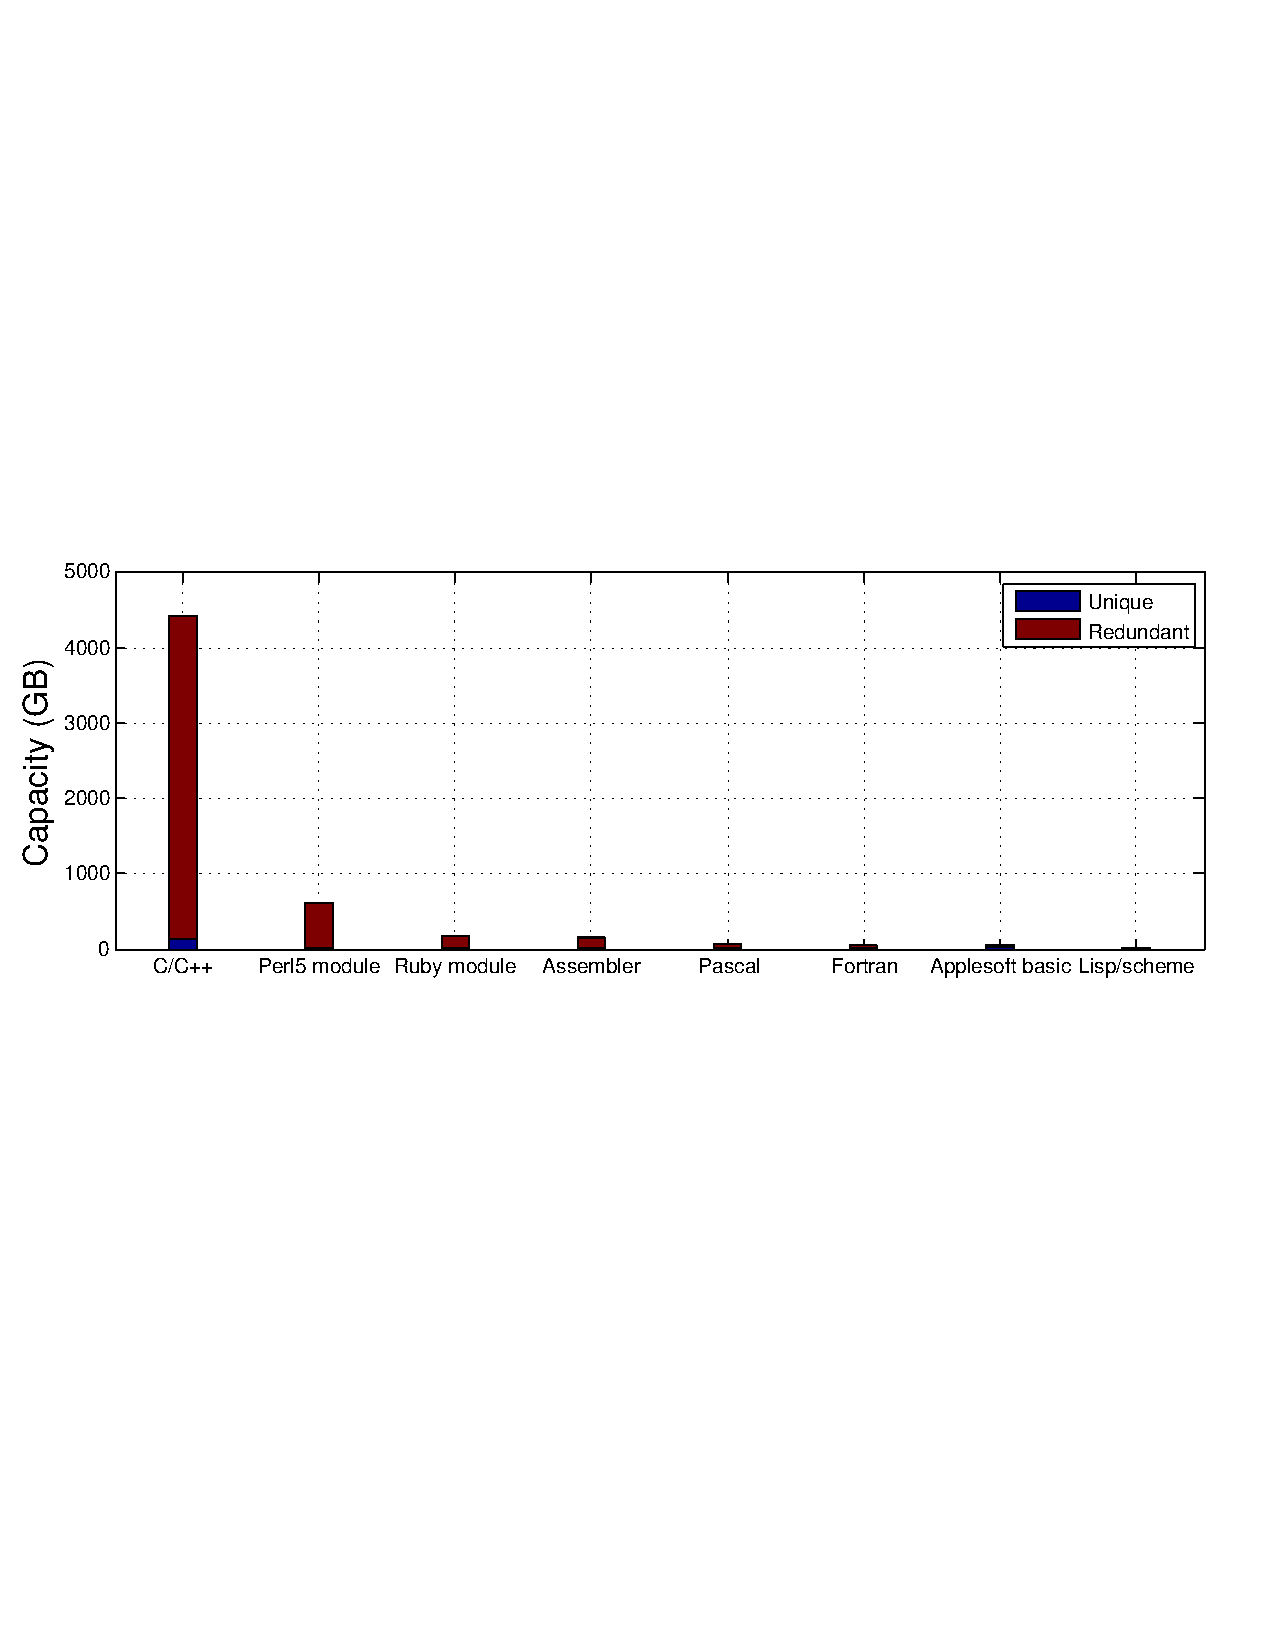
\includegraphics[width=0.5\textwidth]{graphs/type-lang-cap} %
%%\caption{Redundant data vs. unique data for source code files.  %	} %
%%\label{fig:type-source} %\end{figure}
%%
%%%Figure~\ref{fig:type-lib} shows the redundant library distribution. We see
%%that Gcc precompiled header files have the lowest number of redundant library
%%files (20.3\%), but they take up to 0.93 TB. Almost 86.4\% of redundant
%%library files are Palm libraries, which only take up to 7.2GB space,
%%indicating that gcc compiled header files are much bigger than other
%%libraries.  % %We also found there are different libraries used in layers,
%%such as netcdf library, Ocaml lib., mach-o lib.
%%
%%%Figure~\ref{fig-elf} %\subsection{Lib} % %library files contains libtool
%%library file, OCaml native library, MIT scheme, Mach-O library, OCaml library,
%%Palm OS dynamic library data, Microsoft c/c++ library.current ar archive
%%random library, and other library.
%%%%libtool\|OCaml\|Palm\|MIT\|microsoft\|current ar archive random
%%library\|mach-o\|rpm\|gzip %\subsection{Source code}
%%
%\paragraph{Scripts(Scr.)}
%%%Finding 2: 53.6\% (238,353,674) of redundant scripts are Python scripts,
%%which take up over 2.6TB storage space, indicating that users are more prone
%%to replicate Python scripts compare to other scripts.
%%
%%%\begin{figure} %	\centering %
%%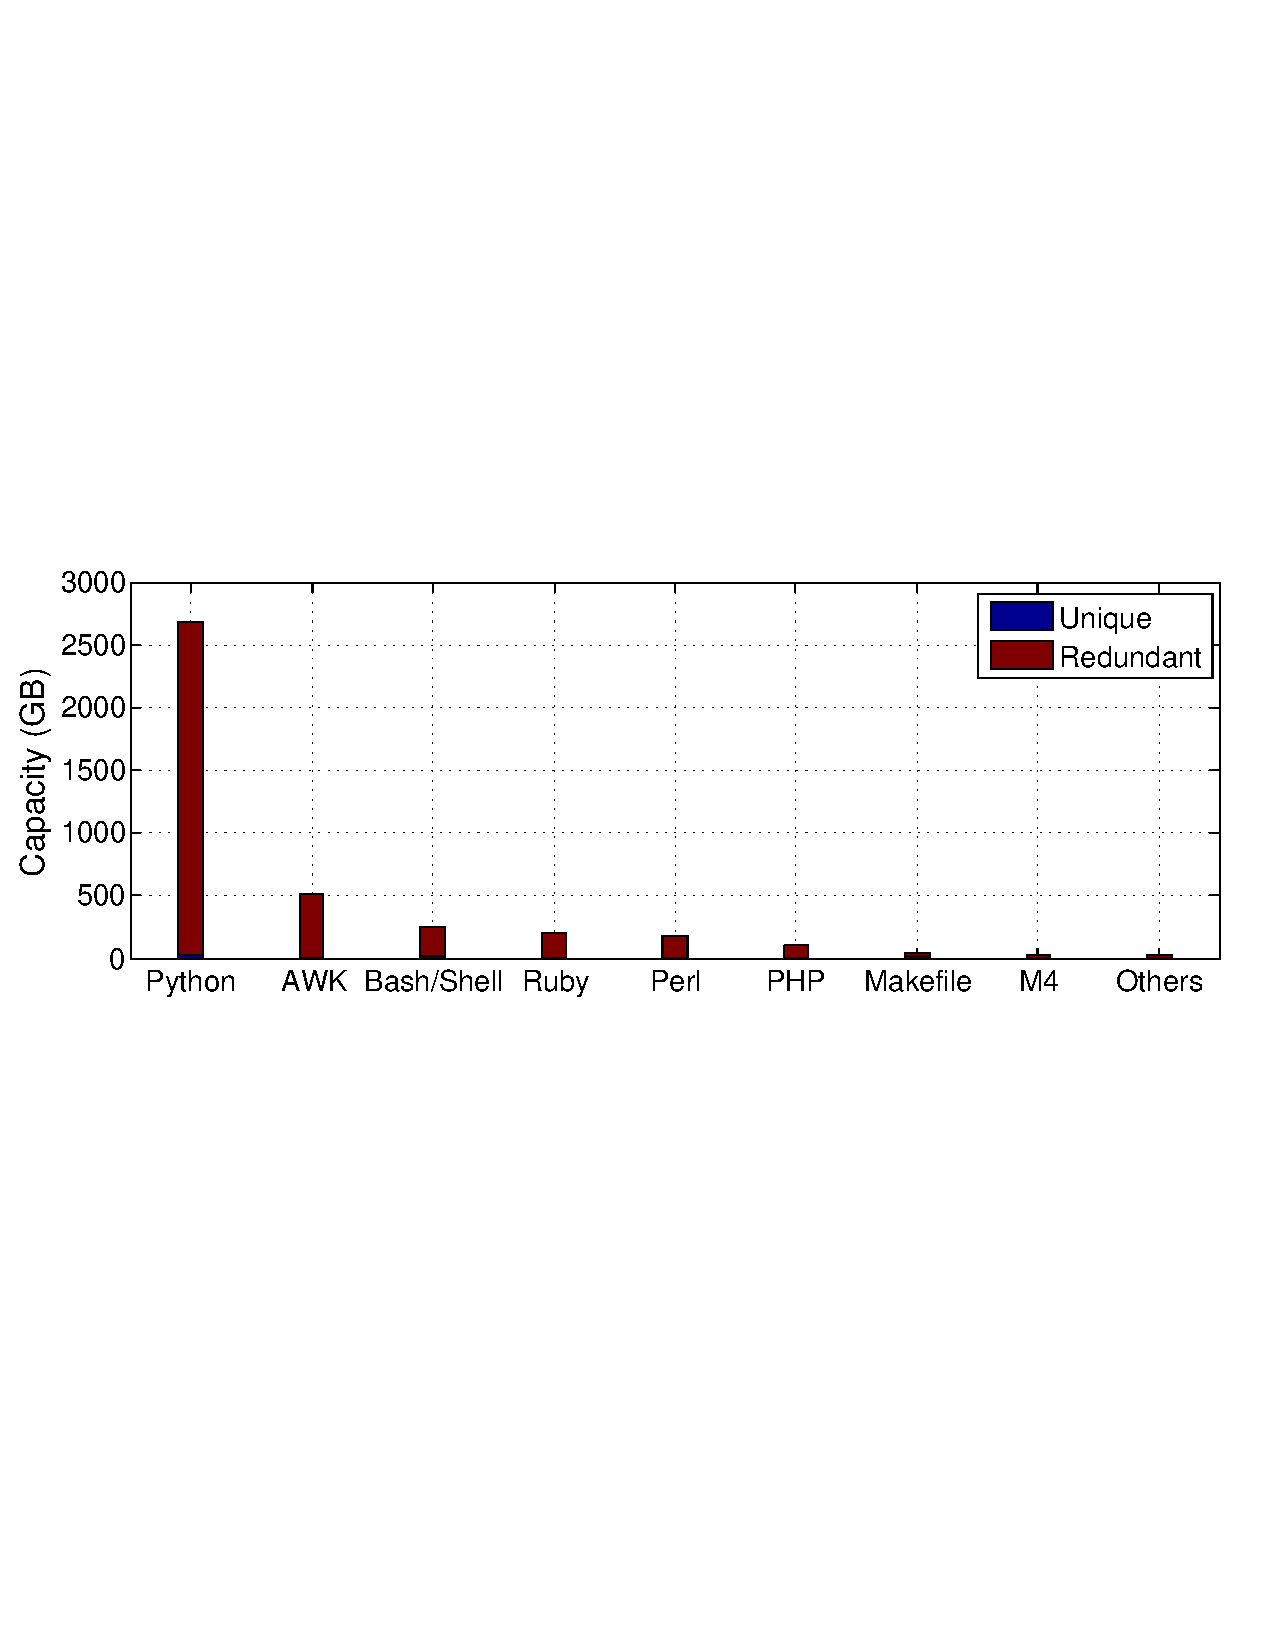
\includegraphics[width=0.5\textwidth]{graphs/type-script-cap} %
%%\caption{Redundant data vs. unique data for scripts.  %	} %
%%\label{fig:type-script} %\end{figure}
%%
%
%\begin{figure} 
%	\centering
%	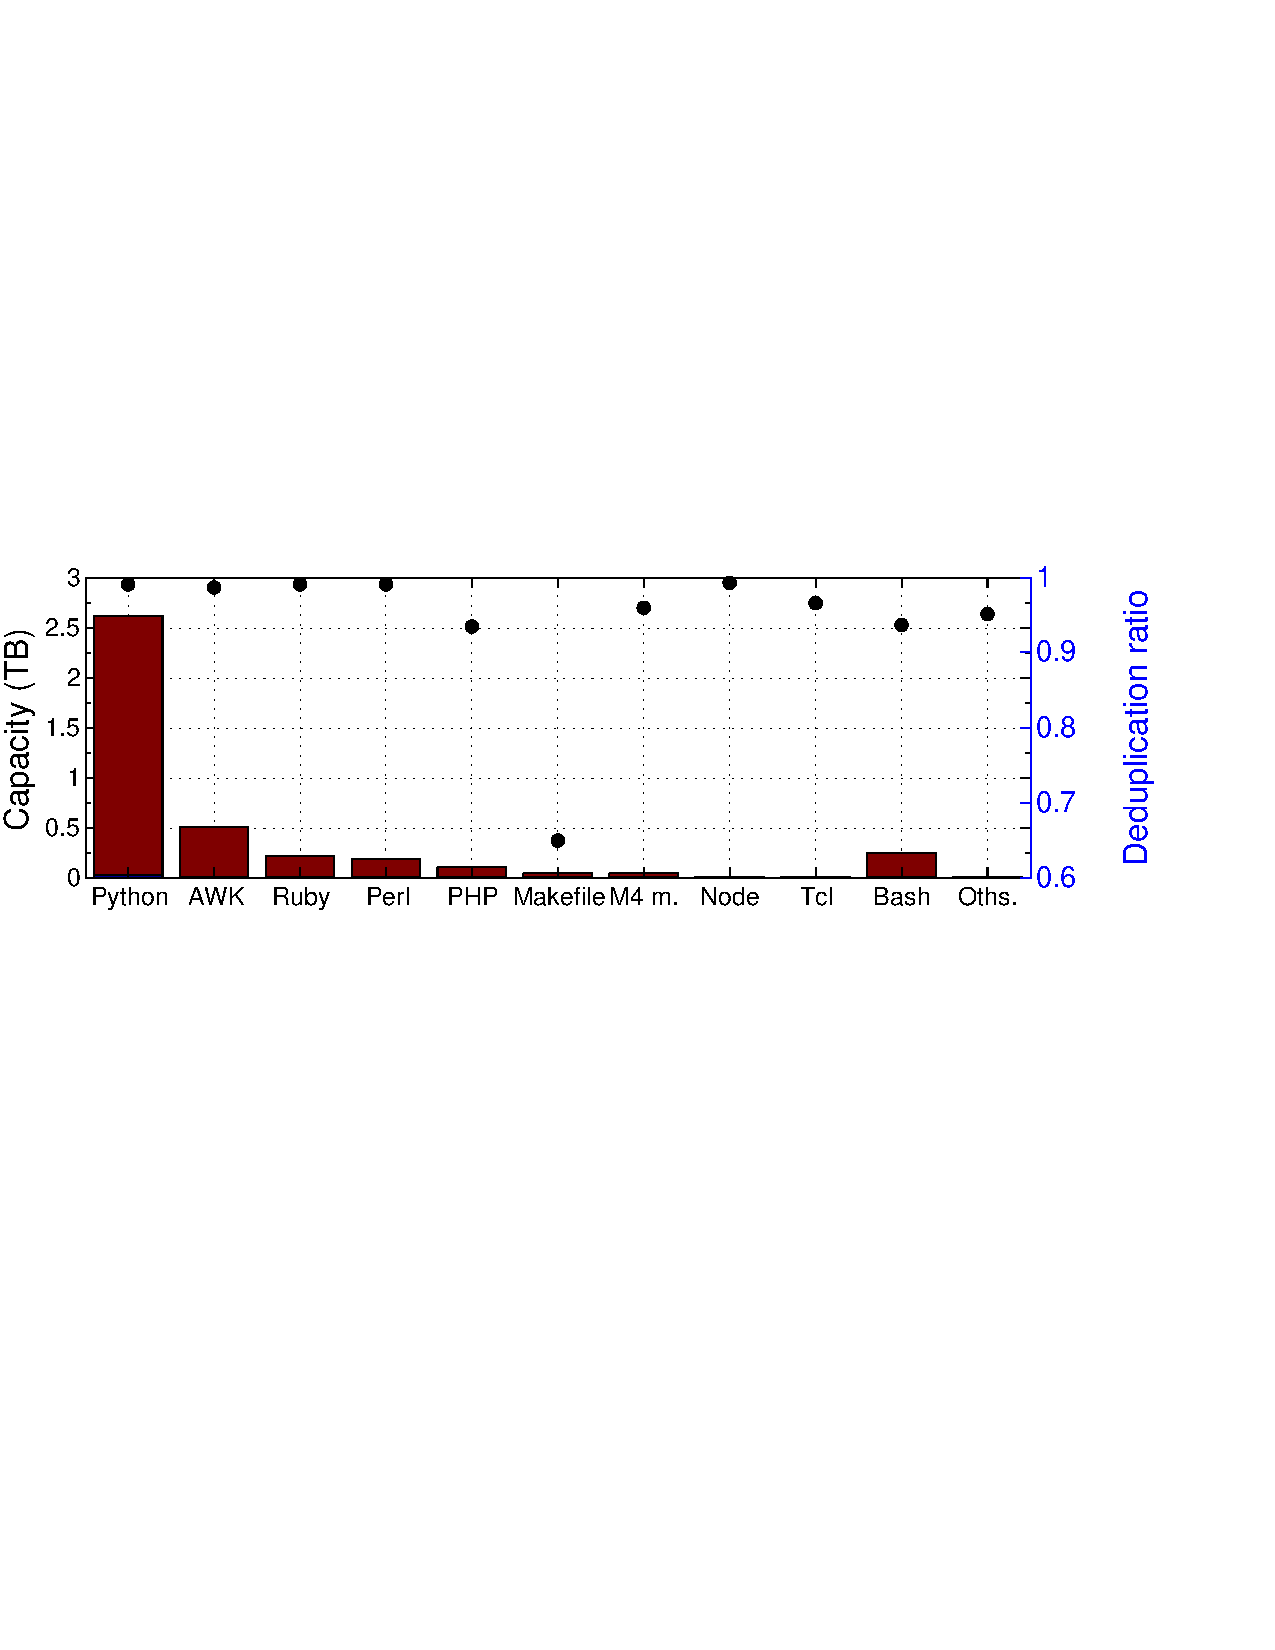
\includegraphics[width=0.45\textwidth]{graphs/dedup-scrp}
%	\caption{Deduplication results for scripts: python, AWK, ruby, perl, PHP, makefile, M4 macro processor, node, Tcl, bash and other scripts.}
%	\label{fig:dedup-scrp} 
%\end{figure}
%
%Similar to source codes, we present the deduplication ratio for scripts as
%shown in Figure~\ref{fig:dedup-scrp}.  
%%
%We see that most of the scripts have a
%high deduplication ratio over 95\%. 
%%
%Especially, the redundant Python scripts
%take up over 65\% of capacity occupied by scripts. 
%
%We inspect the Python scripts and found a frequently replicated Python scripts
%called kraken-tools~\cite{krakentools}, which is a tool for managing system
%requirements for kraken-lib~\cite{krakenlib}. 
%%
%kraken-lib is an orchestration and
%cluster-level management system for Kubernetes~\cite{kubernetes}.
%%% a tool for  for Kubernetes cluster.  %kraken-lib %Kubernetes is an open
%%source platform that automates Linux container operations 
%%
%Although kraken-tools seems like an Docker image repository, it is maintained
%in GitHub rather than Docker registry. 
%%
%Interestingly, kraken-lib does not have
%a official repository in Docker Hub but it has a public repository in QUAY
%registry~\cite{quay}.  
%%
%\textit{Similar to source codes, we suggest to create
%more official images in registry for some popular public scripts %, especially
%containerized applications and convince developers to pull them from registry
%as a read-only layer to reduce redundant scripts in registry.}
%
%\textit{Finding 6: Scripts have a very high deduplication ratio. Especially,
%redundant Python scripts contribute a lot to the overall savings. Many
%redundant scripts are replicated from external public repositories such as
%GitHub.  we suggest to create more official images for these public scripts and
%convince developers to pull them from registry.}
%%% shows the redundant scripts distribution. Python script has the largest
%%number of redundant scripts (238353674, 53.6\%), which take up to 2.6TB
%%storage space, indicating that users are more prone to replicate Python
%%scripts compare to other scripts.  %%This finding also explains that why
%%python byte compiled files takes the largest proportion of intermediate % %We
%%find that users use different scripts in the images.  %For example, 20\%,
%%9.7\% and 4.4\% of scripts are bash/shell scripts, ruby scripts, and awk
%%scripts. Other scripts such as perl script (4.2\%), php script(3.9\%),
%%makefile script(1.3\%), and M4 macro processor script(0.7\%) are also used.
%%
%\paragraph{Documents(Doc.)}
%%%Finding 3: 79.7\%, 5.2\%, and 12.4\% of redundant documents are ASCII text,
%%UTF-8/16 text, and HTML/XML/XHTML, which take up over 11TB, 3.4TB, and 3.9TB
%%redundant storage, indicating that users replicate more ASCII text, UTF-8/16
%%text, and HTML/XML/XHTML compare to other documents.
%%
%\begin{figure} 
%	\centering
%	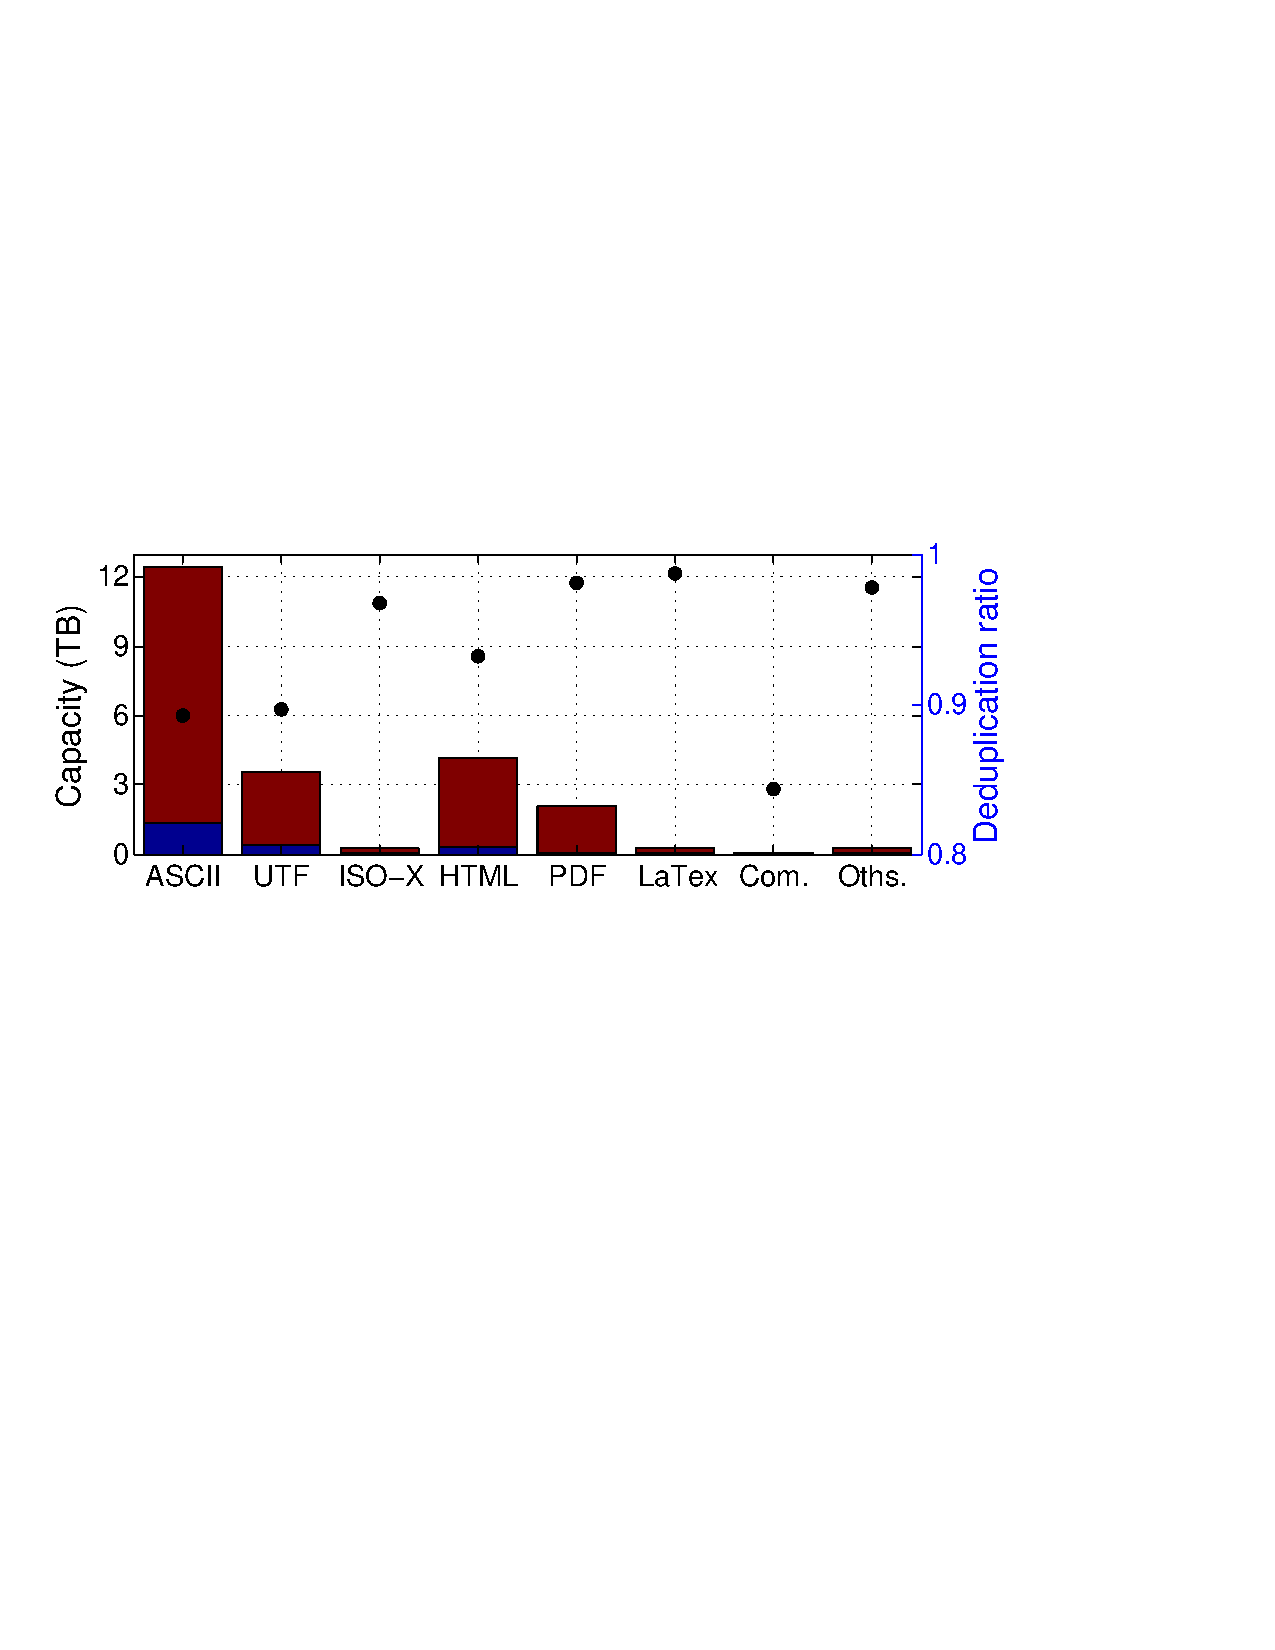
\includegraphics[width=0.35\textwidth]{graphs/dedup-doc} \caption{Deduplication
%	results for documents: ASCII, UTF, ISO-8859, HTML/XML/XHTML, PDF, LaTex
%	documents, Composite document files, and others.} 
%	\label{fig:dedup-doc}
%\end{figure}
%
%Next, we present the deduplication results for different documents as shown in
%Figure~\ref{fig:dedup-doc}.  
%%
%We see that all the documents have a very high
%deduplication ratio of 84\% or higher.  
%%
%Especially, redundant raw text files
%and HTML/XML/XHTML documents take up over 48\% and 17\% of capacity occupied by
%documents. 
%%
%To understand why there are so many document duplicates, we inspect
%raw text files and HTML/XML/XHTML documents respectively. 
%%
%First, we found that
%a large amount of redundant raw text files are input data for testing source
%codes and they are replicated along with source code or script projects from
%external public repositories.  
%%
%For example, scipy~\cite{scipy}, a
%metamathematical software, is replicated from GitHub and stored in different
%images, which contains over 30 raw text files for testing purpose.
%
%Second, after inspected HTML/XML/XHTML documents, we found plenty
%HTML/XML/XHTML documents serves as readme, manual, or license. 
%%
%For example, we
%found plenty redundant HTML documents related to gnome-vfs-doc~\cite{gnome-vfs-doc},
%which are documentation for GNOME virtual filesystem subsystem available
%online~\cite{gvfs}.
%
%\textit{Finding 7: Documents have a very high redundant ratio. Majority
%redundant documents are raw text files and HTML/XML/XHTML documents. They are
%replicated along with source code or script projects and serves as input data
%for testing or informative documents.}
%%
%%%\begin{figure} %	\centering %
%%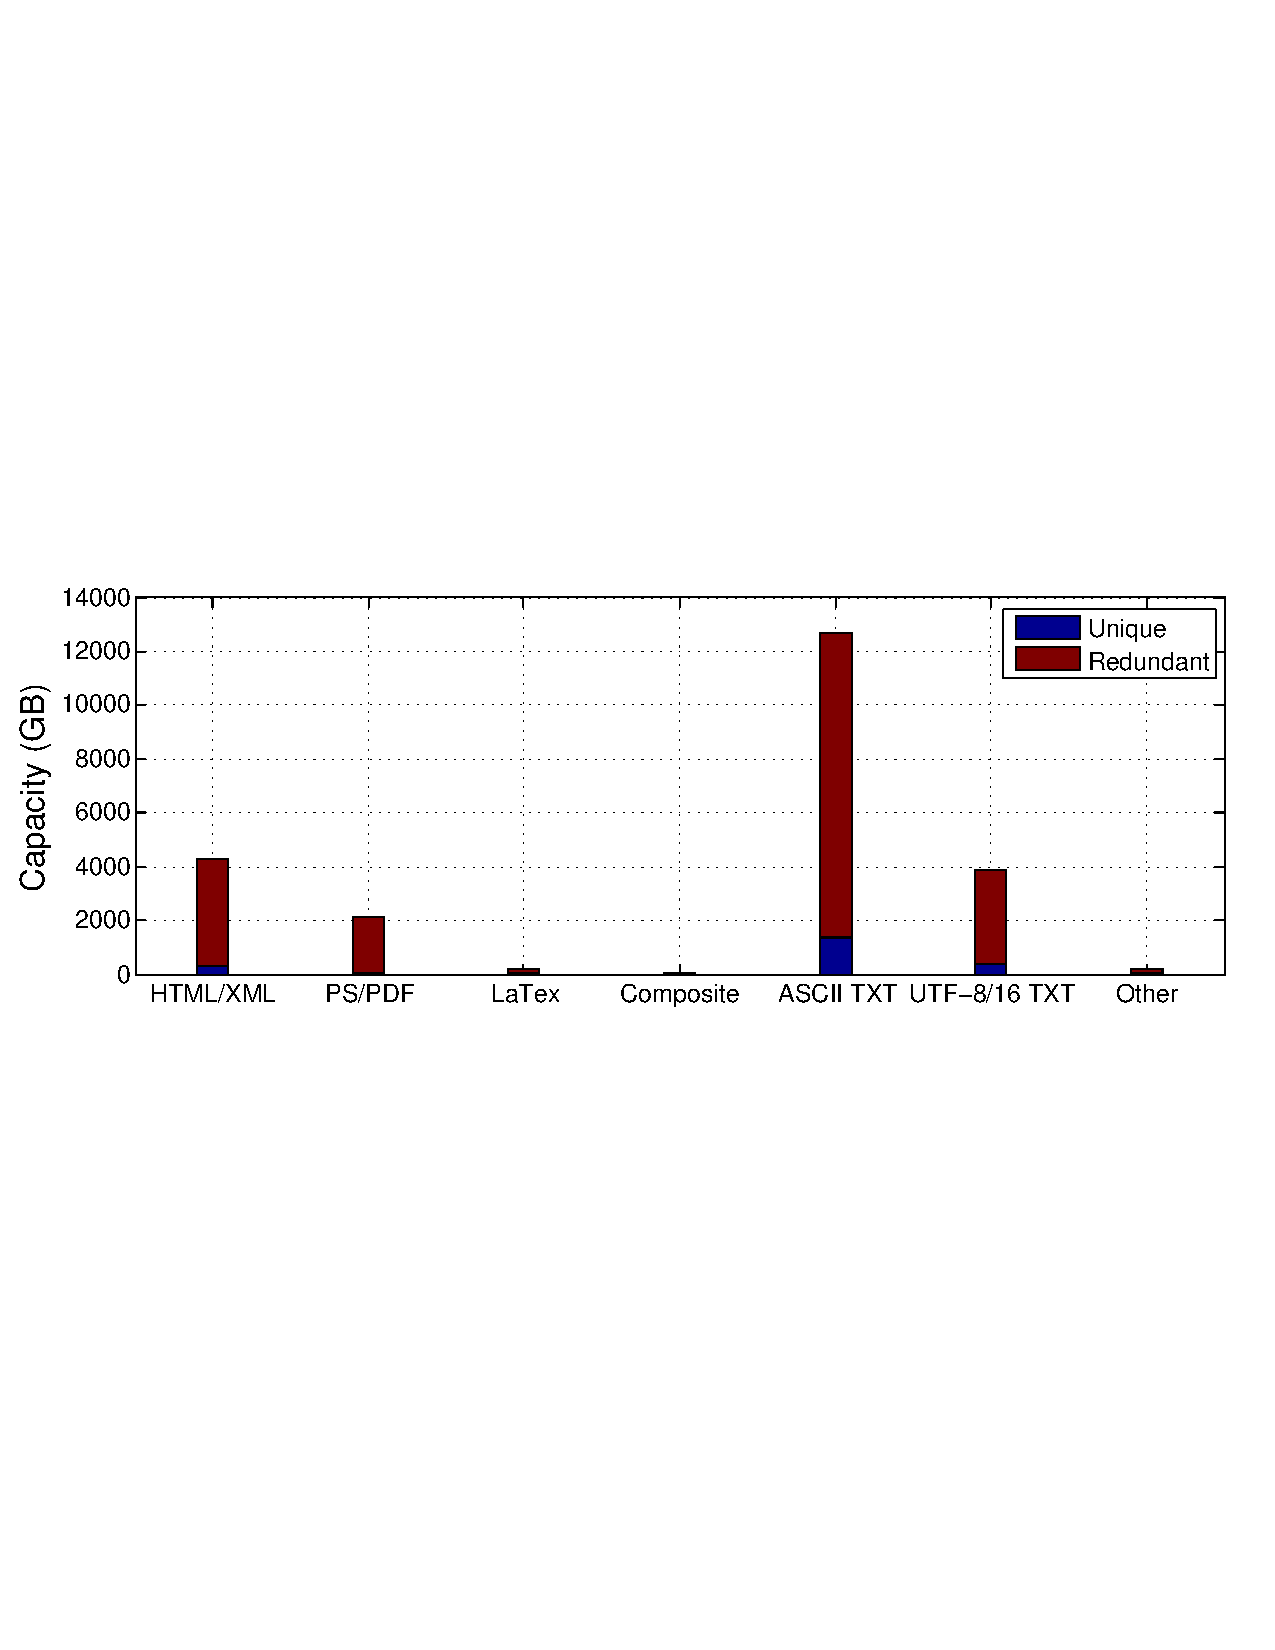
\includegraphics[width=0.5\textwidth]{graphs/type-utili-cap} %
%%\caption{Redundant data vs. unique data for documents.  %	} %
%%\label{fig:type-doc} %\end{figure}
%%
%%%https://pkgs.alpinelinux.org/contents?branch=edge&name=gnome-vfs-doc&arch=x86_64&repo=main
%%% presents redundant document distribution. We first group documents into two
%%categories: non-text documents and raw text documents.  %We see that ASCII
%%text files have the largest number of redundant document files (1,758,299,693,
%%79.7\%), which take up to 11TB storage space, indicating that users replicate
%%more ASCII text.  %12.4\% of the redundant documents are HTML/XML/XHTML
%%documents, which take up to 3.9 TB storage space, indicating users also
%%replicate HTML/XML/XHTML documents in images.  % %In addition to ASCII text,
%%5.2\% of redundant documents are UTF-8/16 unicode text, which take up 3.4 TB
%%storage space.  %Various documents are replicated in images, such as PS/PDF
%%documents (0.9\%), LaTex files (1.1\%) and Composite documents (0.01\%)
%%
%%%79.7\%, 5.2\%, and 12.4\% of redundant documents are ASCII text, UTF-8/16
%%text, and HTML/XML/XHTML, which take up over 11TB, 3.4TB, and 3.9TB redundant
%%storage, indicating that users replicate more ASCII text, UTF-8/16 text, and
%%HTML/XML/XHTML compare to other documents.  %type-utili-cap %type-script-cap
%%
%\paragraph{Databases (DB.)}
%%
%\begin{figure} 
%	\centering
%	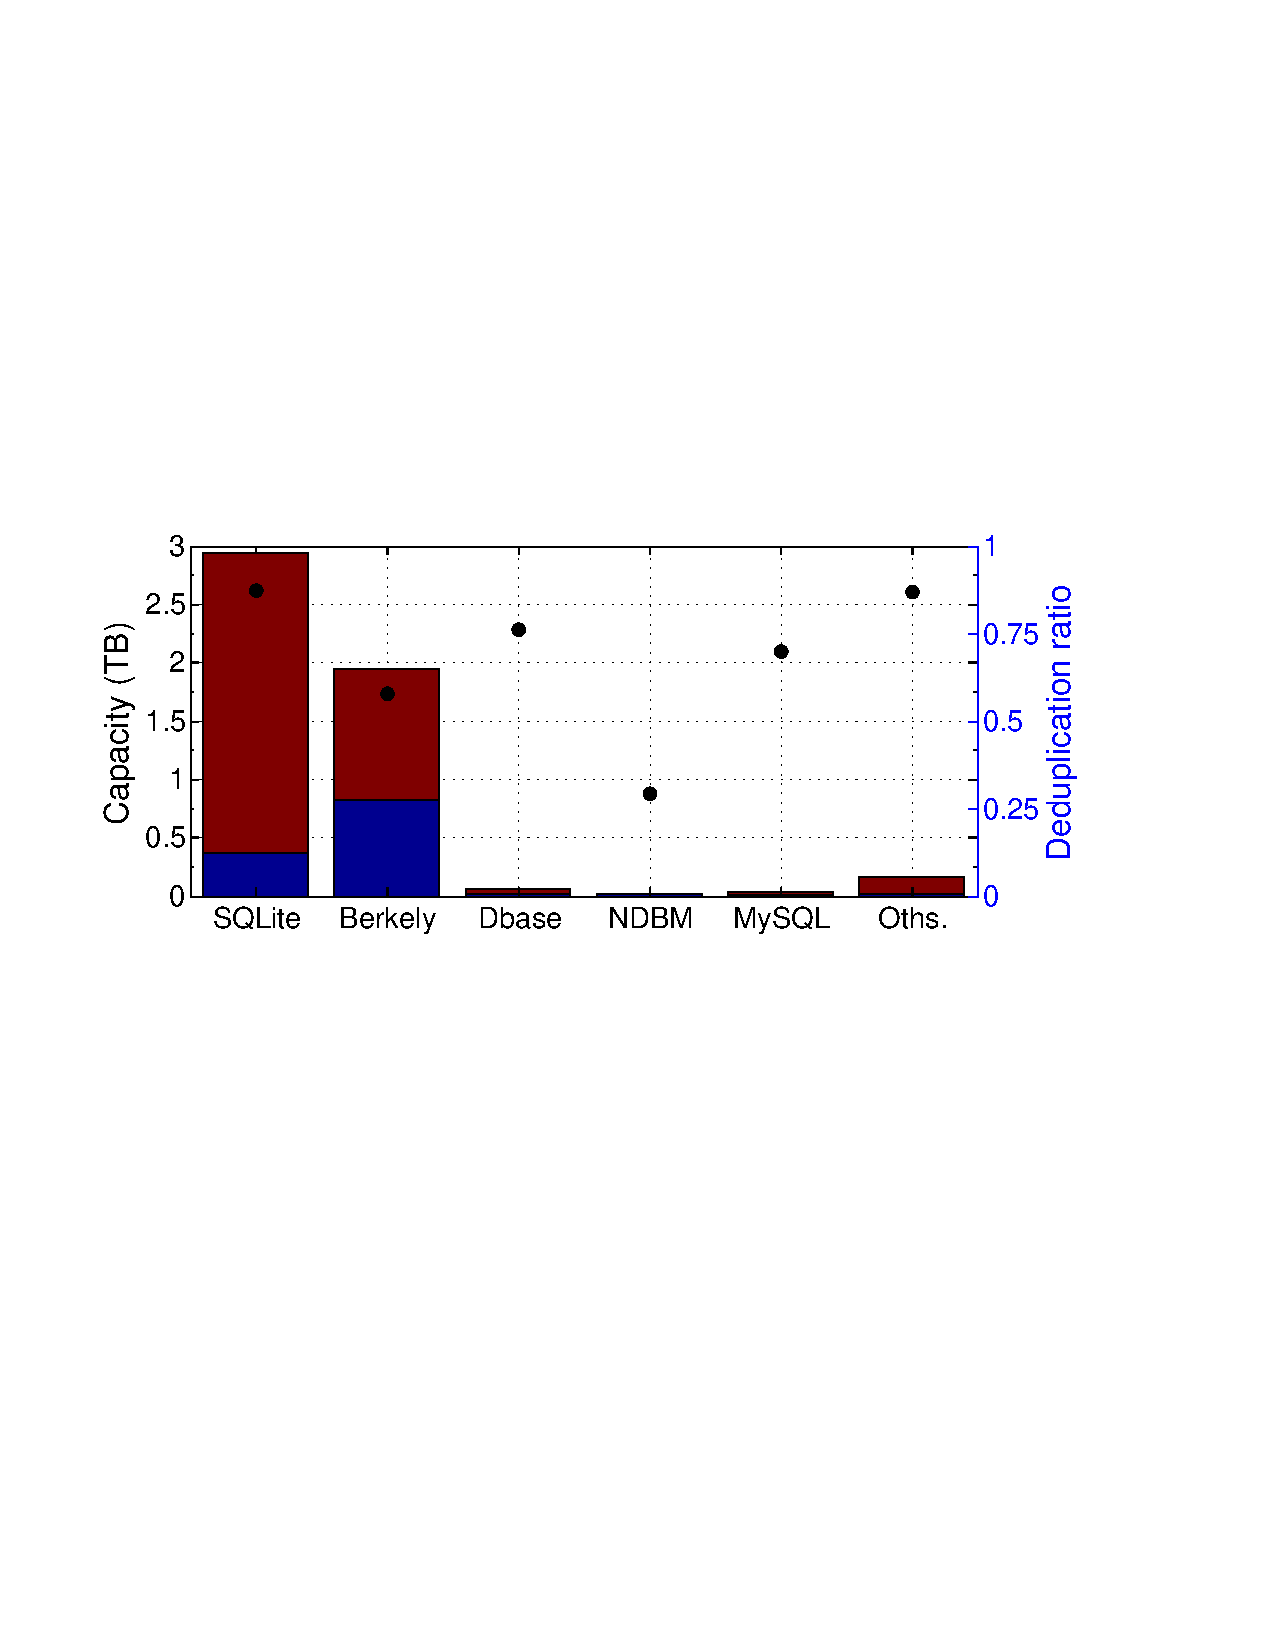
\includegraphics[width=0.4\textwidth]{graphs/dedup-db} \caption{Deduplication
%	results for database related files.  } 
%	\label{fig:dedup-db} 
%\end{figure}
%
%As discussed, Database related files have the lowest deduplication ratio at
%file-level. 
%%
%It makes sense because it's unusual for different users to create
%large amount of identical database files. 
%%
%Figure~\ref{fig:dedup-db} shows the
%deduplication ratio for different types of databases. 
%%
%We see that SQLite
%database files have the largest deduplication ratio of 87\% and could be
%deduplicated for saving up to half of the capacity. 
%%
%To find out why there are
%so many redundant SQLite files, we inspected SQLite files manually and found
%majority of redundant SQLite files are created by Yum~\cite{yum} for
%maintaining a list of well-know repositories.
%
%\textit{Finding 8: Databases have a low deduplication ratio. But SQLite files
%have the largest amount of redundant files and contribute a lot for saving
%capacity. The redundant SQLite files are mainly for saving identical list of
%repositories.}
%%
%%%primary_db.sqlite
%%
%%%Finding 4: 28.7\%, 30.9\%, and 11.9\% of redundant database files are
%%Berkeley DB, Mysql, and Dbase related files, which only take up over 1.1 TB,
%%26 GB, and 47.2 GB redundant storage, indicating that users replicate a lot
%%small database files related to Mysql and Berkeley DB. While there are only
%%7.3\% of SQLite files, which take up over 2.6TB storage space, indicating
%%SQLite files are much bigger than others.  % %Figure~\ref{fig:type-db}
%%presents database related redundant files. 30.9\% of redundant database
%%related files are related to MySQL, which only take up to 26GB storage space
%%while SQLite database related redundant files which only take up 7.3\% of
%%redundant database related files consume 2.56 TB storage space, indicating
%%users replicate more MySQL related files and bigger SQLite database related
%%files. %MySQL related files contains mysql table definitation files, mysql
%%misam index files, and mysql misam compressed data.  %Moreover, we also find
%%different redundant database related files are replicated in Docker images.
%%For example, 28.7\%, 11.86\%, and 5.57\% of redundant database files are
%%Berkeley DB, Dbase, and NDBM related files, which take up over 1.1 TB, 47.2
%%GB, and 7.7 GB redundant storage, indicating that users replicate database
%%files, especially, SQLite and Berkeley DB.  %While there are only 7.3\% of
%%SQLite files, which take up over 2.6TB storage space, indicating SQLite files
%%are much bigger than others.
%%
%%
%%%\begin{figure*}[t] %	\centering %	\begin{minipage}{0.35\textwidth} %
%%\centering %
%%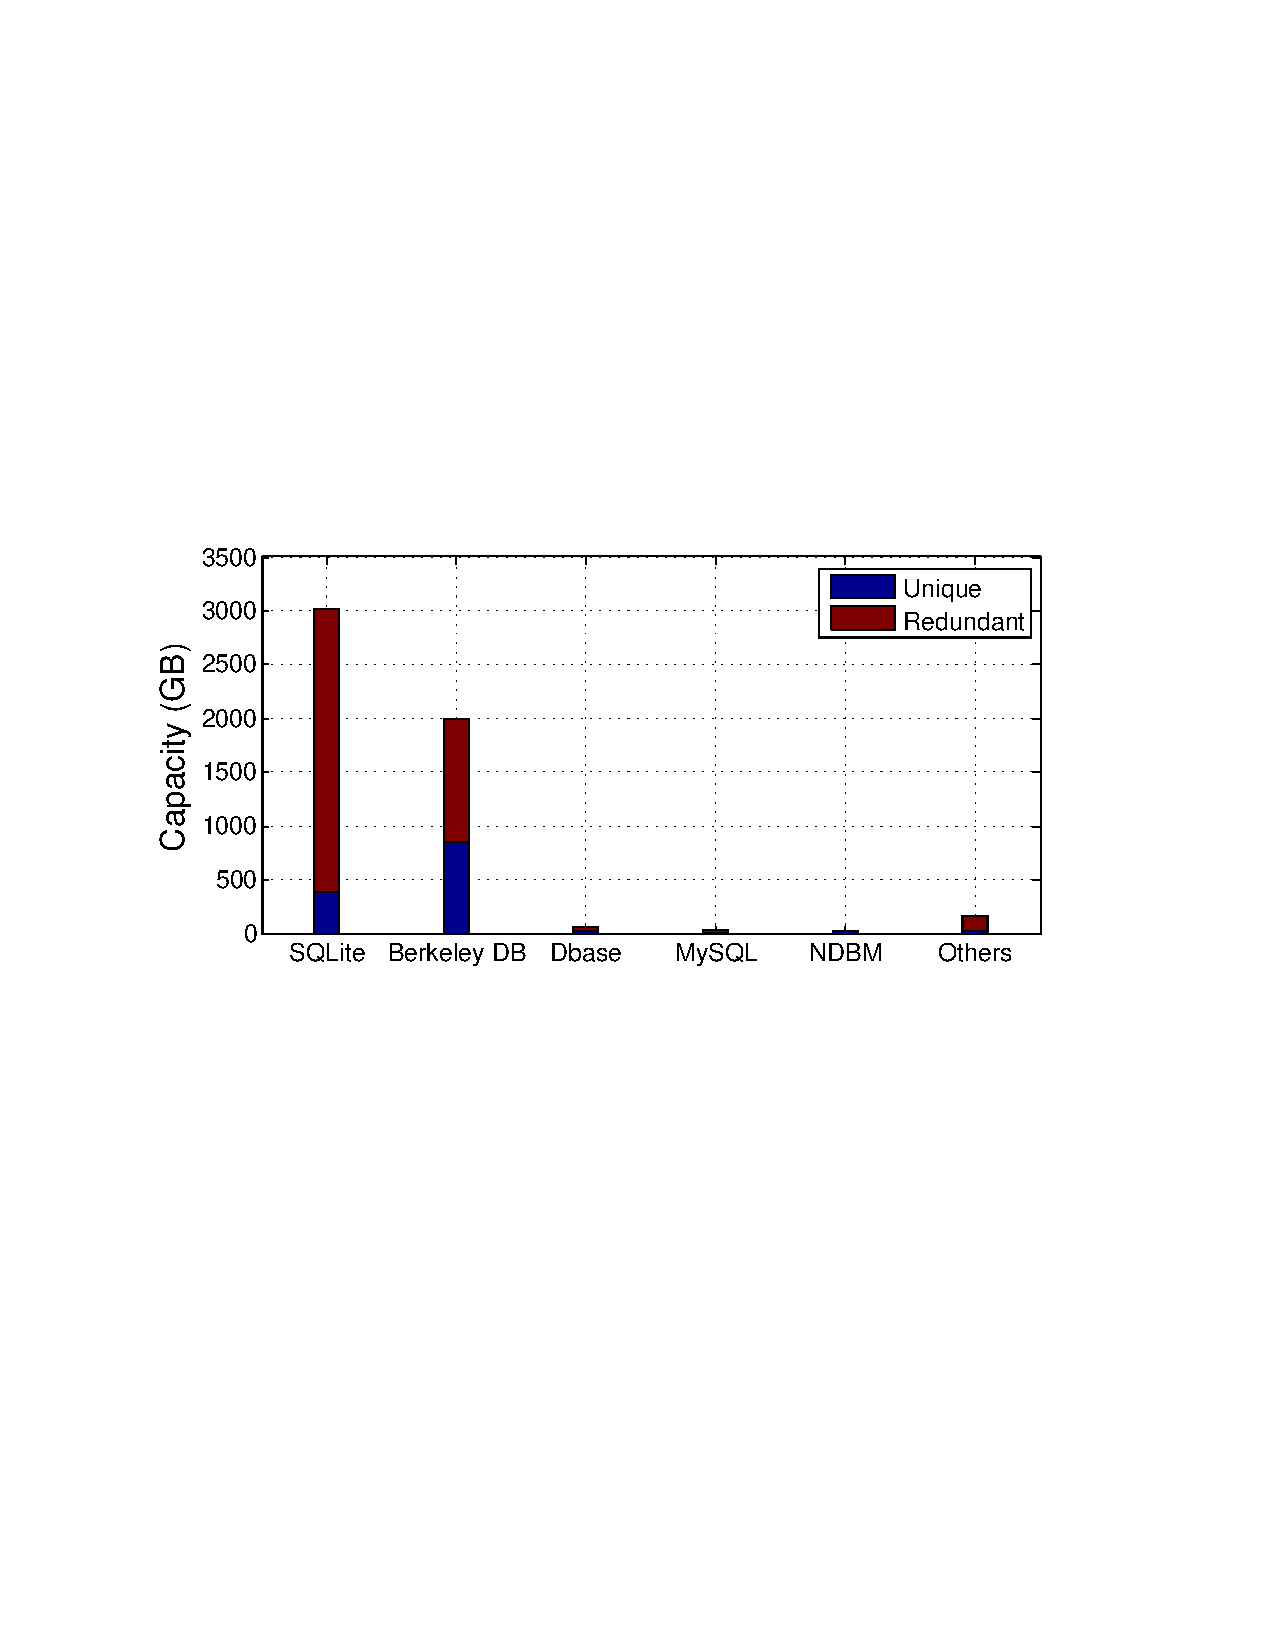
\includegraphics[width=1\textwidth]{graphs/type-db-cap.pdf} %
%%\caption{Redundant data vs. unique data for database related files} %
%%\label{fig:type-db} %	\end{minipage}% %
%%\begin{minipage}{0.278\textwidth} %		\centering %
%%\includegraphics[width=1\textwidth]{graphs/type-tar-type} %
%%\caption{Redundant data vs. unique data for archival files} %
%%\label{fig:type-arch} %	\end{minipage} %
%%\begin{minipage}{0.28\textwidth} %		\centering %
%%\includegraphics[width=1\textwidth]{graphs/type-image-cap} %
%%\caption{Redundant data vs. unique data for image files} %
%%\label{fig:type-img} %	\end{minipage} %\end{figure*}
%%
%%\paragraph{Archival (Arch.)}
%%
%%Figure~\ref{fig:type-arch} shows the deduplication ratio for each common
%%archival type.  We see that most of archival files have a high deduplication
%%over 80\% except tar archival files. Especially, Zip/Gzip files contribute to
%%most capacity savings after deduplication (62\%).  To understand why there are
%%so many redundant Zip/Gzip files, we manually inspected redundant Zip/Gzip
%%files and found that most of zip/Gzip files packages open source codes.  For
%%example, we found a redundant zip files called android-ndk-r12b.zip. It
%%packages the open source code--Android Native Development Kit (NDK)--that
%%allows Android application developers to include native code in their Android
%%application packages, compiled as JNI shared libraries~\cite{xxx}.
%%android-ndk-r12b.zip is available for downloading from GitHub. 
%%
%%\textit{Finding 9: Archival files have a high deduplication ratio. Majority of
%%Zip/Gzip files packages open source codes that are available online. We
%%suggest developers to remove the redundant archival files after unpacking to
%%reduce image size and save space.}
%%
%%%Finding 4: 89.5\% and 7.0\% of redundant archival files are Gzip files and
%%Zip files, which take up over 8.4 TB and 15.2 TB storage space, indicating
%%that users replicate more Gzip files and Zip files are much bigger than Gzip
%%files.  % % redundant archival file distribution. Gzip files have the largest
%%number of redundant archival files (89.5\%), which take up to 8TB storage
%%space, indicating that users replicate more Gzip compressed files. Although
%%Zip files only take 7.00\% of redundant archival files, they consume 15.5 TB
%%storage space since they are much bigger than Gzip files.  % %We found other
%%different kinds of archive files, such as XZ (0.42\%), Bzip2(0.96\%), and Tar
%%files(0.36\%).
%%
%\paragraph{Images (Img.)}
%
%\begin{figure} \centering
%\includegraphics[width=0.35\textwidth]{graphs/dedup-img} \caption{Deduplication
%results for image files.  } \label{fig:dedup-img} \end{figure}
%
%Last, we present the redundant ratio for image files as shown in
%Figure~\ref{fig:dedup-img}.  We see that most of image files have a high
%deduplication ratio over 80\% except TIFF image files and TIFF image files.
%Especially, PNG images contributes to almost half of capacity savings after
%deduplication.  To understand why there are so many redundant image files, we
%inspected redundant PNG images and found plenty of PNG images are logo, icons,
%wallpapers, and images for testing.  For example, we found plenty of redundant
%PNG images related to matplotlib~\cite{matplotlib} for testing purpose. matplotlib is
%a Python 2D plotting library and available on GitHub.
%
%\textit{Finding 10: Most image files have a high deduplication ratio. PNG files
%contribute most to the space savings. Majority redundant PNG files are
%supplementary for documents or testing images for graphic editor softwares.}
%%%Finding 4: 67.8\%, 14.3\%, and 4.0\% of redundant image files are PNG, SVG,
%%and JPEG images, which take up over 1.01TB, 4.6 GB, and 401.5 GB storage
%%space, indicating that users also replicate image files, especially, PNG, SVG,
%%and JPEG files.  % % shows the redundant image file distribution. PNG image
%%files have the largest number of redundant image files (67.8\%), which take up
%%to over 1 TB storage space. 14.3\%, and 4.0\% of redundant image files are
%%SVG, and JPEG images, which take up over 4.6 GB and 401.5 GB storage space,
%%indicating that users also replicate image files, especially, PNG, SVG, and
%%JPEG files. Moreover, there are different redundant image file types, such as
%%FITS (0.05\%), TIFF (0.07\%), and EPS (0.01\%) image files.
%%
%%%\begin{figure} %	\centering %
%%\includegraphics[width=0.35\textwidth]{graphs/type-utili-cap} %
%%\caption{Image file distribution.  %	} %	\label{fig:file_size}
%%%\end{figure}
%%
%%%======================================= %|             OLD VERSION
%%| %=======================================
%%
%%%\begin{table} %	\centering %	\scriptsize  %	\caption{Top 20
%%redundant files' characterization (sorted by repeat cnt.)} %
%%\label{tbl:top_dup_files_repeat_cnt} %
%%\begin{tabular}{|l|l|l|l|l|}%p{0.14\textwidth} %		\hline %
%%Filename & repeat cnt. & type & extension & size \\ %		\hline %
%%&   &   &   &  \\ %		\hline %		&   &   &   &   \\ %
%%\hline %		&   &   &  &    \\ %		\hline %
%%&  &  &  & \\ %		\hline %		& &  &   & \\ %
%%\hline %		& &  &   & \\ %		\hline %		&  &  &
%%& \\ %		\hline %	\end{tabular} %\end{table}
%%
%%%\begin{table} %	\centering %	\scriptsize  %	\caption{Top 20
%%redundant files' characterization (sorted by capacity)} %
%%\label{tbl:top_dup_files_cap} %
%%\begin{tabular}{|l|l|l|l|l|}%p{0.14\textwidth} %		\hline %
%%Filename & repeat cnt. & type & extension & size \\ %		\hline %
%%&   &   &   &  \\ %		\hline %		&   &   &   &   \\ %
%%\hline %		&   &   &  &    \\ %		\hline %
%%&  &  &  & \\ %		\hline %		& &  &   & \\ %
%%\hline %		& &  &   & \\ %		\hline %		&  &  &
%%& \\ %		\hline %	\end{tabular} %\end{table}
%%
%%
%%%\begin{table} %	\centering %	\scriptsize  %	\caption{Top redundant
%%file types} %	\label{tbl:top_dup_types} %
%%\begin{tabular}{|l|l|l|l|l|l|}%p{0.14\textwidth} %		\hline %
%%Type & extension & Num. & size & red. ratio (cnt.)  & red. ratio (cap.)\\ %
%%\hline %		&   &   &  & &   \\ %		\hline %
%%&   &   &  & &    \\ %		\hline %		&   &   &   & &   \\ %
%%\hline %		&  &  &  & & \\ %		\hline %
%%& &  &  & & \\ %		\hline %		& &  & & &  \\ %
%%\hline %		&  &  & & &  \\ %		\hline %
%%\end{tabular} %\end{table} 
%%
%%%\subsection{Redundant ratio for directories} % %\begin{table} %
%%\centering %	\scriptsize  %	%\begin{minipage}{.5\linewidth} %
%%\caption{Inter-dir redundant ratio for dirs in terms of file count and
%%capacity} \label{tbl:intra_dup_ratio_dirs} %
%%\begin{tabular}{|l|l|l|}%p{0.14\textwidth} %		\hline %
%%% after \\: \hline or \cline{col1-col2} \cline{col3-col4} ...  %
%%% after \\: \hline or \cline{col1-col2} \cline{col3-col4} ...  %
%%& File count & Capacity \\ %		\hline %		Avg. & 98.75\%
%%& 97.33\%\\ %		\hline %		Median & - & - \\ %
%%\hline %		Max. & 1 & 1\\ %		\hline %
%%Min.  & 0.87\%  & $<$ 0.00\%\\ %		\hline %		Stdev.
%%&  4.70\% & 10.49\\ %		\hline %		Layer dataset after
%%share.-dedup (Uncompressed) & -  & -\\ %		\hline %
%%Total layer dataset (Uncompressed) &  -	& -\\ %		\hline %
%%\end{tabular} %\end{table} % %\begin{table} %	\centering %	\scriptsize  %
%%%\begin{minipage}{.5\linewidth} %	\caption{Intra-dir redundant ratio for
%%dirs in terms of file count and capacity} \label{tbl:inter_dup_ratio_dirs} %
%%\begin{tabular}{|l|l|l|}%p{0.14\textwidth} %		\hline %
%%% after \\: \hline or \cline{col1-col2} \cline{col3-col4} ...  %
%%% after \\: \hline or \cline{col1-col2} \cline{col3-col4} ...  %
%%& File count & Capacity \\ %		\hline %		Avg. & 98.75\%
%%& 97.33\%\\ %		\hline %		Median & - & - \\ %
%%\hline %		Max. & 1 & 1\\ %		\hline %
%%Min.  & 0.87\%  & $<$ 0.00\%\\ %		\hline %		Stdev.
%%&  4.70\% & 10.49\\ %		\hline %		Layer dataset after
%%share.-dedup (Uncompressed) & -  & -\\ %		\hline %
%%Total layer dataset (Uncompressed) &  -	& -\\ %		\hline %
%%\end{tabular} %\end{table}
%%
%%%\subsection{Redundant directory characterization} % %\begin{table} %
%%\centering %	\scriptsize  %	%\begin{minipage}{.5\linewidth} %
%%\caption{Top redundant dirs'characterization} %
%%\label{tbl:top_dup_dirs} %	\begin{tabular}{|l|l|l|l|}%p{0.14\textwidth} %
%%\hline %		% after \\: \hline or \cline{col1-col2}
%%\cline{col3-col4} ...  %		% after \\: \hline or \cline{col1-col2}
%%\cline{col3-col4} ...  %		Name & Num. & Redundant ratio & Avg.
%%size \\ %		\hline %		home &   &   &     \\ %
%%\hline %		&   &   &      \\ %		\hline %
%%&   &   &      \\ %		\hline %		&  &  &  \\ %
%%\hline %		& &  &   \\ %		\hline %		& &  &
%%\\ %		\hline %		&  &  & \\ %		\hline %
%%\end{tabular} %\end{table} 
%%
%%%\begin{figure} %	\centering %
%%\includegraphics[width=0.5\textwidth]{graphs/} %	\caption{CDF of file
%%repeat count.  %	} %	\label{fig:file_repeat_count} %\end{figure}
%%
%%%\paragraph{Cumulative distribution and probability distribution of file size
%%in terms of unique file size, redundant file size, overall file size}
%%
%%
%%%\paragraph{Average file size by repeat count} % %There is no relation between
%%file repeat count and average file size.  % %\begin{figure} %	\centering %
%%\includegraphics[width=0.5\textwidth]{graphs/avg_size_by_cnt.eps} %
%%\caption{Average file size with same repeat count.  %	} %
%%\label{fig_avg_size_by_cnt} %\end{figure} % %\paragraph{Redundant ratio by
%%file size for the files with the same content in terms of file count and
%%storage capacity} %Total size of redundant files with same content(TRS) %
%%%97\% of the TRSs are equal or less than 100MB.  % %\begin{figure} %
%%\centering %
%%\includegraphics[width=0.5\textwidth]{graphs/Total_size_of_redudant_files_with_same_content-KB.eps}
%%%	\caption{CDF of total file size with same file content (MB).  %	} %
%%\label{fig_total_redundant_same_digest} %\end{figure} % %\paragraph{Redundant
%%ratio by repeat count for the files with the same repeat count in terms of
%%file count and storage capacity} % %However, with the increase of file repeat
%%count, the sum of file size with same repeat count becomes smaller.  %
%%%\begin{figure} %	\centering %
%%\includegraphics[width=0.5\textwidth]{graphs/sum_size_by_cnt.eps} %
%%\caption{Sum of file size with same repeat count.  %	} %
%%\label{fig_sum_by_cnt} %\end{figure}
%%
%%% %\paragraph{Cumulative distribution and probability distribution of file
%%repeat count} %\begin{table} %	\centering %	\scriptsize  %
%%%\begin{minipage}{.5\linewidth} %	\caption{Summary of image types}
%%\label{tbl:redundant_ratio} %	\begin{tabular}{|l|l|l|}%p{0.14\textwidth} %
%%\hline %		% after \\: \hline or \cline{col1-col2}
%%\cline{col3-col4} ...  %		% after \\: \hline or \cline{col1-col2}
%%\cline{col3-col4} ...  %		Image types & num. & avg. redundant
%%ratio  \\ %		\hline %		  &   &        \\ %
%%\hline %		  &   &         \\ %		\hline %
%%&   &       \\ %		   \hline %		other     &   &
%%\\ %		\hline %	\end{tabular} %\end{table}
%%
%%%\subsection{Redundant files with same filename and relative path} %
%%%\subsection{Common directories that contains redundant files} %
%%%\subsection{Redundant tar files} %\begin{table} %	\centering %
%%\scriptsize  %	%\begin{minipage}{.5\linewidth} %	\caption{Summary of
%%file \& dir. characterization} \label{tbl:sum_file_dir_char} %
%%\begin{tabular}{|l|l|l|l|l|}%p{0.14\textwidth} %		\hline %
%%% after \\: \hline or \cline{col1-col2} \cline{col3-col4} ...  %
%%% after \\: \hline or \cline{col1-col2} \cline{col3-col4} ...  %
%%Metrics & max & min & median & avg.\\ %		\hline %
%%File size &   &   &   &  \\ %		\hline %		File size
%%(repeat cnt. $>$ 1) &   &   &    &  \\ %		\hline %
%%File size (repeat cnt. $=$ 1) &   &   &    &  \\ %		\hline %
%%\hline %		Dir. size &  &  & & \\ %		\hline %
%%File cnt. per dir & &  &  & \\ %		\hline %
%%Redundant ratio & &  &  & \\ %		\hline %		Dir. depth  &
%%&  & & \\ %		\hline %	\end{tabular} %\end{table} 


%\section{Redundant file characterization}
\label{sec:redundant_files}

\begin{figure*}
	\centering
	\includegraphics[width=1\textwidth]{graphs/graph-types-hierarchy}
	\caption{Taxonomy of file types.
	}
	\label{fig:file-type-hierarchy}
\end{figure*}

In this section, we present our redundant file characterization on file repeat count, file size, and file types. 
Based on this characterization, we create three-level classification hierarchy as shown in Figure~\ref{fig:file-type-hierarchy}.
At the highest level, we created two categories: \textit{common redundant file types and non-common redundant file types}. 
The majority (xxxx\% files, with xxx TB) are common file types that consists of a largest number of redundant files with large storage space consumed, such as xxx and xxx. 
Only xxxx\% files are non-common file types that only contains a small number of redundant files with less storage space, such as xxxx and xxxx. 
Since our focus is on the major redundant files, our further classification expands on the xxx\% common redundant file types.  

At the second level of the hierarchy, we clustered common redundant file types based on the \textit{major usage, platform, or framework} involved by each file type. We identified redundant files' types relevant to \textit{archival, productivity, programming languages, scripts, images, databases, executables, and others}.

At the third level, we classified the redundant files based on the specific file type or extension. Totally, we get around 1500 types. 

133 file types that redundant capacity $>$ 5G 
%We selected the file types which take largest storage space.  

Based on the second-and third-level classification, we further investigated the following two research questions: (1) What are the common redundant files?
(2) Why there are so many redundant files? and present our investigation results.

\begin{figure}
	\centering
	\includegraphics[width=0.5\textwidth]{graphs/File_repeat_count.eps}
	\caption{File repeat count distribution.
	}
	\label{fig:file-repeat-cnt}
\end{figure}

Figure~\ref{fig:file-repeat-cnt} shows the cumulative and probability distribution of file repeat count. 
Most files have a small repeat count. For instance, almost 90\% of files have equal or less than 10 copies. Around 50\% of files have 4 copies.
The file that has the maximum repeat count is empty file, which means that many users creates empty files and stored in their images.
%\subsection{File repeat count}
%\subsection{File size}

\begin{figure}
	\centering
	\includegraphics[width=0.5\textwidth]{graphs/File_size-KB.eps}
	\caption{File size distribution.
	}
	\label{fig:file-size}
\end{figure}

Figure~\ref{fig:file-size} shows the cumulative and probability distribution of file size of unique dataset after we remove the redundant files.
Most files are smaller files. For example, 91\% files'sizes are equal or less than 100KB. 
Around 22\% of files are less than 1 KB.
 

\subsection{Overview of high redundant file types}

\paragraph{Finding 1: \%, \% of redundant files are source codes and EOL files, which take up over \%, \% of redundant storage capacity, indicating that users are more prone to replicate source codes and create identical big EOF files, while \%, \% of redundant files are documents and archival files, which account for \%, \% of redundant storage capacity, indicating users replicates or creates identical documents and archival files}

%Some data is inherently more prone to duplicates than others.
Figure~\ref{fig:file-types} presents redundant data vs. unique data for each clusters. 
Document cluster has the largest number of redundant files, indicating that users replicate or create more identical documents. While the redundant document files only consume xxx (xxx\%) of storage space, indicating that the size of redundant document files are small. In comparison, \% and \% of files are EOL files and source codes, which take up over \%, \% of redundant storage capacity, indicating that users replicate source codes and create identical big EOF files.

Archival files and scripts have almost similarly number of redundant files, xxx for archival and xxx for scripts. However, archival cluster consumes xxxx more than that of scripts since archival file size is inherently higher than script size.

We found that xxx of files are image files and xxx of files are relevant to database, which takes xxx, xxx of storage space respectively. There are xxx (xxx TB) of redundant files in Other cluster which contains, xxx, xxx, xxx, etc. 

\begin{figure}
	\centering
	\subfigure[Redundant data vs. unique data in terms of file count.]{\label{fig:file-types-cnt}
		\includegraphics [width=0.4\textwidth]{graphs/type-total-cnt}
	}
	\subfigure[Redundant data vs. unique data in terms of capacity.]{\label{fig:file-types-cap}
		\includegraphics [width=0.4\textwidth]{graphs/type-total-cap}
	}
	\caption{Redundant data vs. unique data for high redundant file types}
	\label{fig:file-types}
\end{figure}

\subsection{EOL files and source codes}

\paragraph{Finding 2: 31.4\% (164,059,690) and 63.7\% (333,261,220) of EOL files are ELF files and intermediate compiled files, which take up over 85.7\% (45.3TB) and 5.3\% (2.8TB) of redundant storage capacity, indicating that users replicate or create more identical ELF files and intermediate compiled files. 64.1\% (213,753,591) of intermediate compiled files are Python byte-compiled files, which take up to 79.4\% (2.2TB) of redundant storage space, indicating that users compiled more Python scripts (similar to Finding 2.)}

As shown in Figure~\ref{fig:type-eol}, intermediate compiled files have the largest number of redundant copies (333,261,220, 63.7\%), which only take up to 5.3\% (2.8TB) of EOL redundant storage space, indicating that users creates more small redundant intermediate compiled files. Among all the intermediate compiled files, python byte-compiled files have the largest number of redundant copies (64.1\%, 213,753,591), which account for 79.4\% (2.2TB) of EOL redundant storage space as shown in Figure~\ref{fig:type-compiled}. 

We found that there are various redundant intermediate compiled files in layers in addition to Python byte-compiled, such as Erlang beam files, Xemacs/emacs compiled files, compiled Java class, Mach-o fat files, Guile object bytecode, and llvm bitcode files. We see that 21.6\% (71,830,155) and 10.12\% (33,740,399) of redundant intermediate compiled files are terminfo compiled and compiled java class files, which consume 76.4 GB and 104.4 GB storage space.   

%ELF files have the largest redundant capacity
%A large executable group is ELF file type, which consists of ELF 64/32-bit LSB relocatable, shared object, executable, core file, processor-specific for x86-64, MIPS,
%ARM, Intel 80386, etc. architectures.
%Another executable group contains VAX COFF executable, PE32/PE32+ executable for Windows, and 386 pure executable, VMS Alpha, etc.
%\% of files are script executable, which contains python, shell, etc.
%\% of files are RPM, Debian bin

\paragraph{Finding 3: 80.2\% (548,507,865) of source codes are C/C++ source, which take up to 79.7\% (4.2TB) of redundant storage space, indicating that users are more prone to duplicate C/C++ codes, which results in more ELF file replicas.}
%The last group contains

\begin{figure}
	\centering
	\includegraphics[width=0.5\textwidth]{graphs/type-exec-cap}
	\caption{Redundant data vs. unique data for EOL (Executable, object code, libraries) files.
	}
	\label{fig:type-eol}
\end{figure}

Figure~\ref{fig:type-source} shows the redundant file count and storage capacity distribution for source code. C/C++ source codes have the largest number of redundant files. 80.2\% (548,507,865) of source codes are C/C++ source, which take up to 79.7\% (4.2TB) of redundant storage space, indicating that users are more prone to duplicate C/C++ codes, which results in more ELF file replicas.

We also found other source codes, such as Perl5 module source code (9.5\%), ruby module source code (7.6\%), assembler source code (1.1\%), pascal source (0.7\%), fortran program code (0.01\%), applesoft basic source code, and Lisp/scheme source code (0.17\%).

\begin{figure}
	\centering
	\includegraphics[width=0.5\textwidth]{graphs/type-lang-cap}
	\caption{Redundant data vs. unique data for source code files.
	}
	\label{fig:type-source}
\end{figure}

Figure~\ref{fig:type-lib} shows the redundant library distribution. We see that Gcc precompiled header files have the lowest number of redundant library files (20.3\%), but they take up to 0.93 TB. Almost 86.4\% of redundant library files are Palm libraries, which only take up to 7.2GB space, indicating that gcc compiled header files are much bigger than other libraries.

We also found there are different libraries used in layers, such as netcdf library, Ocaml lib., mach-o lib.

%Figure~\ref{fig-elf}
%\subsection{Lib}
%
%library files contains libtool library file, OCaml native library, MIT scheme, Mach-O library, OCaml library, Palm OS dynamic library data, Microsoft c/c++ library.current ar archive random library, and other library.
%%libtool\|OCaml\|Palm\|MIT\|microsoft\|current ar archive random library\|mach-o\|rpm\|gzip

%\subsection{Source code}

\subsection{Scripts}
\paragraph{Finding 2: 53.6\% (238,353,674) of redundant scripts are Python scripts, which take up over 2.6TB storage space, indicating that users are more prone to replicate Python scripts compare to other scripts}

\begin{figure}
	\centering
	\includegraphics[width=0.5\textwidth]{graphs/type-script-cap}
	\caption{Redundant data vs. unique data for scripts.
	}
	\label{fig:type-script}
\end{figure}

Figure~\ref{fig:type-script} shows the redundant scripts distribution. Python script has the largest number of redundant scripts (238353674, 53.6\%), which take up to 2.6TB storage space, indicating that users are more prone to replicate Python scripts compare to other scripts. 
%This finding also explains that why python byte compiled files takes the largest proportion of intermediate 

We find that users use different scripts in the images. 
For example, 20\%, 9.7\% and 4.4\% of scripts are bash/shell scripts, ruby scripts, and awk scripts. Other scripts such as perl script (4.2\%), php script(3.9\%), makefile script(1.3\%), and M4 macro processor script(0.7\%) are also used.

\subsection{Documents}
\paragraph{Finding 3: 79.7\%, 5.2\%, and 12.4\% of redundant documents are ASCII text, UTF-8/16 text, and HTML/XML/XHTML, which take up over 11TB, 3.4TB, and 3.9TB redundant storage, indicating that users replicate more ASCII text, UTF-8/16 text, and HTML/XML/XHTML compare to other documents}

\begin{figure}
	\centering
	\includegraphics[width=0.5\textwidth]{graphs/type-utili-cap}
	\caption{Redundant data vs. unique data for documents.
	}
	\label{fig:type-doc}
\end{figure}

Figure~\ref{fig:type-doc} presents redundant document distribution. We first group documents into two categories: non-text documents and raw text documents. 
We see that ASCII text files have the largest number of redundant document files (1,758,299,693, 79.7\%), which take up to 11TB storage space, indicating that users replicate more ASCII text. 
12.4\% of the redundant documents are HTML/XML/XHTML documents, which take up to 3.9 TB storage space, indicating users also replicate HTML/XML/XHTML documents in images.  

In addition to ASCII text, 5.2\% of redundant documents are UTF-8/16 unicode text, which take up 3.4 TB storage space.
Various documents are replicated in images, such as PS/PDF documents (0.9\%), LaTex files (1.1\%) and Composite documents (0.01\%)

%79.7\%, 5.2\%, and 12.4\% of redundant documents are ASCII text, UTF-8/16 text, and HTML/XML/XHTML, which take up over 11TB, 3.4TB, and 3.9TB redundant storage, indicating that users replicate more ASCII text, UTF-8/16 text, and HTML/XML/XHTML compare to other documents.
%type-utili-cap
%type-script-cap

\subsection{Database related files}
\paragraph{Finding 4: 28.7\%, 30.9\%, and 11.9\% of redundant database files are Berkeley DB, Mysql, and Dbase related files, which only take up over 1.1 TB, 26 GB, and 47.2 GB redundant storage, indicating that users replicate database files, especially, SQLite and Berkeley DB. While there are only 7.3\% of SQLite files, which take up over 2.6TB storage space, indicating SQLite files are much bigger than others}




\begin{figure*}[t]
	\centering
	\begin{minipage}{0.35\textwidth}
		\centering
		\includegraphics[width=1\textwidth]{graphs/type-db-cap.pdf}
		\caption{Redundant data vs. unique data for database related files}
		\label{fig:type-db}
	\end{minipage}%
	\begin{minipage}{0.278\textwidth}
		\centering
		\includegraphics[width=1\textwidth]{graphs/type-tar-type}
		\caption{Redundant data vs. unique data for archival files}
		\label{fig:type-arch}
	\end{minipage}
	\begin{minipage}{0.28\textwidth}
		\centering
		\includegraphics[width=1\textwidth]{graphs/type-image-cap}
		\caption{Redundant data vs. unique data for image files}
		\label{fig:type-img}
	\end{minipage}
\end{figure*}

\subsection{Archival}
\paragraph{Finding 4: \% and \% of archival files are Zip files and Gzip files, which take up over \% and \% of redundant storage capacity, indicating that users also replicate or create archival files, especially, Zip and Gzip files}

\subsection{Images}
\paragraph{Finding 4: \% and \% of image files are PNG and JPEG text, which take up over \% and \% of redundant storage capacity, indicating that users also replicate image files, especially, PNG and JPEG files}
%\begin{figure}
%	\centering
%	\includegraphics[width=0.35\textwidth]{graphs/type-utili-cap}
%	\caption{Image file distribution.
%	}
%	\label{fig:file_size}
%\end{figure}

%=======================================
%|             OLD VERSION              |
%=======================================

%\begin{table} 
%	\centering 
%	\scriptsize  
%	\caption{Top 20 redundant files' characterization (sorted by repeat cnt.)}
%	\label{tbl:top_dup_files_repeat_cnt} 
%	\begin{tabular}{|l|l|l|l|l|}%p{0.14\textwidth} 
%		\hline 
%		Filename & repeat cnt. & type & extension & size \\
%		\hline
%		&   &   &   &  \\
%		\hline
%		&   &   &   &   \\
%		\hline
%		&   &   &  &    \\
%		\hline
%		&  &  &  & \\
%		\hline
%		& &  &   & \\
%		\hline
%		& &  &   & \\
%		\hline
%		&  &  & & \\
%		\hline
%	\end{tabular} 
%\end{table}

%\begin{table} 
%	\centering 
%	\scriptsize  
%	\caption{Top 20 redundant files' characterization (sorted by capacity)} 
%	\label{tbl:top_dup_files_cap} 
%	\begin{tabular}{|l|l|l|l|l|}%p{0.14\textwidth} 
%		\hline 
%		Filename & repeat cnt. & type & extension & size \\
%		\hline
%		&   &   &   &  \\
%		\hline
%		&   &   &   &   \\
%		\hline
%		&   &   &  &    \\
%		\hline
%		&  &  &  & \\
%		\hline
%		& &  &   & \\
%		\hline
%		& &  &   & \\
%		\hline
%		&  &  & & \\
%		\hline
%	\end{tabular} 
%\end{table}


%\begin{table} 
%	\centering 
%	\scriptsize  
%	\caption{Top redundant file types} 
%	\label{tbl:top_dup_types} 
%	\begin{tabular}{|l|l|l|l|l|l|}%p{0.14\textwidth} 
%		\hline 
%		Type & extension & Num. & size & red. ratio (cnt.)  & red. ratio (cap.)\\
%		\hline
%		&   &   &  & &   \\
%		\hline
%		&   &   &  & &    \\
%		\hline
%		&   &   &   & &   \\
%		\hline
%		&  &  &  & & \\
%		\hline
%		& &  &  & & \\
%		\hline
%		& &  & & &  \\
%		\hline
%		&  &  & & &  \\
%		\hline
%	\end{tabular} 
%\end{table} 

%\subsection{Redundant ratio for directories}
%
%\begin{table} 
%	\centering 
%	\scriptsize  
%	%\begin{minipage}{.5\linewidth}
%	\caption{Inter-dir redundant ratio for dirs in terms of file count and capacity} \label{tbl:intra_dup_ratio_dirs} 
%	\begin{tabular}{|l|l|l|}%p{0.14\textwidth} 
%		\hline 
%		% after \\: \hline or \cline{col1-col2} \cline{col3-col4} ... 
%		% after \\: \hline or \cline{col1-col2} \cline{col3-col4} ... 
%		& File count & Capacity \\
%		\hline
%		Avg. & 98.75\% & 97.33\%\\
%		\hline
%		Median & - & - \\
%		\hline
%		Max. & 1 & 1\\
%		\hline
%		Min.  & 0.87\%  & $<$ 0.00\%\\
%		\hline
%		Stdev.  &  4.70\% & 10.49\\
%		\hline
%		Layer dataset after share.-dedup (Uncompressed) & -  & -\\
%		\hline 
%		Total layer dataset (Uncompressed) &  -	& -\\
%		\hline
%	\end{tabular} 
%\end{table}
%
%\begin{table} 
%	\centering 
%	\scriptsize  
%	%\begin{minipage}{.5\linewidth}
%	\caption{Intra-dir redundant ratio for dirs in terms of file count and capacity} \label{tbl:inter_dup_ratio_dirs} 
%	\begin{tabular}{|l|l|l|}%p{0.14\textwidth} 
%		\hline 
%		% after \\: \hline or \cline{col1-col2} \cline{col3-col4} ... 
%		% after \\: \hline or \cline{col1-col2} \cline{col3-col4} ... 
%		& File count & Capacity \\
%		\hline
%		Avg. & 98.75\% & 97.33\%\\
%		\hline
%		Median & - & - \\
%		\hline
%		Max. & 1 & 1\\
%		\hline
%		Min.  & 0.87\%  & $<$ 0.00\%\\
%		\hline
%		Stdev.  &  4.70\% & 10.49\\
%		\hline
%		Layer dataset after share.-dedup (Uncompressed) & -  & -\\
%		\hline 
%		Total layer dataset (Uncompressed) &  -	& -\\
%		\hline
%	\end{tabular} 
%\end{table}

%\subsection{Redundant directory characterization}
%
%\begin{table} 
%	\centering 
%	\scriptsize  
%	%\begin{minipage}{.5\linewidth}
%	\caption{Top redundant dirs'characterization} 
%	\label{tbl:top_dup_dirs} 
%	\begin{tabular}{|l|l|l|l|}%p{0.14\textwidth} 
%		\hline 
%		% after \\: \hline or \cline{col1-col2} \cline{col3-col4} ... 
%		% after \\: \hline or \cline{col1-col2} \cline{col3-col4} ... 
%		Name & Num. & Redundant ratio & Avg. size \\
%		\hline
%		home &   &   &     \\
%		\hline
%		&   &   &      \\
%		\hline
%		&   &   &      \\
%		\hline
%		&  &  &  \\
%		\hline
%		& &  &   \\
%		\hline
%		& &  &   \\
%		\hline
%		&  &  & \\
%		\hline
%	\end{tabular} 
%\end{table} 

%\begin{figure}
%	\centering
%	\includegraphics[width=0.5\textwidth]{graphs/}
%	\caption{CDF of file repeat count.
%	}
%	\label{fig:file_repeat_count}
%\end{figure}

%\paragraph{Cumulative distribution and probability distribution of file size in terms of unique file size, redundant file size, overall file size}


%\paragraph{Average file size by repeat count}
%
%There is no relation between file repeat count and average file size.
%
%\begin{figure}
%	\centering
%	\includegraphics[width=0.5\textwidth]{graphs/avg_size_by_cnt.eps}
%	\caption{Average file size with same repeat count.
%	}
%	\label{fig_avg_size_by_cnt}
%\end{figure}
%
%\paragraph{Redundant ratio by file size for the files with the same content in terms of file count and storage capacity}
%Total size of redundant files with same content(TRS)
%
%97\% of the TRSs are equal or less than 100MB.
%
%\begin{figure}
%	\centering
%	\includegraphics[width=0.5\textwidth]{graphs/Total_size_of_redudant_files_with_same_content-KB.eps}
%	\caption{CDF of total file size with same file content (MB).
%	}
%	\label{fig_total_redundant_same_digest}
%\end{figure}
%
%\paragraph{Redundant ratio by repeat count for the files with the same repeat count in terms of file count and storage capacity}
%
%However, with the increase of file repeat count, the sum of file size with same repeat count becomes smaller.
%
%\begin{figure}
%	\centering
%	\includegraphics[width=0.5\textwidth]{graphs/sum_size_by_cnt.eps}
%	\caption{Sum of file size with same repeat count.
%	}
%	\label{fig_sum_by_cnt}
%\end{figure}

%
%\paragraph{Cumulative distribution and probability distribution of file repeat count}
%\begin{table} 
%	\centering 
%	\scriptsize  
%	%\begin{minipage}{.5\linewidth}
%	\caption{Summary of image types} \label{tbl:redundant_ratio} 
%	\begin{tabular}{|l|l|l|}%p{0.14\textwidth} 
%		\hline 
%		% after \\: \hline or \cline{col1-col2} \cline{col3-col4} ... 
%		% after \\: \hline or \cline{col1-col2} \cline{col3-col4} ... 
%		Image types & num. & avg. redundant ratio  \\
%		\hline
%		  &   &        \\
%		\hline
%		  &   &         \\
%		\hline
%		   &   &       \\
%		   \hline
%		other     &   &       \\
%		\hline
%	\end{tabular} 
%\end{table}

%\subsection{Redundant files with same filename and relative path}
%
%\subsection{Common directories that contains redundant files}
%
%\subsection{Redundant tar files}
%\begin{table} 
%	\centering 
%	\scriptsize  
%	%\begin{minipage}{.5\linewidth}
%	\caption{Summary of file \& dir. characterization} \label{tbl:sum_file_dir_char} 
%	\begin{tabular}{|l|l|l|l|l|}%p{0.14\textwidth} 
%		\hline 
%		% after \\: \hline or \cline{col1-col2} \cline{col3-col4} ... 
%		% after \\: \hline or \cline{col1-col2} \cline{col3-col4} ... 
%		Metrics & max & min & median & avg.\\
%		\hline
%		File size &   &   &   &  \\
%		\hline
%		File size (repeat cnt. $>$ 1) &   &   &    &  \\
%		\hline
%		File size (repeat cnt. $=$ 1) &   &   &    &  \\
%		\hline
%		\hline
%		Dir. size &  &  & & \\
%		\hline
%		File cnt. per dir & &  &  & \\
%		\hline
%		Redundant ratio & &  &  & \\
%		\hline
%		Dir. depth  &  &  & & \\
%		\hline
%	\end{tabular} 
%\end{table} 
%\section{Image characterization}
\label{sec:redundant_images}

\subsection{Layer count}

\subsection{Image size}

\subsection{Compression ratio}

\subsection{Directory count}


\subsection{File count}




\section{Registry with deduplication support}
\label{sec:file_adressable}

%Our analysis in Section~\ref{sec:redundant_files} suggests that adding the
%support of file-level deduplication to Docker registry can significantly reduce
%its storage capacity requirements, especially in large-scale deployments.
%
In this section, we first describe a high-level design of \emph{\sysname}---
a Docker registry that supports file-level deduplication.
We then proceed with a simulation-based evaluation of the expected performance
implications.

\vspace{-4pt}
\subsection{Registry Deduplication \& Caching}
\label{sec:design}
\vspace{-4pt}

%\sysname\ performs file-level deduplication for a Docker registry.
%

%We designed \sysname\ so that the interface between the Docker clients and the
%registry remains unchanged.
%
%As such, no modifications to the Docker clients are needed.
%
%Below we describe how \sysname\ handles layer pushes and
%pulls at the registry side.
%
%For the sake of this paper, we explain only the main steps omitting smaller
%details.
%\Ali{Following text makes no sense.. what are you trying to explain??}
%\NZ{This part includes our architecture. Our architecture doesn't required many words to explain}
%
%Traditionally, Docker registry is a web server that serves Docker
%\texttt{pull} and Docker \texttt{push} requests.  Although Docker registry is a
%layer-level content addressable storage system holding all the images, it
%delegates storage to drivers which interact with either a local file system or
%a remote cloud storage like S3~\cite{xxx}, Microsoft Azure~\cite{xxxx}, OpenStack Swift~\cite{xxx}, and Aliyun
%OSS~\cite{xxx} as shown in Figure~\ref{fig:sys-overview}.
%Deduplication methods are implemented on remote cloud storage servers or data centers to
%transparently remove duplicates from the incoming data stream.

%proxy caches, or web/HTTP caches 
%Modern container registries such as Google Container Registry~\cite{GoogleContainerRegistry} use cloud storage as their backend Docker image storage systems. 
%Users push and pull Docker images to and from their repositories stored on cloud storage. 
%
%To facilitate a fast and high-availability service, container registries use regional private repositories across the world.  
%This geographical distribution allows users to store images close to their compute instances and experience a fast response time. 
%For example, IBM's Container Registry setup spans five regions~\cite{dockerworkload}. 

%caches are placed as close to the requesting client as possible,
%such caches are known as for the temporary
%storage of frequently requested data to reduce the server's lag.  They are
%typically deployed in a regional ISP or within a corporate network.

\sysname~seamlessly integrates 
%the management of 
caching and deduplication on the
backend storage system (\emph{backend dedup storage}) with Docker registries.
%
We address a set of unique challenges to enable this integration.
%
First, for caching layers, \texttt{pull} layer requests are difficult to
predict because layers are accessed infrequently.
In~\cref{sec:background},
%\arb{???}, 
we have observed that about half of the layers are not
accessed again for at least $1.3$~hours. This means that if we
cache a layer, we may need to wait a long time before we observe a hit on that layer (as discussed in~\cref{sec:background}).  
This is mainly 
because when a user pulls an image from the registry, the Docker daemon on the
requesting host will only pull the layers that are not locally stored.
%\Ali{I do not understand the following sentence.}
%Moreover, we have to consider that a user might deploy an applications on
%multiple machines, so it's not easy to predict when a user will access which layers. 
%%\Ali{The above statement is incorrect. You have to distinguish between GET layer requests
%that are issued after a (PUSH layer + GET manifest) request and a normal GET layer request.
%FAST paper only talk about case 1. Whereas you are generalizing that any GET layer request
%should have a precedent GET layer request which is wrong. We can make a case
%that not all GET layers requests have a precedent PUSH layer request but we can
%not say that it takes a few days, weeks, or even months for a user to make a pull
%layer request after a push layer request.}
%\NZ{I mean the first case, push beyond your trace collection time.}
%

Second, we can not deduplicate compressed layers. For deduplication, each layer
needs to be uncompressed, and only then can undergo file-level deduplication. Similarly,
to restore a layer, we need to fetch files from multiple servers, and only then compress
them in to a tar file to serve a \texttt{pull} layer request. 
%\arb{that can service the ??? request}\NZ{addressed}. 
This whole process can incur a 
considerable performance overhead on \texttt{pull} layer requests.
Deduplication also slows down
\texttt{push} layer requests because of its high demand for CPU, memory, I/O, and network resources.
%\Ali{Explain how push layer requests are not effected?}\NZ{fixed}

%\subsection{Design}
To address these issues, we propose a new registry design. The key feature of our design is a user access history-based prefetching cache that helps mitigate the performance degradation due to the 
backend dedup storage system (Figure~\ref{fig:sys-overview}). Based
on layer access pattern we observed in~\cref{sec:background} and user access history information,
\sysname precisely prefetch the layers that will be pulled shortly.
%has not been pulled in the requested repository
%and the prefetched 
%In this case, we can   
%a user's active time is predictable. 
%Thus, we leverage users' behavior, \ie
%when a user is most likely to be active, to drive layer evictions from the cache.

\begin{figure*}[t]
	\centering
		%\begin{minipage}{0.225\textwidth}
			\centering
			\includegraphics[width=0.9\textwidth]{graphs/sys-architecture.pdf}
%\vspace{-4pt}
			\caption{Architecture of \sysname.}
			%\label{fig:ref_count}
		%\end{minipage}
%	\begin{minipage}{0.225\textwidth}
%		\centering
%		\includegraphics[width=1\textwidth]{graphs/slimmer-cache.png}
%		\caption{CDF of compress. and uncompress. layer size.}
%		\vspace{-3pt}
		\label{fig:sys-overview}
%\vspace{-4pt}
%	\end{minipage}
\end{figure*}


Considering that layer sizes are typically about several MB~\cite{dockerworkload}, 
a small main memory cache will be unable to accommodate
all prefetched layers for all active users. 
To address this issue, we 
create separate caches for layers and \emph{unique} files, called {\em layer buffer} and {\em file cache}, respectively. 
%Both caches comprise both
%main memory and flash memory.
%Layer buffer
%\arb{are main memory for one type and flash for the other type, or both for both types. I assumed both types of memory are used, and there are two caches. check previous sentence for correctness.}\NZ{addressed}
Note that, layers are  compressed tarballs and buffered in layer buffer, and 
%sent by users
 \emph{unique} files are uncompressed files from which duplicates have been removed and stored on flash-based storage. 
%We call compressed layer cache and \emph{deduped} files cache,
%\emph{layer buffer} and \emph{file cache}, respectively.
For 
cache evictions, we first evict inactive users' layers from the layer buffer.
Next, we \emph{dedup} the evicted layers, then store the \emph{unique} files
into the file cache (detailed in~\cref{sec:design_operations}). 
%the following operations: decompressing each evicted layer and comparing its
%containing files with the files that are already stored in the file cache,
%eliminating duplicate files, that is, only storing the unique files on flash
%storage.

When a user requests a
layer that is not present in the layer buffer, the request is forwarded to the
file cache (detailed in~\cref{sec:design_operations}). 
If a layer is also not found in the
file cache, the request is forwarded to the backend dedup storage system.
Note that after layer deduplication, unique files are
scattered across multiple servers. 
We define all the per-server files belonging to a layer as a {\em slice}. 
A server stores slices for many layers, and a layer is composed of slices stored on multiple servers.
To avoid the network latency caused by fetching slices from different servers and
assembling them into a whole compressed layer, we split a \texttt{pull} request 
into several~\texttt{pull slice}~requests. Those requests will then be
forwarded to all the backend servers that store the requested
layer's slices. 
After a~\texttt{pull slice}~request is received, each backend server compresses the slice 
and directly sends it back to the user.
We modify the Docker client
interface such that when it receives all the compressed slices, it can
decompress them into a single layer. 
Furthermore, compressing slices
of layers in parallel considerably mitigates the compression latency caused by
compressing a whole layer, since compression time depends on the size of the
uncompressed data.
%to cache layers and cache unique files after decompression and deduplication,
%respectively.  consists of a \emph{layer buffer} and a \emph{file cache}.  The
%layer buffer stores all the newly pushed layers in memory.  Although accessing
%memory is very fast, the size of main memory is limited. 
%All the slices for a layer are fetched in parallel for performance improvement.



 


\section{Preliminary evaluation}

While \sysname\ can effectively eliminate redundant files in the
Docker registry, it introduces overhead which can reduce the
registry's performance.
%
%The overheads can be classified in two categories: 1)~\emph{background
%overhead} caused by the computation and I/O that is performed during layer
%deduplication; and 2)~\emph{foreground overhead} from extra processing on the
%critical path of a pull request.

\begin{figure}
	\centering
	\includegraphics[width=0.5\textwidth]{graphs/res-time.pdf}
	\caption{Off-line file-level deduplication run time.}
	\label{fig:dedup-res}
\end{figure}



\paragraph{Hit ratios}

\paragraph{Hit ratios with prefetching}

%\subsection{} % what are the cost for a naive file-level deduplication

\paragraph{Restoring performance breakdown}

\paragraph{Simulation}
%
To analyze the impact of file-level deduplication on performance,
we conduct a preliminary simulation-based study of \sysname.
%
%Based on the simulation results, we estimated the overhead of \sysname\ on
%\texttt{push} and \texttt{pull} layer request latencies.
%
%We then provide different suggestions on how the Docker registry can mitigate
%the deduplication overhead.
%
%%%%%%%%%%%%%%%%%%%%%%%%%%%%%%%%%%%%%%%%%%%%%%%%%%%%%%%%%%%%%%%%%%%%%%%%%%%%
%
%
Our simulation
approximates several of \sysname's steps as described in Section~\ref{sec:design}.
%
First, a layer from our dataset is copied to a RAM disk. 
%
%
%Note that there is no foreground pull or push requests since the simulation is \emph{off-line}.
%
The layer is then decompressed, unpacked, and the fingerprints of all files
are computed using the MD5 hash function~\cite{MD5}.
%
The simulation searches the fingerprint index for duplicates,
and, if the file has not been stored previously, it records the
file's fingerprint in the index.
%
%To map a layer to its containing files, we create the layer recipe and add it
%to a \emph{layer-to-file table}.
%
%The simulator then creates a file recipe.
%
%For each file in a layer, a layer digest
%to its containing file content digest mapping record is also created 
%
%The \emph{layer-to-file table} also
%records the file path within each layer associated with each file.
%
At this point our simulation does not include
the latency of storing unique files.
%
To simulate the layer reconstruction during a \texttt{pull} request,
we archive and compress the corresponding files.
%
%Only unique files are maintained in RAM
%disk while the redundant copies are removed.
%

The simulator is implemented in 600 lines of Python code
and our setup is a one-node Docker registry on a machine with 32~cores and 64\,GB of RAM.
%
To speed up the experiments and fit the required data in RAM
we use 50\% of all layers and exclude the ones larger than 50\,MB.
%
We process 60 layers in parallel using 60 threads.
%
The entire simulation took 3.5 days to finish.
%
%The overall runtime is about 3.5 days.

Figure~\ref{fig:dedup-res} shows the CDF for each sub-operation of
\sysname.
%
Unpacking, Decompression, Digest Calculation, and Searching 
are part of
the deduplication process and together make up the Dedup time.
%
%\VT{@Nannan, in Figure ~\ref{fig:dedup-res} can you reorder the lines in the
%legend so that the Searching goes after Digest calculation?}\NZ{addressed}
%
Searching, Archiving, and Compression
simulate the processing for a \texttt{pull}
request and form the Pulling time.
%

%\LR{What was the overall runtime for processing 0.9 million layers?}\NZ{addressed}
%
%\alicomment{How are we saving the location
%of each file in the layer? It is not clear from the following sentences.}
%\NZ{addressed}
%
%To improve searching performance, the
%mapping table is stored in Hive database~\cite{xxx}. 
%
%\lrcomment{Why are we using Hive for this? It seems overkill to me, especially
%for such small data. Even at scale, a KeyValue store would probably provide
%better performance than clunky MapReduce-based DB.}
%

\paragraph{Push}

\sysname\ does not directly impact the latency of \texttt{push} requests because
deduplication is performed asynchronously.
%ie the registry reliably stores a
%copy of the layer as-is and then sends a response to the client.
%
The appropriate performance metric for \texttt{push} is the time it takes to deduplicate
a single layer.
%
%Next, we look at the effects on \texttt{push} and \texttt{pull} latencies in
%more detail.
%
%However, if there are intensive push requests while the registry is performing
%deduplication, \sysname\ can still impact push latencies because it incurs
%CPU, memory, and I/O overhead. %(similar to pull requests).
%
Looking at the breakdown of the deduplication time in
Figure~\ref{fig:dedup-res}, we make several observations.

First, the searching time is the smallest among all operations with 90\% of the
searches completing in less than 4\,ms and a median of 3.9\,ms.
%
%The mapping table maintains 0.98 million layer-to-file digest mapping records. 
%
%\LR{Remove the following sentence? 1.7 million records is actually quite small
%so even a single-node DB with one index is enough.}\NZ{addressed} Consider
%that more than 1.7 million layers are stored in Docker hub and the number is
%still increasing, it's better to choose a fast distributed database to provide
%high searching performance and scalability.
%
Second, the calculation of digests spans a wide range from 5\,$\mu$s to almost
125\,s.
%
%This is because the time mainly depends on the layer size, \ie the fewer and
%smaller files a layer contains, the faster it is to compute all digests for
%the layer.
%
%Typically, smaller layers contain a smaller number of smaller files, which
%takes much less time to calculate their digests.
%
%While if the layer is bigger, the digest calculation overhead will be higher. 
%
90\% of digest calculation times are less than 27\,s while 50\% are
less than 0.05\,s.
%
The diversity in the timing is caused by a high variety of layer sizes both in
terms of storage space and file counts.
%
%Thus, we suggest that multiple-threading is needed to calculate the files'
%digests simultaneously; 
%
%Fast CPUs as well as more powerful computing nodes are required to speed up
%digest calculation.
%
Third, the run time for decompression and unpacking follows an identical
distribution for around 60\% of the layers and is less than 150\,ms.
%
%Around 60\% of decompression and unpacking time are less than 0.15\,s. 
%
However, after that, the times diverge and decompression times increase faster
compared to unpacking times.
%
%\VT{do we have some theory why?}
%\NZ{decompressing the layers with bigger uncompressed size takes longer time.}
%
90\% of decompressions take less than 950\,ms while 90\% of packing time is less
than 350ms.

%Overall, we see that file digest calculation contributes a lot to the
%overall deduplication latency especially when the layer size is big.  Moreover,
%we see that the deduplication latency increases as the layer size grows.
%
Overall, we see that 90\% of file-level deduplication time is less than 35\,s
per layer, while the average processing time for a single layer is 13.5\,s.
%
This means that our single-node deployment can process about 4.4\,layers/s on average
(using 60 threads).
%
In the future we will work on further improving \sysname's deduplication throughput.
%
%In a large-scale registry deployment, this throughput can be improved
%as more node are available to perform deduplication.
%

\paragraph{Pull} 

From Figure~\ref{fig:dedup-res}
we can see that 55\% of the layers have close compression and archiving
times ranging from from 40\,ms to 150\,ms and both operations contribute equally
to pulling latency.
%
%60\% of compression and archiving time are less than 0.15 s.
%
%While compression has the highest run time 80\% of compression time is less than 2.82~s. 
%
%\LR{Again, better to show the 90th percentile.}
%\NZ{90\% of the compression time is less than 8\,s.}
After that, the times diverge and compression times increase faster with an
90\textsuperscript{th} percentile of 8\,s.
%
This is because compression times increase for larger layers and follow the distribution
of layer sizes (see Figure~\ref{fig:layer-size-cdf}).
%
%80\textsuperscript{th} percentile of 2.82\,s.
%
Compression time makes up the major portion of the pull latency and is a
bottleneck.
%
Overall, the average pull time is 2.3\,s.

%
%We see that archiving time and compression contributes equally to pulling
%latency when their run time are lower than 0.15 s while compression time almost
%equals to pulling latency when the compression time is greater than 0.15 s. 


\subsection{Enhancements}

\begin{figure}
	\centering
	\includegraphics[width=0.4\textwidth]{graphs/pull-cnt.pdf}
	\caption{CDF of layer \& image pull count.
	}
	\label{fig:pull-cnt}
\end{figure}

To reduce deduplication overhead, 
we propose additional optimizations that can help to speed up \sysname:

\begin{enumerate}
%
\item
%
As the majority of the pull time is caused by compression, we propose to cache
hot layers as precompressed tar files in the staging area.
%
%We observe that only a small proportion of images and layers are frequently
%requested and majority of images and layers are \textit{cold}.
%
%Figure~\ref{fig:pull-cnt} shows the total number of pulls from the time an
%image/layer has been stored in Docker Hub until May 30, 2017.
%
We observed that only a small proportion of images
and layers are frequently requested. A majority of images and layers are
\textit{cold}. As shown in Figure~\ref{fig:pull-cnt}, x-axis shows the total
number of pulls since the layers/images are stored in Docker Hub to May 30,
2017.  
%We see that only 20\% and 10\% of images are pulled more that 100 and
%360 times respectively. Similarly, only 20\% and 10\% of layers are pulled more
%that 217 and 660 times.  
%Note that the layers'pull count shown in
%Figure~\ref{fig:pull-cnt} is calculated by aggregating all the images'pull
%counts that refers this layer. Note that the image pull counts are crawled from
%Docker Hub website. Actual layer pull count should be less than the number
%shown in Figure~\ref{fig:pull-cnt} because pulling a image does not necessarily
%pull all its containing layers as we don't pull the layers if they have already
%been downloaded.

According to our statistics, only 10\% of all images were pulled
from Docker Hub more than 360 times from the time the image was first pushed to Docker Hub
until May 30, 2017. Moreover, we found that 90\% of pulls
went to only 0.25\% of images based on image pull counts.
%
This suggests the existence of both cold and hot images and layers.
%
%\VT{Nannan, can we instead compute that 90\% of pulls
%wen to 0.25\% of images?}
%
%
%translates to only 10\% of layers being pulled more than 660 times (at most).
%
%Note that we calculate the layer pull count shown in Figure~\ref{fig:pull-cnt}
%by aggregating the pull count of all images, which refer to this layer.
%
%Note that the image pull counts are crawled from Docker Hub website.
%
%Actual layer pull counts should be less because pulling an image does not
%necessarily pull all its containing layers if some layer have been previously
%downloaded and are already available locally.
%

\item
%
As deduplication provides significant storage savings, \sysname\ can use faster
but less effective local compression methods than gzip~\cite{lz4}.
%
%\VT{cite a few}

\item
%
%Deduplicating when workload is light As shown above, file-level deduplication
%comes with some performance overhead.
%
Deduplication can be expensive in terms of performance overhead, file-level
dedupilication can be triggered for removing the redundant files for cold
layers when the workload is low and storage utilization is high.
The registries often experience fluctuation in load with peaks and
troughs~\cite{dockerworkload}. 80\% of time, there were only 100
requests~\cite{dockerworkload}.
%
Thus, file-level deduplication can be triggered
when the load is low to prevent interference with 
client \texttt{pull} and \texttt{push} requests.
%
%To further improve the performance of \sysname\, we also suggest to use main
%memory for temporarily storing and processing \textit{small} layers.
%
%According to our findings (see~\S\ref{sec:dedup_ratio}), the majority of
%layers~(87.3\%) are smaller than 50\,MB and hence can be stored and processed
%in RAM to speed up deduplication. 
\item 
To improve performance, we also suggest to use
RAM to temporarily store \textit{small} layers and directly process them in RAM
to perform decompression, unpacking, file content digest calculation.
According to our findings majority (87.3\%) of layers that are less than 50M as
shown in Figure~\ref{fig:layer-size-cdf}. So majority of layers can be stored
and processed in RAM to speed up file-level deduplication. 
%
\end{enumerate}

%\begin{figure}
	\centering
	\includegraphics[width=0.4\textwidth]{graphs/pull-cnt.pdf}
	\caption{CDF of layer \& image pull count.
	}
	\label{fig:pull-cnt}
\end{figure}

%=======================================
%|             OLD VERSION              |
%=======================================

%\paragraph{Latency distribution for each operation}
%\subsubsection{When to start file-level dedup?} 

%\paragraph{Latency distribution for each operation}

%\paragraph{Small compression ratio and small layer size}
%
%\begin{figure}[!t]
	\centering
	\subfigure[CDF of compression ratio]{\label{fig_cdf_compression_ratio}
		\includegraphics[width=0.23\textwidth]{graphs/cdf_compression_ratio.pdf}
	}
	\subfigure[Histogram of comp. ratios]{\label{fig_his_compression_ratio}
		\includegraphics[width=0.223\textwidth]{graphs/his_compression_ratio.pdf}
	}
	\caption{Layer compression ratio distribution
	%\vcomment{Different colors are used in figure (a) and (b) FLS/CLS\nancomment{will address later}}
	}
	\label{fig-compression-ratio}
\end{figure}

%
%\begin{figure}[!t]
	\centering
	\subfigure[CDF of layer sizes]{\label{fig_layer_size_cdf}
		\includegraphics[width=0.234\textwidth]{graphs/layer_size_mb.pdf}
	}
	\subfigure[Histogram of layer sizes]{\label{fig_hist_layer_size}
		\includegraphics[width=0.213\textwidth]{graphs/hist_layer_size.pdf}
	}
	\caption{Layer size distribution
	\vcomment{Let's use CLS, ALS, and FLS abreviations\nancomment{addressed}}.
	\vcomment{CLS size should go first}.
	\vcomment{We need to use different types of lines (solid, dotted, etc.)
		or markers (round, triangular)}.
	\vcomment{In figure B it is not clear to which bar group corresponds
		  to which layer size. I suggest to try to rotate the graph
		  by 90 grads to fit all layer size labels.\nancomment{aligned label with bar}}
	}
	\label{fig-layer-size}
\end{figure}

%
%We found that most layers'compression ratio is really lower (?) while most of layers have a smaller size. 
%So how about we use archiving instead of compression if the network speed is higher (?GB/s)?

%\paragraph{Network transfer speed is high!}

%\subsubsection{File-level content addressable storage for cold layers}

%\begin{figure}
%	\centering
%	\includegraphics [width=0.45\textwidth]{plots/exp-total-stev-erase.eps}
%	\subfigure[]{\label{fig:per_layer_ratio_fcnt_cdf}
%		\includegraphics [width=0.23\textwidth]{graphs/}
%	}
%	\subfigure[Similar layer dedup]{\label{fig:per_layer_ratio_fcnt_pdf}
%		\includegraphics [width=0.22\textwidth]{graphs/graph_reconstruct_layers.pdf}
%	}
%	\caption{File-level content addressable storage model}
%	\label{fig:eval-stdev-erasure-cnt}
%\end{figure}

%\subsection{Hints for performance improvement and storage saving}

%\begin{table} 
%	\centering 
%	\scriptsize  
%	%\begin{minipage}{.5\linewidth}
%	\caption{Latency breakdown} \label{tbl:latency_breakdown} 
%	\begin{tabular}{|l|l|l|l|l|}%p{0.14\textwidth} 
%		\hline 
%		% after \\: \hline or \cline{col1-col2} \cline{col3-col4} ... 
%		% after \\: \hline or \cline{col1-col2} \cline{col3-col4} ... 
%		Operations/latency (S) & max & min & median & avg.\\
%		\hline
%		 gunzip decompression (RAM) & 257.16  & 0.04  & 0.15  & 0.39 \\
% 		\hline
% 		tar extraction (RAM) & 43.41  & 0.04  &  0.14  & 0.18 \\
%		\hline
%		Digest calculation (RAM) & 3455.01  & $<$0.00  & 0.05 & 10.65 \\
%		\hline
%		tar archiving (RAM)  & 53.44 & 0.04 & 0.14 & 0.19\\
%		\hline
%		gzip compression (RAM) & 496.04 & 0.04 & 0.15 & 2.10 \\
%%		\hline
%%		Total time (RAM) (with compression) & & & & \\
%%		\hline
%%		Total time (RAM) (without compression) & & & & \\
%		\hline
% 		\hline
% 		gunzip decompression (SSD) &   &   &    &  \\
% 		\hline
% 		tar extraction (SSD) &   &   &    &  \\
%		\hline
%		Digest calculation (SSD) &  &  & & \\
%		\hline
%		tar archiving (SSD) &  &  & & \\
%		\hline
%		gzip compression (SSD) & &  &  & \\
%%		\hline		 
%%		Total time (SSD) (with compression) & & & & \\
%%		\hline
%%		Total time (SSD) (without compression) & & & & \\
%		\hline
%		\hline
%		Network transfer & 20587.94 & $<$ 0.00 & $<$ 0.00 & 1.20 \\
%		\hline 	
%	\end{tabular} 
%\end{table}


%\begin{table} 
%	\centering 
%	\scriptsize  
%	%\begin{minipage}{.5\linewidth}
%	\caption{Summary of layer \& image characterization} \label{tbl:redundant_ratio} 
%	\begin{tabular}{|l|l|l|l|l|}%p{0.14\textwidth} 
%		\hline 
%		% after \\: \hline or \cline{col1-col2} \cline{col3-col4} ... 
%		% after \\: \hline or \cline{col1-col2} \cline{col3-col4} ... 
%		Metrics & max & min & median & avg.\\
%		\hline
%		Compressed layer size &   &   &   &  \\
%		\hline
%		Uncompressed layer size &   &   &    &  \\
%		\hline
%		Archival size &  &  & & \\
%		\hline
%		Compression ratio &   &   &    &  \\
%		\hline
%		Layer pull cnt. &  &  & & \\
%		\hline
%		File cnt. per layer &  &  & & \\
%		\hline
%		Dir. cnt. per layer &  &  & & \\
%		\hline
%		Layer depth &  &  & & \\
%		\hline
%		\hline
%		Compressed image size &  &  & & \\
%		\hline
%		Uncompressed image size & &  &  & \\
%		\hline
%		Archival image size & &  &  & \\
%		\hline
%		Compression ratio &   &   &    &  \\
%		\hline
%		Image pull cnt.  &  &  & & \\
%		\hline
%		Layer cnt. per image  &  &  & & \\
%		\hline
%		Shared layer cnt. per image  &  &  & & \\
%		\hline
%		File cnt. per layer &  &  & & \\
%		\hline
%		Dir. cnt. per layer &  &  & & \\
%		\hline	
%	\end{tabular} 
%\end{table} 

%\subsection{Constructing shared layers for redundant directories/files}
%
%\paragraph{Smaller number of layers are shared among different images}
%\begin{figure}[!t]
	\centering
	\subfigure[CDF of layer reference count]{\label{fig_repeate_layer}
		\includegraphics[width=0.23\textwidth]{graphs/repeate_layer.pdf}
	}
	\subfigure[Histogram of layer reference count]{\label{fig_hist_repeate_layer}
		\includegraphics[width=0.223\textwidth]{graphs/hist_repeate_layer.pdf}
	}
	\caption{Layer reference counts across all images}
	\label{fig-repeat-layer-cnt}
\end{figure}
%
%\paragraph{Smaller pull latency than recompression model} the registry can prepare the reconstructed layers before users issue a pull request. But this model requires users to rebuild two layers.

%\subsubsection{Summary of Suggestions/trade-offs between dedup ratio and recompression overhead}
%
%\paragraph{1. using archiving instead of compression}
%\paragraph{2. using file-level dedup for cold images/layers}
%\paragraph{3. using file-level dedup economically}
%When to trigger file-level dedup?
%\paragraph{4. constructing shared layers for redundant dirs/files, for example,}
%%\subsection{Layer reconstruction model}
%%\subsubsection{Reconstruction overhead}
%%\subsubsection{Trade-offs between dedup ratio and reconstruction overhead}
%%\paragraph{Dedup ratio VS. Rebuild overhead}
%%\subsection{Evaluation results}



%\section{Image, layer, and file characterization}
\label{sec:char}

In this section we carry out our analysis of the Docker Hub dataset by characterizing
layers and images based on
the presented metrics. While overall we are interested in its general structure,
we also analyze specific properties that allow us to draw conclusions regarding the
caching, compression, and resource provisioning.

%In this section, we present comprehensive characterization of Docker images and
%layers.  We analyze and present the highlights of dataset stored by Docker Hub
%registry.  We also provide useful insights (parameters or metrics)
%for the developers to better
%understand the file systems used by Docker container.  

\subsection{Layers}
\label{sec:layers}

%\nancomment{could remove archival size from all sections}
We start by analyzing layers in terms of size and compressibility, and file and directory
counts and directory depths.

%%%%%%%%%%%%%%%%%%%%%%%%%%%%%%%%%%%%%%%%%%%%%%%%%%%%%%%%%%%%%%%%%%%%%

\begin{figure}[!t]
	\centering
	\subfigure[CDF of layer sizes]{\label{fig_layer_size_cdf}
		\includegraphics[width=0.234\textwidth]{graphs/layer_size_mb.pdf}
	}
	\subfigure[Histogram of layer sizes]{\label{fig_hist_layer_size}
		\includegraphics[width=0.213\textwidth]{graphs/hist_layer_size.pdf}
	}
	\caption{Layer size distribution
	\vcomment{Let's use CLS, ALS, and FLS abreviations\nancomment{addressed}}.
	\vcomment{CLS size should go first}.
	\vcomment{We need to use different types of lines (solid, dotted, etc.)
		or markers (round, triangular)}.
	\vcomment{In figure B it is not clear to which bar group corresponds
		  to which layer size. I suggest to try to rotate the graph
		  by 90 grads to fit all layer size labels.\nancomment{aligned label with bar}}
	}
	\label{fig-layer-size}
\end{figure}


\paragraph{Layer sizes}
%
We characterize layer sizes using two different different metrics:
%
1)~Compressed Layer Size (CLS)---the format a layer is stored in the registry or
transferred to a client;
%
%2)~Archived Layer Size (ALS)---layer in decompressed but archived format;
%
and 2)~Files in Layer Size (FLS)---the sum of the size of the uncompressed files contained
in the layer.
%
Figure~\ref{fig_layer_size_cdf} shows the CDF of the two metrics.


%The ALS and FLS curves are, expectedly, close to each other (within 5\% for
%any given layer size) while compressed layers are typically smaller.
%j
We see that 90\% of the layers are smaller than 177~MB in uncompressed 
format and smaller than 63~MB in compressed format.
%
Interestingly, about half of the layers are smaller than 4~MB, independent
of the format. That means that the registry stores a large number of
small layers which cannot benefit from compression.
%
\nancomment{I removed the following lines because we analyzed all layers.}
%As we described earlier in \S~\ref{sec:methodology}, we only
%analyzed layers smaller than 2~GB in compressed format. This
%resulted in the largest analyzed uncompressed layer being
%of \gap~GB large.
%
%\vcomment{need to adjust Methodology to reflect this.}

To analyze the actual numbers, we zoom into the 0--128~MB range
(see Figure~\ref{fig_hist_layer_size}).
%
More than 1 million and 800,000 layers are smaller than 5~MB
in compressed and uncompressed format, respectively. After that,
the frequency drops rapidly and we only see around 100,000 layers
between 5~MB and 15~MB.

\begin{figure}[!t]
	\centering
	\subfigure[CDF of compression ratio]{\label{fig_cdf_compression_ratio}
		\includegraphics[width=0.23\textwidth]{graphs/cdf_compression_ratio.pdf}
	}
	\subfigure[Histogram of comp. ratios]{\label{fig_his_compression_ratio}
		\includegraphics[width=0.223\textwidth]{graphs/his_compression_ratio.pdf}
	}
	\caption{Layer compression ratio distribution
	%\vcomment{Different colors are used in figure (a) and (b) FLS/CLS\nancomment{will address later}}
	}
	\label{fig-compression-ratio}
\end{figure}


%\paragraph{Layer compression ratios}

To further study the sizes and the impact of compression, we calculate
the FLS-to-CLS compression ratios (see Figure~\ref{fig_cdf_compression_ratio}).
%
%The ALS-to-CLS ratio is generally greater than the FLS-to-CLS ratio
%because small files in layers get larger when combined in a tar archive.
%
90\% of layers have a  CLS-to-FLS ratio less than 4 and the median
compression ratio is 2.6. The largest compression ratio is 1026.
%
%Half of the layers have a compression ratio (both ALS-to-CLS and
%FLS-to-CLS) around 3.
%
%
%The maximum FLS-to-CLS is 512,930 and maximum ALS-to-CLS is 1026.
%
Looking at the histogram (see Figure~\ref{fig_his_compression_ratio}), we see
that around 600,000 layers have a compression ratio of between 1.5 and 2.5\nancomment{it is between 2 and 3} while more than
300,000 between 0.5 and 1.5\nancomment{it is between 1 and 2}.
%
%Two peaks in the graph correspond to 587,000 layers that have the FLS-to-CLS ratio of 3
%and 331,000 layers that have the ALS-to-CLS ratio of 3.

Our size analysis reveals an interesting trade-off. Compression is computationally
expensive and is one of the major sources of latency when pulling an image from Docker Hub.
As the majority of layers is small and has low compression ratios, it can
be beneficial to store small layers uncompressed in the registry to reduce pull latencies.

%%%%%%%%%%%%%%%%%%%%%%%%%%%%%%%%%%%%%%%%%%%%%%%%%%%%%%%%%%%%%%%%%%%%%

\begin{figure}
	\centering
	\begin{minipage}{0.23\textwidth}
		\centering
		\includegraphics[width=1\textwidth]{graphs/file_cnt.pdf}
		\caption{File count distr.}
		\label{fig_file_cnt}
	\end{minipage}
	\begin{minipage}{0.23\textwidth}
		\centering
		\includegraphics[width=1\textwidth]{graphs/dir_cnt.pdf}
		\caption{Dir. count distr.
		%\vcomment{Let's make thise figure subfigures.}
		}
		\label{fig_dir_cnt}
	\end{minipage}%
\end{figure}
%

\paragraph{File and directory counts}

Next, we look at file and directory metrics in layers.
Figure~\ref{fig_file_cnt} and~\ref{fig_dir_cnt} show the CDFs of file
and directory counts in all layers, respectively.
%
The results show that 90\% of layers contain less than 7,410 files while half
of the layers have less than 30 files.
%
We also found that 27\% of the layers only have a single file while 7\% even showed
no files at all. We currently do not know the exact reason for the empty layers but
plan to investigate their corresponding images in the future\nancomment{The layers are not empty since it could have directories}. On the other hand,
the largest layer contains 826,196 files which was part of a Debian image.
%
%The average is 2,200.
%
For directories, 90\% of the layers have less than 826 directories and half of the layers consist
of less than 11 directories. We again observe a wide range with a minimum of a single directory
and a maximum of 111,940. The layer with the most directories was part of
the \textit{conjurinc/developer-quiz} image.

%\paragraph{Directory depths}

%After extracting and unpacking gzip compressed layer archival files,
Besides the count, we also calculate the maximum directory depth for every layer
(see Figure~\ref{fig_layer_depth}).
%
Around 90\% of all layers have a directory depth less than 10
while for 50\%  of the layers, the directory depth is less than 4. 
%
The most frequent directory depth is 3 with 313,000 layers showing
this depth value (see Figure~\ref{fig_hist_layer_depth}.
%
%About 313,000 layers' layer directory depth is 3, which is the peak value in
%the figure.
%
%The maximum repeat count is 444 while the median is 4. The average is ~5.

This analysis shows that the majority of layers consists only of a small number
of files and does not contain deeply nested directory hierarchies. Hence, except
a few outliers, layers do not require a large amount of metadata from the storage
system.

\begin{figure}[!t]
	\centering
	\subfigure[CDF of layers by layer directory depth]{\label{fig_layer_depth}
		\includegraphics[width=0.23\textwidth]{graphs/layer_depth.pdf}
	}
	\subfigure[Histogram of layers by layer directory depth]{\label{fig_hist_layer_depth}
		\includegraphics[width=0.22\textwidth]{graphs/hist_layer_depth.pdf}
	}
	\caption{Layer directory depth distribution}
	\label{fig-layer-dir}
\end{figure}

\subsection{Images}
\label{sec:images}

We continue analyzing images and present the following useful metric distributions: image size and compressibility, layer reference count, file and directory
counts. 

\paragraph{Image size}%{Layer and image size}

%80\% of images are less than 794 MB in uncompressed format
%80\% of images are less than 312 MB in compressed format
%
%50\% 406
%50\% 157

%\nancomment{add pdf if can}
%\acomment{Where is layers analysis when you say similarly? I wrote above
%para.. see for consistency.}
%Conatiner image size determines the runtime of container if it is not already
%cached locally. 
Similar to layers, we measured compressed and uncompressed image size. 
Figure~\ref{fig:image-size-cdf} show the image size distributions. 
%and a finer resolution only covering images smaller than 1.5 GB.
%\acomment{Could not locate the figures you are talking about. I see two figures
%layers size and image size.}
We find that 80\% of the images have an uncompressed size less than
794 MB and compressed size of 312 MB.
%while compressed images are less than 0.48 GB. 
In the median, this decreases to 406 MB and 157 MB, respectively. The largest
uncompressed image is 498 GB which is a Ubuntu-based image.  

\emph{Figure~\ref{fig:image-size-cdf} shows that the majority of uncompressed images in
Docker Hub are small which aligns with the Docker philosophy to package
software and distribute software in containers but include only its necessary
dependencies.}

\paragraph{Compression ratio}
%\begin{figure}
%	\centering
%	\includegraphics[width=0.4\textwidth]{graphs/compress-ratio-cdf.pdf}
%	\caption{CDF of compression ratio.
%	}
%	\label{fig:compress-ratio}
%\end{figure}

%\begin{figure}[!t]
%	\centering
%	\subfigure[Image compression ratio]{\label{fig_hist_image}
%		\includegraphics[width=0.215\textwidth]{graphs/image-compress-ratio-pdf.pdf}%
%	}
%	\subfigure[Layer compression ratio]{\label{fig_hist_layer}
%		\includegraphics[width=0.22\textwidth]{graphs/layer-compress-ratio-pdf.pdf}
%	}
%	\caption{Histogram of image and layer compression ratio.}
%	\label{fig:reference-cnt}
%\end{figure}

%Figure~\ref{fig:compress-ratio} shows the compression ratio of the container
%images.    %\nancomment{there is redundancy and avg compression ratio}}

To further study the sizes and the impact of compression, we calculate the
compression ratios for images (see Figure~\ref{fig:compress-ratio}).
80\% of images have compression ratio less than 2.9 while the median is 2.6. 
\textit{We see that majority of images have a compression ratio within 2-3.}
Compare with compression ratio for layers, we see that images have a much smaller
compression ratio. 
\textit{This means that images contains both layers with high compression ratio and low compression ratio.}
%, which means images contains different layers and high . 

%\acomment{Found following para in directory count subsection..}
%
%The ALS-to-CLS ratio is generally greater than the FLS-to-CLS ratio because
%small files in layers get larger when combined in a tar archive.
%
%90\% of layers have a  compression ratio less than 4 and the median compression
%ratio is 2.6. The largest compression ratio is 1026.
%%
%Half of the layers have a compression ratio around 3.
%
%
%The maximum FLS-to-CLS is 512,930 and maximum ALS-to-CLS is 1026.
%
%Looking at the histogram (see Figure~\ref{}), we see
%that around 600,000 layers have a compression ratio of between 2 and 3 while
%more than 300,000 between 1 and 2.
%
%Two peaks in the graph correspond to 587,000 layers that have the FLS-to-CLS
%ratio of 3 and 331,000 layers that have the ALS-to-CLS ratio of 3.

\paragraph{Layer count per image}
%\nancomment{more layer more matedata? overhead for union fs}

\begin{figure}[!t]
	\centering
	\subfigure[CDF of layer count]{\label{fig:layer_count}
		\includegraphics[width=0.215\textwidth]{graphs/image-layer-cnt}%
	}
	\subfigure[Histogram of layer count]{\label{fig:hist_layer_count}
		\includegraphics[width=0.21\textwidth]{graphs/image-layer-cnt-pdf.pdf}
	}
	\caption{CDF and histogram of Layer count per image.}
	\label{fig:image-size}
\end{figure}

As discussed in~\ref{sec:layers}, images consist of a set of layers.
It is important to understand the layer count of the images as previous
work found that the number of layers can impact the performance of
I/O operations~\cite{slacker}. Therefore, we count the number of layers
per image and plot the CDF (see Figure~\ref{fig:layer_count})
and layer count frequencies (see Figure~\ref{fig:hist_layer_count})for all
Docker Hub images.

The results show that 90\% of the images have less than 26 layers while
half of the images have less than 10 layers. 11 layers is also the most
frequent layer value with 34,420 images consisting of exactly 11 layers.
The maximum layer count is 120 in the \textit{cfgarden/120-layer-image}.
We also find that there are 4,792 images which only consist of a single layer.

\emph{As a rule of thumb, less number of layers is better for the union file
	system as it then needs to handle less metadata. However, as a tradeoff,
	reducing the number of layers significantly effects the data sharing among images.
	%As a result, we see less number of layers shared among different images.
	For an example, if a image consists of only single layer its data can not be shared
	with other images.}
%\begin{figure}[!t]
	\centering
	\subfigure[CDF of layer reference count]{\label{fig_repeate_layer}
		\includegraphics[width=0.23\textwidth]{graphs/repeate_layer.pdf}
	}
	\subfigure[Histogram of layer reference count]{\label{fig_hist_repeate_layer}
		\includegraphics[width=0.223\textwidth]{graphs/hist_repeate_layer.pdf}
	}
	\caption{Layer reference counts across all images}
	\label{fig-repeat-layer-cnt}
\end{figure}

%\paragraph{Repeat layer count distribution}
\paragraph{Layer reference count}
%\nancomment{should create more shared layers to remove duplicates}

\begin{figure}
	\centering
	\includegraphics[width=0.21\textwidth]{graphs/shared-cnt-cdf.pdf}
	\caption{CDF of layer reference count.
	}
	\label{fig:ref_count}
\end{figure}

An interesting question is what is the sharing rate of layers across images.
We analyze all image manifests and count for each layer, how many times it is
referenced by an image. Figure~\ref{fig:ref_count} shows that around 90\% of
layers are only reference by a single image while 95\% are reference by not
more than 2 images. Similarly, 99\% of layers are shared among less than 25
images. 
%Figure~\ref{} shows the absolute values, revealing that
%almost 1.5 million images are only referenced once.  \acomment{Figure is
%	missing} While there is again a large spectrum of reference counts, the maximum
%is 33,428, the vast majority of layers is not shared. 
This hints that the
layer-based approach to improve storage efficiency is barely utilized and there
is room for improvement in how to construct more sharable layers.

\emph{These findings reveal that layer level CAS has not been very successful
	and most of the layers that exists in Docker Hub are not shared among images.
	Hence, there is a dire need of a better redundancy management.}

%89\% of 1
%95.1\% 2

\paragraph{Directory count and File count}

Next, we look at the directory (Figure~\ref{fig:dir-cnt-cdf}) and file count
(Figure~\ref{fig:file-cnt-cdf}) in images to determine if deploying images requires
handling of large amounts of metadata. 
Looking at directories, we see that 50\% of images have less than 3,326 directories and 90\% of images have less than
9,692 directories. %70\% of images have more than 2,500 directories. 
For
files, 50\% of images have less than 27,194 files and 90\% of images have less than 74,266 files.

This is consistent with our analysis of layer-based file and directory counts
and the number of layers per image. Again, \textit{we conclude that most images do not
require an extensive amount of metadata when being deployed as file and
directory counts are low except for few outliers.}

%This is consistent with our analysis of layer-based file and directory counts
%and the number of layers per image. Again, we conclude that most images do not
%require an extensive amount of metadata when being deployed as file and
%directory counts are low except for few outliers.

%\begin{figure}[!t]
	\centering
	\subfigure[CDF of compression ratio]{\label{fig_cdf_compression_ratio}
		\includegraphics[width=0.23\textwidth]{graphs/cdf_compression_ratio.pdf}
	}
	\subfigure[Histogram of comp. ratios]{\label{fig_his_compression_ratio}
		\includegraphics[width=0.223\textwidth]{graphs/his_compression_ratio.pdf}
	}
	\caption{Layer compression ratio distribution
	%\vcomment{Different colors are used in figure (a) and (b) FLS/CLS\nancomment{will address later}}
	}
	\label{fig-compression-ratio}
\end{figure}


%\paragraph{Layer compression ratios}

\subsection{File characterization}

After analyzing layers and images, we conducted a deeper analysis on the files that are stored in containers.% by compressing and upacking the layer 
Specifically, we characterize files in terms of size and type.   
%present file size distribution and clustering file types.
%In this section, we present our redundant file characterization on file repeat count 
Based on this characterization, we create three-level classification hierarchy as shown in Figure~\ref{fig:file-type-hierarchy}.
At the highest level, we created two categories: \textit{Common used file types and non-common used file types} based on the total file size for each type. 
Totally, we got around 1,500 types after analyzing our whole dataset. 
We found that only 133 file types's total redundant file sizes are greater than 5 GB, which take up to 98.4\% files with 166.8 TB totally. We put these 133 file types into high redundant file type group and the remaining files into low redundant file types. Our further classification expands on the 98.4\% common redundant file types. 
%
%are common file types that consists of a largest number of redundant files with large storage space consumed, such as xxx and xxx. 
%Only xxxx\% files are non-common file types that only contains a small number of redundant files with less storage space, such as xxxx and xxxx. 

At the second level of the hierarchy, we clustered high redundant file types based on the \textit{major file format, usage or platform} involved by each file type. We identified redundant files' types relevant to \textit{EOF (executable, object code, and libraries), source code, scripts, documents, archival, images, databases, and others}.

At the third level, we present the specific redundant file types which take a large percentage of redundant files or storage space.

\subsection{File type}

\begin{figure*}
	\centering
	\includegraphics[width=1\textwidth]{graphs/graph-types-hierarchy}
	\caption{Taxonomy of file types.
	}
	\label{fig:file-type-hierarchy}
\end{figure*}


% or further classify the redundant files based on involved by each file type. 
%We selected the file types which take largest storage space.

\paragraph{File size}

\begin{figure}
	\centering
	\includegraphics[width=0.5\textwidth]{graphs/File_size-KB.eps}
	\caption{File size distribution.
	}
	\label{fig:file-size}
\end{figure}

Figure~\ref{fig:file-size} shows cumulative and probability distribution of file size.
%of unique dataset after we remove the redundant files.
\textit{Most files are smaller files.} For example, 91\% files are equal or less than 100 KB. 
Around 22\% of files are less than 1 KB. 
\textit{This is consistent with our finding that the layer size and image size are small both in compressed and uncompressed format.}  


%\subsection{File repeat count}
%\subsection{File size}


%As shown in Table~\ref{fig_image_growth}, the number of repositories increased
%linearly during our observation period from May 30th to September 20th,
%2017. Note that the graph shows a gap of 15 days due to Docker Hub changing the way it
%indexes repositories. The total number of repositories
%grew from 633,915 to 687,292, resulting in an average creation rate of 1,241
%repositories per day.
%This rapid growth of repositories suggests that storage optimizations will
%be crucial for registries in the neear future.
%Notice also,
%that each repository contains multiple tagged images and, therefore, we 
%significantly underestimatet the size of Docker Hub's content.




\section{Preliminary evaluation}

While \sysname\ can effectively eliminate redundant files in the
Docker registry, it introduces overhead which can reduce the
registry's performance.
%
%The overheads can be classified in two categories: 1)~\emph{background
%overhead} caused by the computation and I/O that is performed during layer
%deduplication; and 2)~\emph{foreground overhead} from extra processing on the
%critical path of a pull request.

\begin{figure}
	\centering
	\includegraphics[width=0.5\textwidth]{graphs/res-time.pdf}
	\caption{Off-line file-level deduplication run time.}
	\label{fig:dedup-res}
\end{figure}



\paragraph{Hit ratios}

\paragraph{Hit ratios with prefetching}

%\subsection{} % what are the cost for a naive file-level deduplication

\paragraph{Restoring performance breakdown}

\paragraph{Simulation}
%
To analyze the impact of file-level deduplication on performance,
we conduct a preliminary simulation-based study of \sysname.
%
%Based on the simulation results, we estimated the overhead of \sysname\ on
%\texttt{push} and \texttt{pull} layer request latencies.
%
%We then provide different suggestions on how the Docker registry can mitigate
%the deduplication overhead.
%
%%%%%%%%%%%%%%%%%%%%%%%%%%%%%%%%%%%%%%%%%%%%%%%%%%%%%%%%%%%%%%%%%%%%%%%%%%%%
%
%
Our simulation
approximates several of \sysname's steps as described in Section~\ref{sec:design}.
%
First, a layer from our dataset is copied to a RAM disk. 
%
%
%Note that there is no foreground pull or push requests since the simulation is \emph{off-line}.
%
The layer is then decompressed, unpacked, and the fingerprints of all files
are computed using the MD5 hash function~\cite{MD5}.
%
The simulation searches the fingerprint index for duplicates,
and, if the file has not been stored previously, it records the
file's fingerprint in the index.
%
%To map a layer to its containing files, we create the layer recipe and add it
%to a \emph{layer-to-file table}.
%
%The simulator then creates a file recipe.
%
%For each file in a layer, a layer digest
%to its containing file content digest mapping record is also created 
%
%The \emph{layer-to-file table} also
%records the file path within each layer associated with each file.
%
At this point our simulation does not include
the latency of storing unique files.
%
To simulate the layer reconstruction during a \texttt{pull} request,
we archive and compress the corresponding files.
%
%Only unique files are maintained in RAM
%disk while the redundant copies are removed.
%

The simulator is implemented in 600 lines of Python code
and our setup is a one-node Docker registry on a machine with 32~cores and 64\,GB of RAM.
%
To speed up the experiments and fit the required data in RAM
we use 50\% of all layers and exclude the ones larger than 50\,MB.
%
We process 60 layers in parallel using 60 threads.
%
The entire simulation took 3.5 days to finish.
%
%The overall runtime is about 3.5 days.

Figure~\ref{fig:dedup-res} shows the CDF for each sub-operation of
\sysname.
%
Unpacking, Decompression, Digest Calculation, and Searching 
are part of
the deduplication process and together make up the Dedup time.
%
%\VT{@Nannan, in Figure ~\ref{fig:dedup-res} can you reorder the lines in the
%legend so that the Searching goes after Digest calculation?}\NZ{addressed}
%
Searching, Archiving, and Compression
simulate the processing for a \texttt{pull}
request and form the Pulling time.
%

%\LR{What was the overall runtime for processing 0.9 million layers?}\NZ{addressed}
%
%\alicomment{How are we saving the location
%of each file in the layer? It is not clear from the following sentences.}
%\NZ{addressed}
%
%To improve searching performance, the
%mapping table is stored in Hive database~\cite{xxx}. 
%
%\lrcomment{Why are we using Hive for this? It seems overkill to me, especially
%for such small data. Even at scale, a KeyValue store would probably provide
%better performance than clunky MapReduce-based DB.}
%

\paragraph{Push}

\sysname\ does not directly impact the latency of \texttt{push} requests because
deduplication is performed asynchronously.
%ie the registry reliably stores a
%copy of the layer as-is and then sends a response to the client.
%
The appropriate performance metric for \texttt{push} is the time it takes to deduplicate
a single layer.
%
%Next, we look at the effects on \texttt{push} and \texttt{pull} latencies in
%more detail.
%
%However, if there are intensive push requests while the registry is performing
%deduplication, \sysname\ can still impact push latencies because it incurs
%CPU, memory, and I/O overhead. %(similar to pull requests).
%
Looking at the breakdown of the deduplication time in
Figure~\ref{fig:dedup-res}, we make several observations.

First, the searching time is the smallest among all operations with 90\% of the
searches completing in less than 4\,ms and a median of 3.9\,ms.
%
%The mapping table maintains 0.98 million layer-to-file digest mapping records. 
%
%\LR{Remove the following sentence? 1.7 million records is actually quite small
%so even a single-node DB with one index is enough.}\NZ{addressed} Consider
%that more than 1.7 million layers are stored in Docker hub and the number is
%still increasing, it's better to choose a fast distributed database to provide
%high searching performance and scalability.
%
Second, the calculation of digests spans a wide range from 5\,$\mu$s to almost
125\,s.
%
%This is because the time mainly depends on the layer size, \ie the fewer and
%smaller files a layer contains, the faster it is to compute all digests for
%the layer.
%
%Typically, smaller layers contain a smaller number of smaller files, which
%takes much less time to calculate their digests.
%
%While if the layer is bigger, the digest calculation overhead will be higher. 
%
90\% of digest calculation times are less than 27\,s while 50\% are
less than 0.05\,s.
%
The diversity in the timing is caused by a high variety of layer sizes both in
terms of storage space and file counts.
%
%Thus, we suggest that multiple-threading is needed to calculate the files'
%digests simultaneously; 
%
%Fast CPUs as well as more powerful computing nodes are required to speed up
%digest calculation.
%
Third, the run time for decompression and unpacking follows an identical
distribution for around 60\% of the layers and is less than 150\,ms.
%
%Around 60\% of decompression and unpacking time are less than 0.15\,s. 
%
However, after that, the times diverge and decompression times increase faster
compared to unpacking times.
%
%\VT{do we have some theory why?}
%\NZ{decompressing the layers with bigger uncompressed size takes longer time.}
%
90\% of decompressions take less than 950\,ms while 90\% of packing time is less
than 350ms.

%Overall, we see that file digest calculation contributes a lot to the
%overall deduplication latency especially when the layer size is big.  Moreover,
%we see that the deduplication latency increases as the layer size grows.
%
Overall, we see that 90\% of file-level deduplication time is less than 35\,s
per layer, while the average processing time for a single layer is 13.5\,s.
%
This means that our single-node deployment can process about 4.4\,layers/s on average
(using 60 threads).
%
In the future we will work on further improving \sysname's deduplication throughput.
%
%In a large-scale registry deployment, this throughput can be improved
%as more node are available to perform deduplication.
%

\paragraph{Pull} 

From Figure~\ref{fig:dedup-res}
we can see that 55\% of the layers have close compression and archiving
times ranging from from 40\,ms to 150\,ms and both operations contribute equally
to pulling latency.
%
%60\% of compression and archiving time are less than 0.15 s.
%
%While compression has the highest run time 80\% of compression time is less than 2.82~s. 
%
%\LR{Again, better to show the 90th percentile.}
%\NZ{90\% of the compression time is less than 8\,s.}
After that, the times diverge and compression times increase faster with an
90\textsuperscript{th} percentile of 8\,s.
%
This is because compression times increase for larger layers and follow the distribution
of layer sizes (see Figure~\ref{fig:layer-size-cdf}).
%
%80\textsuperscript{th} percentile of 2.82\,s.
%
Compression time makes up the major portion of the pull latency and is a
bottleneck.
%
Overall, the average pull time is 2.3\,s.

%
%We see that archiving time and compression contributes equally to pulling
%latency when their run time are lower than 0.15 s while compression time almost
%equals to pulling latency when the compression time is greater than 0.15 s. 


\section{Related Work}
\label{sec:related}

%?: ~\cite{7158965}.
%?: ~\cite{dockerbook}.
%?: ~\cite{5655241} - dedup of containers?
%Due to its increasing popularity, Docker has recently received increased
%attention from the research community.

A number of studies investigated various dimensions of Docker storage
performance ranging from graph driver performance~\cite{slacker,docker-driver-eval,improve-cow-container-drivers}, to registry workload and image analysis~\cite{dockerworkload,dedupanalysis}
and better image management~\cite{shifter,exoclones}. However, none
of them provide deduplication capabilities for the registry.

Skourtis \etal~\cite{skourtis2019carving} proposed to reduce registry storage utilization by
restructuring layers to maximize their overlap. However, they change
the existing structure of images whereas \sysname leaves images unchanged.
%
%Many studies focus on reducing the size of Docker
%images~\cite{rastogi2017cimplifier,gschwind2017optimizing} to reduce image pulling time.
%
%DockerSlim~\cite{dockerslim} is an effective tool to minify a single image.

There is one community proposal to add file-level deduplication to container
images~\cite{Krohmer-proposal}, but doesn't provide a detailed design or performance
analysis.
%https://gist.github.com/devkid/5249ea4c88aab4c7bff1b34c955c1980#file-readme-md
%However, neither of these approaches provide a performance evaluation.
%\Ali{Slacker does provide performanve evaluation. Perhaps, we can say that none of these papers
%provide registry level deduplication and performance evaluation to quantify deduplication
%overhead.}
%
There is other work aimed at reducing image sizes to improve pulling time and 
storage use~\cite{cntr,rastogi2017cimplifier,gschwind2017optimizing,dockerslim}. 
%
These methods are orthogonal to our approach and can be used  with \sysname.
%
%Harter \etal~\cite{slacker} studied 57 images from Docker Hub for a variety of metrics
%but not for data redundancy.
%The authors used the results from their study to derive a benchmark to evaluate
%the push, pull, and run performance of Docker graph drivers based on the studied
%images. Compared to Slacker, our analysis focuses on the entire Docker Hub dataset.
%
%Cito \etal~\cite{cito2017empirical} studied 70,000
%Dockerfiles and focused on the image build process not its contents.
%of Docker ecosystem with a focus on prevalent quality issues, and the evolution of Docker 
%files based on a data set of 70,000 Docker files.
%However, their study did not focus on actual image data.
%
%Shu \etal~\cite{dockervulnerabile} studied the security vulnerabilities in Docker Hub
%for 356,218 images.
%
%Anwar \etal~\cite{dockerworkload} performed a detailed analysis
%of an IBM Docker registry workload but not the dataset.
%
% and found there is a strong need for more
%automated and systematic methods of applying security updates to Docker images. While
%the amount of images is similar compared to our study, Shu \etal focused on a subset
%of 100,000 repositories and different image tags in these repositories.
%
%Dockerfinder~\cite{dockerfinder} is a microservice-based prototype that allows searching
%for images based on  multiple attributes, e.g., image name, image size, or supported software 
%distributions. It also crawls images from remote Docker registry but the authors do
%not provide a detailed description of their crawling mechanism.
%
%Bhimani~\cite{dockerssd} \etal characterized the performance of persistent storage options
%for I/O intensive containerized applications with NVMe SSDs.
%
%Data deduplication is a well
%explored and widely applied technique~\cite{2009-sparse_indexing_inline_dedup_using_sampling-fast,
%2001-low_bandwidth_network_fs-sosp,
%2012-idedup-fast,
%tarasov2014dmdedup,
%2008-avoid_disk_bottleneck_data_domain_dedupfs-fast}.
%
%A number of studies which focus on
%real-world datasets~\cite{2009-dedup_effectiveness_on_vm_disk_images-systor,
%2012-data_reduction_in_primary_storage-systor,
%2012-hpc_practical_dedup_study-sc,
%2013-charact_increment_changes_data_protect-atc,
%msst16dedup-study,
%2012-charact_backup_workloads-fast,
%2013-charact_dedup_effic_big_data-iiswc}
% can be complementary to our approach.
%but to the best of our knowledge, we are the first to analyze a large-scale Docker
%registry dataset for its deduplication potential.
%and propose to apply deduplication to it.

Deduplication in cloud storage has been investigated for decades, particularly for virtual machine
images~\cite{zhou2013characterizing,srinivasan2012idedup,jin2009effectiveness}.
%
For instance, Jayaram~\etal~\cite{jayaram2011empirical} studied 525 images
from a production IaaS cloud and detected similarities. 
 %...because current hypervisor-based virtualization techniques do not support
 %block sharing between virtual disk images, instead relying on techniques such
 %as overlays to build multiple VMs from a single "base" image, similar with
 %Docker images.
 \sysname is different as it focuses on container images and hence, can exploit
 knowledge about files inside the image to optimize the deduplication ratio.
 
Beside virtual machine images, many studies also focused on primary and backup data
deduplication~\cite{tarasov2014dmdedup,muthitacharoen2001low,lu2012insights,2009-sparse_indexing_inline_dedup_using_sampling-fast,2013-charact_increment_changes_data_protect-atc,wallace2012characteristics,zhu2008avoiding}
and show the effectiveness of file- and sub-file-level
deduplication~\cite{2012-hpc_practical_dedup_study-sc,msst16dedup-study}.
%
\sysname utilizes file-level deduplication but is specifically designed for Docker registries,
which allows it leverage image and workload information to reduce deduplication overhead.
%
%\Ali{Id whole-file deduplication a term? If not we should stick with file-level deduplication.}


The performance of restoring the original data post-deduplication is as important as the deduplication ratio  even for backup systems~\cite{lillibridge2013improving}.
%\Ali{What is restoring performance?}
%\Subil{reworded. is this better?}
%
To improve the restoring latency, multiple optimizations are such as caching, prefetching, exploiting
historical information and temporal trends, data locality etc. are evaluated~\cite{fu2014accelerating,fu2015design,fu2011aa}. 
%
\sysname combines several of these optimizations in its design to provide efficient
image deduplication.
%
%All these optimization techniques inspire our design.
%\Ali{Related work needs to be expanded.}
%Most existing cloud storage providers employ data
%deduplication techniques to eliminate redundant data, same data stored more
%than once.

%Deduplication techniques significantly reduce storage needs and therefore
%reduce storage costs and improve storage efficiency.

%Data deduplication works by storing duplicate data chunks only once, keeping
%only the unique data chunks. 
%
%Current cloud providers deploy a cross-user client-side fixed-size-chunk-level
%data deduplication that delivers the highest deduplication
%gain~\cite{pooranian2018rare}.
%
%These approaches maximize the benefit of deduplication: The cross-user data
%deduplication treats cloud storage as a pool shared by all the cloud users,
%because the potential for data deduplication is the highest as the probability
%for redundancies and duplicates is higher the more inclusive the shared pool.
%
%The fixed-size-chunk-level specifies that a fixed-size chunk is the unit for
%checking for duplicates on cloud storage.
%
%Google cloud and AWS employ StorReduce, a deduplication software that performs
%in-line data deduplication transparently and resides between the client's
%application and the hosting cloud storage.
%
%StorReduce provide 80-97\% storage and bandwidth reduction to the cloud
%providers~\cite{StorReduce_google}.


%Unlike our study, their analysis
%is focused on the execution of containers rather than on their storage at the registry side.

%\textbf{Analysis on file systems}:
%File system contents have been widely studied in different operating system environments.
%Douceur and Bolosky collected and analyzed over ten-thousand Windows file
%systems~\cite{largefscontent}. They found that the size of file and directory are fairly
%consistent across file systems, but file lifetimes and file-name extensions vary based on
%the job function of the users. 
%Agrawal, Bolosky, Douceur, and Lorch collected and analyzed a five-year file-system metadata
%over 60,000 Windows file systems, and presented the temporal trends relating to file size,
%file type, and directory size~\cite{fiveyearfsmetadata}.
%Sienknecht, Friedrich, Martinka, Friedenbach collected file system data from UNIX systems
%based on a dataset of 46 systems, 267 file systems, 151,000 directories and 2,300,000 files
%and found small files dominate in count~\cite{distributedatainfs}.
%%Traeger, Zadok, Joukov, and Wright surveyed 415 file system and storage benchmarks from
%106 recent papers~\cite{xxx}.  

\section{Conclusion}
\label{sec:conclusion}
%\NZ{put in background or intro, conclusion, discussion?}
This paper presents \sysname~that integrates caching and deduplication with the Docker registry to
improve its performance and to decrease the backend storage capacity requirement. 
%The layer buffer holds hot layers that belong to active users.
%To improve the capacity limitation of the main memory cache, we utilize flash memory to store unique files since it offers fast random read access.
%The utilization of flash memory to store unique files not only mitigates the capacity limitation of the main memory cache, it also offers fast random read accesses.
% a on a distributed flash-based store.  \\
Moreover, we proposed a two-tier heterogeneous cache architecture to efficiently improve cache space 
utilization. We utilize the user behavior for the cache replacement algorithm to improve cache hit ratio.


\section{Discussion}
\label{sec:discussion}
In this section, we present some issues or concerns about~\sysname~and additional optimizations to help speed up~\sysname:
\paragraph{Further utilize user behavior pattern to accurately predict layer access pattern}
We observed that although half of the users have only one repository with a few layers, there are some users who own many layers. 
For future work, we will focus on precisely predicting which layers will be accessed by active users and prefetch them in the cache for later accesses.
We also observed that 

%\paragraph{How many more "layers" can fit in file cache compared with naively storing layers in file cache}
%\paragraph{Can we do client-side deduplication to remove duplicates}
\paragraph{Docker client-side deduplication: viability and implications}
Client-side deduplication affects the container runtime. 
Because performing inline file-level deduplication on the Docker client side requires intensive file 
fingerprint calculations and file fingerprint lookup, which will slow down container runtime performance.
For future work, we will offload client-side deduplication to server-side, meaning that the 
Docker client doesn't need to do deduplication because
it can push all its created images to the registry and the registry eliminates duplicate files for the client. 
In this case, Docker clients use the registry as a washing machine to launder duplicate files in their local file systems without performance overhead.


%
%Data deduplication has proven itself as a highly effective technique for
%eliminating data redundancy.
%%
%In spite of being successfully applied to numerous real datasets, deduplication
%bypassed the promising area of Docker images.
%%
%In this paper, we propose to fix this striking omission.
%%
%We analyzed over 1.7 million real-world Docker image layers and identified that
%file-level deduplication can eliminate 96.8\% of the files resulting in
%a capacity-wise deduplication ratio of 6.9$\times$.
%%
%We proceeded with a simulation-based evaluation of the impact of deduplication
%on the Docker registry performance.
%%
%We found that restoring large layers from registry can slow down \texttt{pull}
%performance due to compression overhead. To speed up \sysname, we suggested several
%optimizations.
%%
%%\VT{After Section 4 is ready, we might add here one interesting finding from
%%simulation.}\NZ{addressed}
%%
%Our findings justify and lay way for integrating deduplication in the Docker registry.
%
%\paragraph{Future work}
%%
%In the future, we plan to investigate the effectiveness of sub-file deduplication for
%Docker images and to extend our analysis to more image tags rather than just the \texttt{latest} tag.
%%
%We also plan to proceed with a complete implementation of \sysname.
%



\newpage
\section{Discussion}
\label{sec:discussion}
While the performance aspects of Docker containers on client side have been studied extensively,
we believe the current registry design is inefficient and will become 
a bottleneck when handling the expected 
 massive amount of images.
In this work, we have attempted to solve the registry redundant data issue  
using an integrated caching and deduplication approach that is guided by user access patterns. Our approach
showcases the benefits for both the Docker registry service providers as well as the clients.

We believe that our paper will lead to discussion on the following points of interest:
(1) The need for a deduplication approach tailored for Docker registry.
Since deduplication is a well-studied area, we believe that the paper will lead to 
hot discussion on how the extant approaches can be applied/adapted
to diverse data formats such as compressed files.
(2) Issues of how to effectively manage a layer/file cache by exploiting user access patterns, 
and where to place the cache (e.g., at registry side, remote cloud storage side, or Docker client side)
to benefit overall container performance. 
(3) The role of layer and image.
The redundant data issue stems from containers' storage virtualization technique that use
union file systems to pack everything inside different layers (that are used as a plugin OS image).
An open aspect of our work is improving 
the efficiency of current union file systems and container storage virtualization technique.
%the incompatible issue between current deduplication techniques
%and registry with  
%without mitigating overall performance. 
%In this section, we discuss issues and concerns 
%and additional optimizations to help speed up \sysname.

An unexplored issue is redundant data on the Docker client side, which differs
greatly from registry storage. This is
because the registry stores compressed layers,
while client-end host-storage system stores uncompressed layers.
Therefore, the client-side redundancy issue under limited local storage space is
 just as bad or worse as the redundancy in the registry storage system.
 However, applying current deduplication methods---that are usually deployed on backup storage systems---on
 the client side would greatly impact the container runtime performance. 
 This is because performing file-level deduplication on the Docker client side
 requires intensive file fingerprint calculations, and file fingerprint lookup, 
 which will slowdown performance.
 Furthermore, we believe that our work can help  synchronize deduplication for both
 client side deduplication and registry side deduplication
 to yield desirable win-win solutions.
 
% For future work, we will offload client-side deduplication to server-side, meaning that the 
% Docker client doesn't need to do deduplication because
% it can push all its created images to the registry and the registry eliminates duplicate files for the client. 
% In this case, Docker clients use the registry as a duplicate file washing machine to 
% remove duplicate files in their local file systems without a performance overhead.
%1. File cache and layer buffer management 
%We observed that although half of the users have only one repository with a few layers, there are some users who own many layers. 
%For future work, we will focus on precisely predicting which layers will be accessed by active users and prefetch them in the cache for later accesses.
%We also observed that 
%\paragraph{How many more "layers" can fit in file cache compared with naively storing layers in file cache}
%\paragraph{Can we do client-side deduplication to remove duplicates}
%In the future work, we will focus on how to efficiently manage file cache and layer buffer
%so that we can facilitate more active user requests.
%For example, where to store prefetch layers?
%Our algorithm requires to 
%fetch a certain amount of layers for all connected users to maintain a higher hit ratio.
%If we store prefetched layers into layer buffer,  it requires a big cache to accommodate these layers.
%So during layer prefetching, if the layer buffer is full, 
%we will put the prefetched
%Our algorithm can efficiently improve the cache hit ratio. 
%However, it requires to fetch a certain amount of layers for all connected users.
%And its hit ratio largely depends on duration threshold.
%If we set a higher duration threshold, we can keep more layers in cache 
%but
%\paragraph{Seamlessly integrating backend dedup process with the prefetching algorithm}
%
%In future work, we will analyze the time it takes to fetch a layer from the backend storage system.
%A high latency for prefetching a layer may affect the response time of subsquent incoming \texttt{pull} layer requests.
%We will also analyze the cost-benefit of prefetching a layer.
%Prefetching a layer from cold repositories can serve an immediate pull request. 
%However, this layer will be evicted from the cache after a short period of time because it won't be accessed again by other users. 
%Prefetching is benefitial, but it is associated with the consumption of a lot of resources such as CPU, network bandwidth, and I/Os. 
%Moreover, prefetching a layer into the cache may trigger the eviction of layers from hot repositories.
%We will also quantify the performance gain by using a file cache.
%Although the file cache can increase space efficiency, a hit in the file cache,
%entails subsquent parallel compression operations that may cause considerable latency.

%Our first question is if we prefetch layers from backend dedup storage system,
%there will a latency added to our prefetch requests, 

%\paragraph{Another approach to reduce redudant data in Docker registry: Docker client-side deduplication}
%
%Client-side deduplication affects the container runtime. 
%This is because performing inline file-level deduplication on the Docker client %side
%requires intensive file fingerprint calculations, and file fingerprint lookup, 
%which will slow down container runtime performance.
%For future work, we will offload client-side deduplication to server-side, meaning that the 
%Docker client doesn't need to do deduplication because
%it can push all its created images to the registry and the registry eliminates duplicate files for the client. 
%In this case, Docker clients use the registry as a duplicate file washing machine to 
%remove duplicate files in their local file systems without a performance overhead.


%
%Data deduplication has proven itself as a highly effective technique for
%eliminating data redundancy.
%%
%In spite of being successfully applied to numerous real datasets, deduplication
%bypassed the promising area of Docker images.
%%
%In this paper, we propose to fix this striking omission.
%%
%We analyzed over 1.7 million real-world Docker image layers and identified that
%file-level deduplication can eliminate 96.8\% of the files resulting in
%a capacity-wise deduplication ratio of 6.9$\times$.
%%
%We proceeded with a simulation-based evaluation of the impact of deduplication
%on the Docker registry performance.
%%
%We found that restoring large layers from registry can slow down \texttt{pull}
%performance due to compression overhead. To speed up \sysname, we suggested several
%optimizations.
%%
%%\VT{After Section 4 is ready, we might add here one interesting finding from
%%simulation.}\NZ{addressed}
%%
%Our findings justify and lay way for integrating deduplication in the Docker registry.
%
%\paragraph{Future work}
%%
%In the future, we plan to investigate the effectiveness of sub-file deduplication for
%Docker images and to extend our analysis to more image tags rather than just the \texttt{latest} tag.
%%
%We also plan to proceed with a complete implementation of \sysname.
%


%\paragraph{Further utilize user behavior pattern to accurately predict layer access pattern}
%%\HA{my thoughts}
%%maybe reserve 5\% or 10\% of cache space to cache the top most requested layers of all time. I assume some OS images like Alpine are used as OS of many Docker images as its the choice OS for Docker instead of ubuntu because ubuntu is much larger in size.
%%We observed that there are some active users but do not access layers, instead, they issued a lot \texttt{get}
%%manifest requests. In our cache algorithm, we already identified and ruled out these users from our cache.
%%However, there are users who issues  
%We observed that although half of the users have only one repository with a few layers, there are some users who own many layers. 
%For future work, we will focus on precisely predicting which layers will be accessed by active users and prefetch them in the cache for later accesses.
%We also observed that 
%
%%\paragraph{How many more "layers" can fit in file cache compared with naively storing layers in file cache}
%%\paragraph{Can we do client-side deduplication to remove duplicates}
%\paragraph{Docker client-side deduplication: viability and implications}
%Client-side deduplication affects the container runtime. 
%Because performing inline file-level deduplication on the Docker client side requires intensive file 
%fingerprint calculations and file fingerprint lookup, which will slow down container runtime performance.
%For future work, we will offload client-side deduplication to server-side, meaning that the 
%Docker client doesn't need to do deduplication because
%it can push all its created images to the registry and the registry eliminates duplicate files for the client. 
%In this case, Docker clients use the registry as a washing machine to launder duplicate files in their local file systems without performance overhead.

%\HA{my thoughts:} 
%There are two things,
%First, client-side deduplication: meaning the client assisting registry deduplication. That is, the client only sends the files that the registry does not have, saving bandwidth, less compute cycles at the registry, making it more available for other requests, eventually improving performance. For this, a server or registry would maintain a list of stored files, the client first sends a check request, then only sends the files not stored at the registry.
%
%Second, client-storage deduplication. For its viability, we need to know how big a Docker client can be, and how much can deduplication benefit and affect client/host performance. 
%
%Maybe, a registry deployed as a cache (a pull through cache) can benefit from deduplication, if its serving a large corporation and employees pull lots of different images.
%\HA{end of my thoughts}



%\begin{compactenumerate}
%%
%\item
%%
%As the majority of the pull time is caused by compression, we propose to cache
%hot layers as precompressed tar files in the staging area.
%
%We observe that only a small proportion of images and layers are frequently
%requested and majority of images and layers are \textit{cold}.
%
%Figure~\ref{fig:pull-cnt} shows the total number of pulls from the time an
%image/layer has been stored in Docker Hub until May 30, 2017.
%
%According to our statistics, only 10\% of all images were pulled
%from Docker Hub more than 360 times from the time the image was first pushed to Docker Hub
%until May 30, 2017. Moreover, we found that 90\% of pulls
%went to only 0.25\% of images based on image pull counts.
%%
%This suggests the existence of both cold and hot images and layers.
%
%\VT{Nannan, can we instead compute that 90\% of pulls
%wen to 0.25\% of images?}
%
%
%translates to only 10\% of layers being pulled more than 660 times (at most).
%
%Note that we calculate the layer pull count shown in Figure~\ref{fig:pull-cnt}
%by aggregating the pull count of all images, which refer to this layer.
%
%Note that the image pull counts are crawled from Docker Hub website.
%
%Actual layer pull counts should be less because pulling an image does not
%necessarily pull all its containing layers if some layer have been previously
%downloaded and are already available locally.
%

%\item
%%
%As deduplication provides significant storage savings, \sysname\ can use faster
%but less effective local compression methods than gzip~\cite{lz4}.
%%
%%\VT{cite a few}
%
%\item
%
%Deduplicating when workload is light As shown above, file-level deduplication
%comes with some performance overhead.
%
%The registries often experience fluctuation in load with peaks and
%troughs~\cite{dockerworkload}.
%%
%Thus, file-level deduplication can be triggered
%when the load is low to prevent interference with 
%client \texttt{pull} and \texttt{push} requests.
%%
%%To further improve the performance of \sysname\, we also suggest to use main
%%memory for temporarily storing and processing \textit{small} layers.
%%
%%According to our findings (see~\S\ref{sec:dedup_ratio}), the majority of
%%layers~(87.3\%) are smaller than 50\,MB and hence can be stored and processed
%%in RAM to speed up deduplication. 
%%
%\end{compactenumerate}

%\begin{figure}
	\centering
	\includegraphics[width=0.4\textwidth]{graphs/pull-cnt.pdf}
	\caption{CDF of layer \& image pull count.
	}
	\label{fig:pull-cnt}
\end{figure}

%=======================================
%|             OLD VERSION              |
%=======================================

%\paragraph{Latency distribution for each operation}
%\subsubsection{When to start file-level dedup?} 

%\paragraph{Latency distribution for each operation}

%\paragraph{Small compression ratio and small layer size}
%
%\begin{figure}[!t]
	\centering
	\subfigure[CDF of compression ratio]{\label{fig_cdf_compression_ratio}
		\includegraphics[width=0.23\textwidth]{graphs/cdf_compression_ratio.pdf}
	}
	\subfigure[Histogram of comp. ratios]{\label{fig_his_compression_ratio}
		\includegraphics[width=0.223\textwidth]{graphs/his_compression_ratio.pdf}
	}
	\caption{Layer compression ratio distribution
	%\vcomment{Different colors are used in figure (a) and (b) FLS/CLS\nancomment{will address later}}
	}
	\label{fig-compression-ratio}
\end{figure}

%
%\begin{figure}[!t]
	\centering
	\subfigure[CDF of layer sizes]{\label{fig_layer_size_cdf}
		\includegraphics[width=0.234\textwidth]{graphs/layer_size_mb.pdf}
	}
	\subfigure[Histogram of layer sizes]{\label{fig_hist_layer_size}
		\includegraphics[width=0.213\textwidth]{graphs/hist_layer_size.pdf}
	}
	\caption{Layer size distribution
	\vcomment{Let's use CLS, ALS, and FLS abreviations\nancomment{addressed}}.
	\vcomment{CLS size should go first}.
	\vcomment{We need to use different types of lines (solid, dotted, etc.)
		or markers (round, triangular)}.
	\vcomment{In figure B it is not clear to which bar group corresponds
		  to which layer size. I suggest to try to rotate the graph
		  by 90 grads to fit all layer size labels.\nancomment{aligned label with bar}}
	}
	\label{fig-layer-size}
\end{figure}

%
%We found that most layers'compression ratio is really lower (?) while most of layers have a smaller size. 
%So how about we use archiving instead of compression if the network speed is higher (?GB/s)?

%\paragraph{Network transfer speed is high!}

%\subsubsection{File-level content addressable storage for cold layers}

%\begin{figure}
%	\centering
%	\includegraphics [width=0.45\textwidth]{plots/exp-total-stev-erase.eps}
%	\subfigure[]{\label{fig:per_layer_ratio_fcnt_cdf}
%		\includegraphics [width=0.23\textwidth]{graphs/}
%	}
%	\subfigure[Similar layer dedup]{\label{fig:per_layer_ratio_fcnt_pdf}
%		\includegraphics [width=0.22\textwidth]{graphs/graph_reconstruct_layers.pdf}
%	}
%	\caption{File-level content addressable storage model}
%	\label{fig:eval-stdev-erasure-cnt}
%\end{figure}

%\subsection{Hints for performance improvement and storage saving}

%\begin{table} 
%	\centering 
%	\scriptsize  
%	%\begin{minipage}{.5\linewidth}
%	\caption{Latency breakdown} \label{tbl:latency_breakdown} 
%	\begin{tabular}{|l|l|l|l|l|}%p{0.14\textwidth} 
%		\hline 
%		% after \\: \hline or \cline{col1-col2} \cline{col3-col4} ... 
%		% after \\: \hline or \cline{col1-col2} \cline{col3-col4} ... 
%		Operations/latency (S) & max & min & median & avg.\\
%		\hline
%		 gunzip decompression (RAM) & 257.16  & 0.04  & 0.15  & 0.39 \\
% 		\hline
% 		tar extraction (RAM) & 43.41  & 0.04  &  0.14  & 0.18 \\
%		\hline
%		Digest calculation (RAM) & 3455.01  & $<$0.00  & 0.05 & 10.65 \\
%		\hline
%		tar archiving (RAM)  & 53.44 & 0.04 & 0.14 & 0.19\\
%		\hline
%		gzip compression (RAM) & 496.04 & 0.04 & 0.15 & 2.10 \\
%%		\hline
%%		Total time (RAM) (with compression) & & & & \\
%%		\hline
%%		Total time (RAM) (without compression) & & & & \\
%		\hline
% 		\hline
% 		gunzip decompression (SSD) &   &   &    &  \\
% 		\hline
% 		tar extraction (SSD) &   &   &    &  \\
%		\hline
%		Digest calculation (SSD) &  &  & & \\
%		\hline
%		tar archiving (SSD) &  &  & & \\
%		\hline
%		gzip compression (SSD) & &  &  & \\
%%		\hline		 
%%		Total time (SSD) (with compression) & & & & \\
%%		\hline
%%		Total time (SSD) (without compression) & & & & \\
%		\hline
%		\hline
%		Network transfer & 20587.94 & $<$ 0.00 & $<$ 0.00 & 1.20 \\
%		\hline 	
%	\end{tabular} 
%\end{table}


%\begin{table} 
%	\centering 
%	\scriptsize  
%	%\begin{minipage}{.5\linewidth}
%	\caption{Summary of layer \& image characterization} \label{tbl:redundant_ratio} 
%	\begin{tabular}{|l|l|l|l|l|}%p{0.14\textwidth} 
%		\hline 
%		% after \\: \hline or \cline{col1-col2} \cline{col3-col4} ... 
%		% after \\: \hline or \cline{col1-col2} \cline{col3-col4} ... 
%		Metrics & max & min & median & avg.\\
%		\hline
%		Compressed layer size &   &   &   &  \\
%		\hline
%		Uncompressed layer size &   &   &    &  \\
%		\hline
%		Archival size &  &  & & \\
%		\hline
%		Compression ratio &   &   &    &  \\
%		\hline
%		Layer pull cnt. &  &  & & \\
%		\hline
%		File cnt. per layer &  &  & & \\
%		\hline
%		Dir. cnt. per layer &  &  & & \\
%		\hline
%		Layer depth &  &  & & \\
%		\hline
%		\hline
%		Compressed image size &  &  & & \\
%		\hline
%		Uncompressed image size & &  &  & \\
%		\hline
%		Archival image size & &  &  & \\
%		\hline
%		Compression ratio &   &   &    &  \\
%		\hline
%		Image pull cnt.  &  &  & & \\
%		\hline
%		Layer cnt. per image  &  &  & & \\
%		\hline
%		Shared layer cnt. per image  &  &  & & \\
%		\hline
%		File cnt. per layer &  &  & & \\
%		\hline
%		Dir. cnt. per layer &  &  & & \\
%		\hline	
%	\end{tabular} 
%\end{table} 

%\subsection{Constructing shared layers for redundant directories/files}
%
%\paragraph{Smaller number of layers are shared among different images}
%\begin{figure}[!t]
	\centering
	\subfigure[CDF of layer reference count]{\label{fig_repeate_layer}
		\includegraphics[width=0.23\textwidth]{graphs/repeate_layer.pdf}
	}
	\subfigure[Histogram of layer reference count]{\label{fig_hist_repeate_layer}
		\includegraphics[width=0.223\textwidth]{graphs/hist_repeate_layer.pdf}
	}
	\caption{Layer reference counts across all images}
	\label{fig-repeat-layer-cnt}
\end{figure}
%
%\paragraph{Smaller pull latency than recompression model} the registry can prepare the reconstructed layers before users issue a pull request. But this model requires users to rebuild two layers.

%\subsubsection{Summary of Suggestions/trade-offs between dedup ratio and recompression overhead}
%
%\paragraph{1. using archiving instead of compression}
%\paragraph{2. using file-level dedup for cold images/layers}
%\paragraph{3. using file-level dedup economically}
%When to trigger file-level dedup?
%\paragraph{4. constructing shared layers for redundant dirs/files, for example,}
%%\subsection{Layer reconstruction model}
%%\subsubsection{Reconstruction overhead}
%%\subsubsection{Trade-offs between dedup ratio and reconstruction overhead}
%%\paragraph{Dedup ratio VS. Rebuild overhead}
%%\subsection{Evaluation results}

%A paragraph of text goes here.  Lots of text.  Plenty of interesting
%text. \\

%More fascinating text. Features\endnote{Remember to use endnotes, not footnotes!} galore, plethora of promises.\\

%\section{This Section has SubSections}
%\subsection{First SubSection}
%
%Here's a typical figure reference.  The figure is centered at the
%top of the column.  It's scaled.  It's explicitly placed.  You'll
%have to tweak the numbers to get what you want.\\
%
%% you can also use the wonderful epsfig package...
%\begin{figure}[t]
%\begin{center}
%\begin{picture}(300,150)(0,200)
%\put(-15,-30){\special{psfile = fig1.ps hscale = 50 vscale = 50}}
%\end{picture}\\
%\end{center}
%\caption{Wonderful Flowchart}
%\end{figure}
%
%This text came after the figure, so we'll casually refer to Figure 1
%as we go on our merry way.
%
%\subsection{New Subsection}
%
%It can get tricky typesetting Tcl and C code in LaTeX because they share
%a lot of mystical feelings about certain magic characters.  You
%will have to do a lot of escaping to typeset curly braces and percent
%signs, for example, like this:
%``The {\tt \%module} directive
%sets the name of the initialization function.  This is optional, but is
%recommended if building a Tcl 7.5 module.
%Everything inside the {\tt \%\{, \%\}}
%block is copied directly into the output. allowing the inclusion of
%header files and additional C code." \\
%
%Sometimes you want to really call attention to a piece of text.  You
%can center it in the column like this:
%\begin{center}
%{\tt \_1008e614\_Vector\_p}
%\end{center}
%and people will really notice it.\\
%
%\noindent
%The noindent at the start of this paragraph makes it clear that it's
%a continuation of the preceding text, not a new para in its own right.
%
%
%Now this is an ingenious way to get a forced space.
%{\tt Real~$*$} and {\tt double~$*$} are equivalent. 
%
%Now here is another way to call attention to a line of code, but instead
%of centering it, we noindent and bold it.\\
%
%\noindent
%{\bf \tt size\_t : fread ptr size nobj stream } \\
%
%And here we have made an indented para like a definition tag (dt)
%in HTML.  You don't need a surrounding list macro pair.
%\begin{itemize}
%\item[]  {\tt fread} reads from {\tt stream} into the array {\tt ptr} at
%most {\tt nobj} objects of size {\tt size}.   {\tt fread} returns
%the number of objects read. 
%\end{itemize}
%This concludes the definitions tag.
%
%\subsection{How to Build Your Paper}
%
%You have to run {\tt latex} once to prepare your references for
%munging.  Then run {\tt bibtex} to build your bibliography metadata.
%Then run {\tt latex} twice to ensure all references have been resolved.
%If your source file is called {\tt usenixTemplate.tex} and your {\tt
%  bibtex} file is called {\tt usenixTemplate.bib}, here's what you do:
%{\tt \small
%\begin{verbatim}
%latex usenixTemplate
%bibtex usenixTemplate
%latex usenixTemplate
%latex usenixTemplate
%\end{verbatim}
%}
%
%
%\subsection{Last SubSection}
%
%Well, it's getting boring isn't it.  This is the last subsection
%before we wrap it up.
%
%\section{Acknowledgments}
%
%A polite author always includes acknowledgments.  Thank everyone,
%especially those who funded the work. 
%
%\section{Availability}
%
%It's great when this section says that MyWonderfulApp is free software, 
%available via anonymous FTP from
%
%\begin{center}
%{\tt ftp.site.dom/pub/myname/Wonderful}\\
%\end{center}
%
%Also, it's even greater when you can write that information is also 
%available on the Wonderful homepage at 
%
%\begin{center}
%{\tt http://www.site.dom/\~{}myname/SWIG}
%\end{center}
%
%Now we get serious and fill in those references.  Remember you will
%have to run latex twice on the document in order to resolve those
%cite tags you met earlier.  This is where they get resolved.
%We've preserved some real ones in addition to the template-speak.
%After the bibliography you are DONE.
%
{\footnotesize \bibliographystyle{acm}
\bibliography{paper}}


%\theendnotes

\end{document}
